\documentclass{templateNote}
\usepackage{graphicx}

\definecolor{Verde}{RGB}{170,239,31}
\definecolor{Morado}{RGB}{127,0,255}
\definecolor{Celeste}{RGB}{0,191,255}
\definecolor{Salmon}{RGB}{255,0,157}
\definecolor{RosaSuave}{RGB}{255,182,193}
\definecolor{Melocoton}{RGB}{255,218,185}
\definecolor{Gris}{RGB}{192,192,192}
\definecolor{Turquesa}{RGB}{64,224,208}
\definecolor{Menta}{RGB}{152,251,152}
\definecolor{AmarilloVainilla}{RGB}{255,255,153}

\newcommand{\newparagraph}{\par\vspace{\baselineskip}\noindent}
\newcommand{\hlcolor}[2]{{\sethlcolor{#1}\hl{#2}}}

\begin{document}

\imagenlogoU{img/LogoElNube.png}
\linklogoU{https://github.com/MarceloPazPezo}
\linkQRDoc{https://github.com/MarceloPazPezo/MyRepo/blob/main/Icinf/Semestre\%207/Administraci\%C3\%B3n\%20y\%20Programaci\%C3\%B3n\%20de\%20Base\%20de\%20Datos/Certamen\%202/Certamen-2.pdf}
\titulo{Certamen 2}
\asignatura{Administraci\'on y Programaci\'on de Base de Datos}
\autor{
Marcelo Paz
}
\vDoc{1.2.0}
\tipoDoc{Apunte}

% Metadatos del PDF
\title{[\asignatura]-\titulo}
\author{
    \autor
}
\portada
\margenes % Crear márgenes

\section{Ejercicios}
\subsection{Clase 17 de junio, 2024}
\textbf{Enunciado 1:}\newline
Entregar el apellido de los empleados que trabajan en el proyecto 'Acuario' nacidos despu\'es del 1957.
\begin{itemize}
    \item SQL.
    \begin{verbatim}
SELECT E.apellido
FROM Empleado E,
     Trabaja T,
     Proyecto P
WHERE T.nump = P.nump
AND T.nsse = E.nss
AND P.nombrep = 'Acuario'
AND E.fecha_nac > '31-12-1957';
    \end{verbatim}

    \item Algebra Relacional.
    \begin{align*}
        \scalebox{1.5}{$\pi$}_{\text{apellido}} (
            \scalebox{1.5}{$\sigma$}_{
                \scalebox{0.8}{
                    $\begin{array}{l}
                        \text{nump} = \text{nump} \; \wedge \\
                        \text{nsse} = \text{nss} \; \wedge \\
                        \text{nombrep} = \text{'Acuario'} \; \wedge \\
                        \text{fecha\_nac} > \text{'31-12-1957'}
                    \end{array}$
                }
            } (
                \text{Empleado}_{\scalebox{1.3}{$\Join$}} (
                    \text{Trabaja}_{\scalebox{1.3}{$\Join$}} \text{Proyecto}
                )
            )
        )
    \end{align*}

    \newpage
    \item \'Arbol Can\'onico.
    \begin{figure}[H]
        \centering
        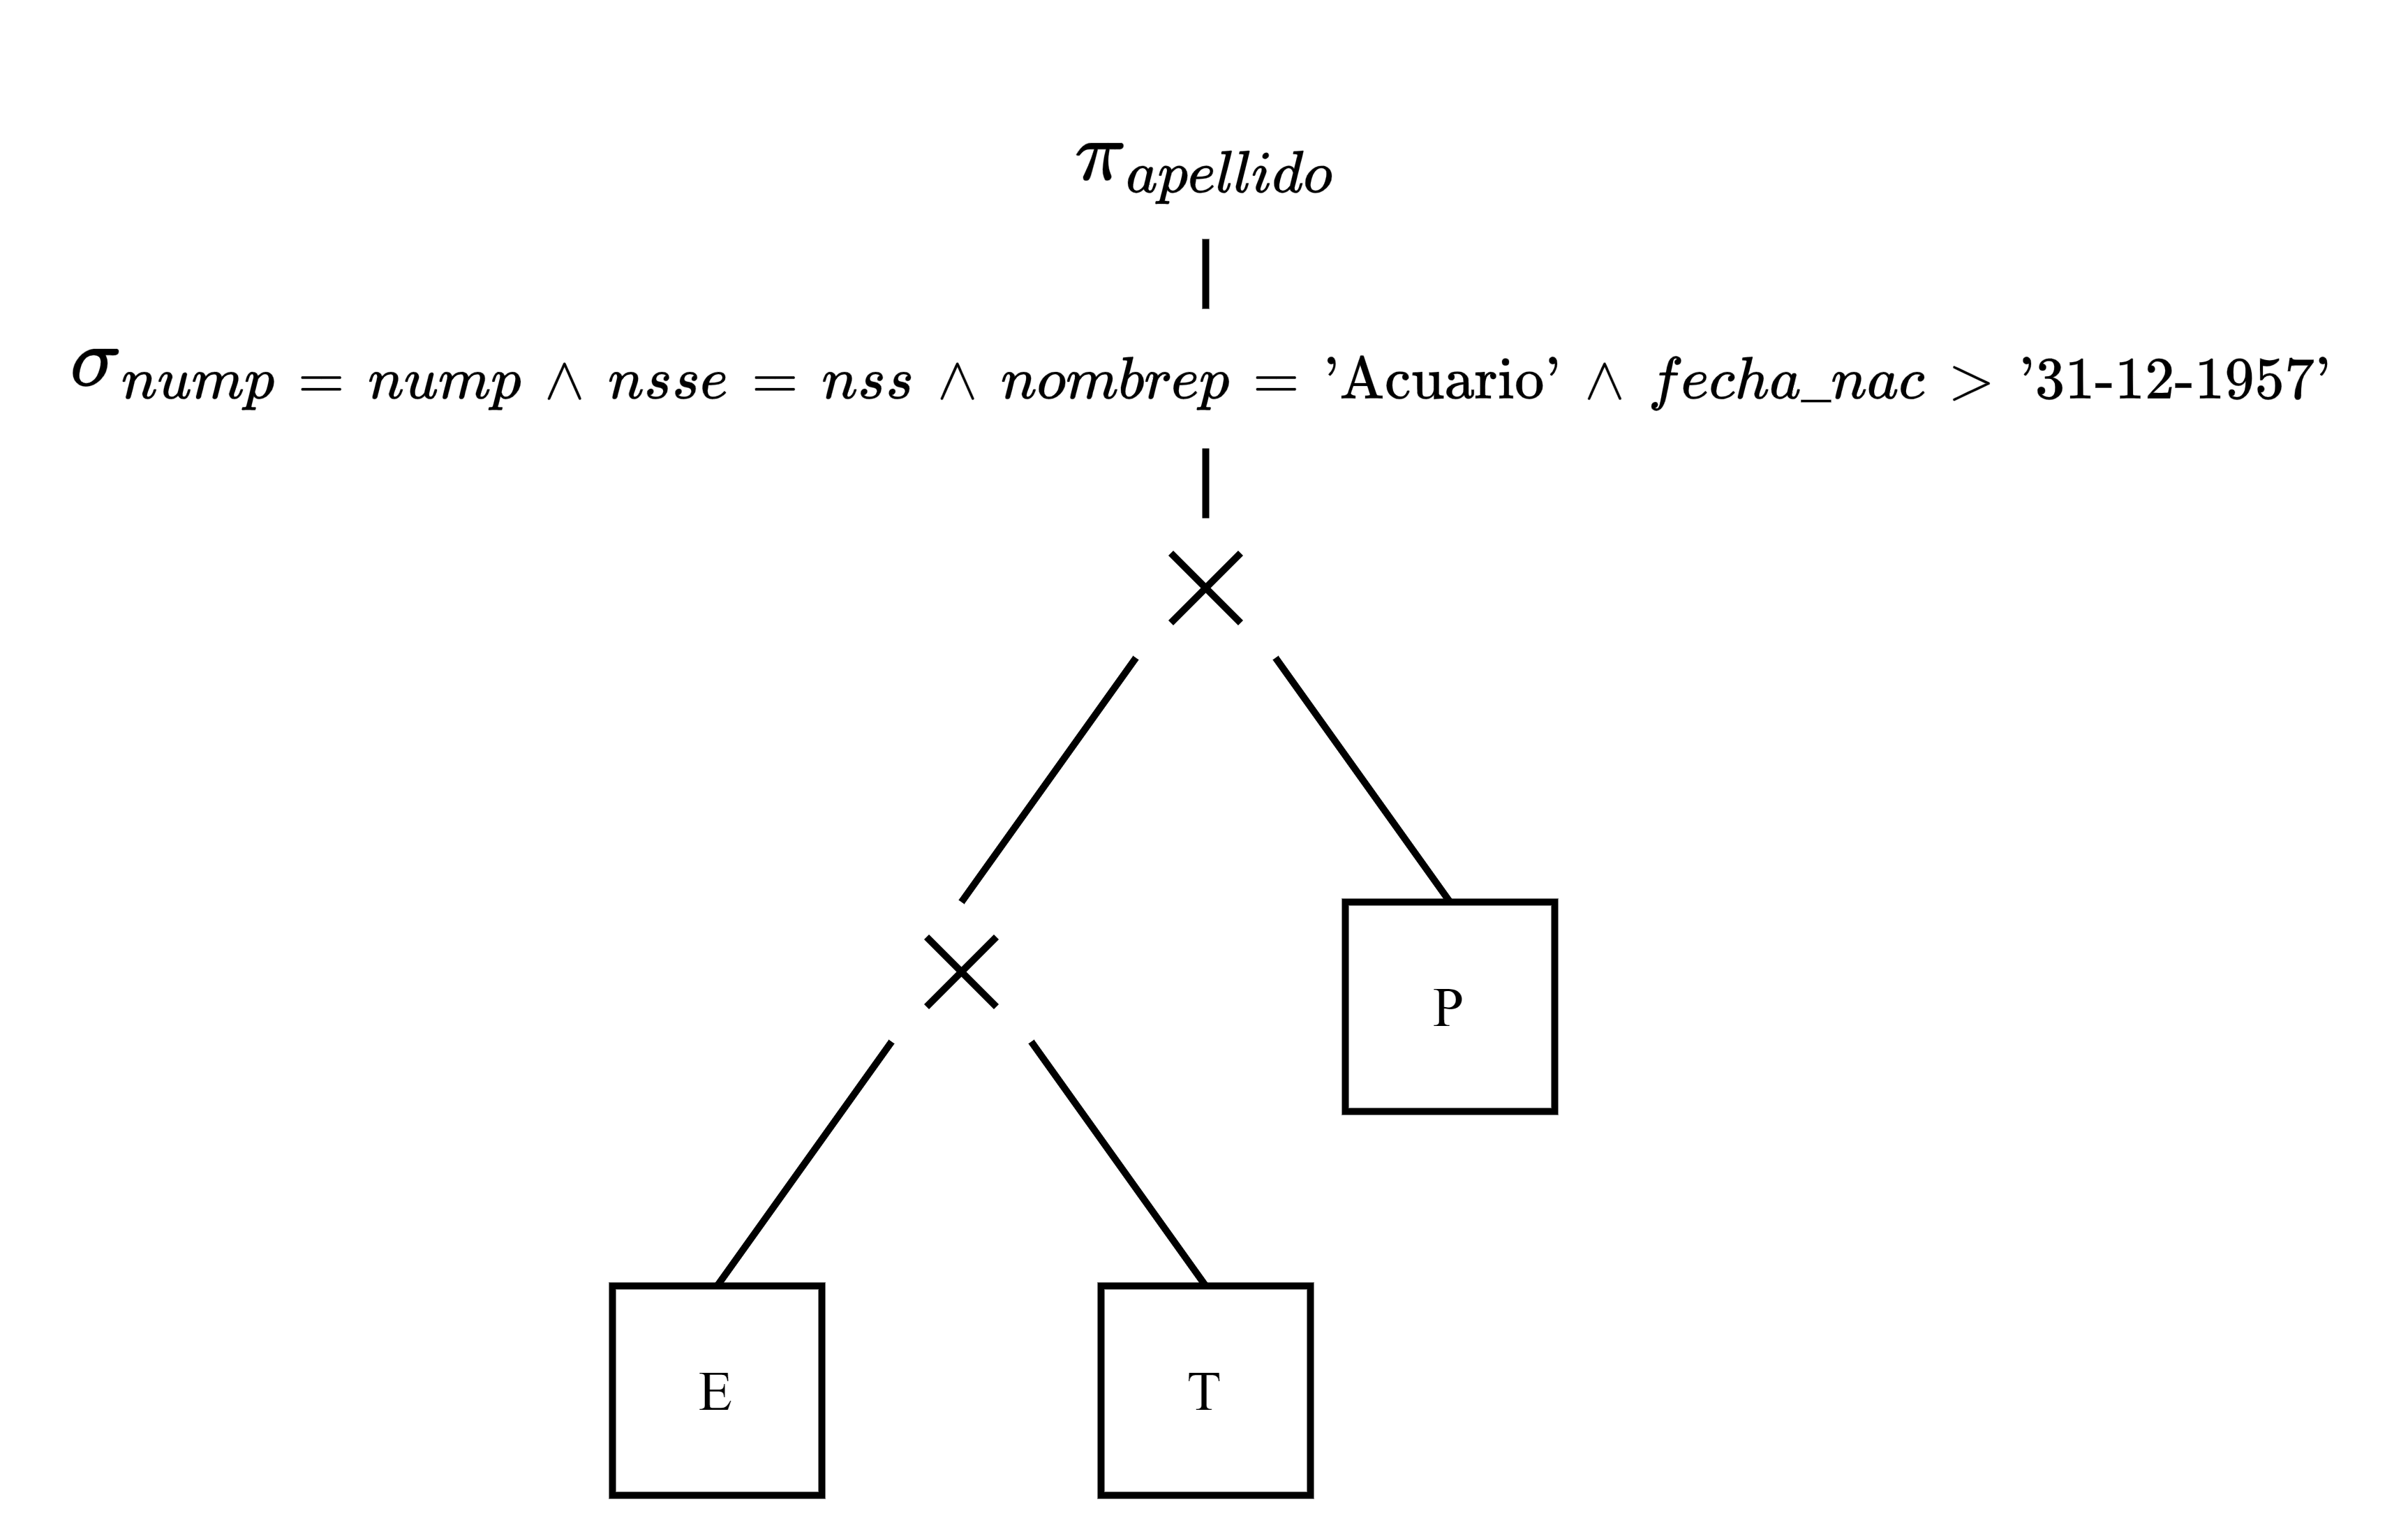
\includegraphics[width=0.8\textwidth]{img/E5-Canonico.png}
    \end{figure}

    \item Optimizaci\'on.
    \begin{enumerate}
        \item Separar las selecciones.
        \begin{figure}[H]
            \centering
            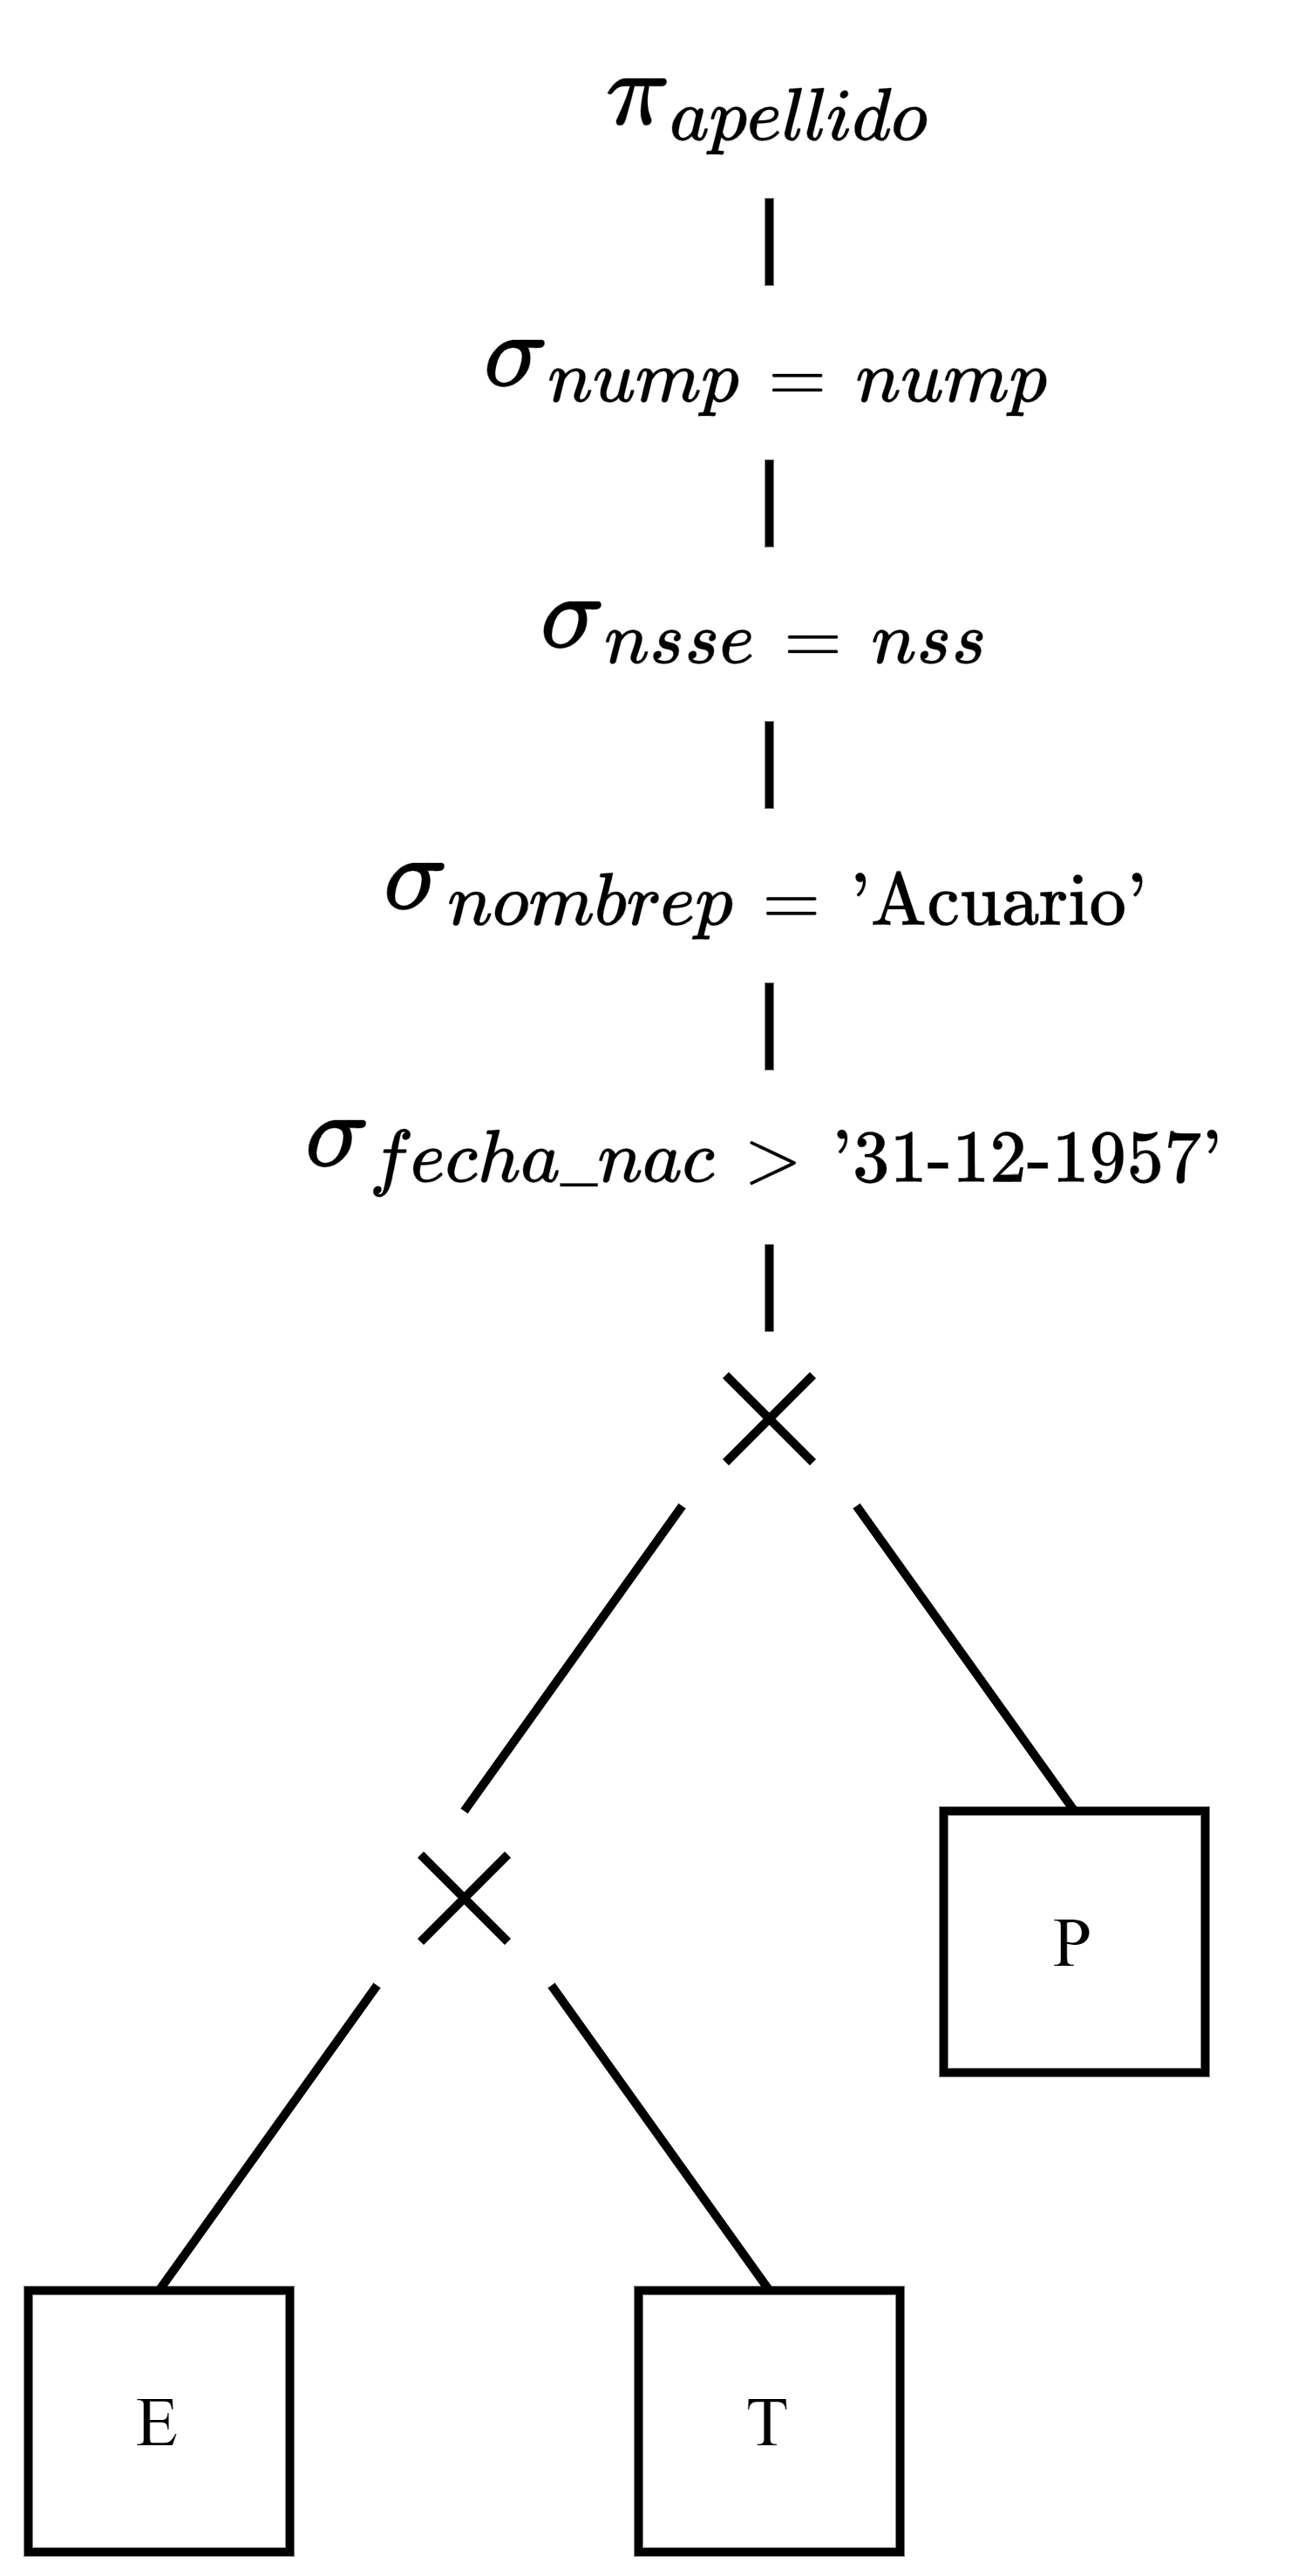
\includegraphics[width=0.4\textwidth]{img/E5-Paso-1.png}
        \end{figure}

        \newpage
        \item Permutar tablas si es necesario.
        \begin{figure}[H]
            \centering
            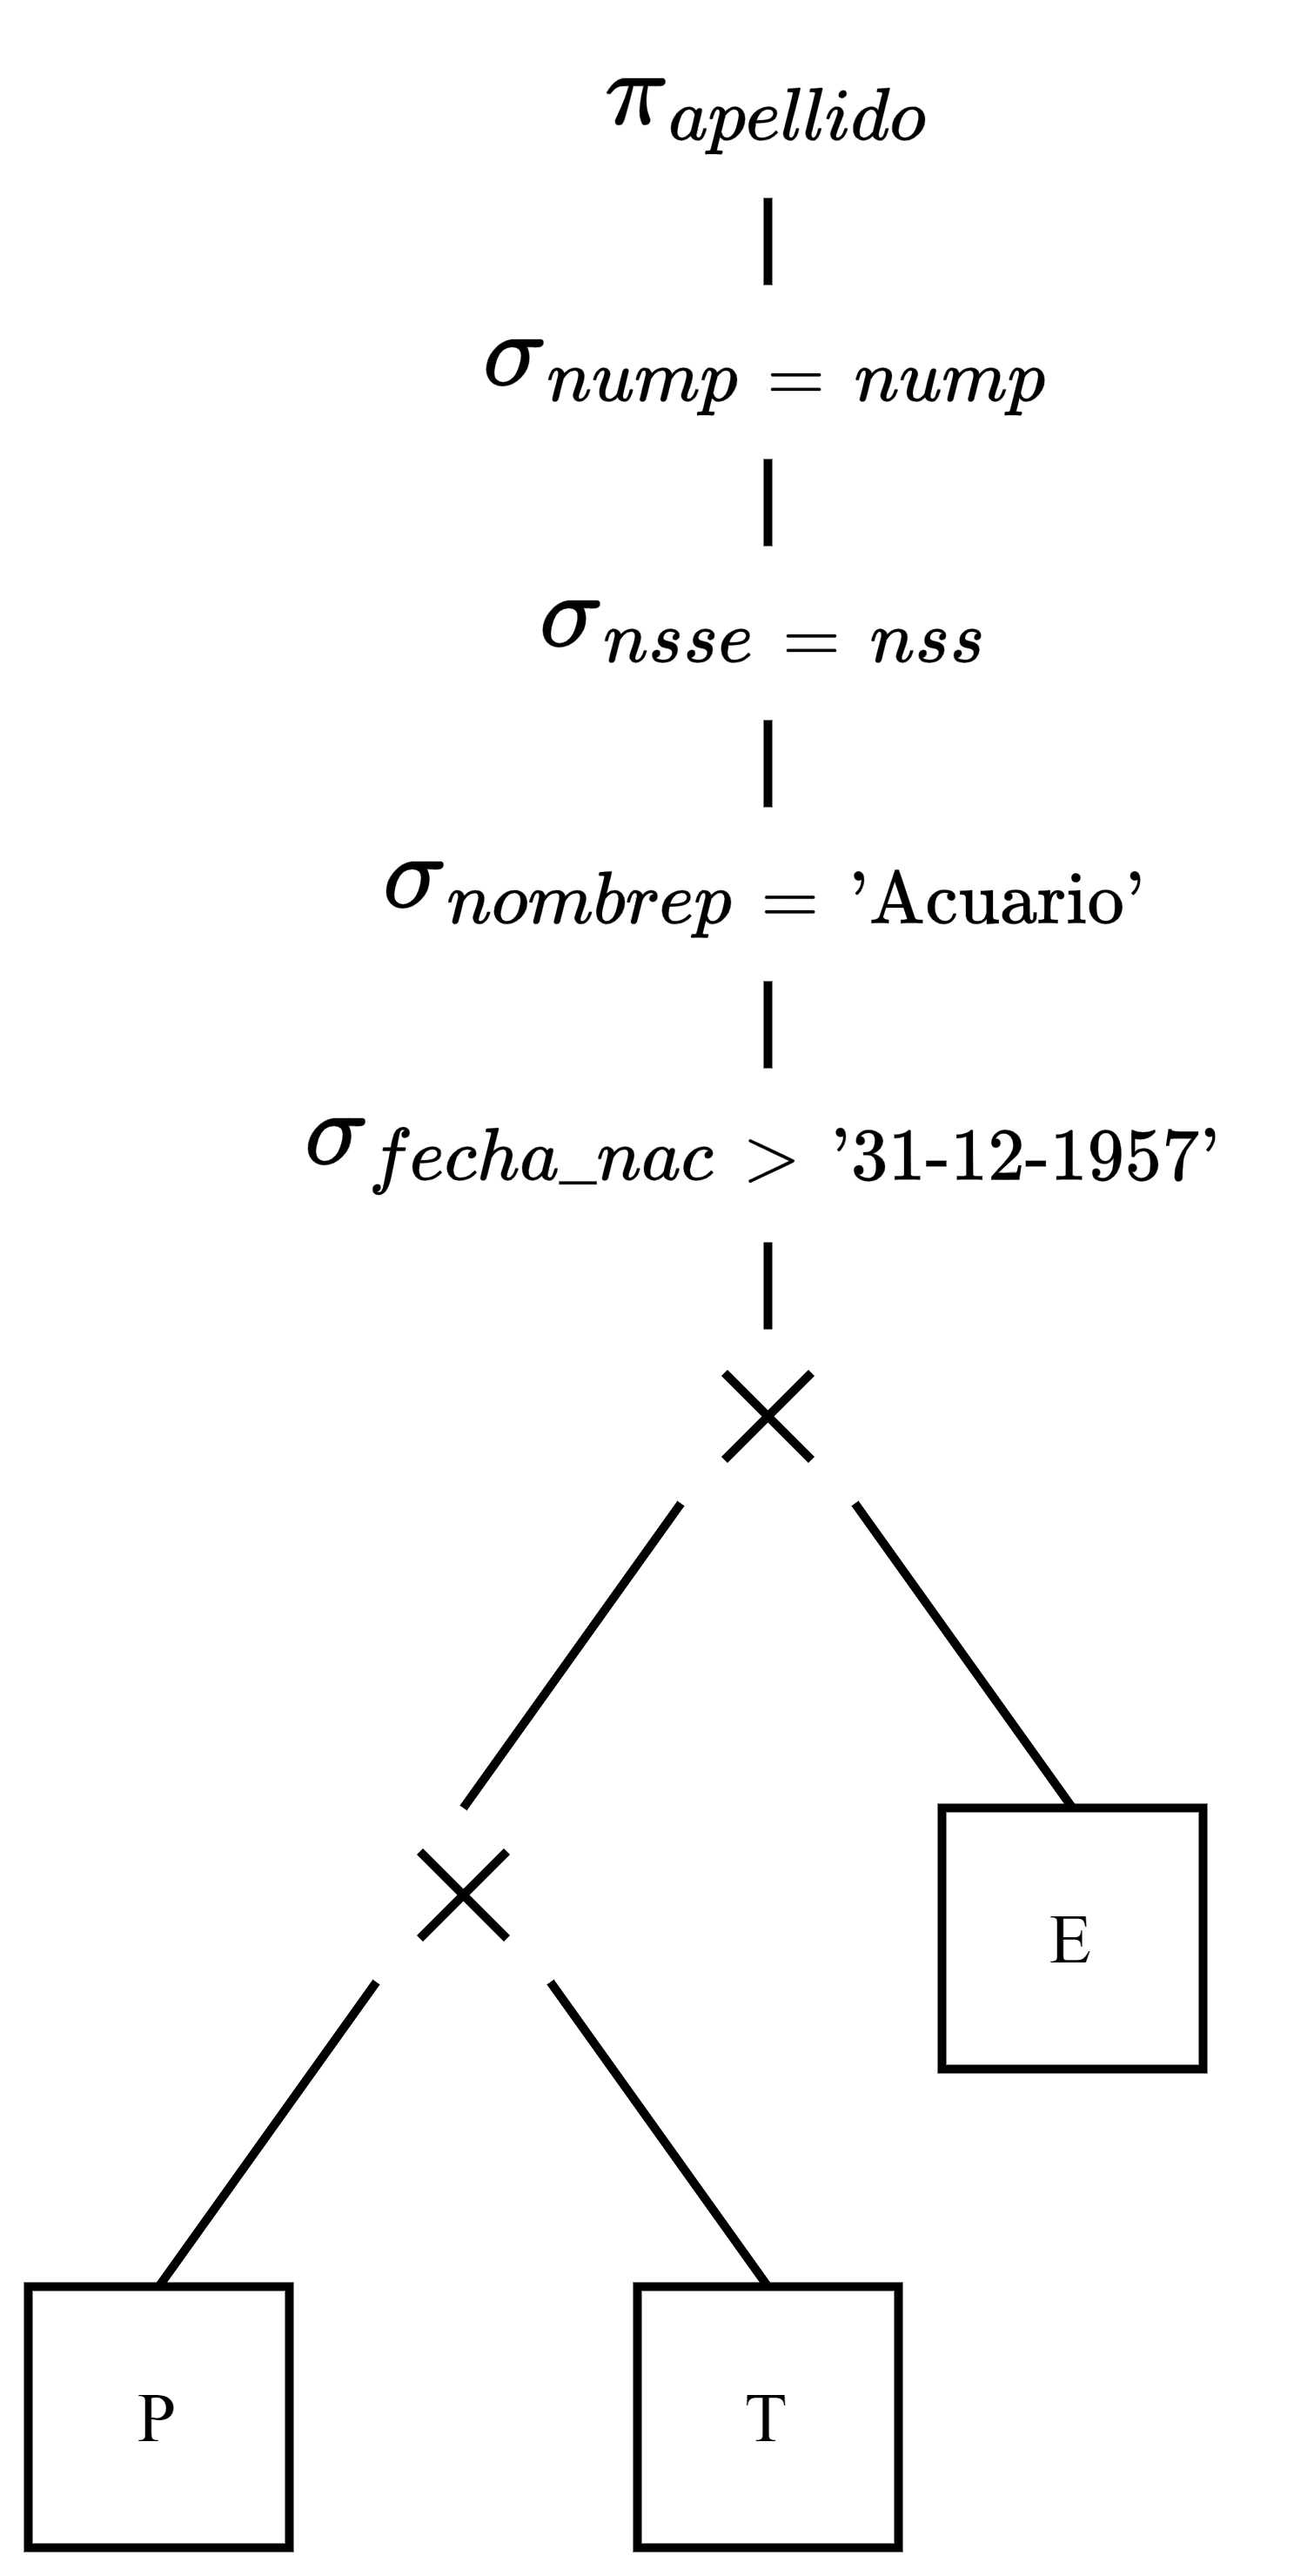
\includegraphics[width=0.35\textwidth]{img/E5-Paso-2.png}
        \end{figure}

        \item Bajar las seleciones que son $\times$ para $\Join$.
        \begin{figure}[H]
            \centering
            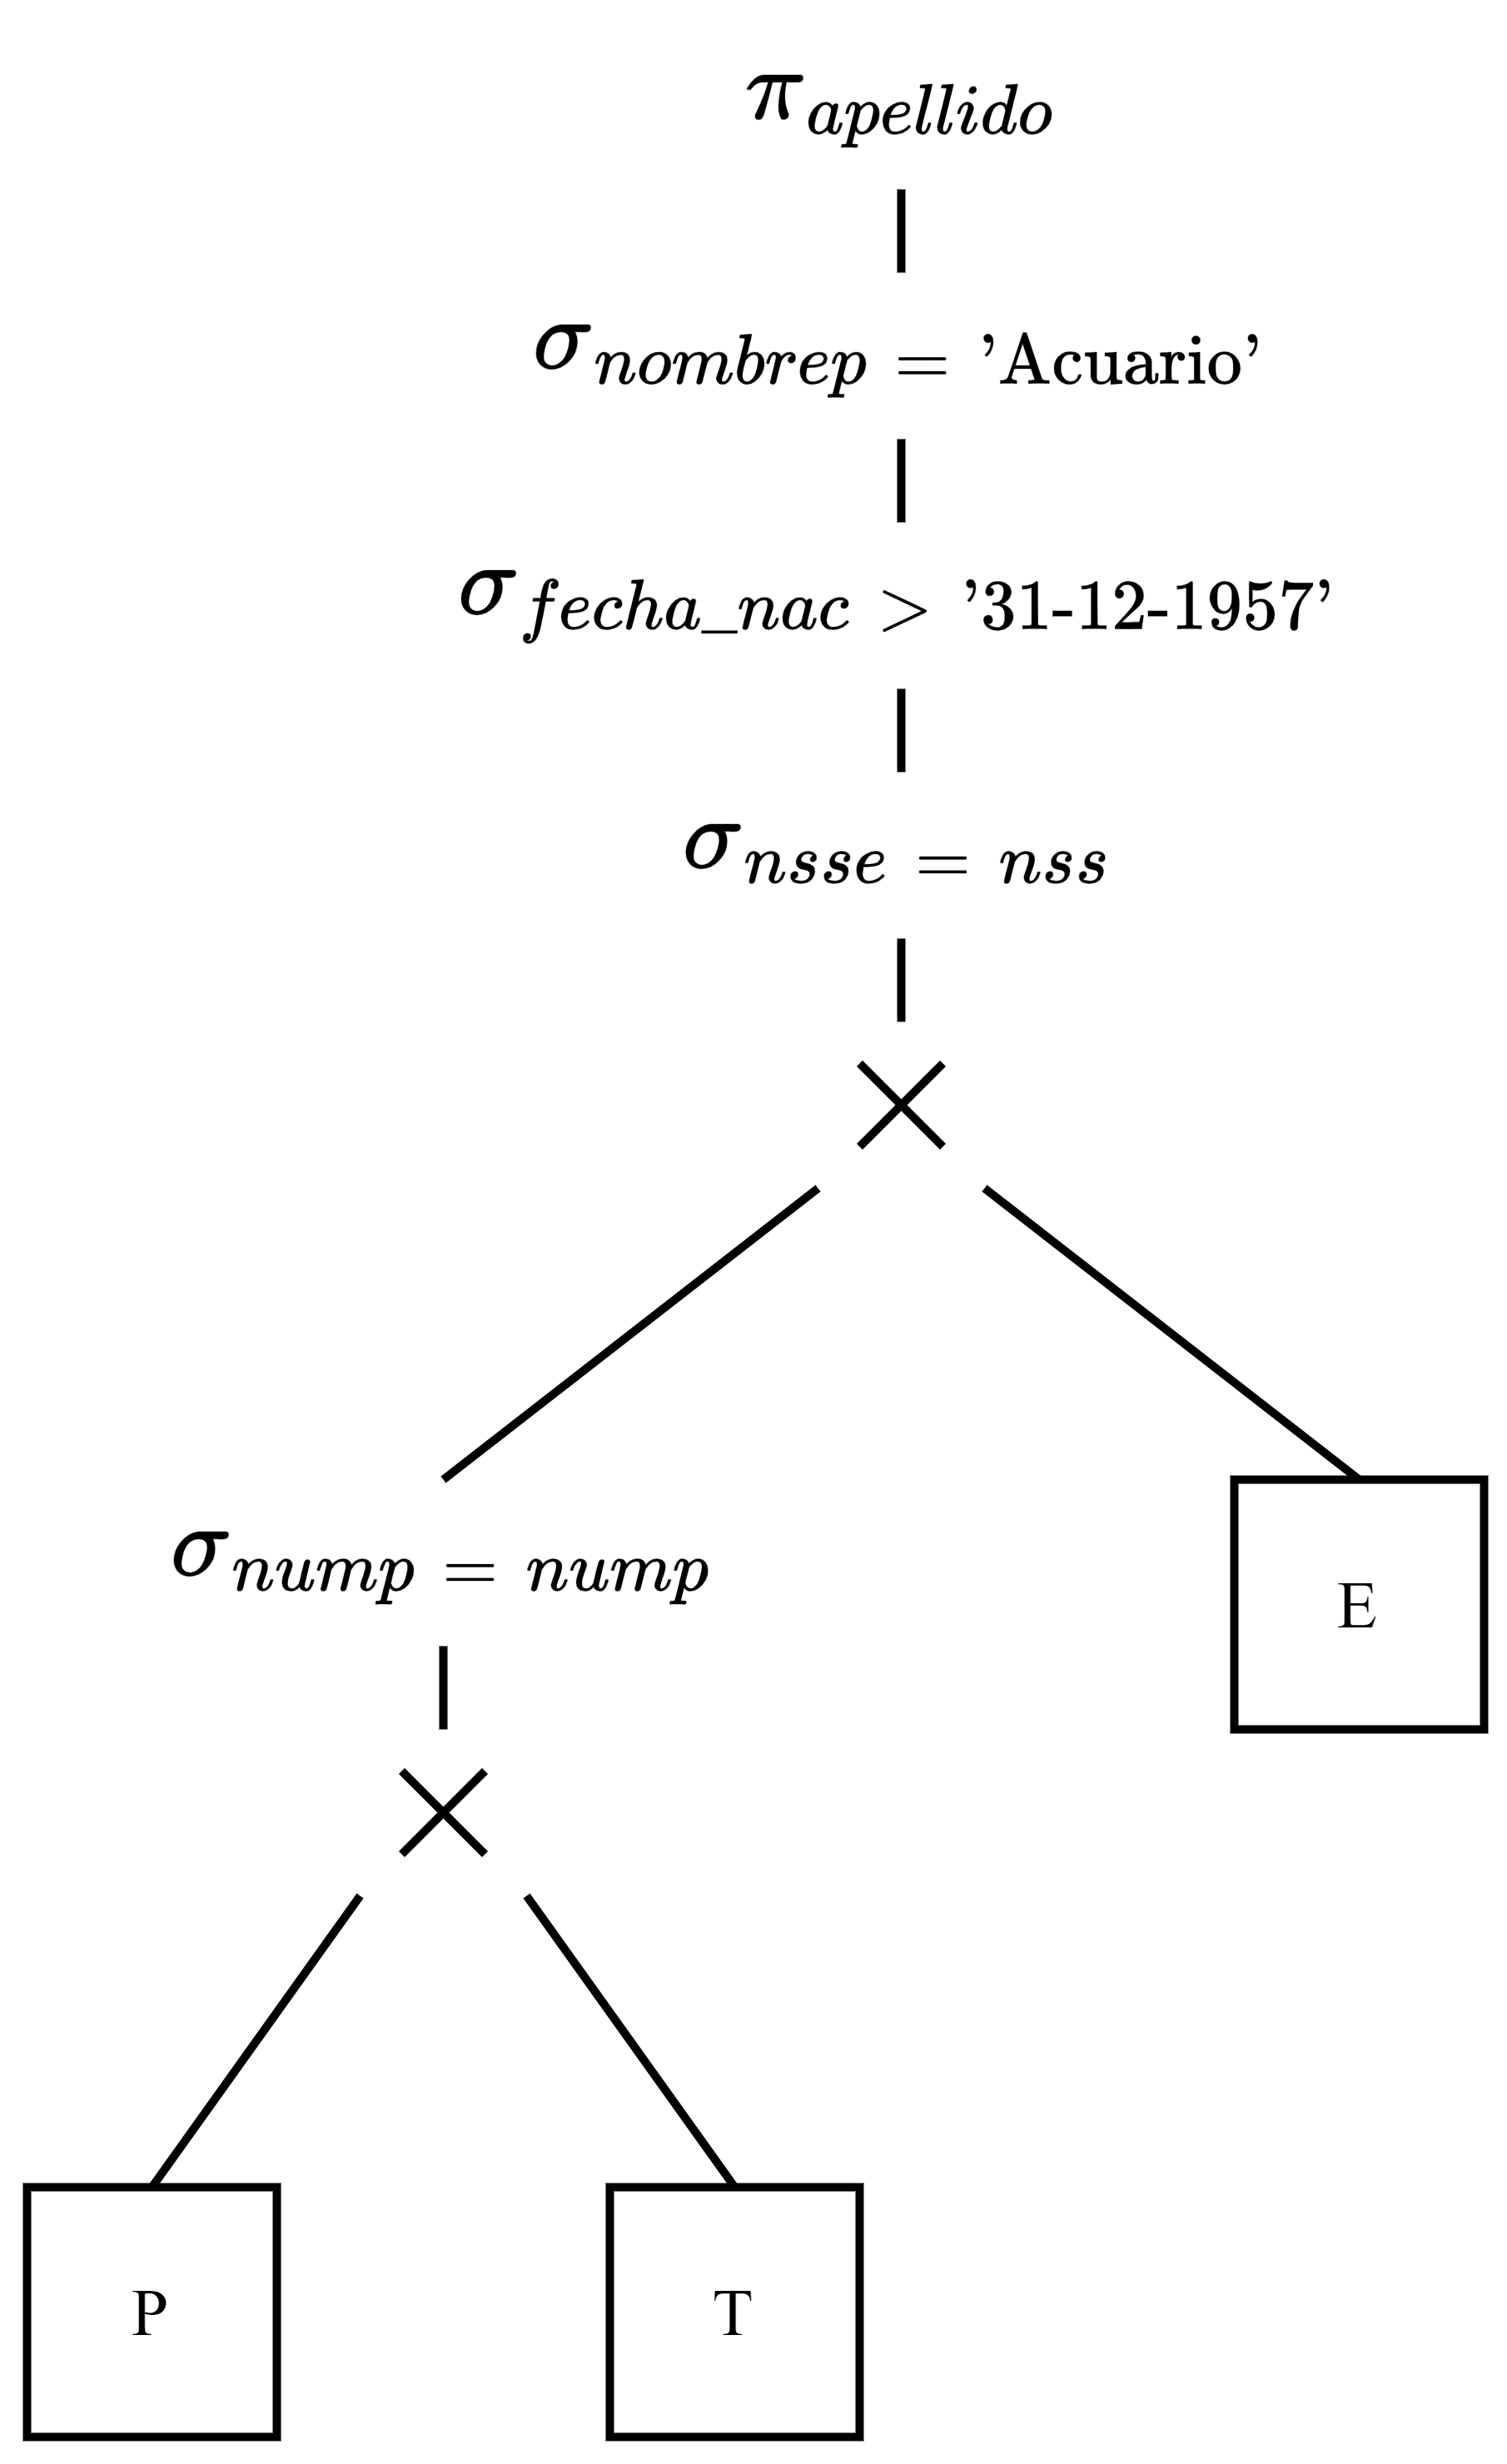
\includegraphics[width=0.4\textwidth]{img/E5-Paso-3.png}
        \end{figure}

        \item Cambio $\times$ por $\Join$.
        \begin{figure}[H]
            \centering
            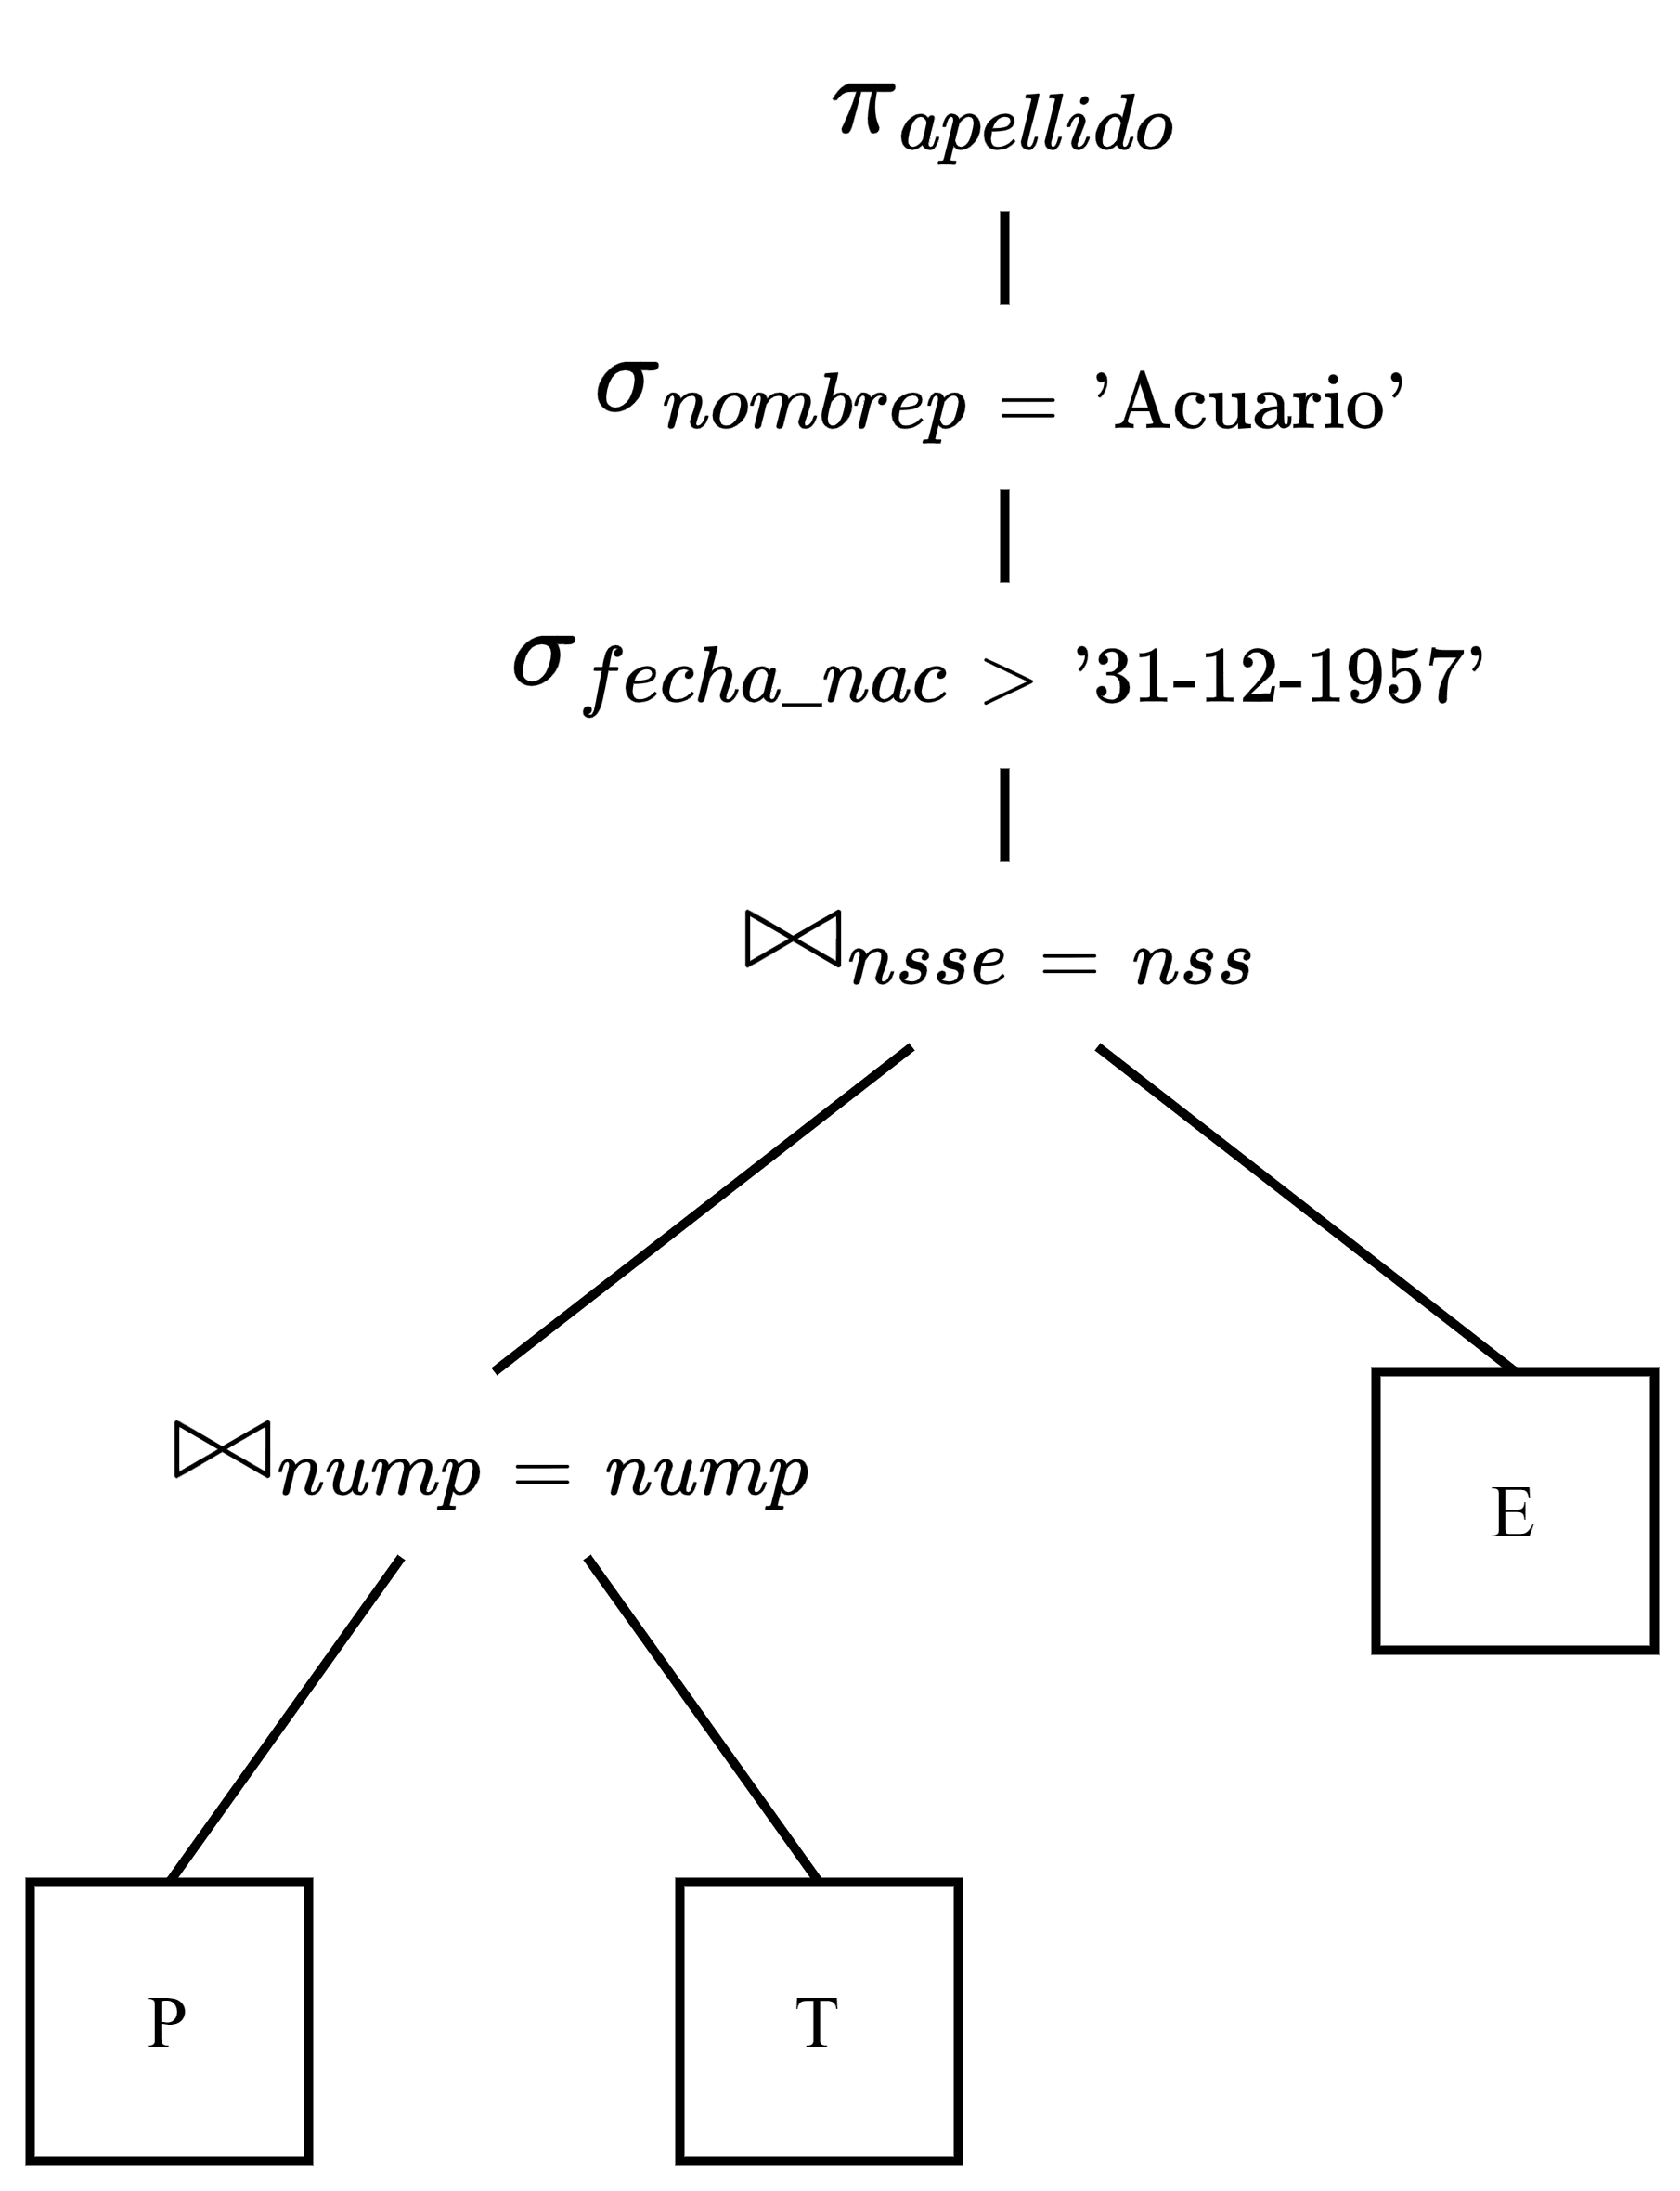
\includegraphics[width=0.5\textwidth]{img/E5-Paso-4.png}
        \end{figure}

        \item Bajar el resto de seleciones a tablas.
        \begin{figure}[H]
            \centering
            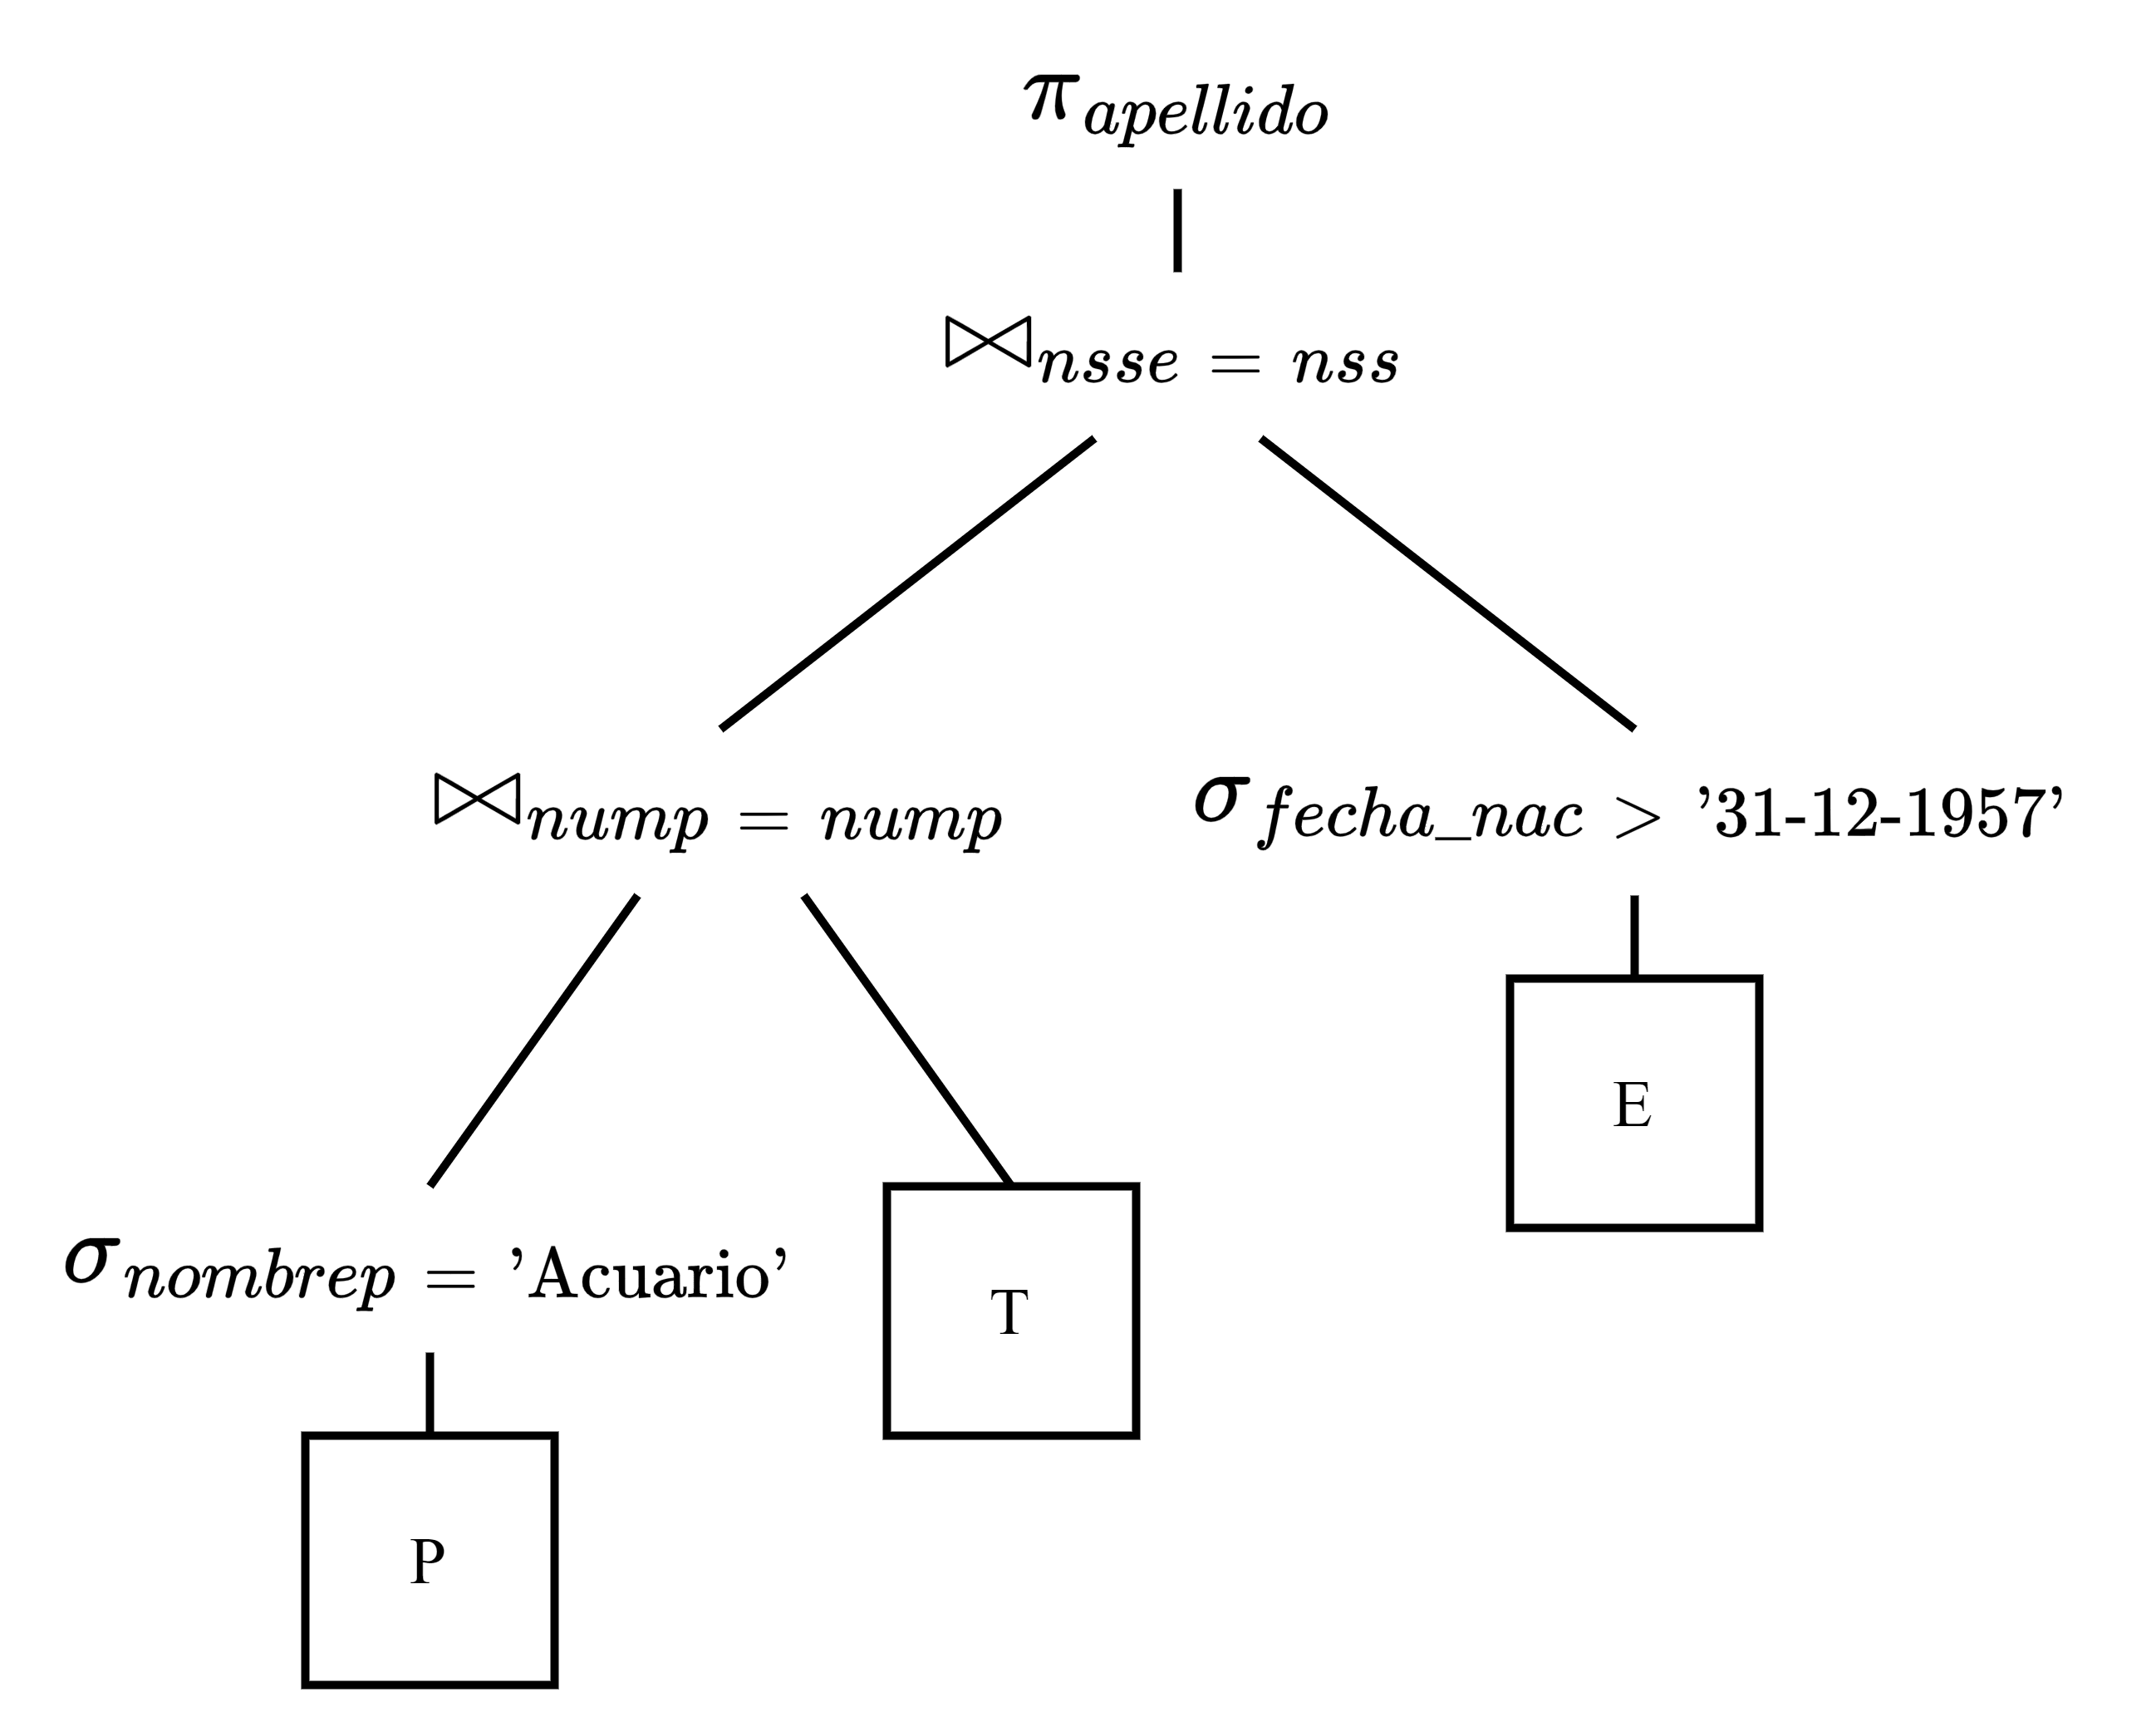
\includegraphics[width=0.6\textwidth]{img/E5-Paso-5.png}
        \end{figure}

        \newpage
        \item Proyectar los atributos necesarios.
        \begin{figure}[H]
            \centering
            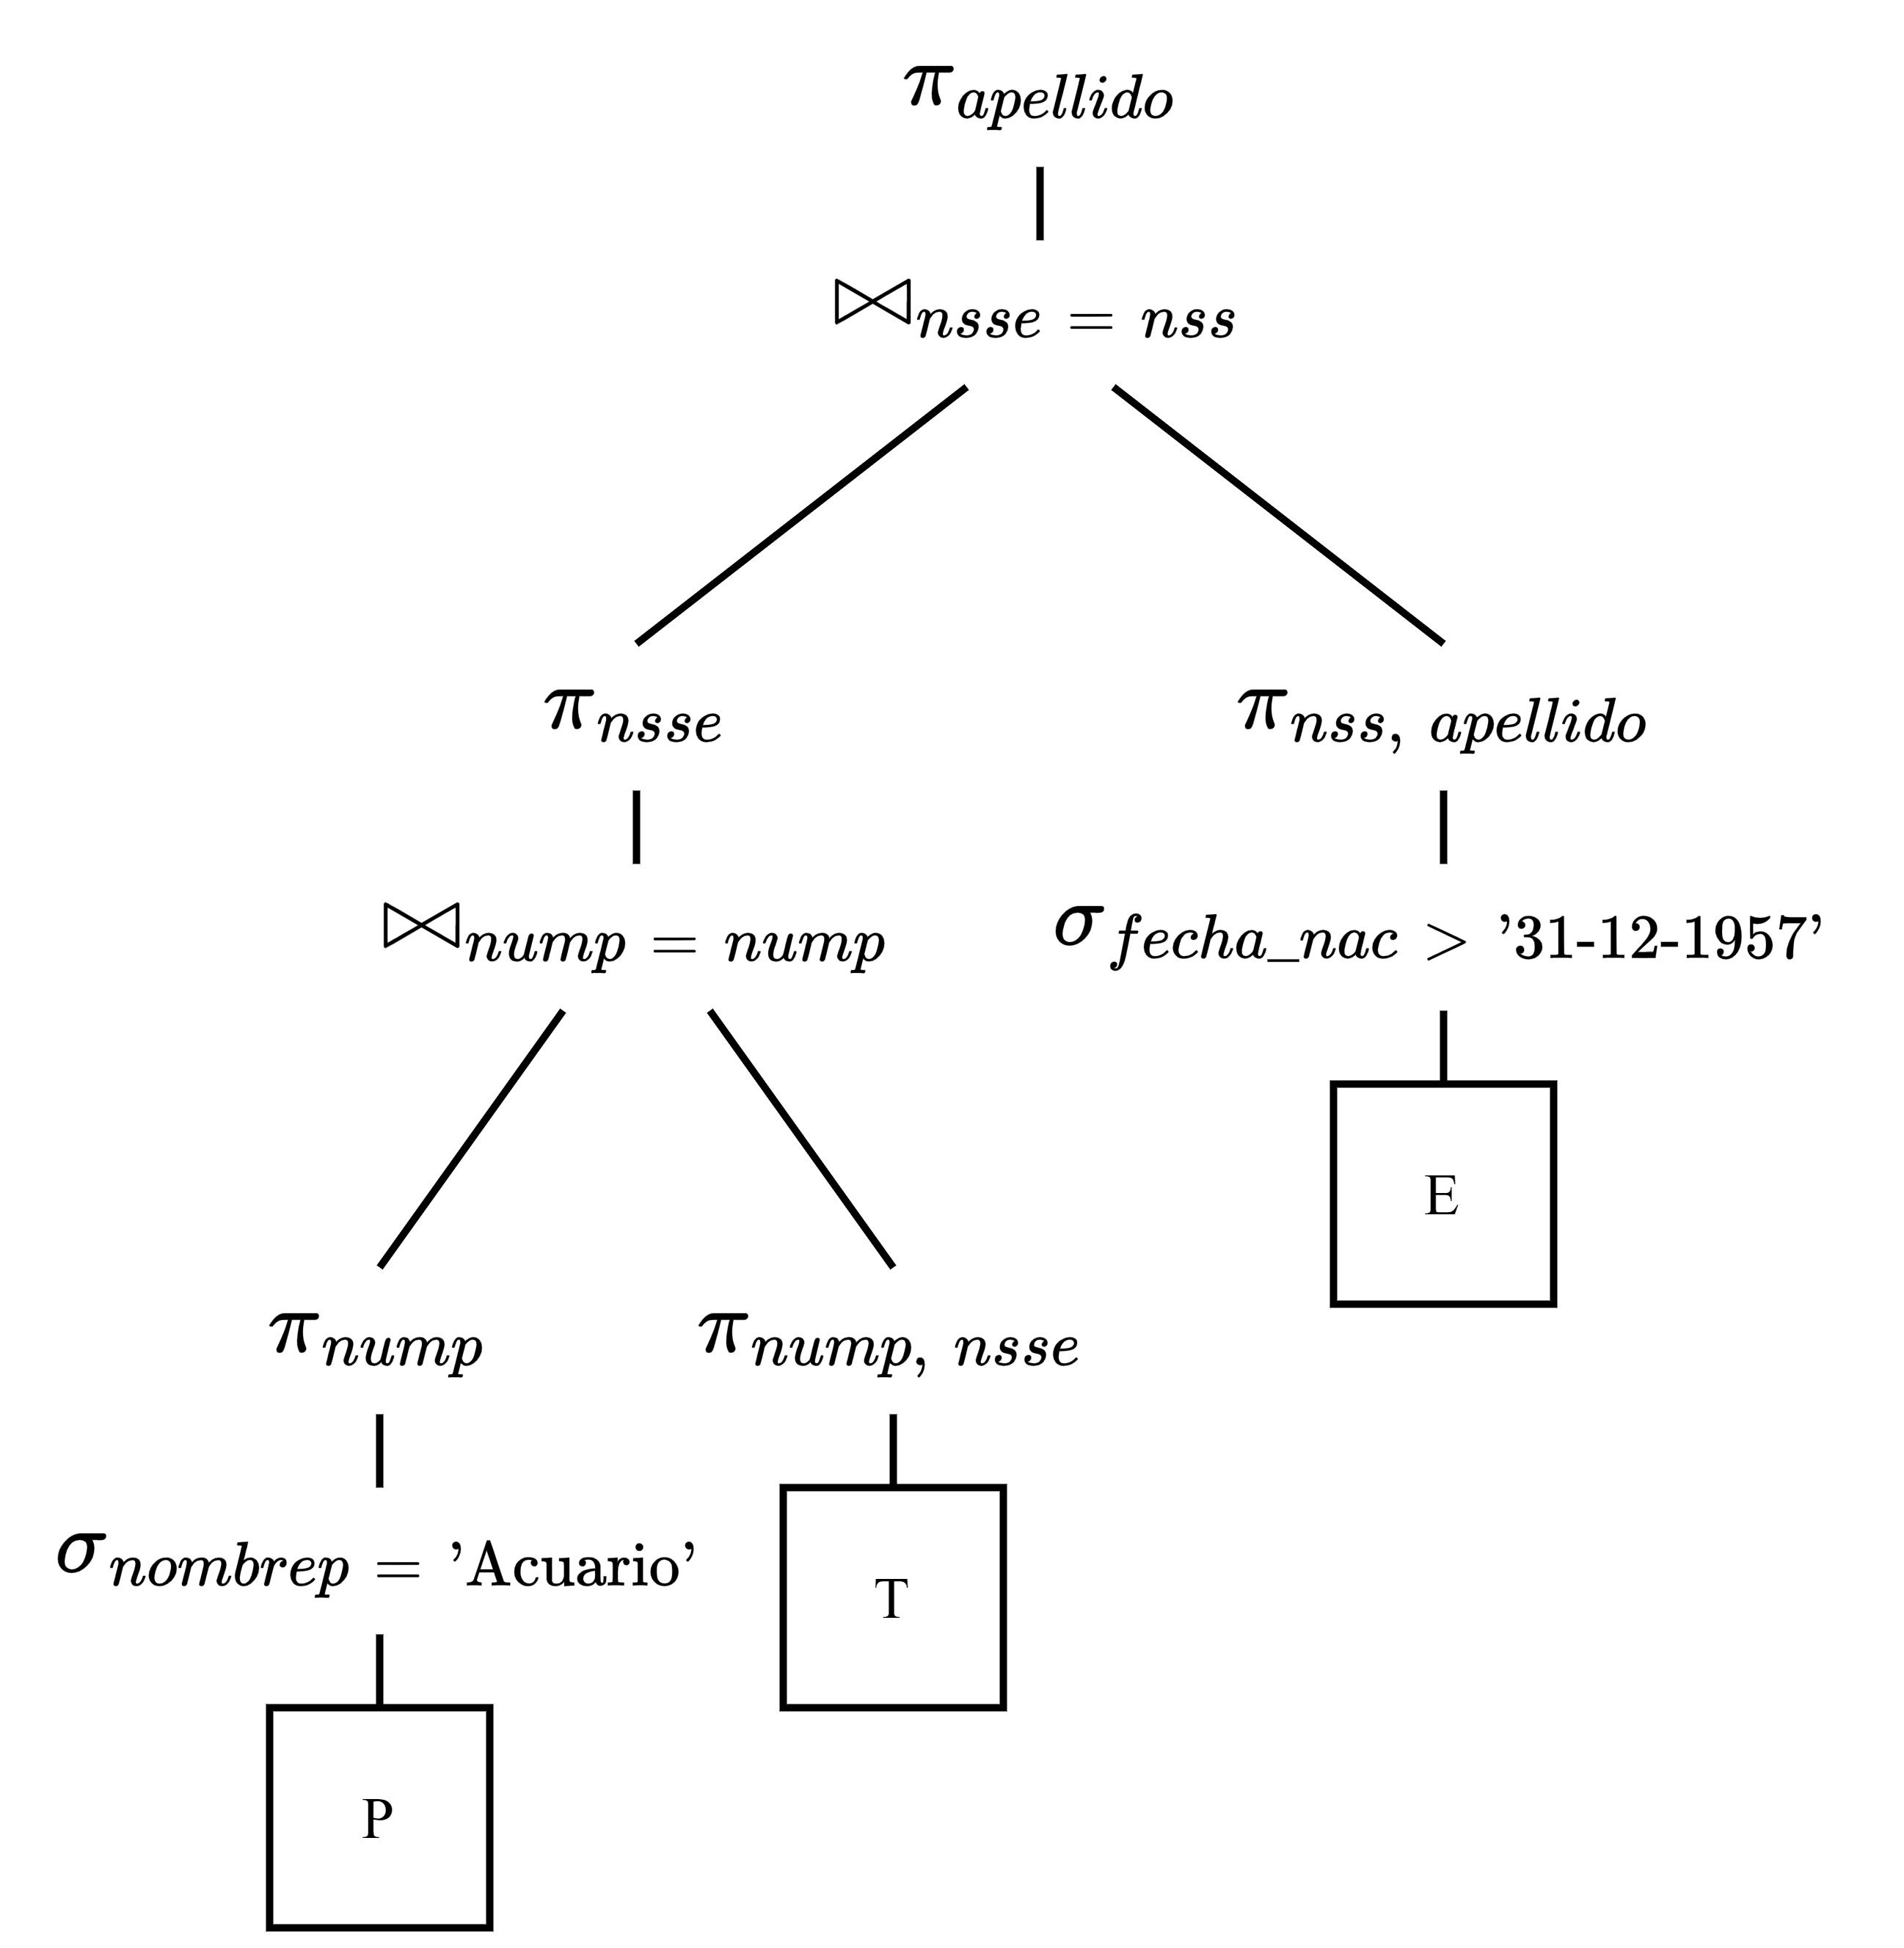
\includegraphics[width=0.7\textwidth]{img/E5-Paso-6.png}
        \end{figure}
    \end{enumerate}
\end{itemize}

\textbf{Enunciado 2:}\newline
Pegar desde un ppt (preguntarle a la profesora cual es exactamente).
\begin{itemize}
    \item SQL.
    \begin{verbatim}
SELECT Nmicro NM,
       Nempresa NE,
       Nomempresa E,
       fechacreacion fc,
       direccion dir,
       destino dest,
       fecha_viaje fv
FROM Viaje V,
     Empresa EP,
     Micro M
WHERE M.NM = V.NM
AND M.NE = EP.NE
AND EP.fc >= '01-01-2000'
AND V.fv >= '01-01-2007'
AND V.fv < '01-02-2007'
ADN M.marca = 'M.Benz';
    \end{verbatim}

    \item Algebra Relacional.
    \begin{align*}
        \scalebox{1.5}{$\pi$}_{\text{NM, NE, E, fc, dir, dest, fv}} (
            \scalebox{1.5}{$\sigma$}_{
                \scalebox{0.8}{
                    $\begin{array}{l}
                        \text{NM} = \text{NM} \; \wedge \\
                        \text{NE} = \text{NE} \; \wedge \\
                        \text{fc} \geq \text{'01-01-2000'} \; \wedge \\
                        \text{fv} \geq \text{'01-01-2007'} \; \wedge \\
                        \text{fv} < \text{'01-02-2007'} \; \wedge  \\
                        \text{marca} = \text{'M.Benz'}
                    \end{array}$
                }
            } (
                \text{V}_{\scalebox{1.3}{$\Join$}} (
                    \text{EP}_{\scalebox{1.3}{$\Join$}} \text{M}
                )
            )
        )
    \end{align*}

    \item \'Arbol Can\'onico.
    \begin{figure}[H]
        \centering
        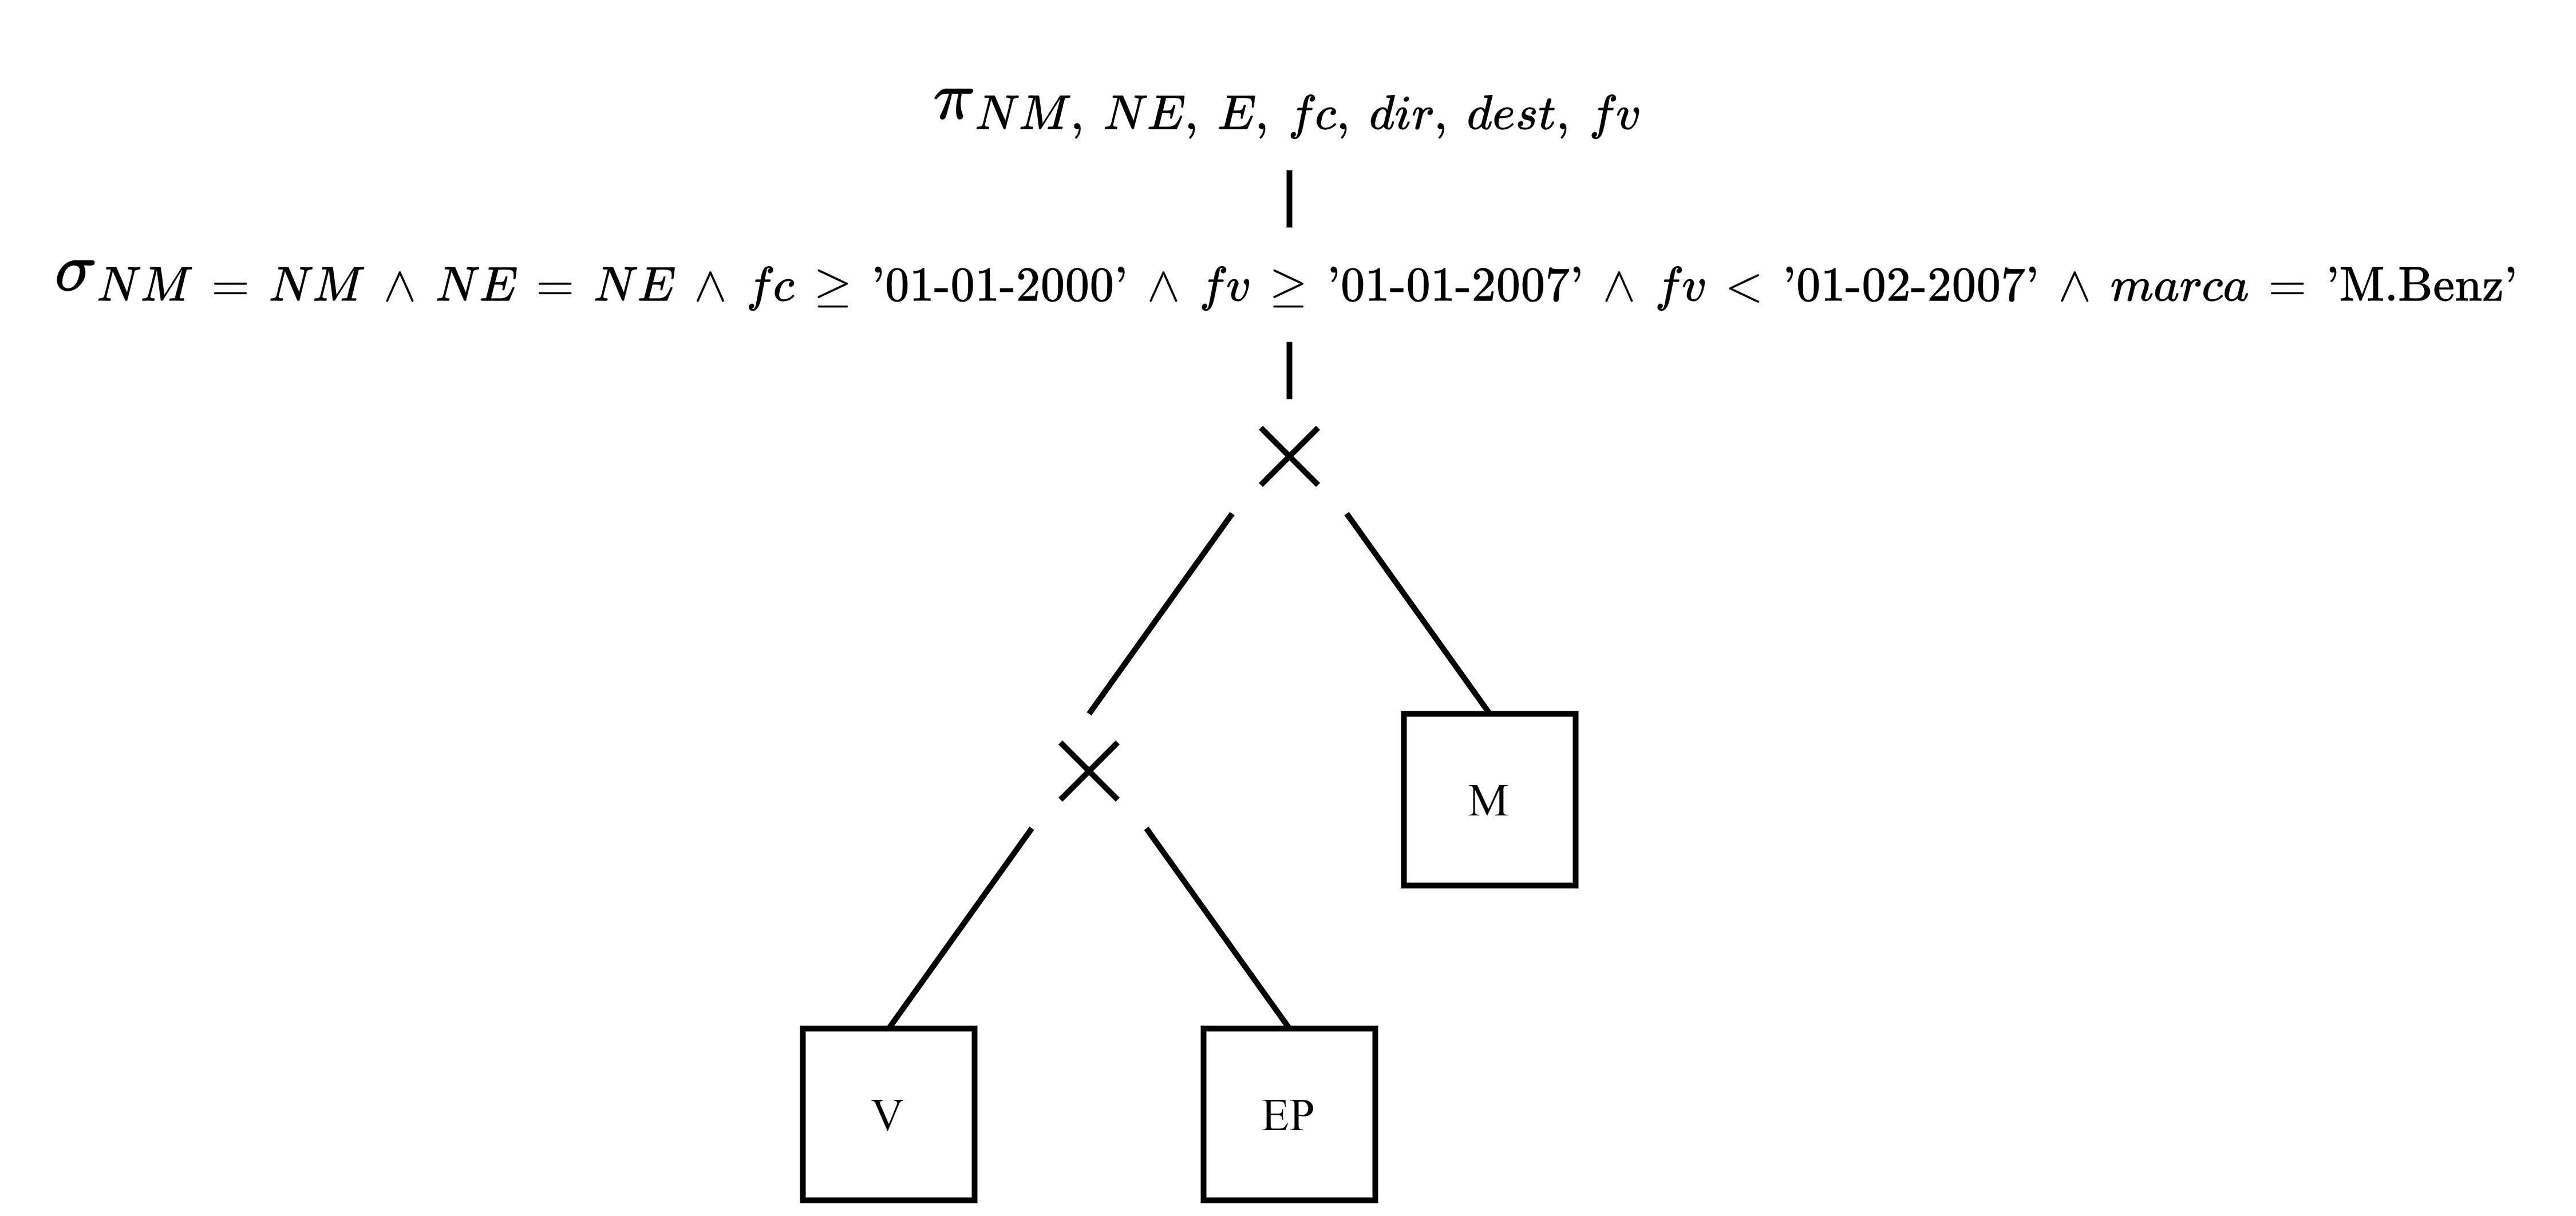
\includegraphics[width=0.8\textwidth]{img/E6-Canonico.png}
    \end{figure}

    \item Optimizaci\'on.
    \begin{enumerate}
        \item Separar las selecciones.
        \begin{figure}[H]
            \centering
            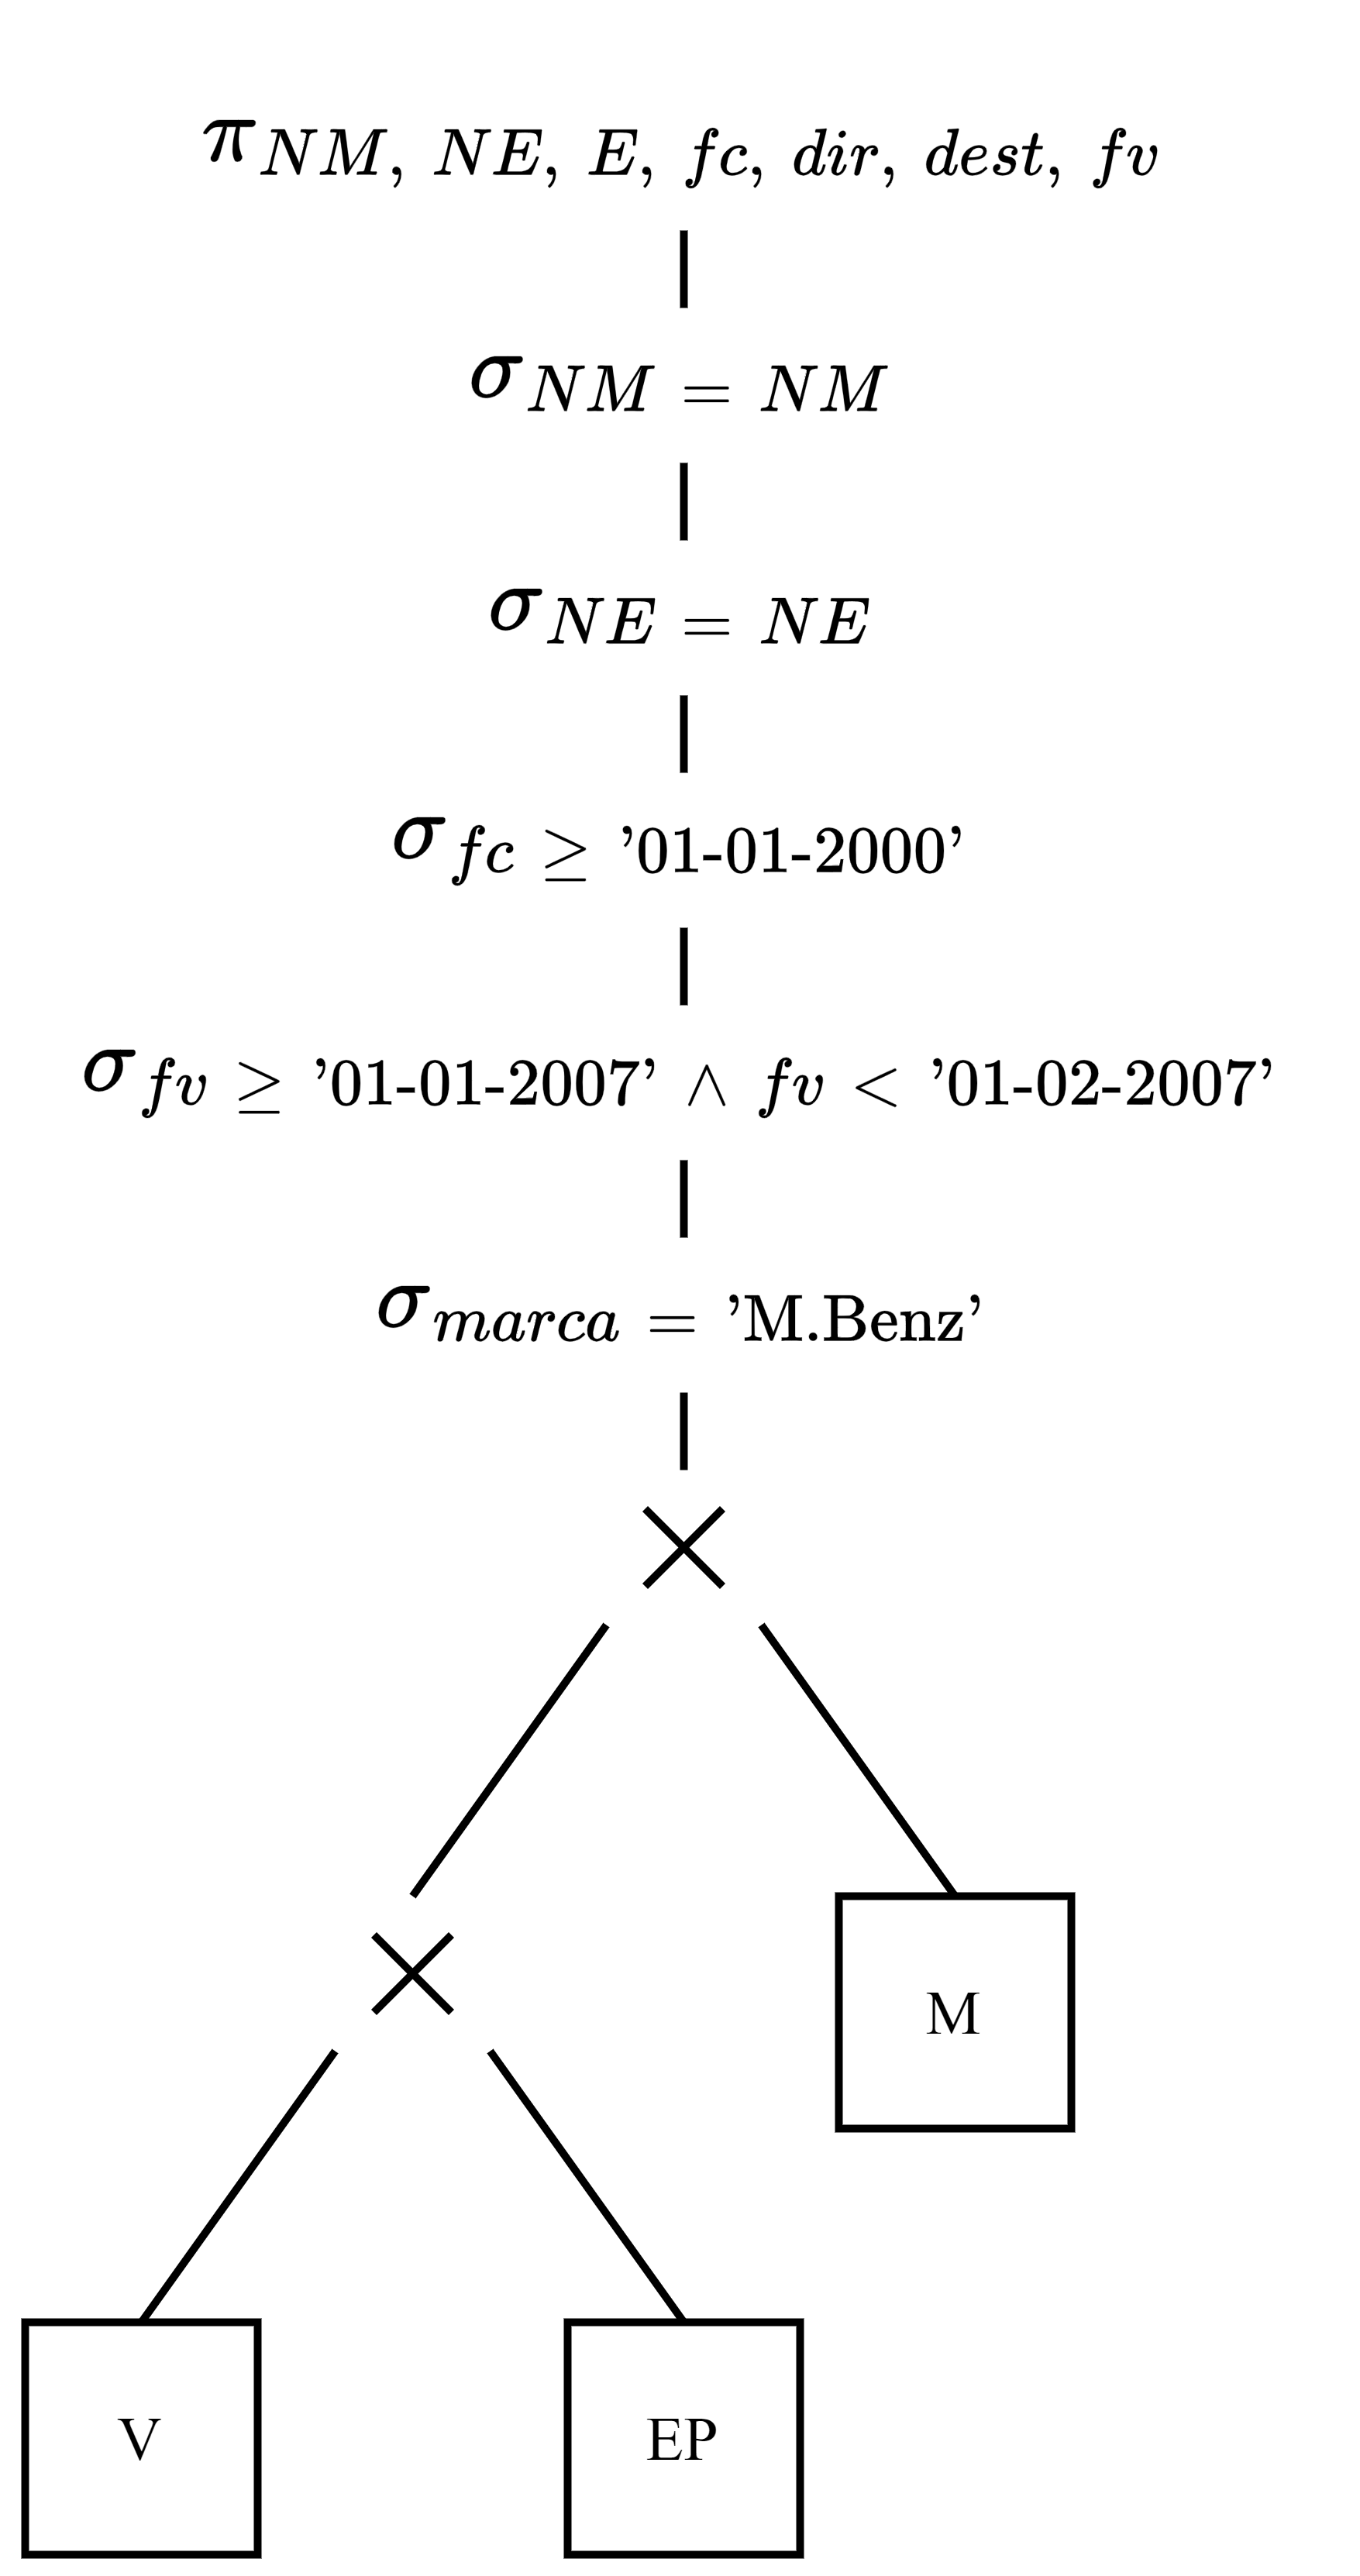
\includegraphics[width=0.3\textwidth]{img/E6-Paso-1.png}
        \end{figure}

        \newpage
        \item Permutar tablas si es necesario.
        \begin{figure}[H]
            \centering
            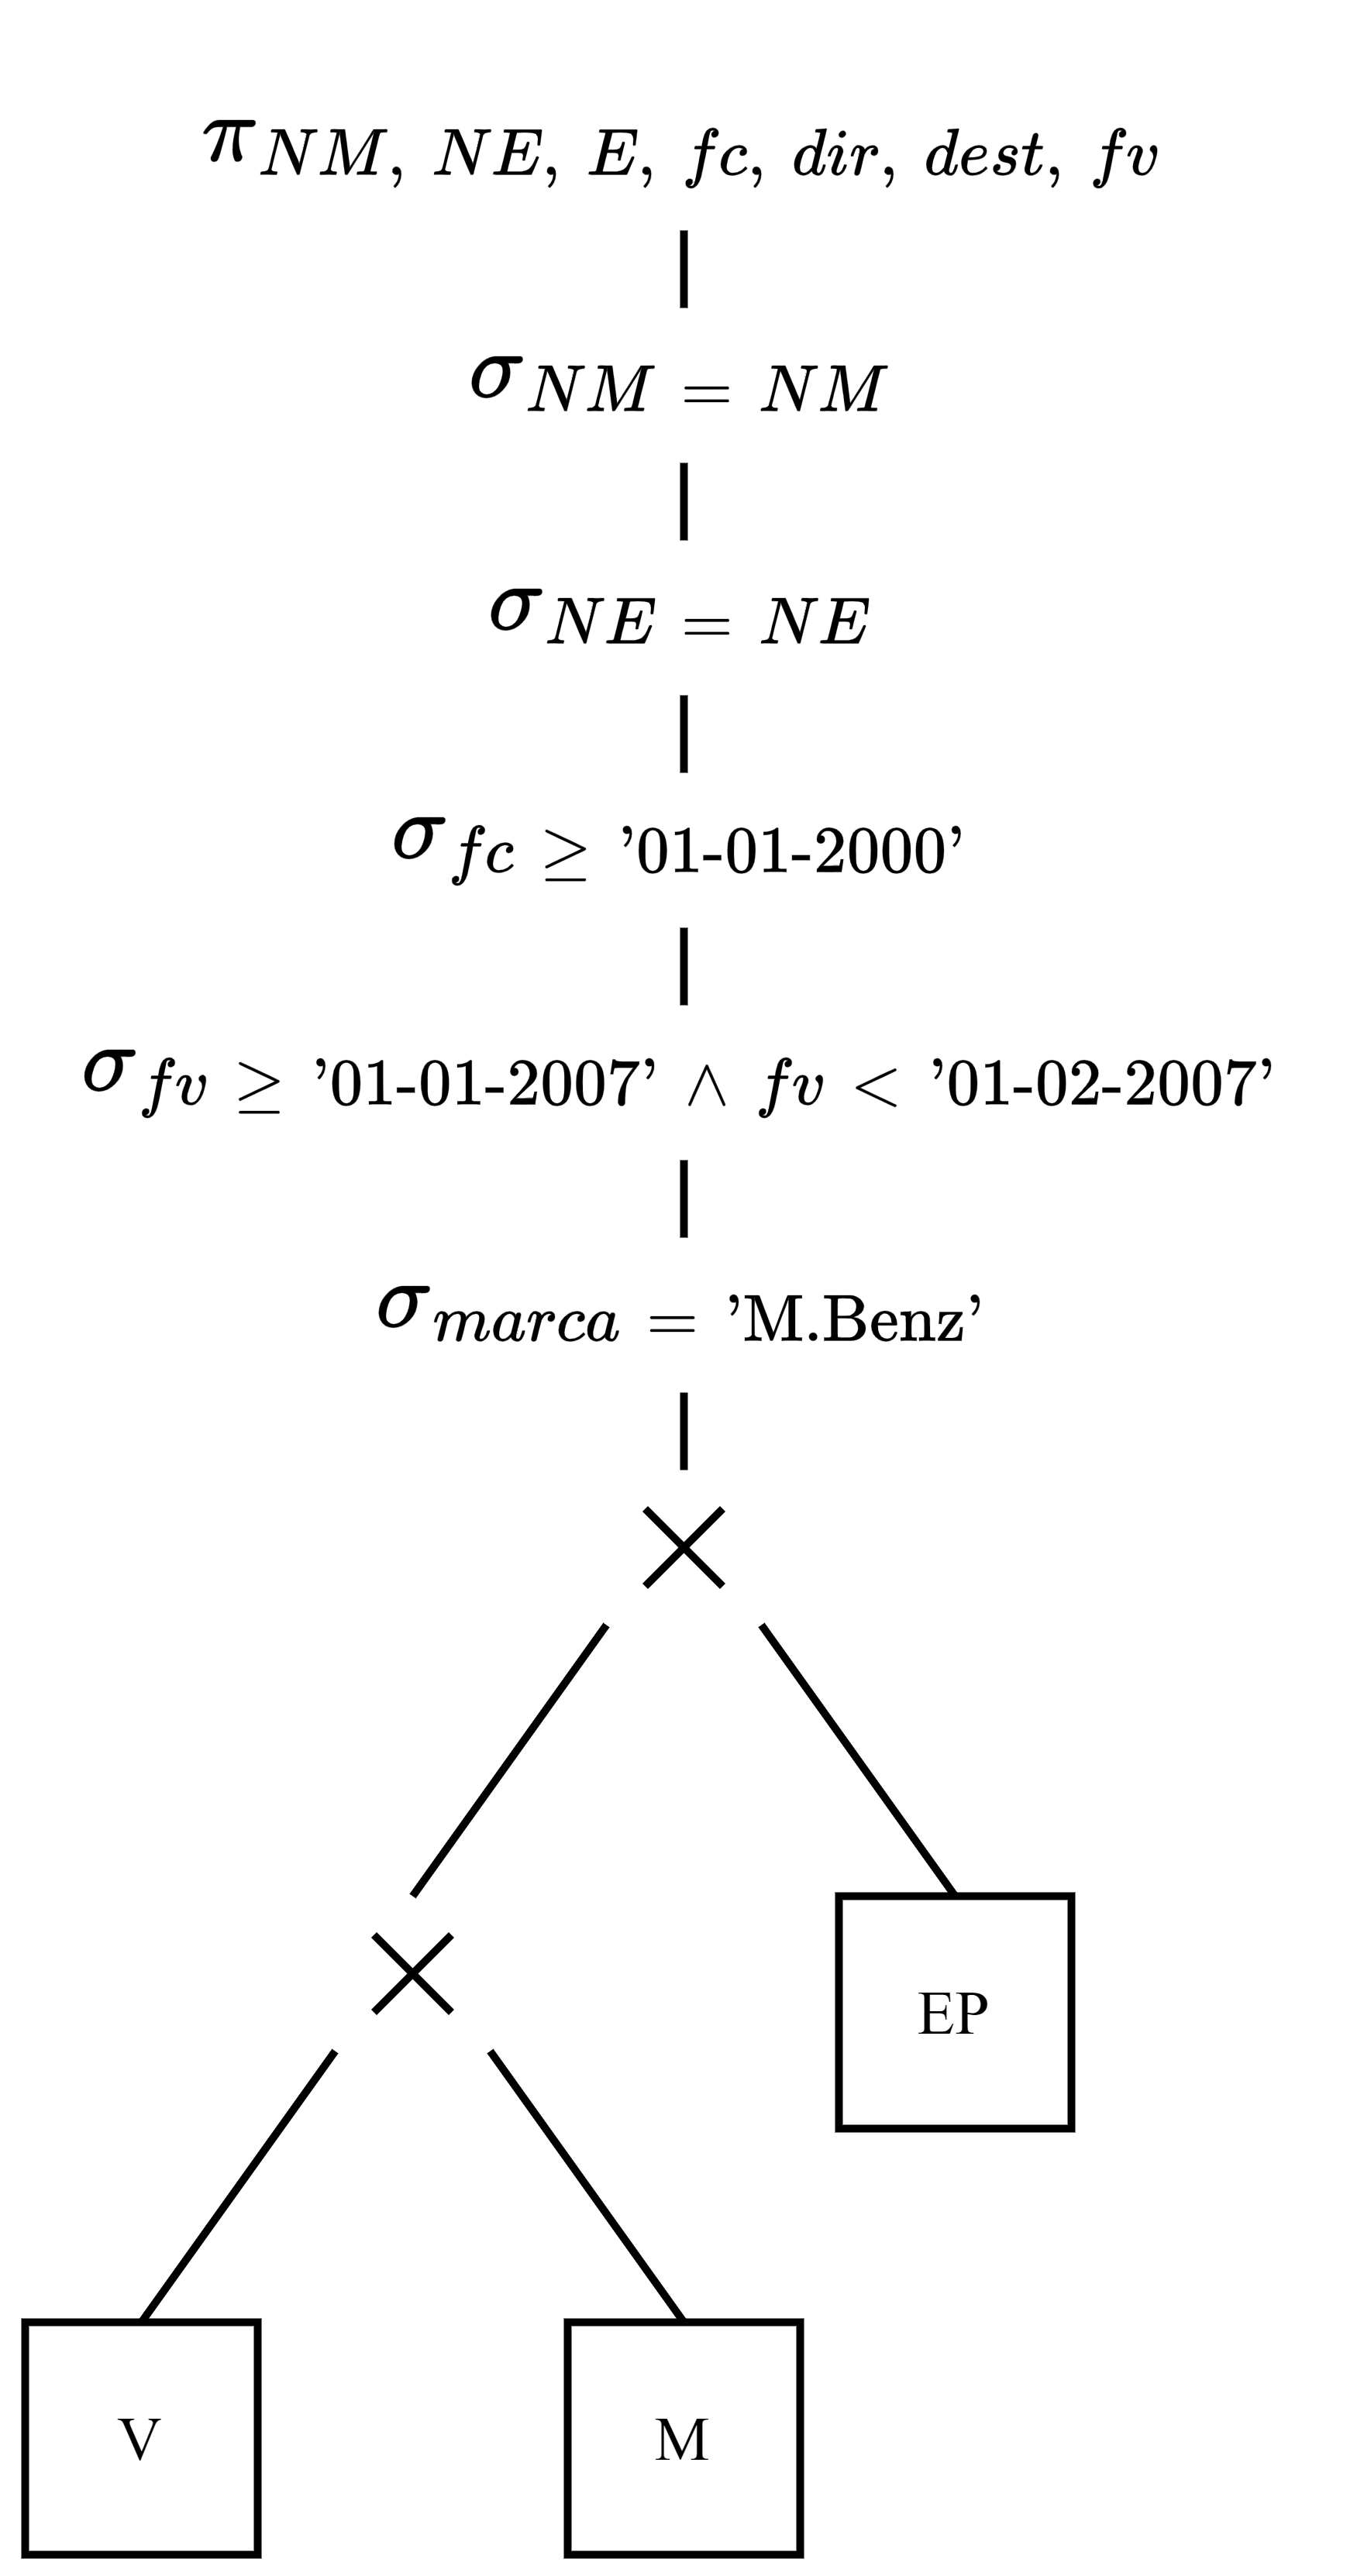
\includegraphics[width=0.35\textwidth]{img/E6-Paso-2.png}
        \end{figure}

        \item Bajar las seleciones que son $\times$ para $\Join$.
        \begin{figure}[H]
            \centering
            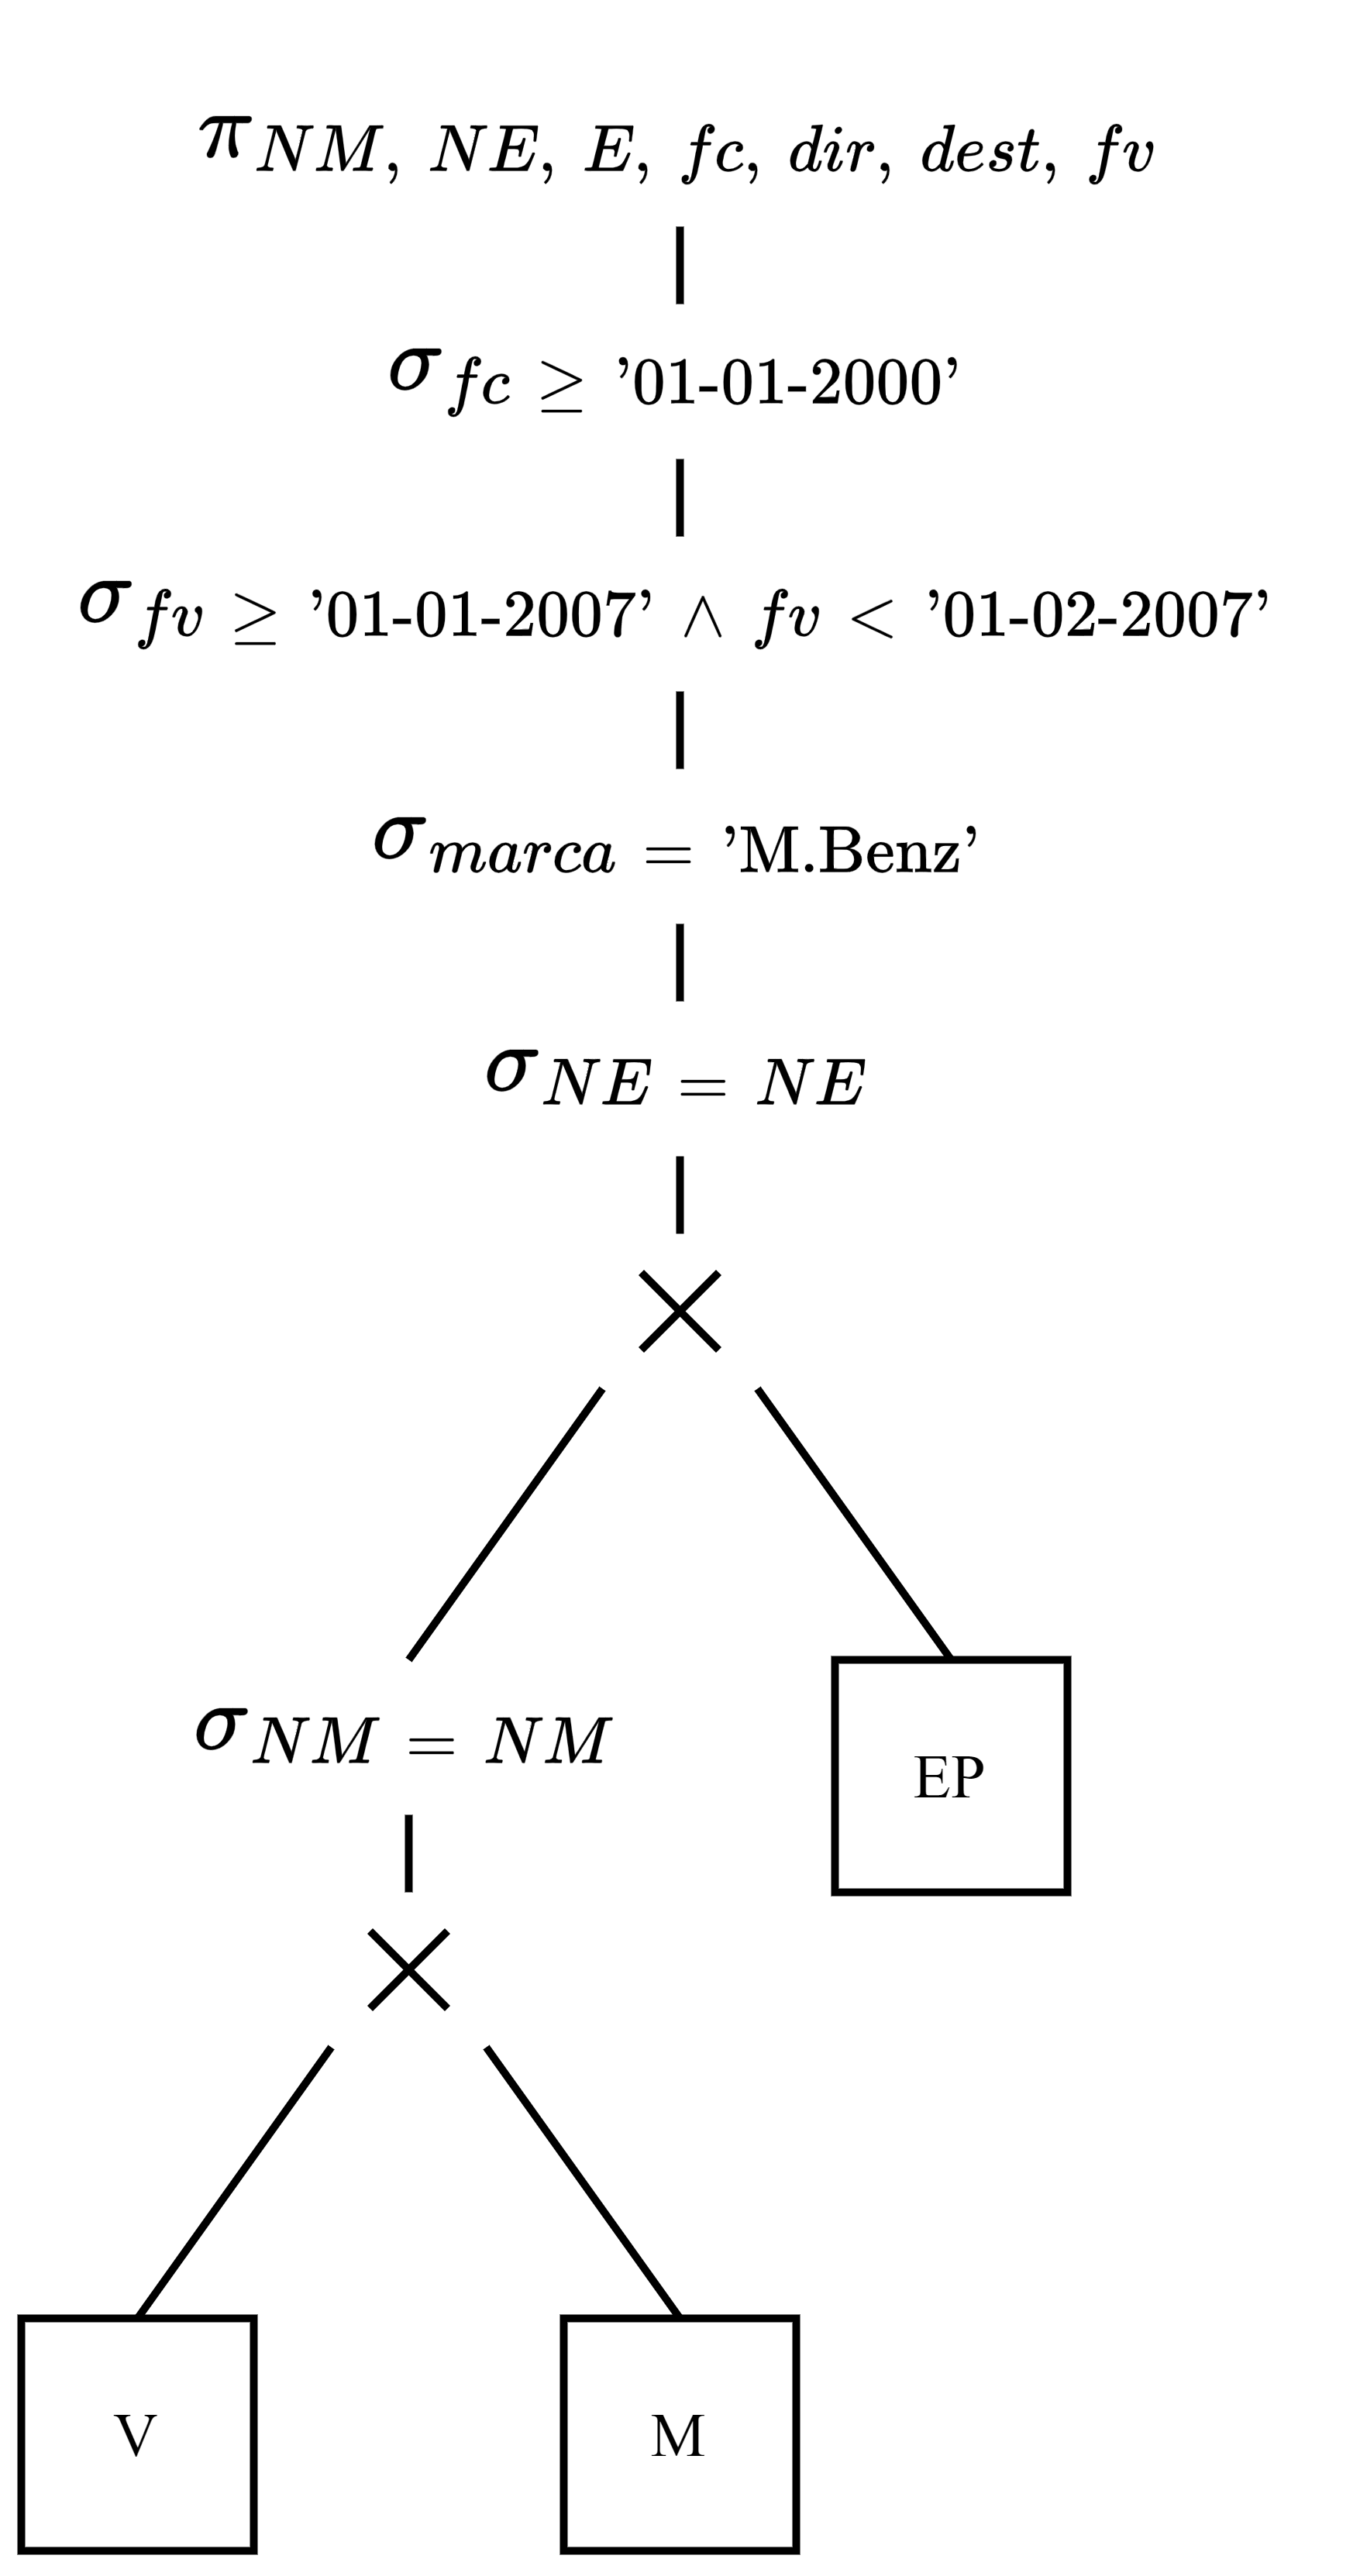
\includegraphics[width=0.35\textwidth]{img/E6-Paso-3.png}
        \end{figure}

        \item Cambio $\times$ por $\Join$.
        \begin{figure}[H]
            \centering
            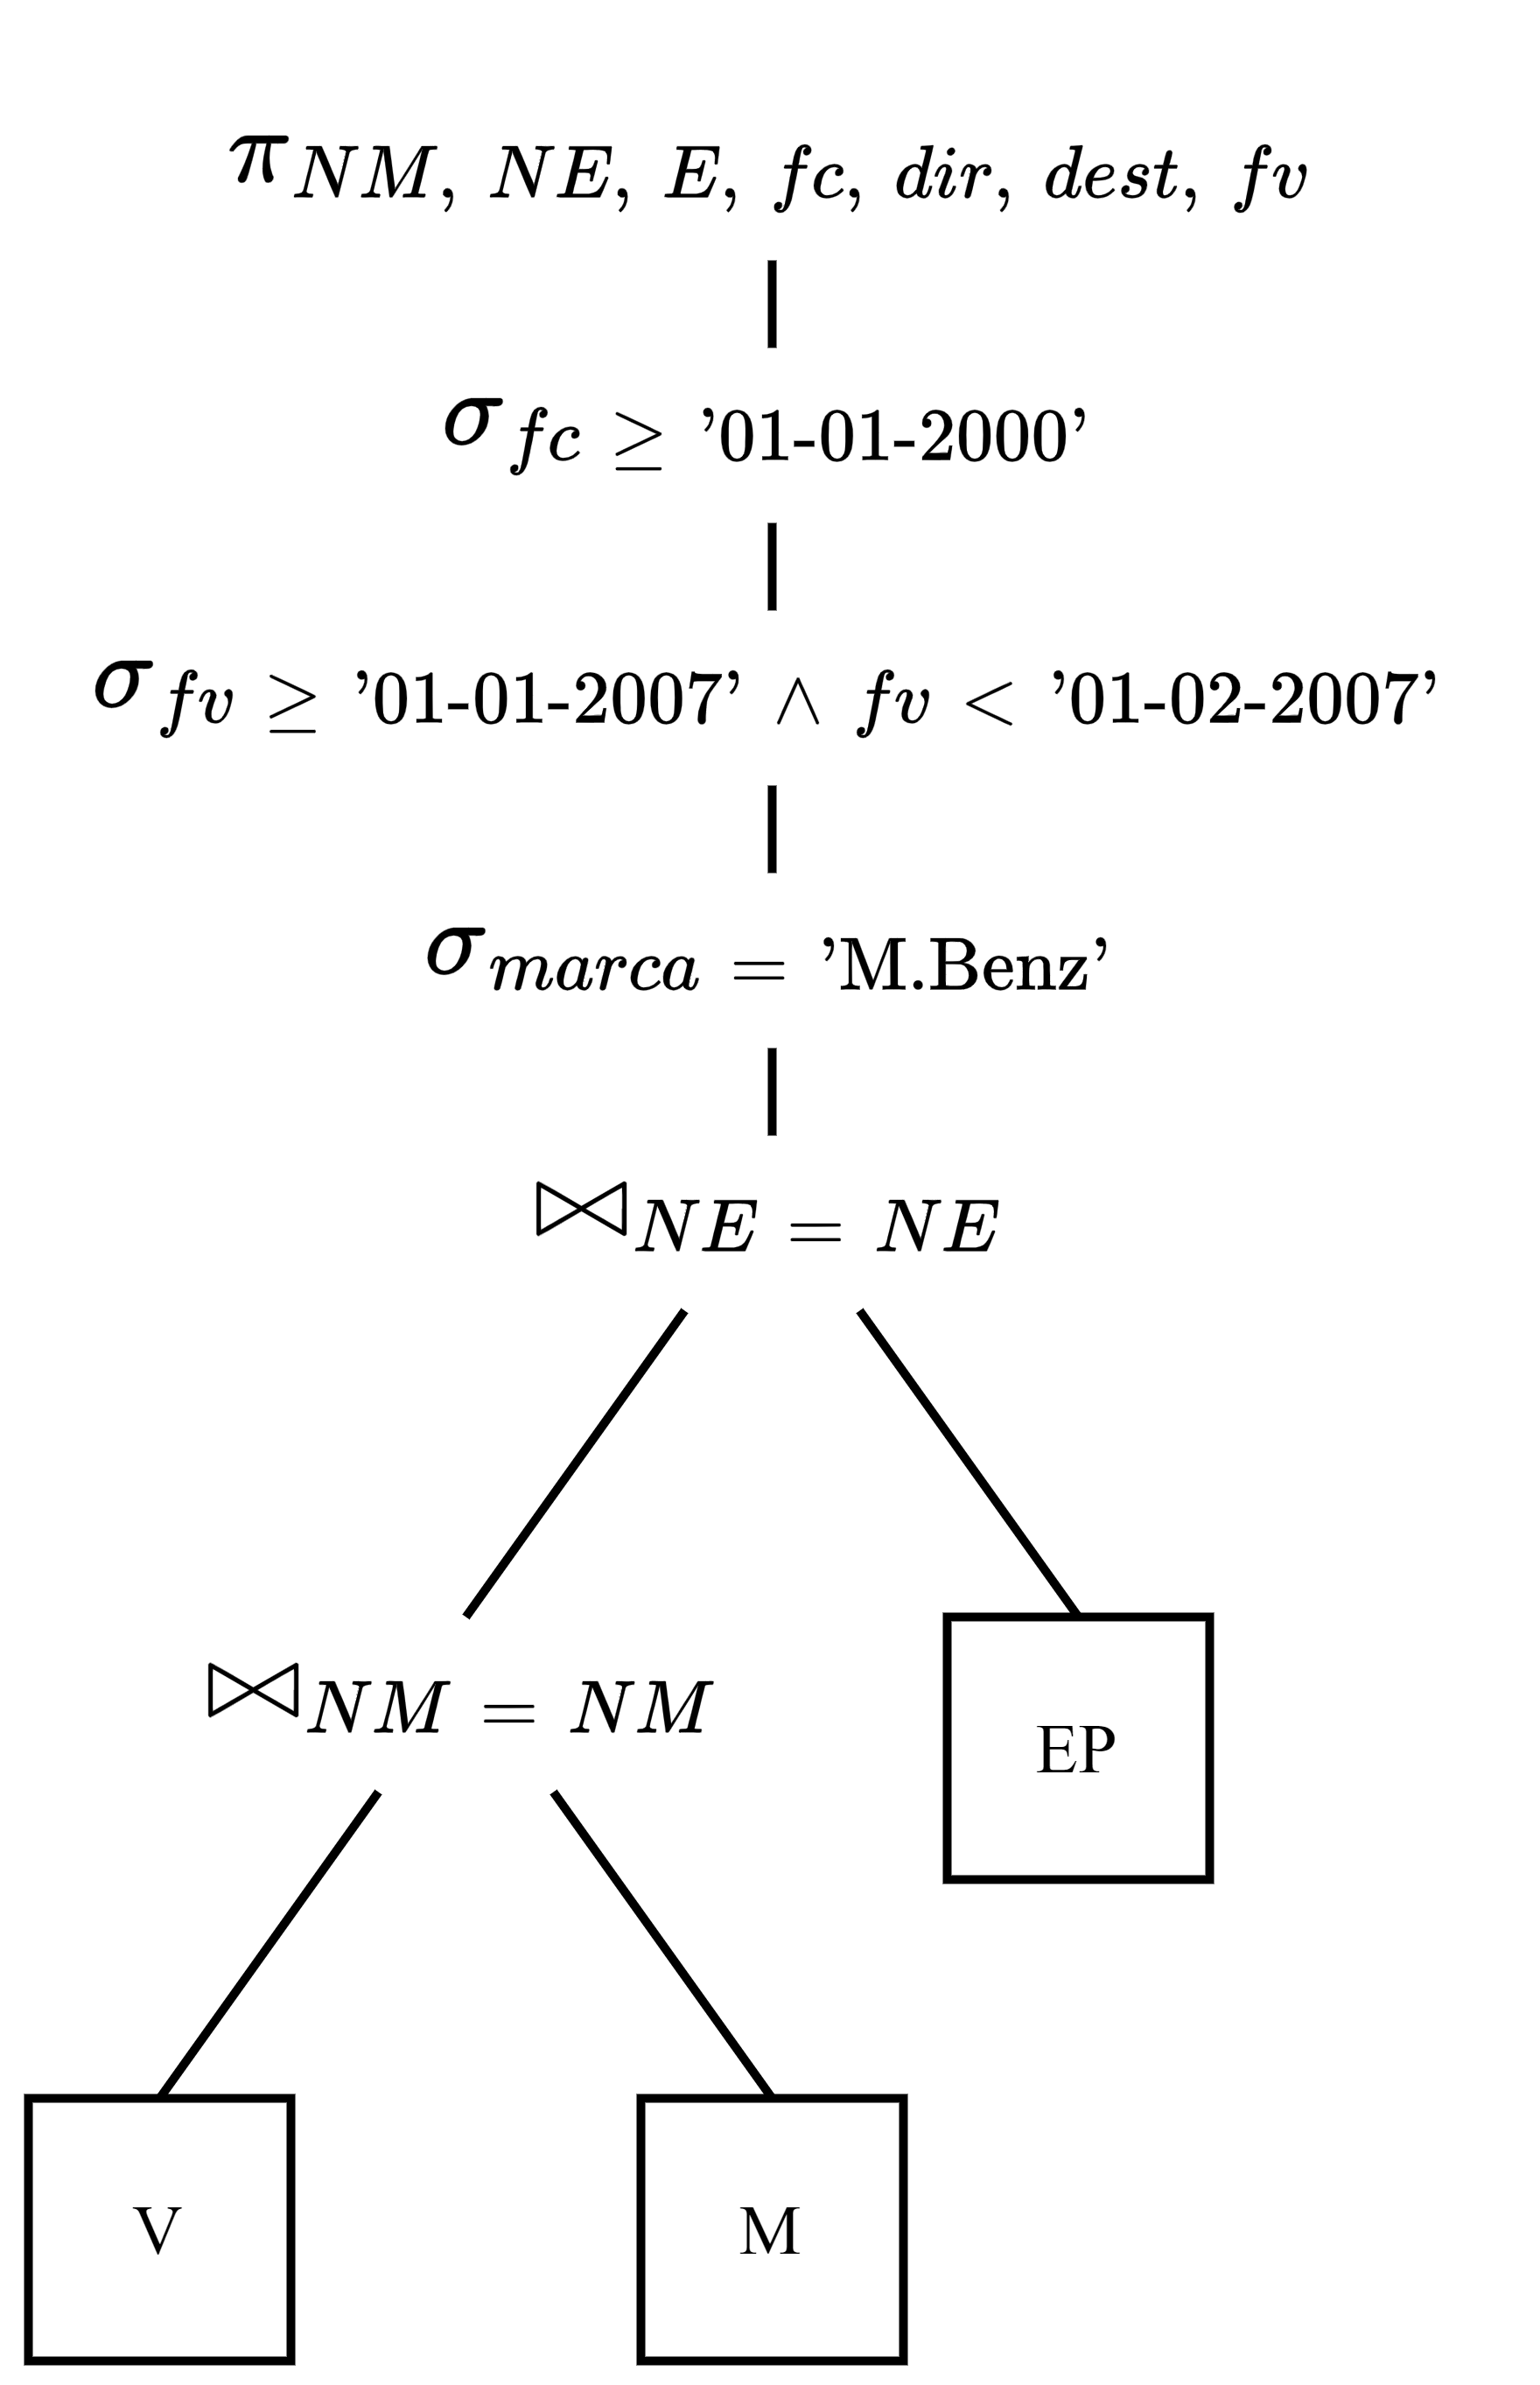
\includegraphics[width=0.4\textwidth]{img/E6-Paso-4.png}
        \end{figure}

        \item Bajar el resto de seleciones a tablas.
        \begin{figure}[H]
            \centering
            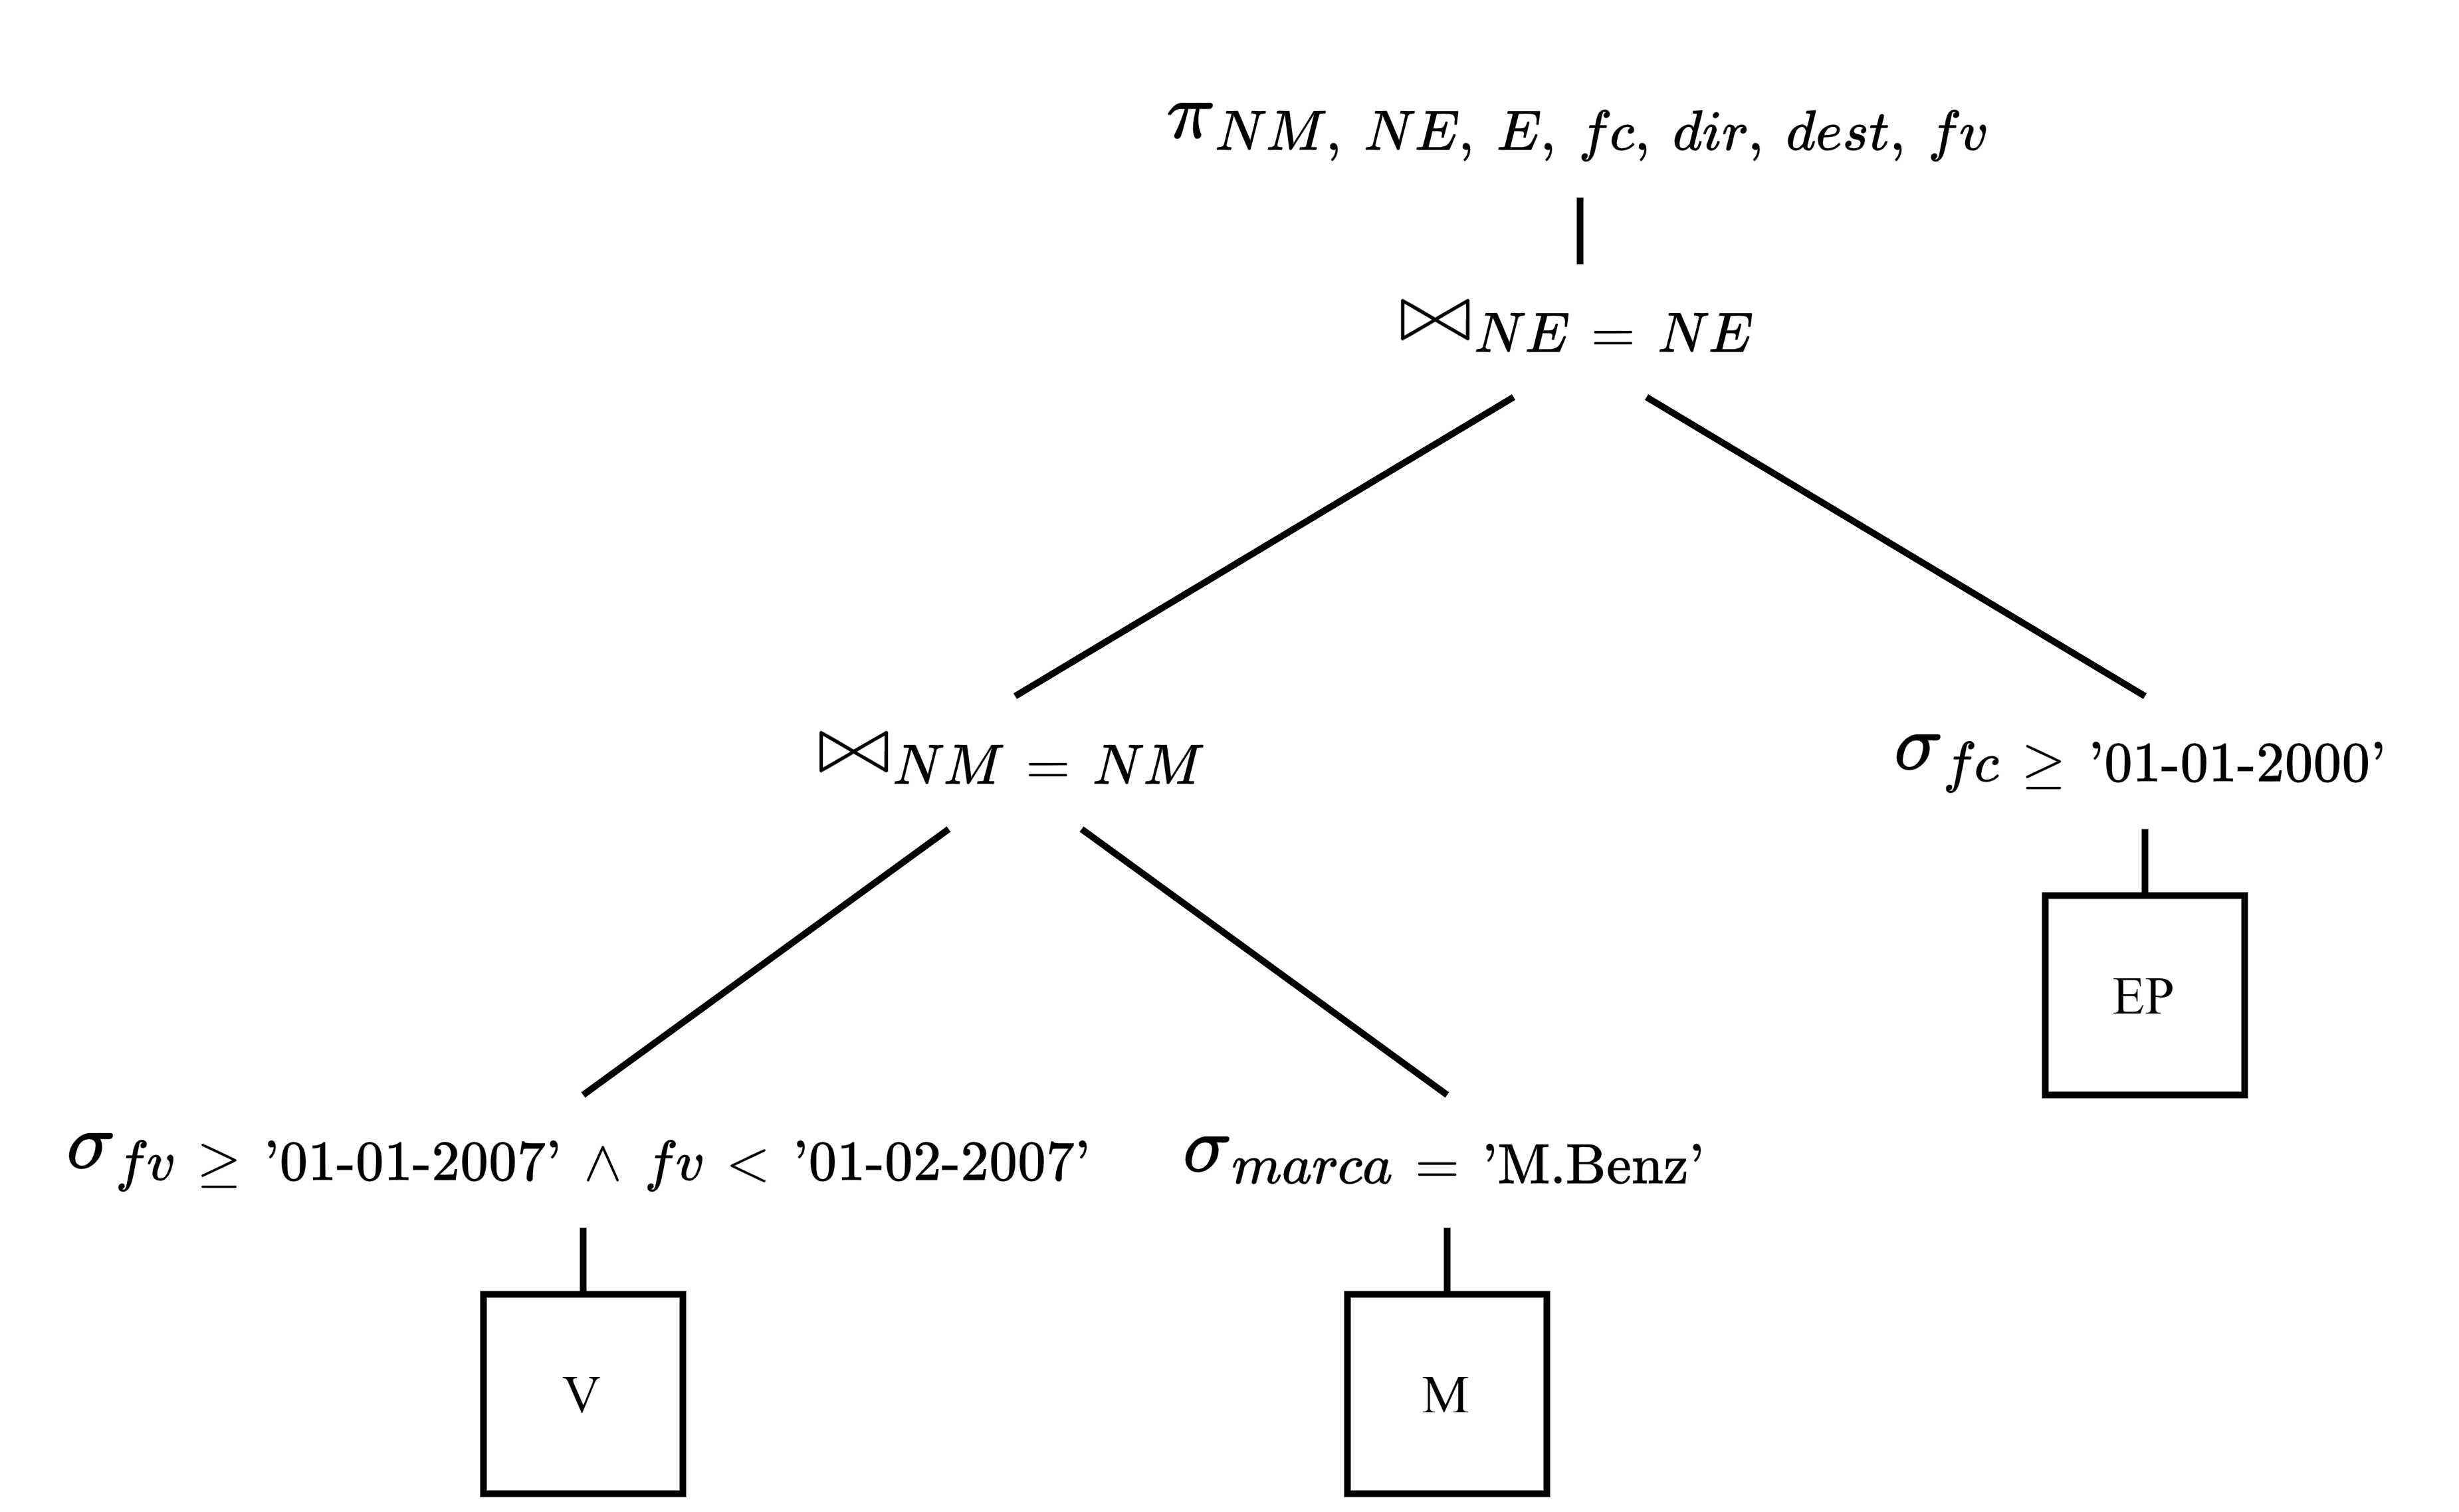
\includegraphics[width=\textwidth]{img/E6-Paso-5.png}
        \end{figure}

        \newpage
        \item Proyectar los atributos necesarios.
        \begin{figure}[H]
            \centering
            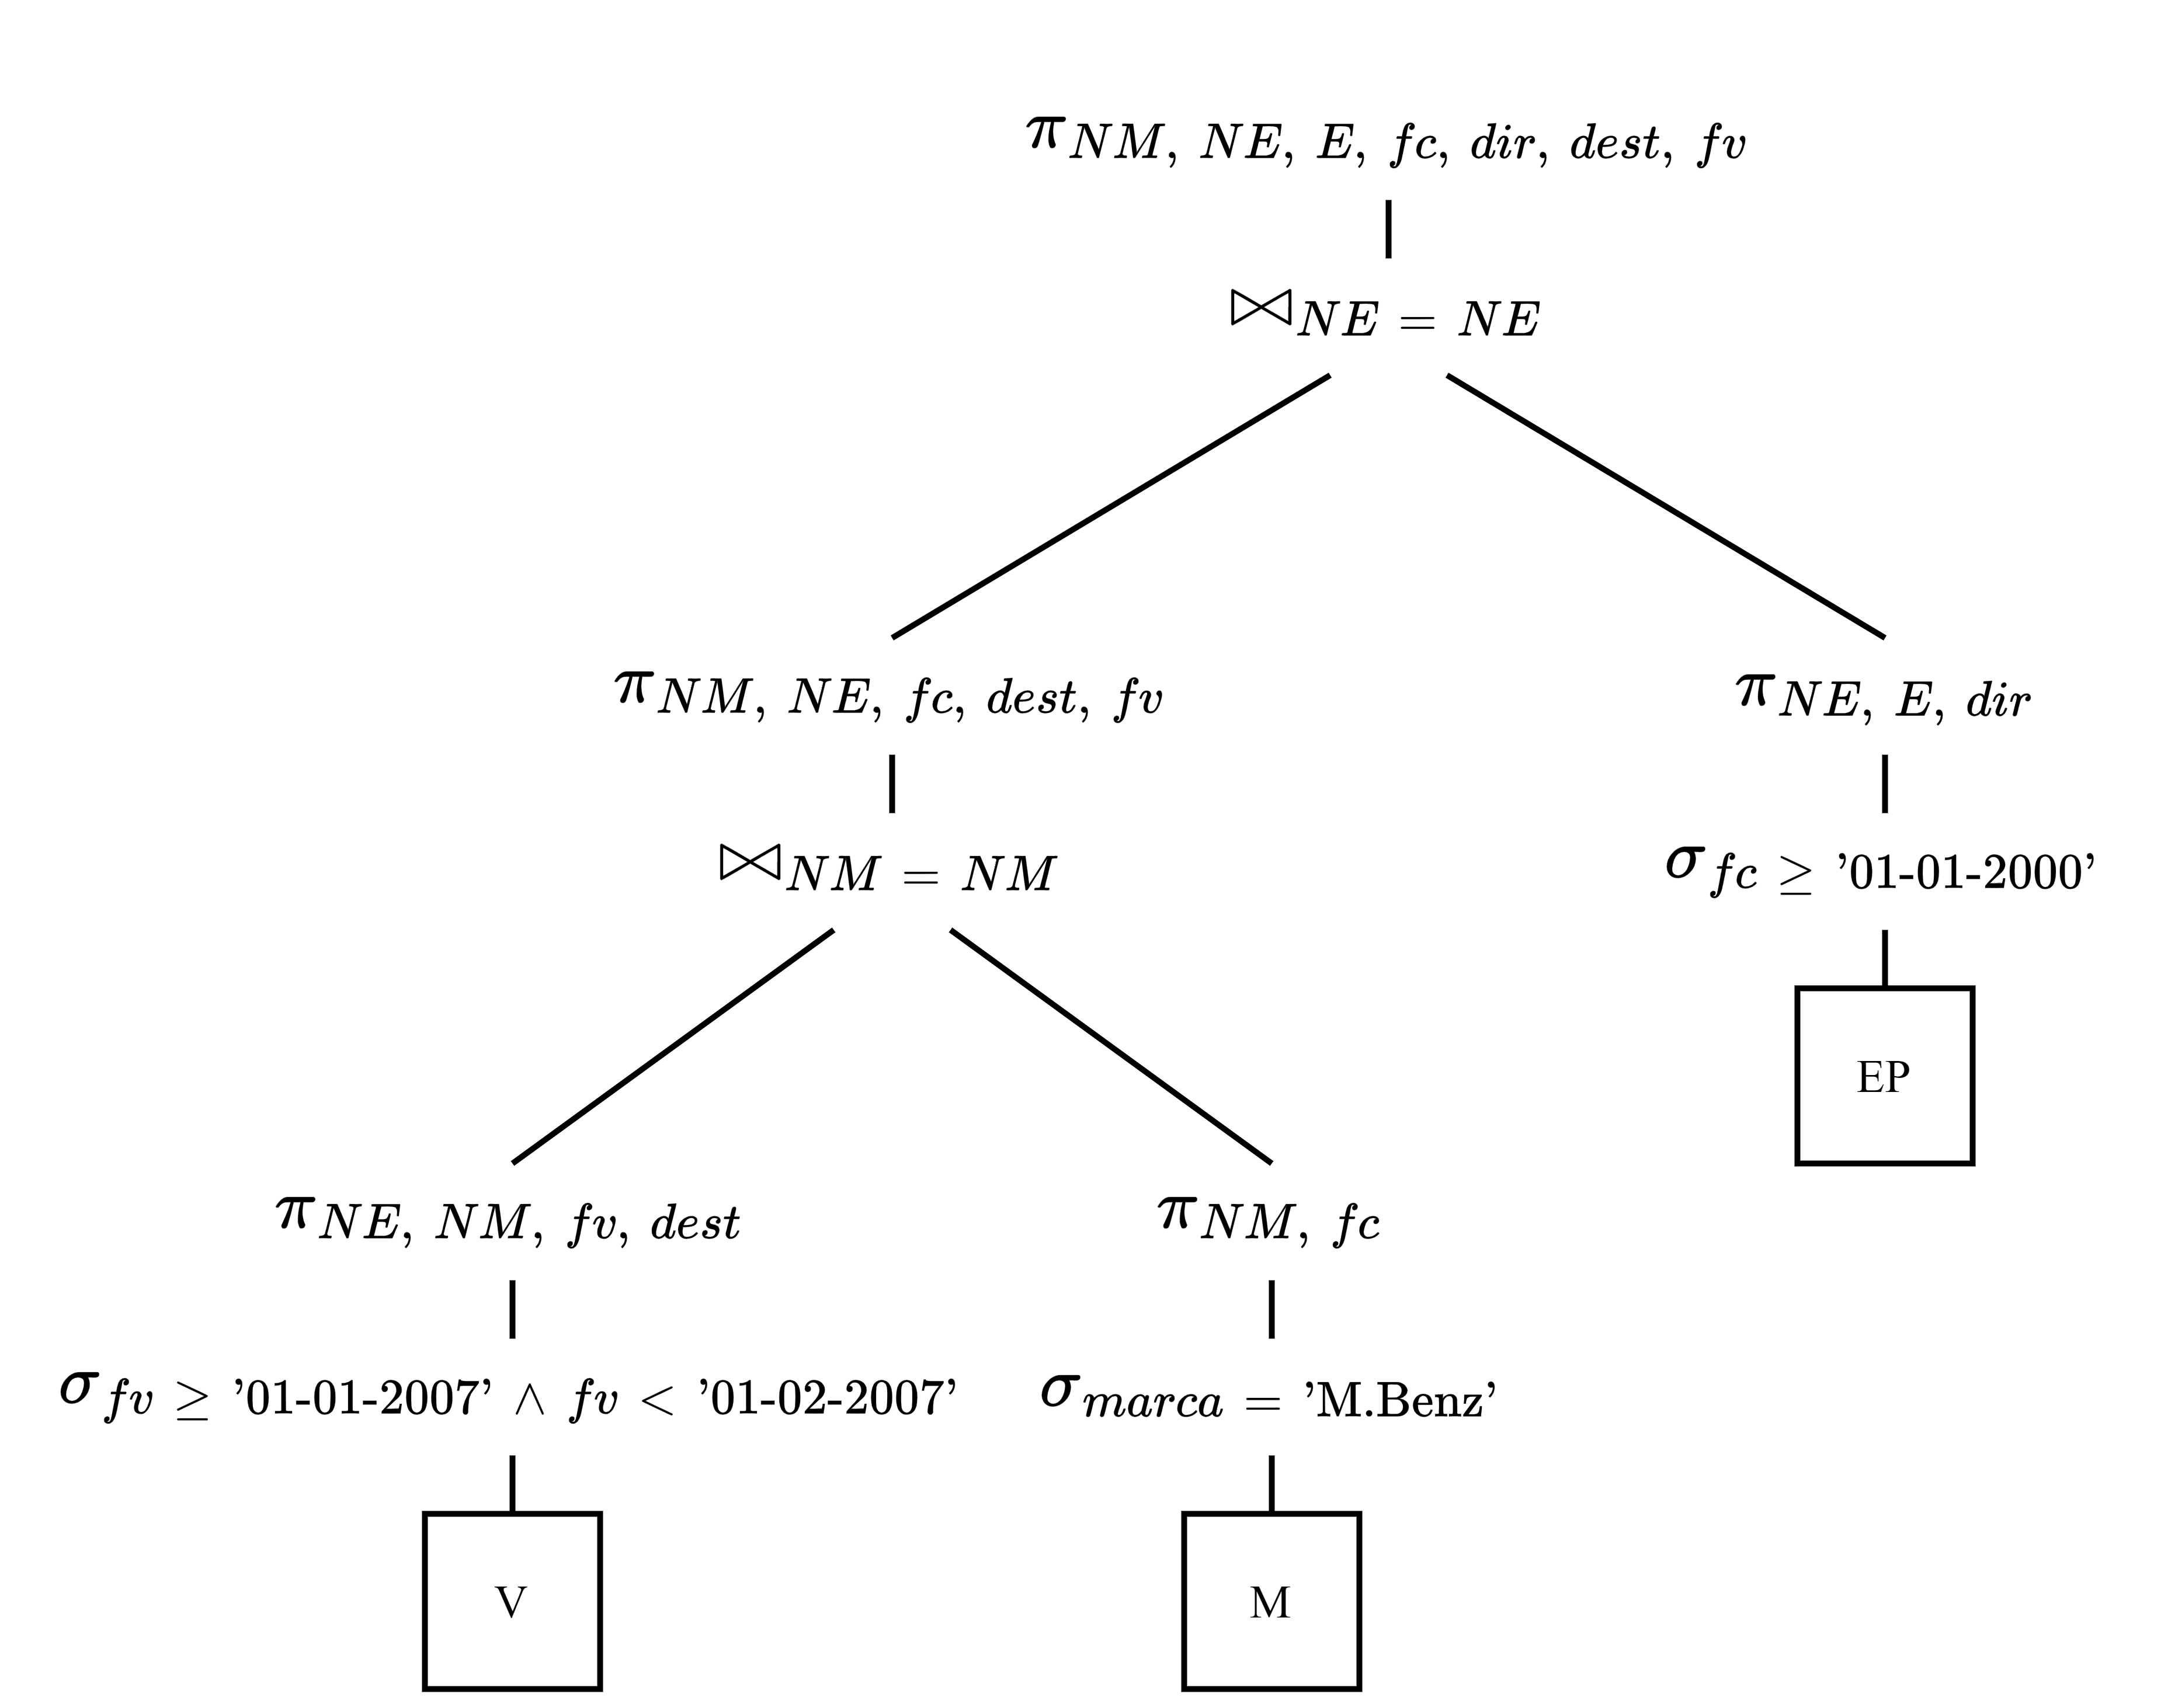
\includegraphics[width=\textwidth]{img/E6-Paso-6.png}
        \end{figure}
    \end{enumerate}
\end{itemize}
\newpage
\subsection{Clase 19 de junio, 2024}
Sean las tablas:
\begin{itemize}
    \item Variedades(\textbf{idvar}, nombre, prog2, prog1)
    \item Predios(\textbf{idpredio}, nombrepredio, comuna, superficie)
    \item Siembra(\textbf{idpredio}, \textbf{idvar}, hasem, rdto, a\~no)
\end{itemize}
\begin{enumerate}
    \item Listar los nombres de las variedades sembradas en el predio \hlcolor{Celeste!50}{idpredio = 10} y que el \hlcolor{Celeste!50}{a\~no 2015 tuvieron rendimiento mayor a $60qq/ha$}.
    \begin{itemize}
        \item SQL.
        \begin{verbatim}
SELECT V.nombre
FROM Variedades V,
     Predios P,
     Siembra S,
WHERE V.idvar = S.idvar
AND S.idpredio = P.idpredio
AND P.idpredio = 10
AND S.año = 2015
AND S.rdto > 60;
        \end{verbatim}

        \item Algebra Relacional.
        \begin{align*}
            \scalebox{1.5}{$\pi$}_{\text{nombre}} (
                \scalebox{1.5}{$\sigma$}_{
                    \scalebox{0.8}{
                        $\begin{array}{l}
                            \text{idvar} = \text{idvar} \; \wedge \\
                            \text{idpredio} = \text{idpredio} \; \wedge \\
                            \text{idpredio} = 10 \; \wedge \\
                            \text{a\~no} = 2015 \; \wedge \\
                            \text{rdto} > 60
                        \end{array}$
                    }
                } (
                    \text{Variedades}_{\scalebox{1.3}{$\Join$}} (
                        \text{Predios}_{\scalebox{1.3}{$\Join$}} \text{Siembra}
                    )
                )
            )
        \end{align*}
        
        \newpage
        \item Arbol Canonico.
        \begin{figure}[H]
            \centering
            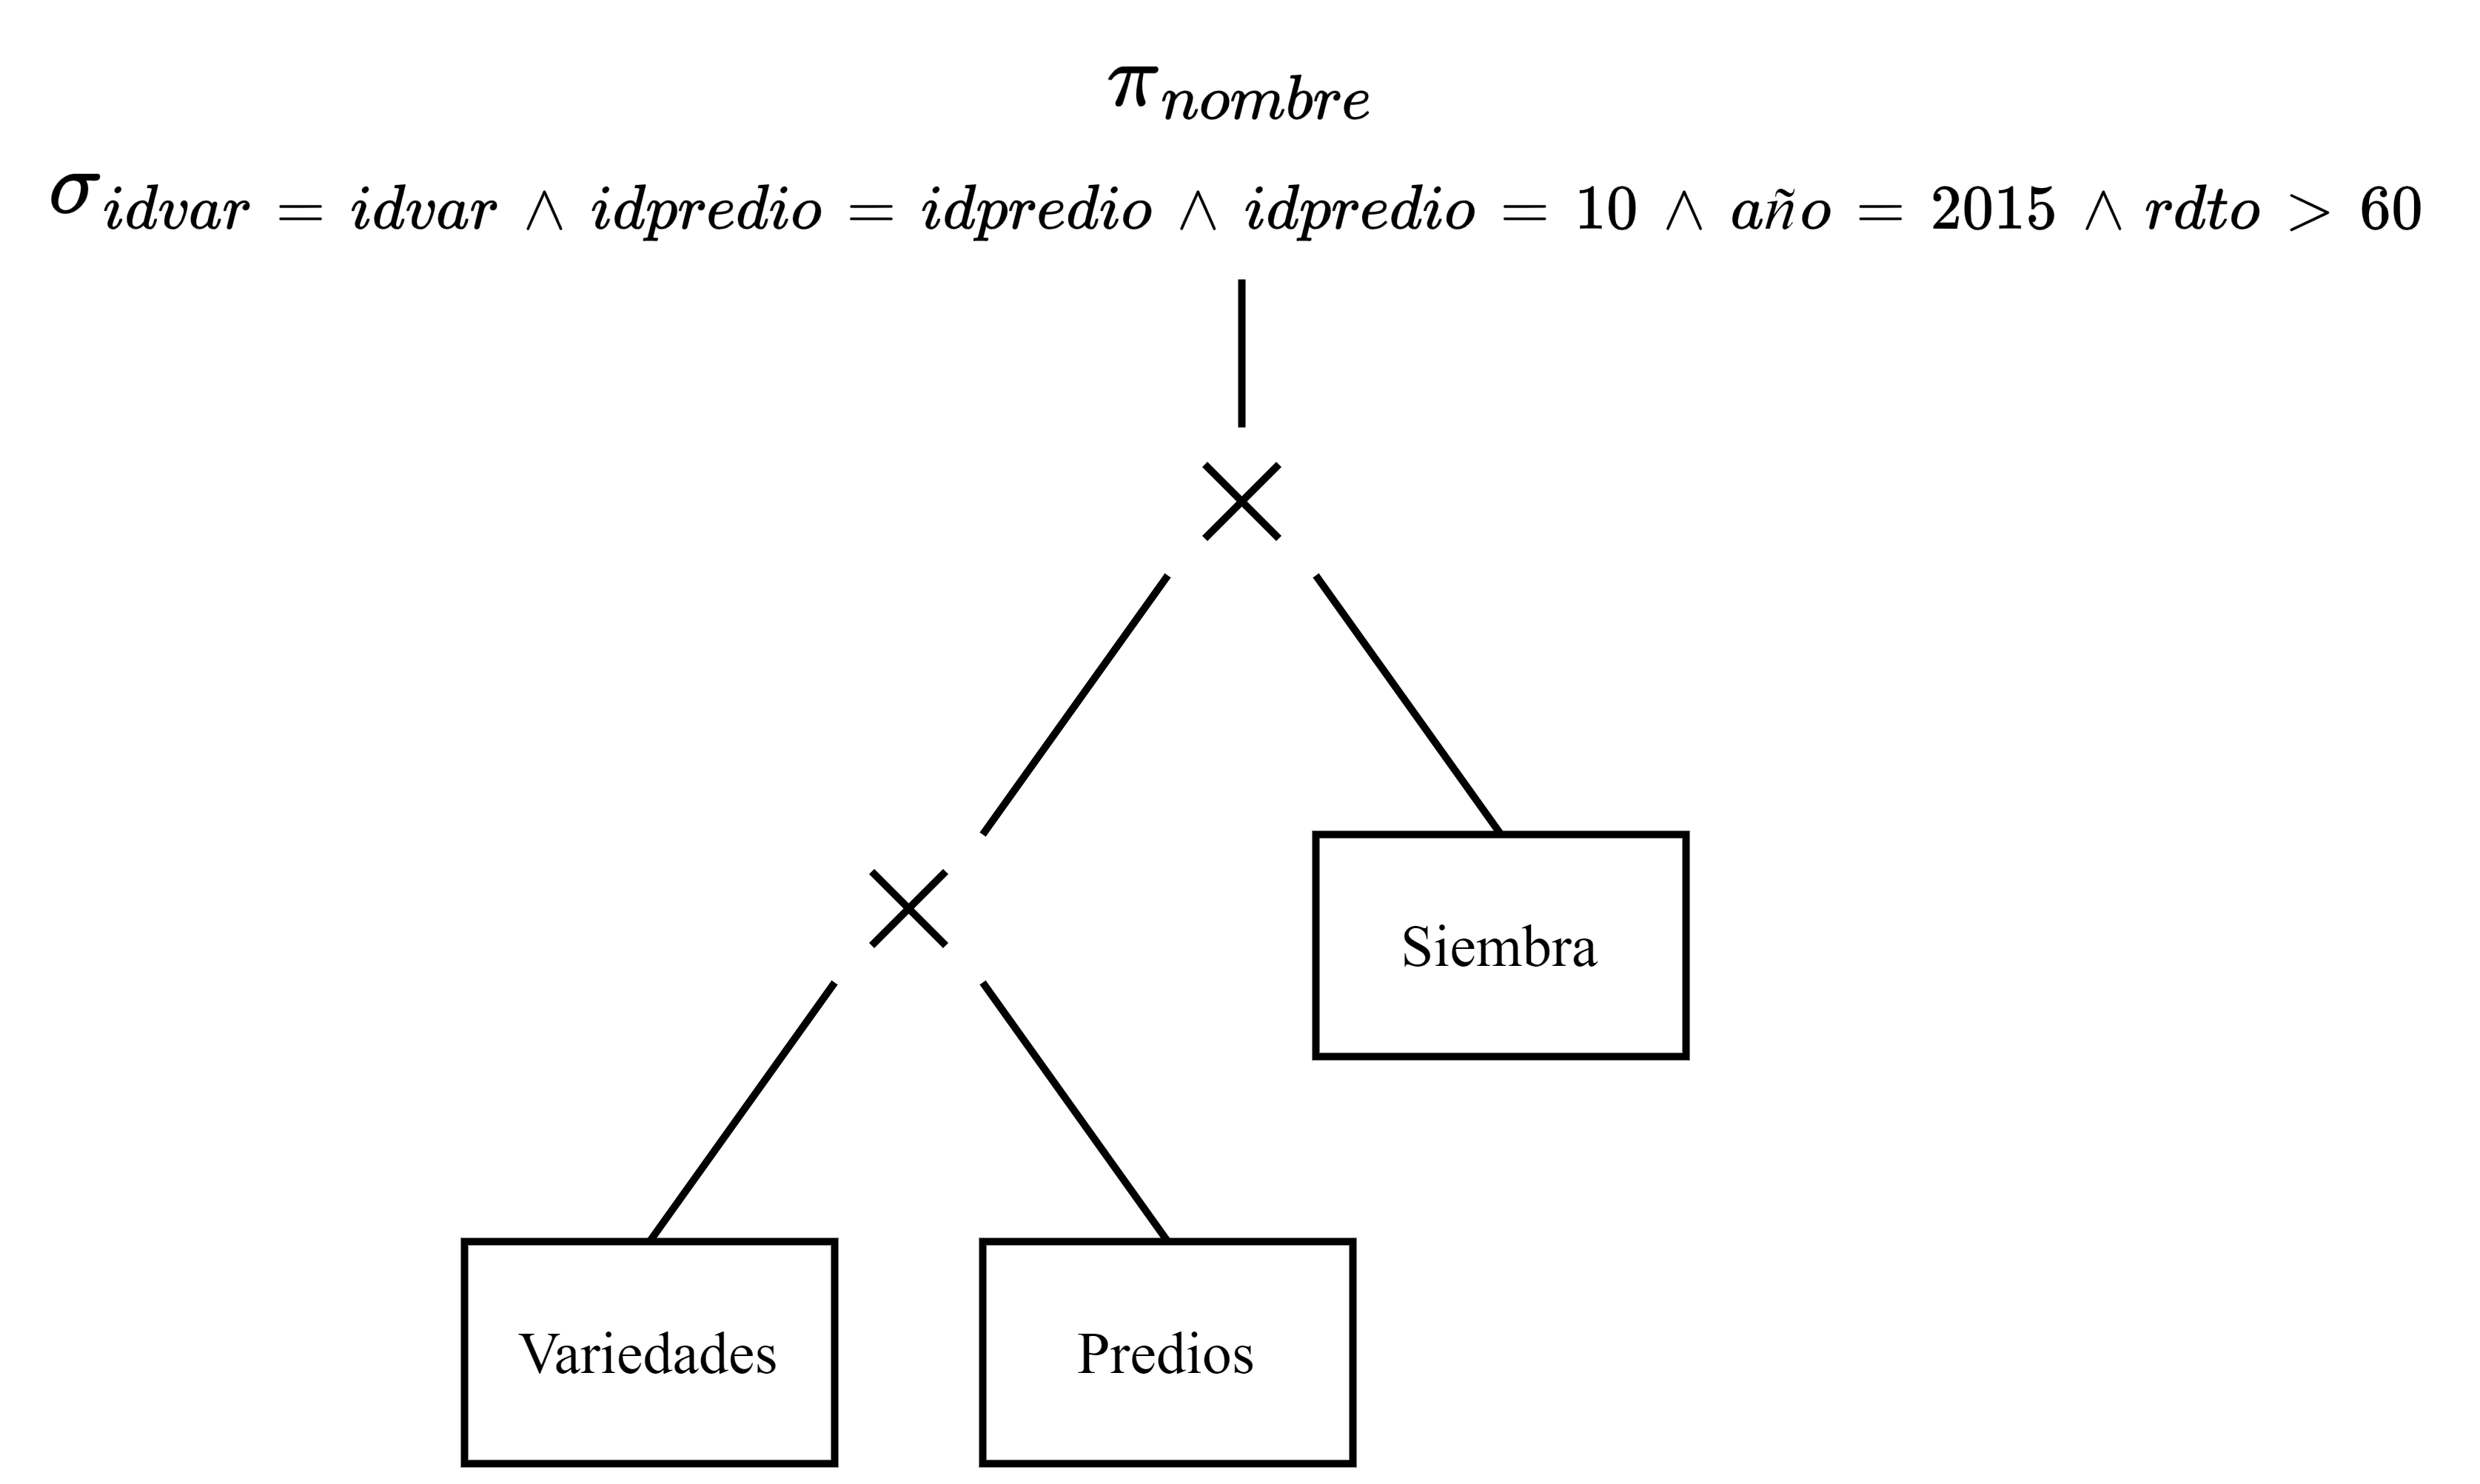
\includegraphics[width=0.7\textwidth]{img/E1-Canonico.png}
        \end{figure}

        \item Optimizaci\'on.
        \begin{enumerate}
            \item Separar las selecciones.
            \begin{figure}[H]
                \centering
                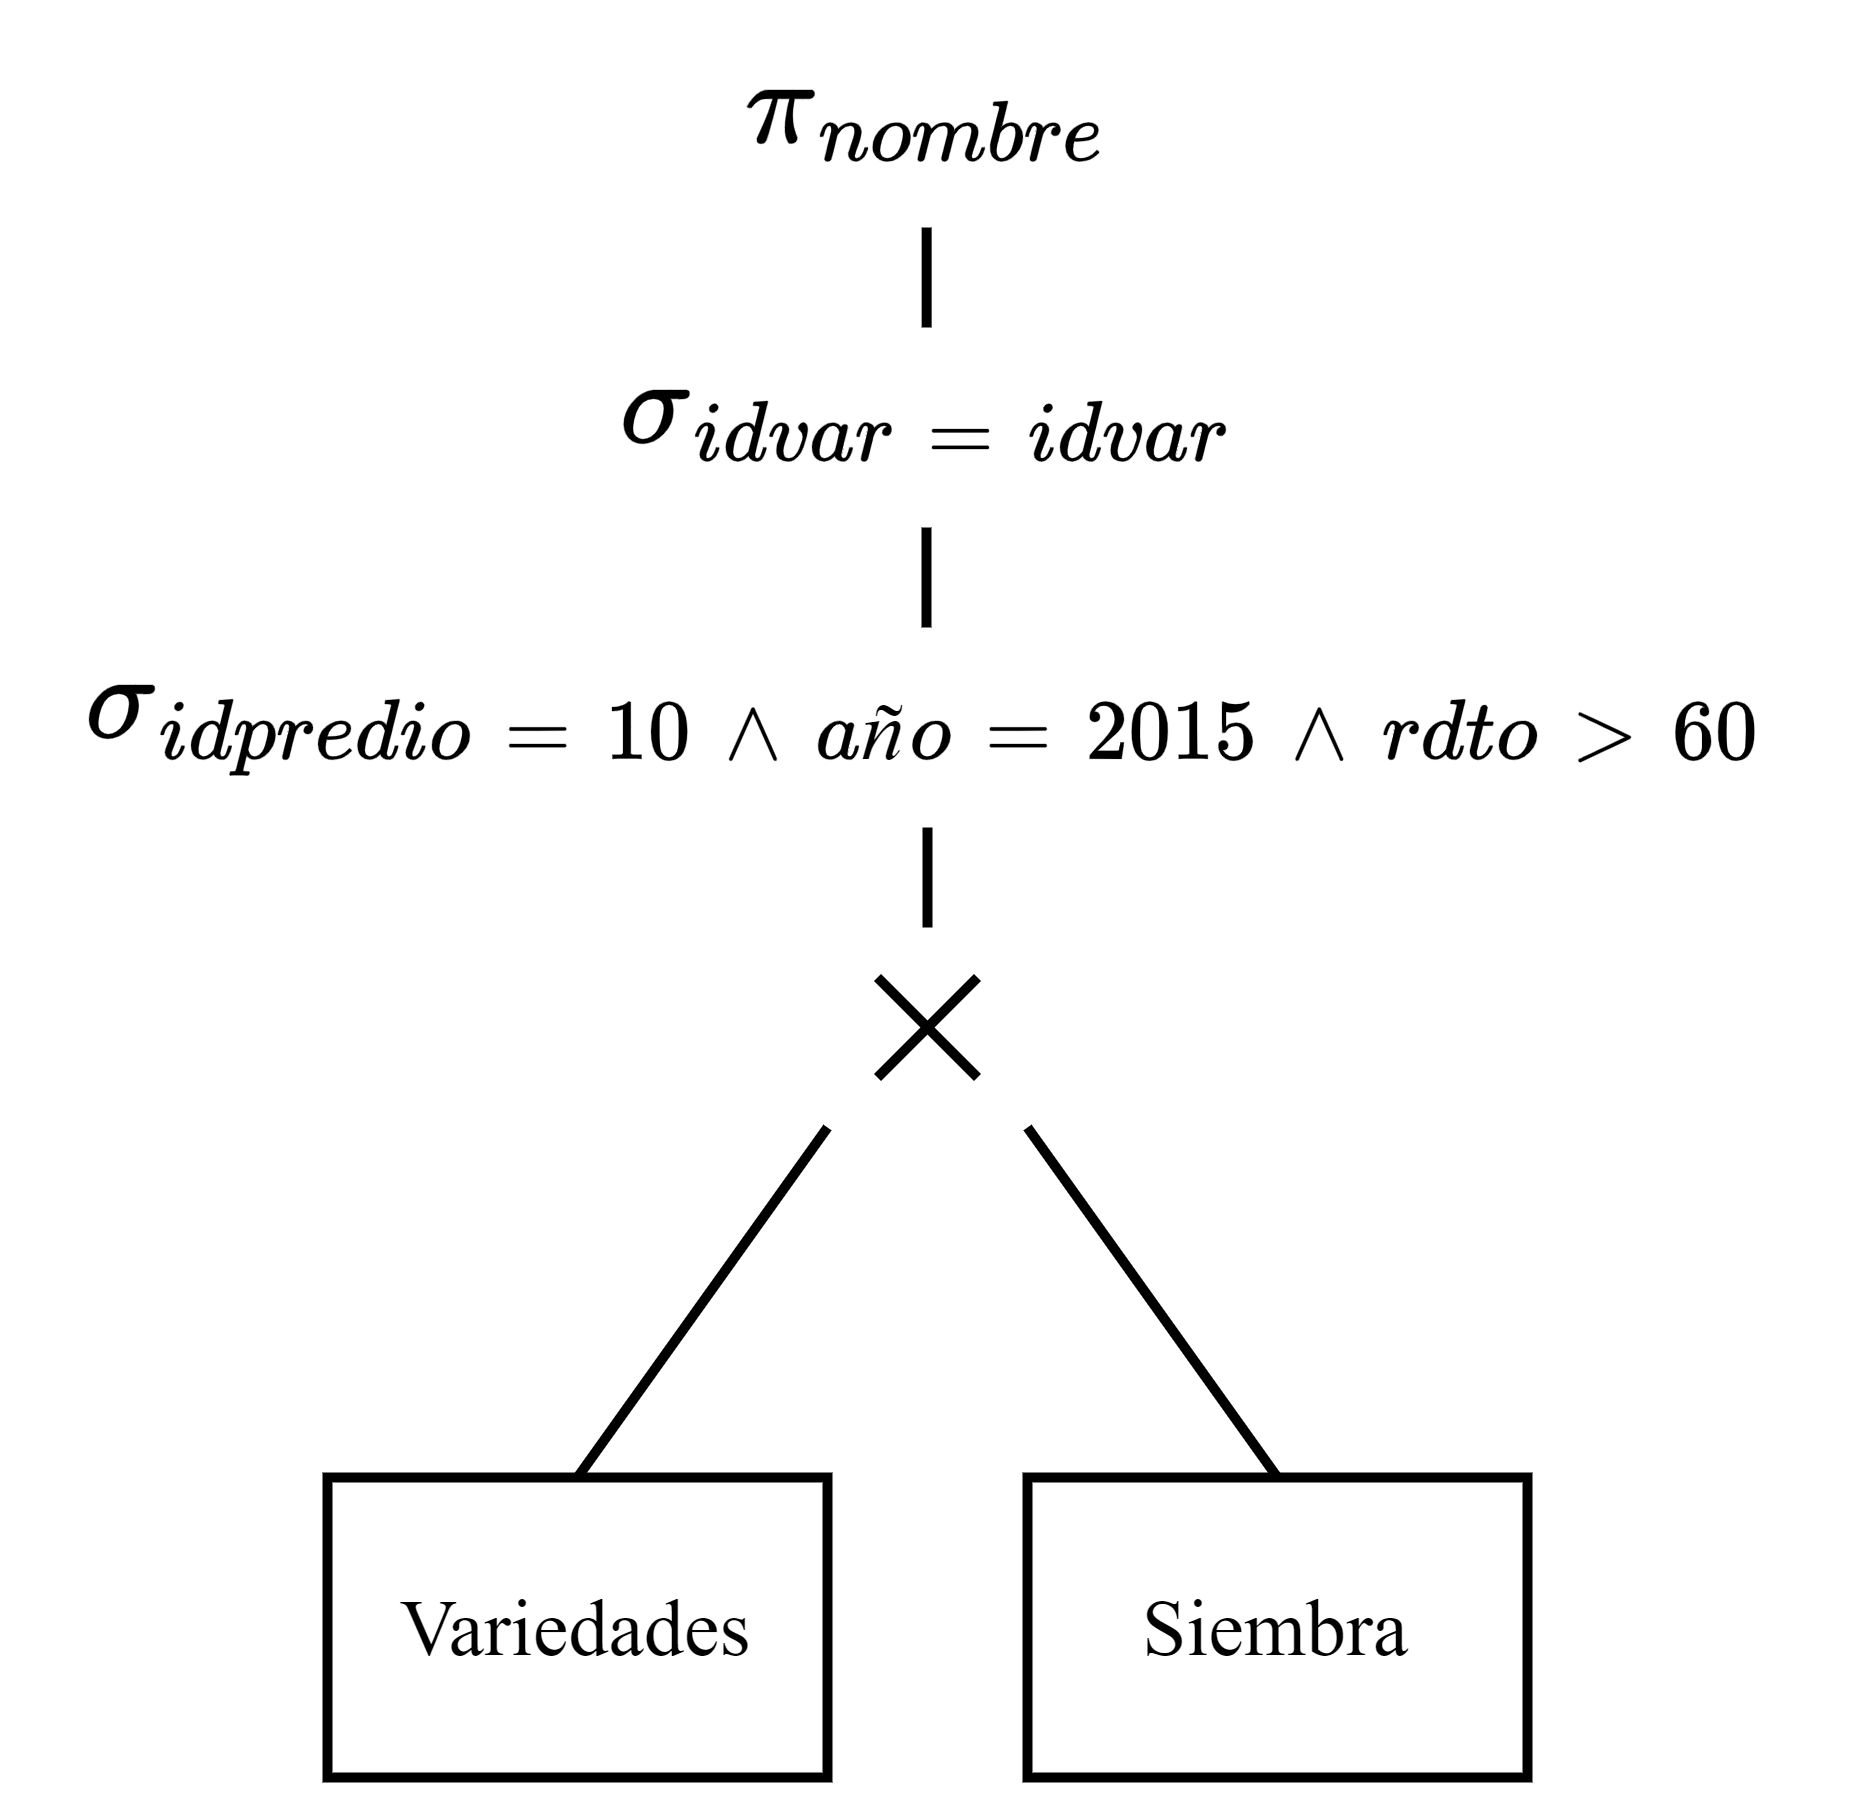
\includegraphics[width=0.4\textwidth]{img/E1-Paso-1.png}
            \end{figure}

            \newpage
            \item Permutar tablas si es necesario.
            \begin{figure}[H]
                \centering
                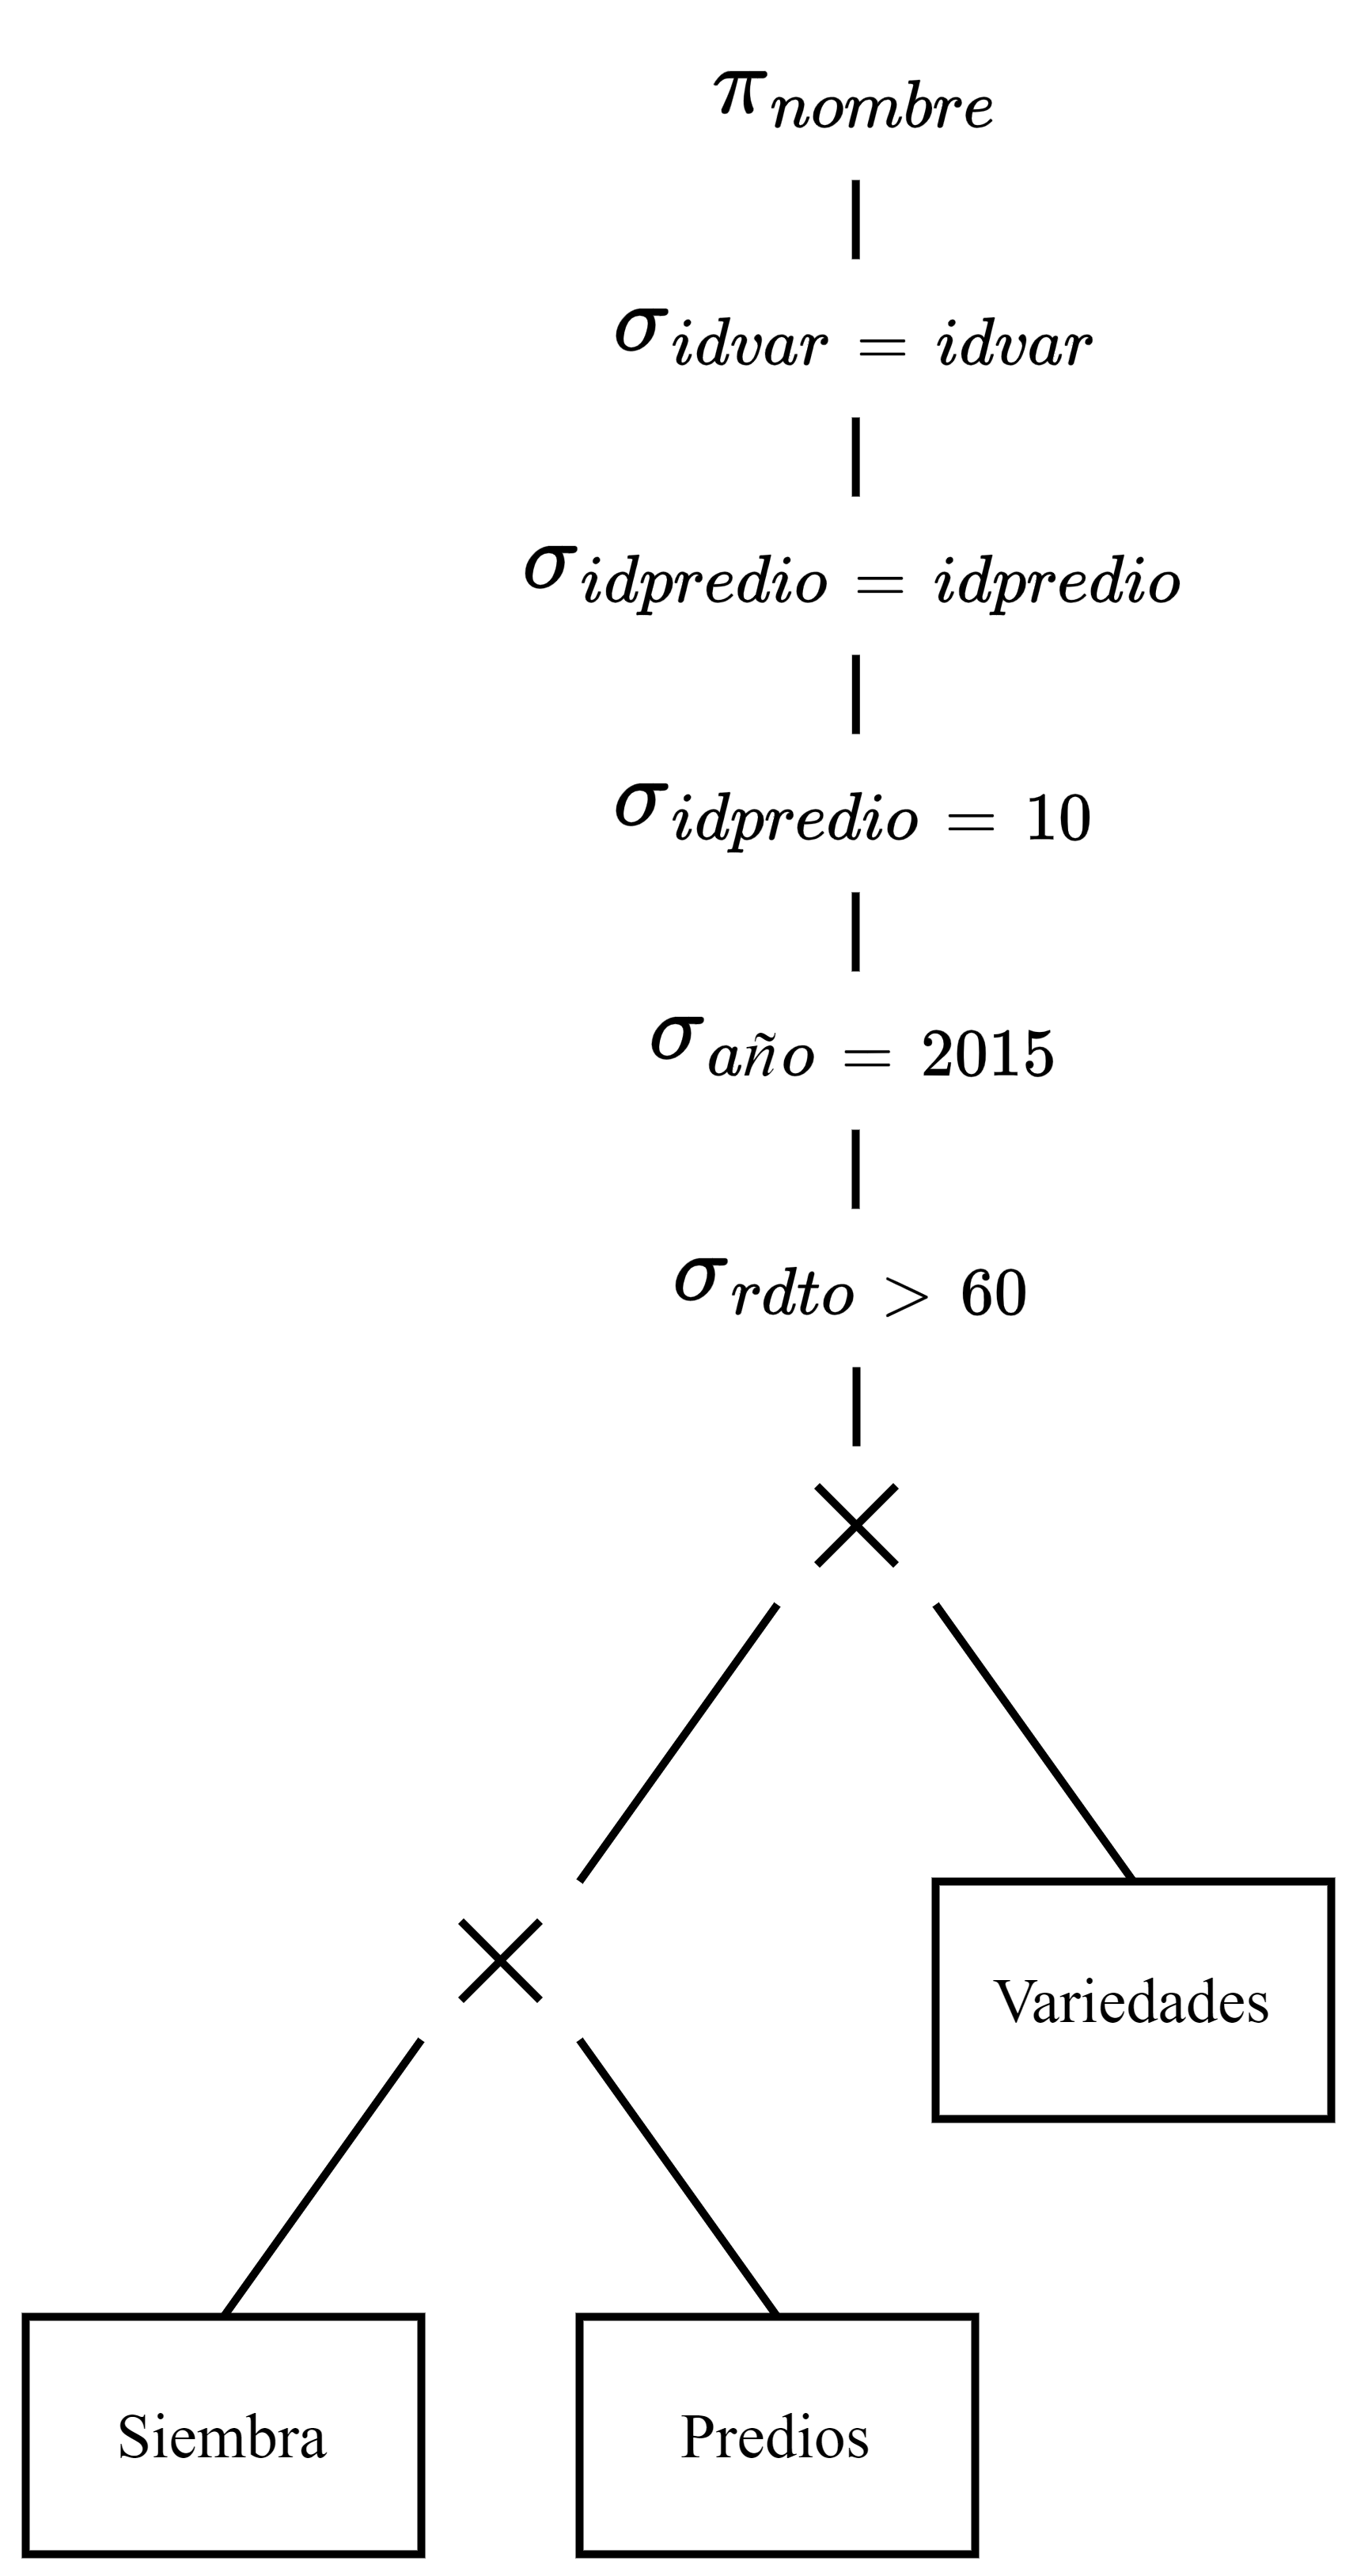
\includegraphics[width=0.4\textwidth]{img/E1-Paso-2.png}
            \end{figure}

            \item Bajar las seleciones que son $\times$ para $\Join$.
            \begin{figure}[H]
                \centering
                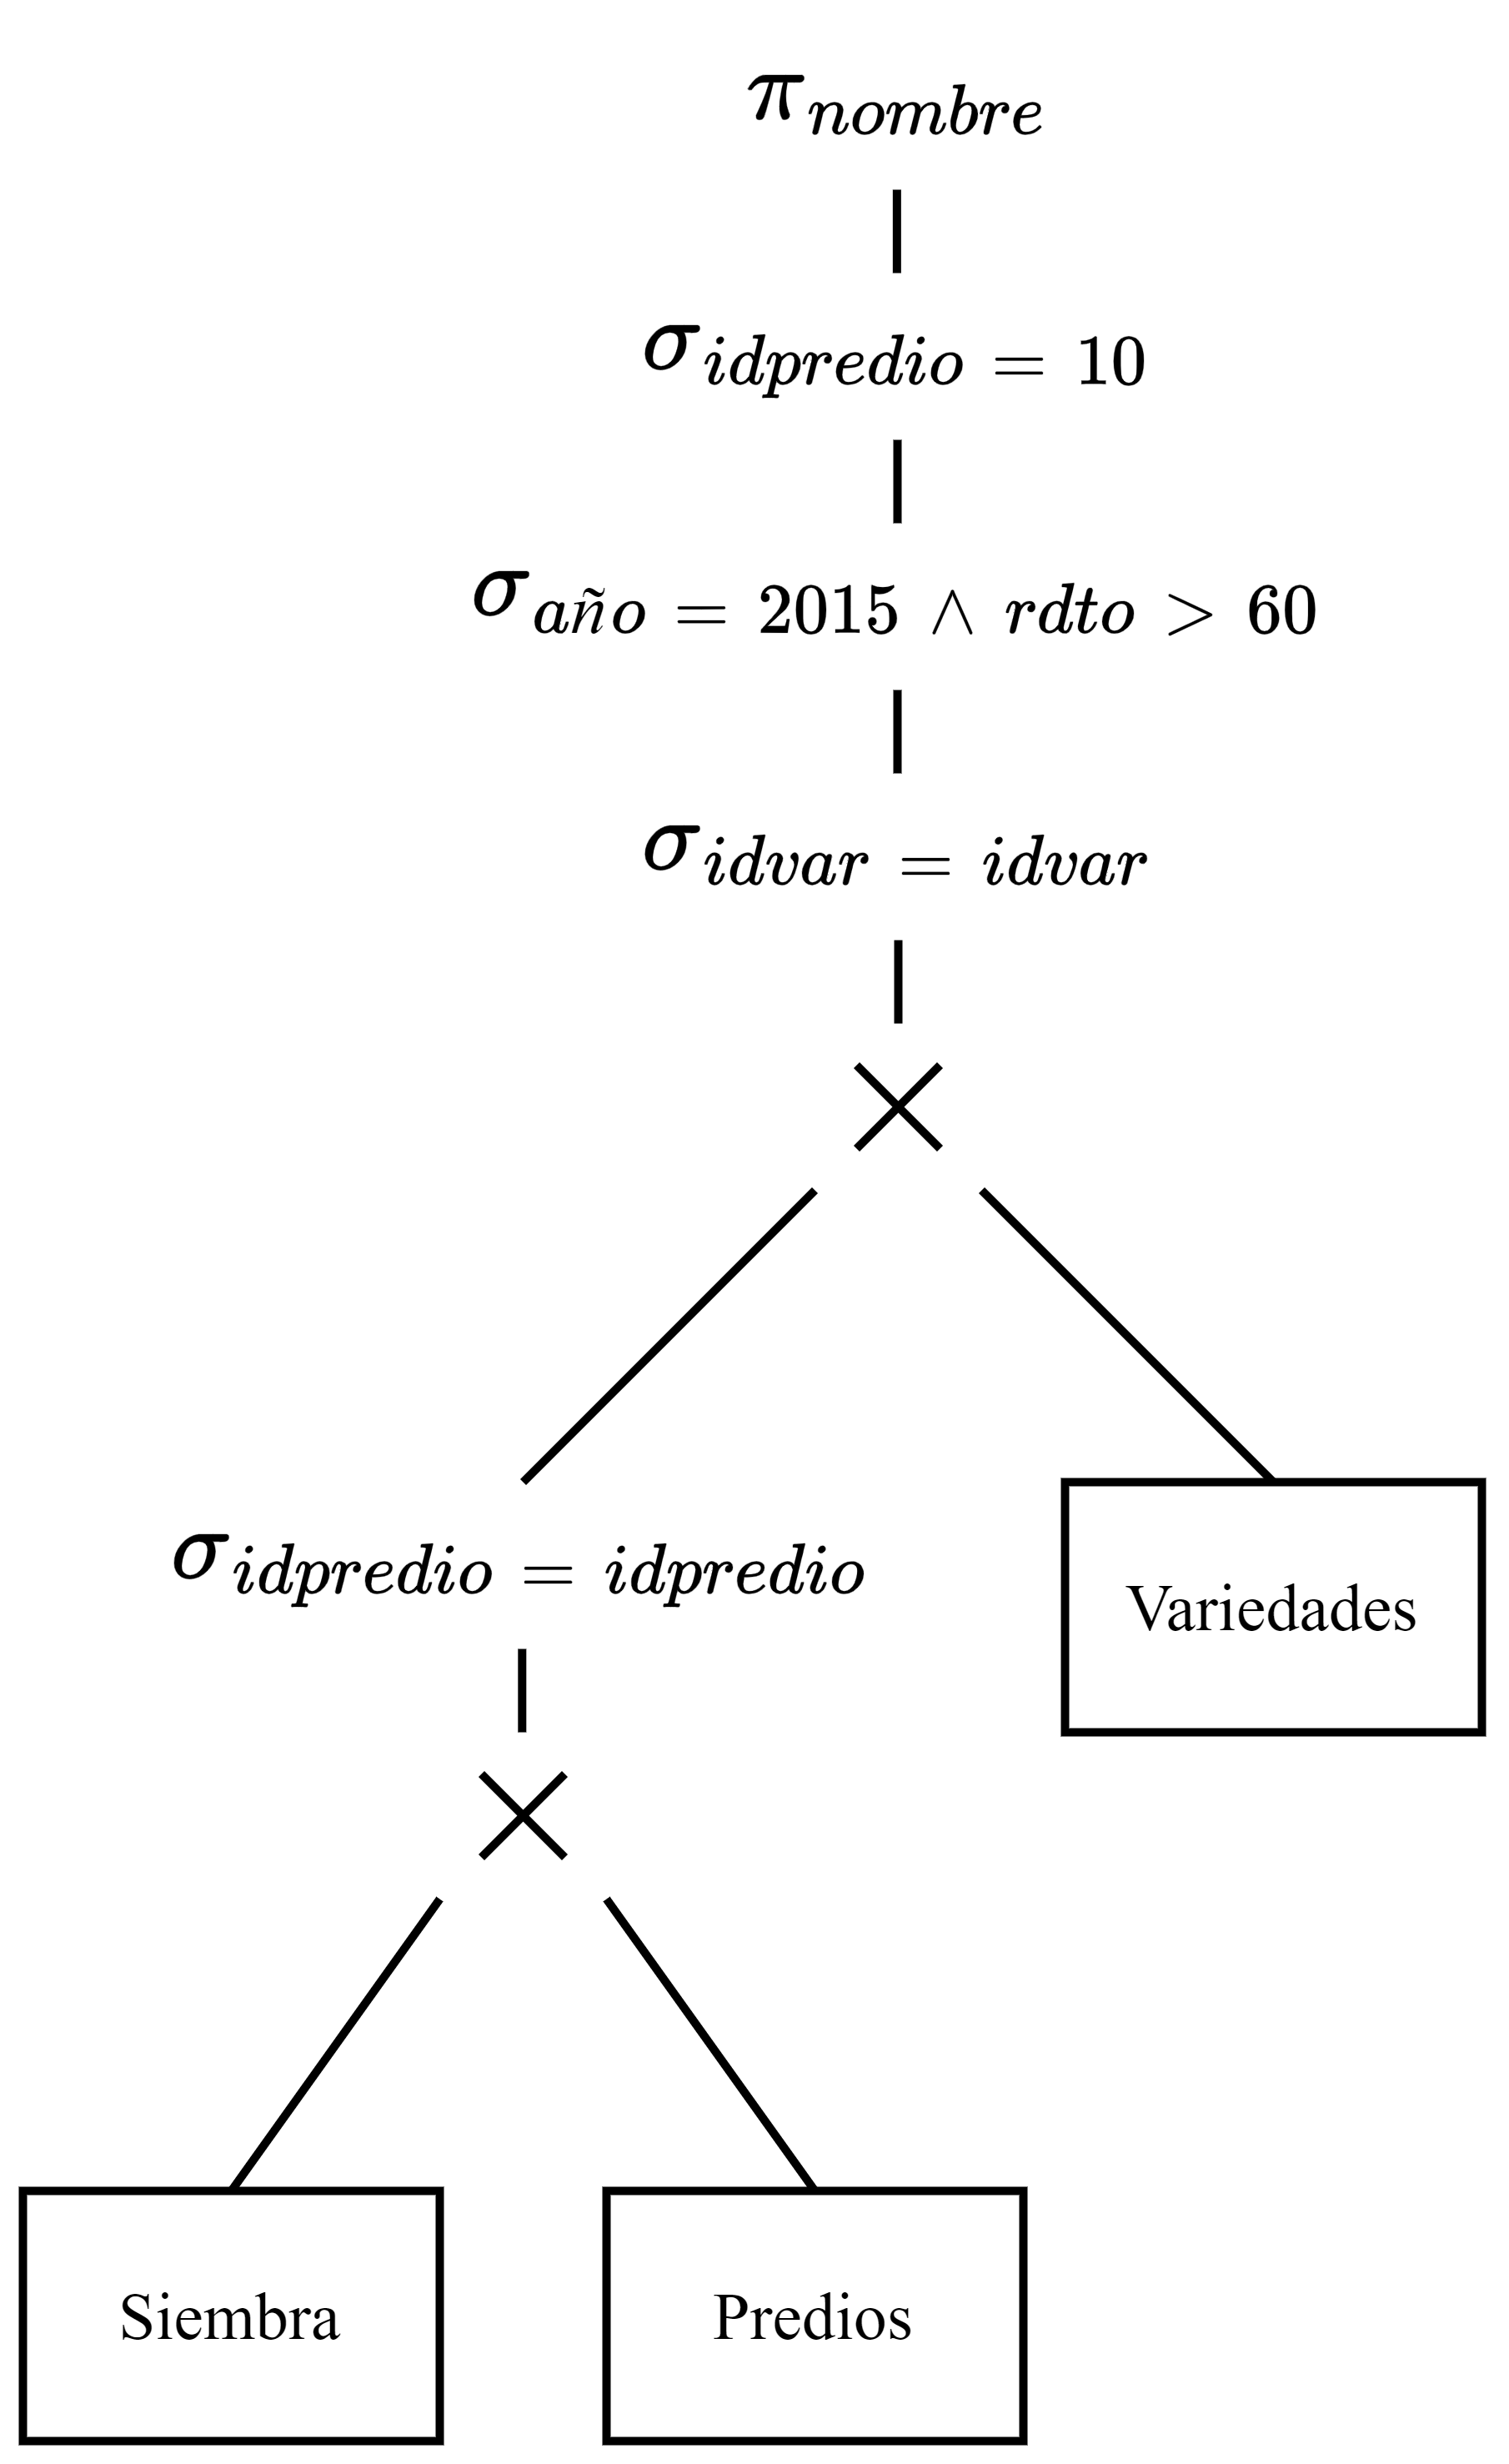
\includegraphics[width=0.4\textwidth]{img/E1-Paso-3.png}
            \end{figure}

            \item Cambio $\times$ por $\Join$.
            \begin{figure}[H]
                \centering
                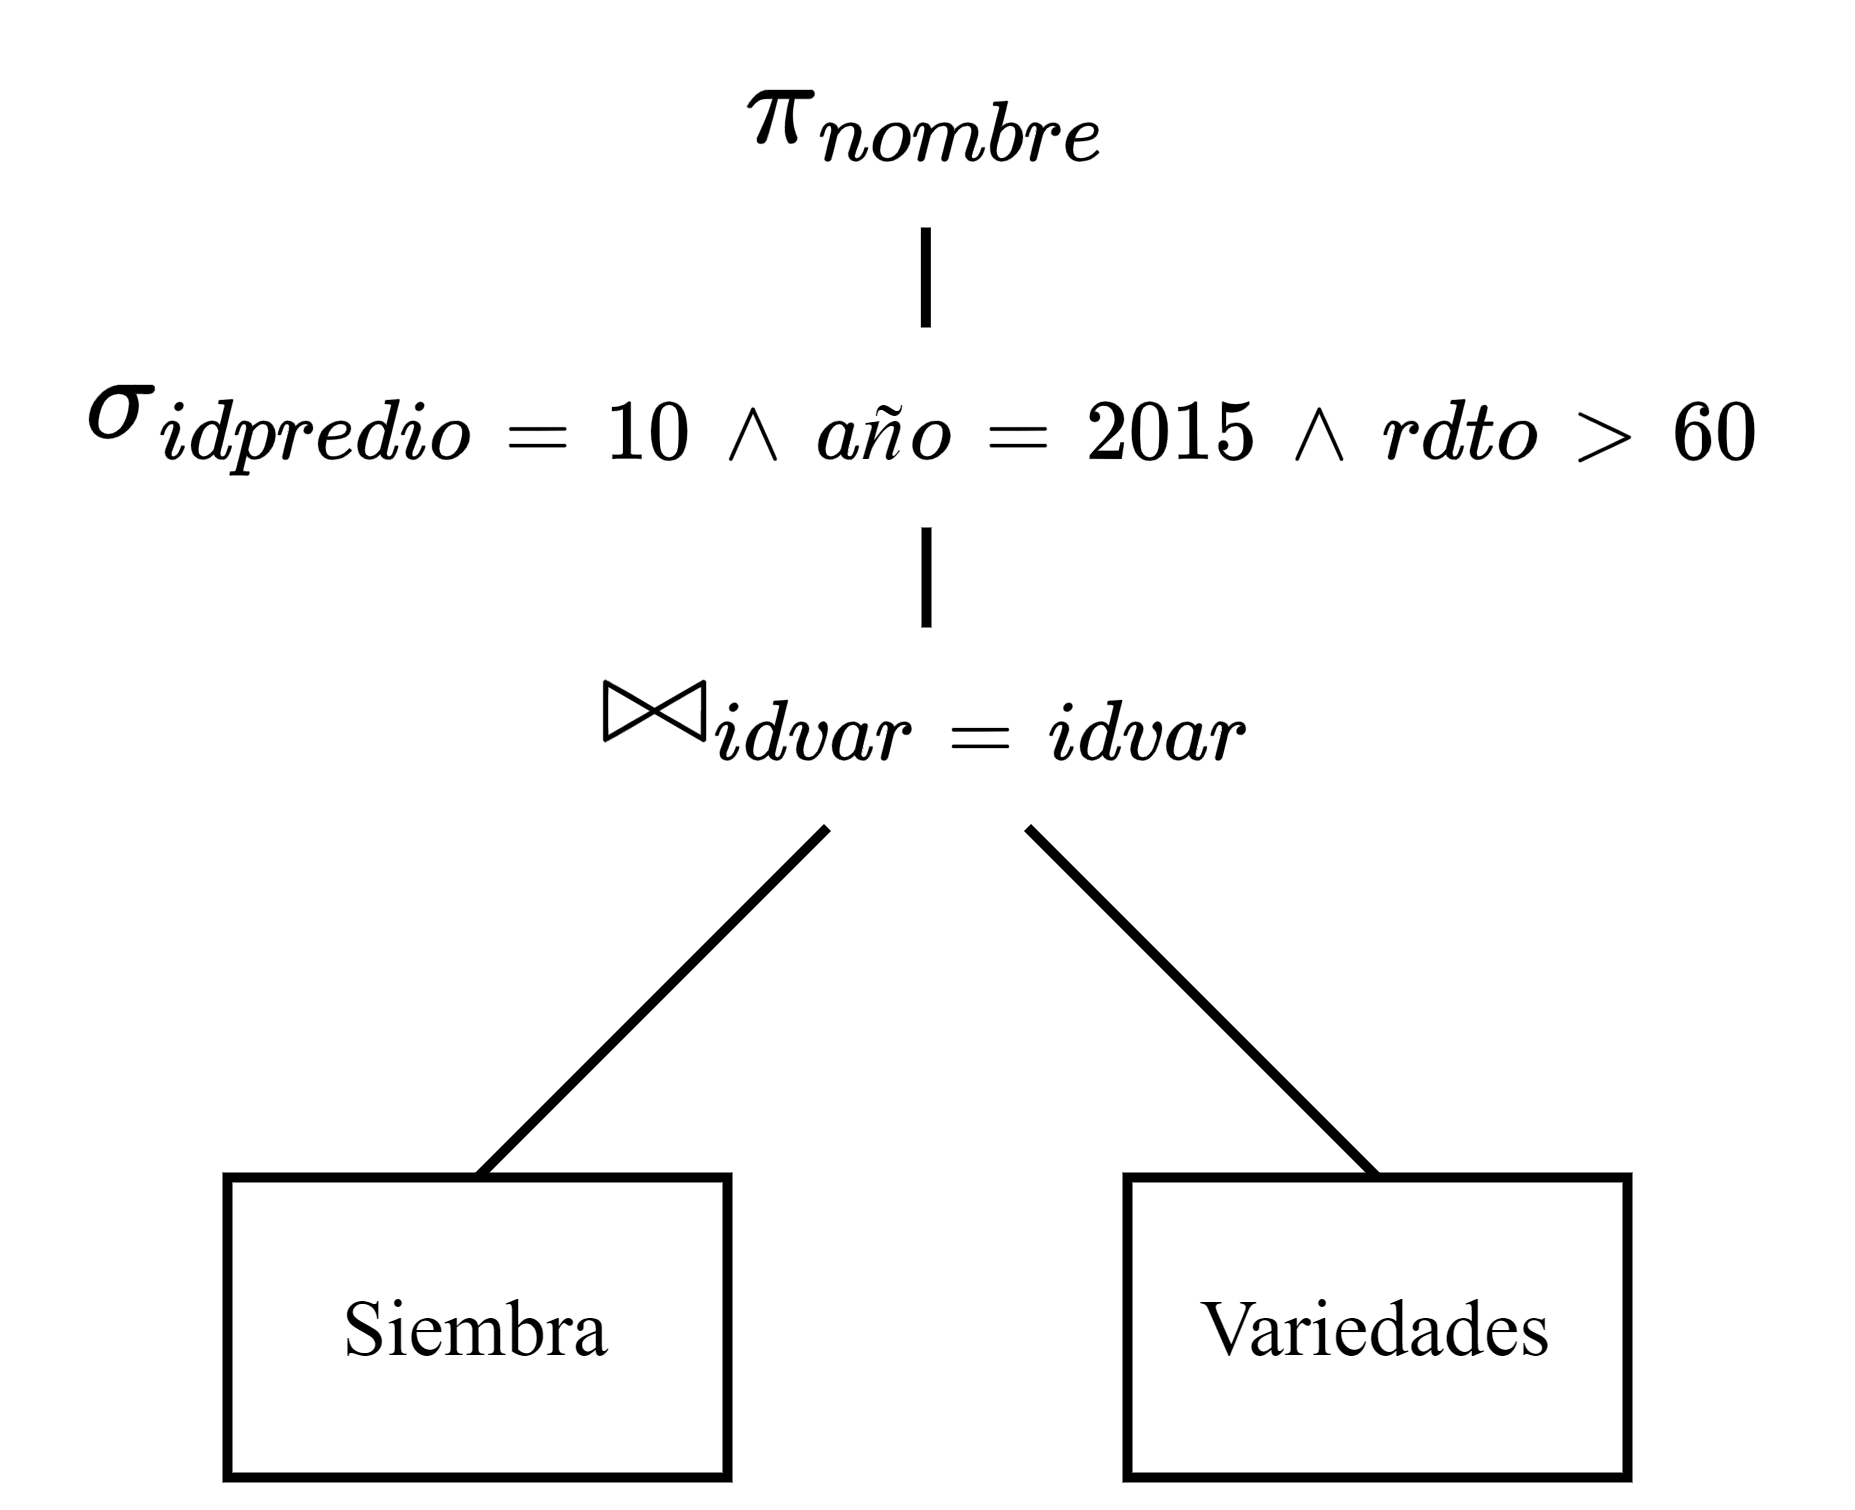
\includegraphics[width=0.5\textwidth]{img/E1-Paso-4.png}
            \end{figure}

            \item Bajar el resto de seleciones a tablas.
            \begin{figure}[H]
                \centering
                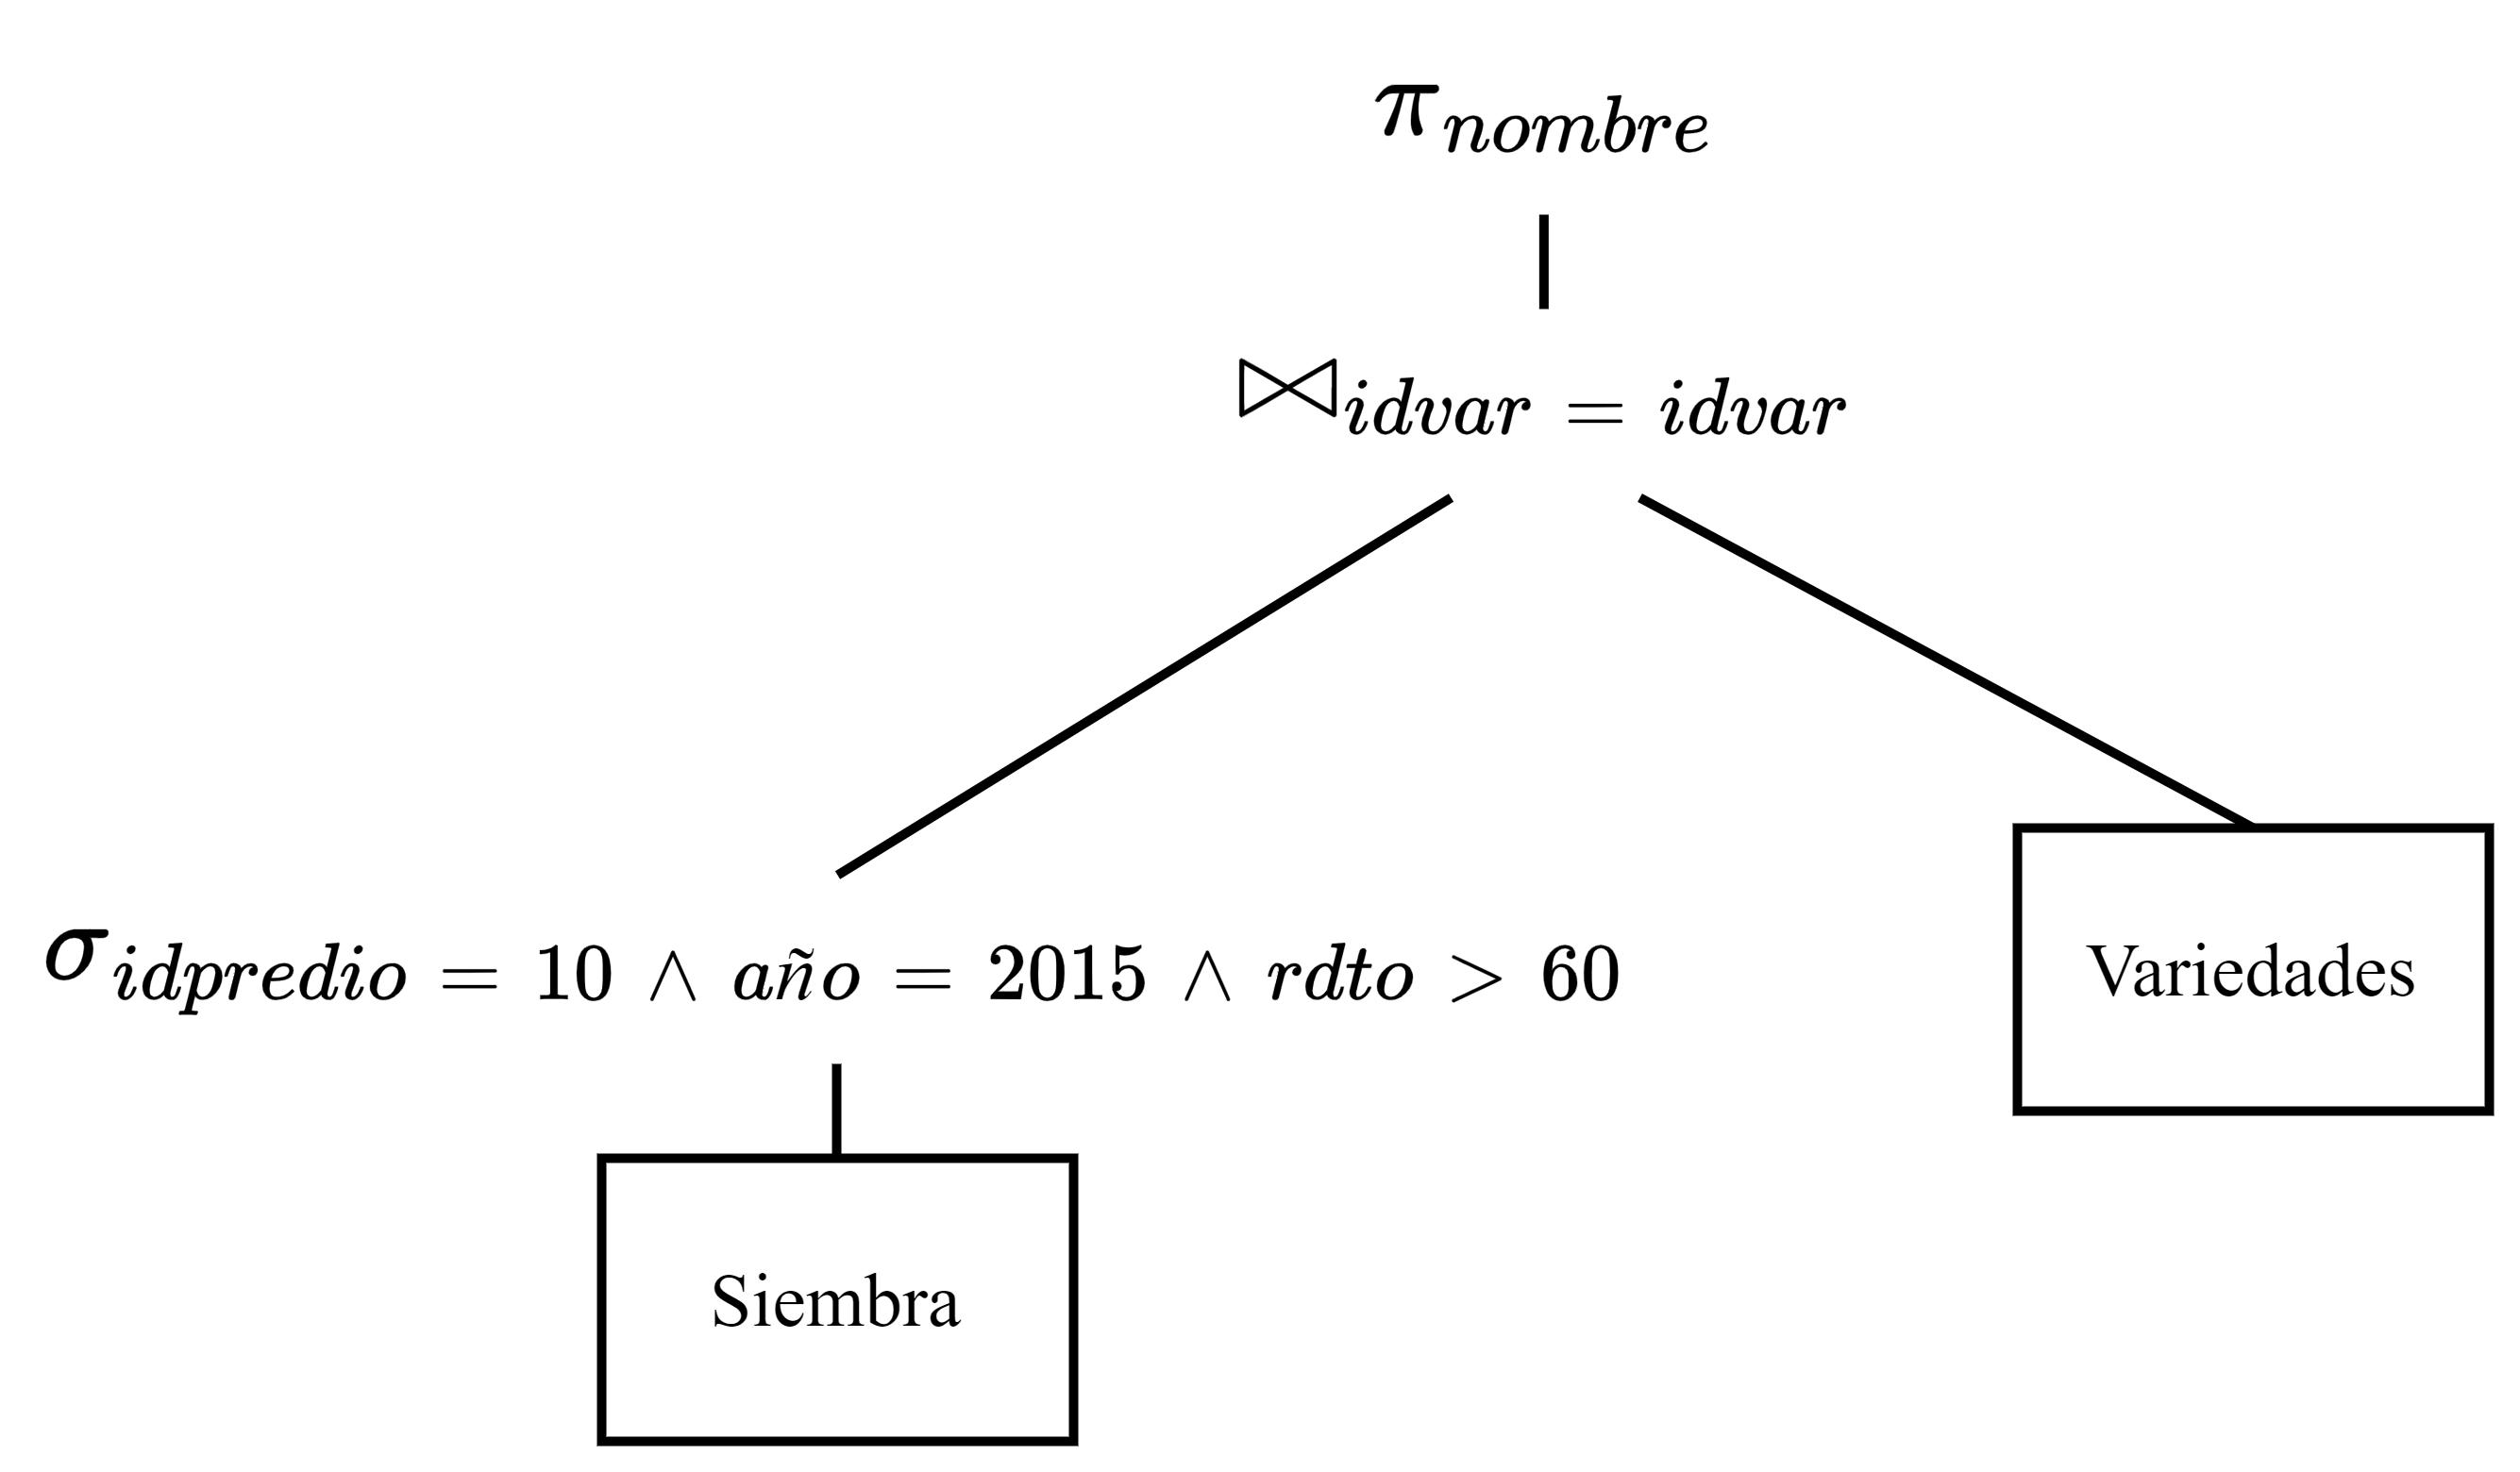
\includegraphics[width=0.6\textwidth]{img/E1-Paso-5.png}
            \end{figure}

            \newpage
            \item Proyectar los atributos necesarios.
            \begin{figure}[H]
                \centering
                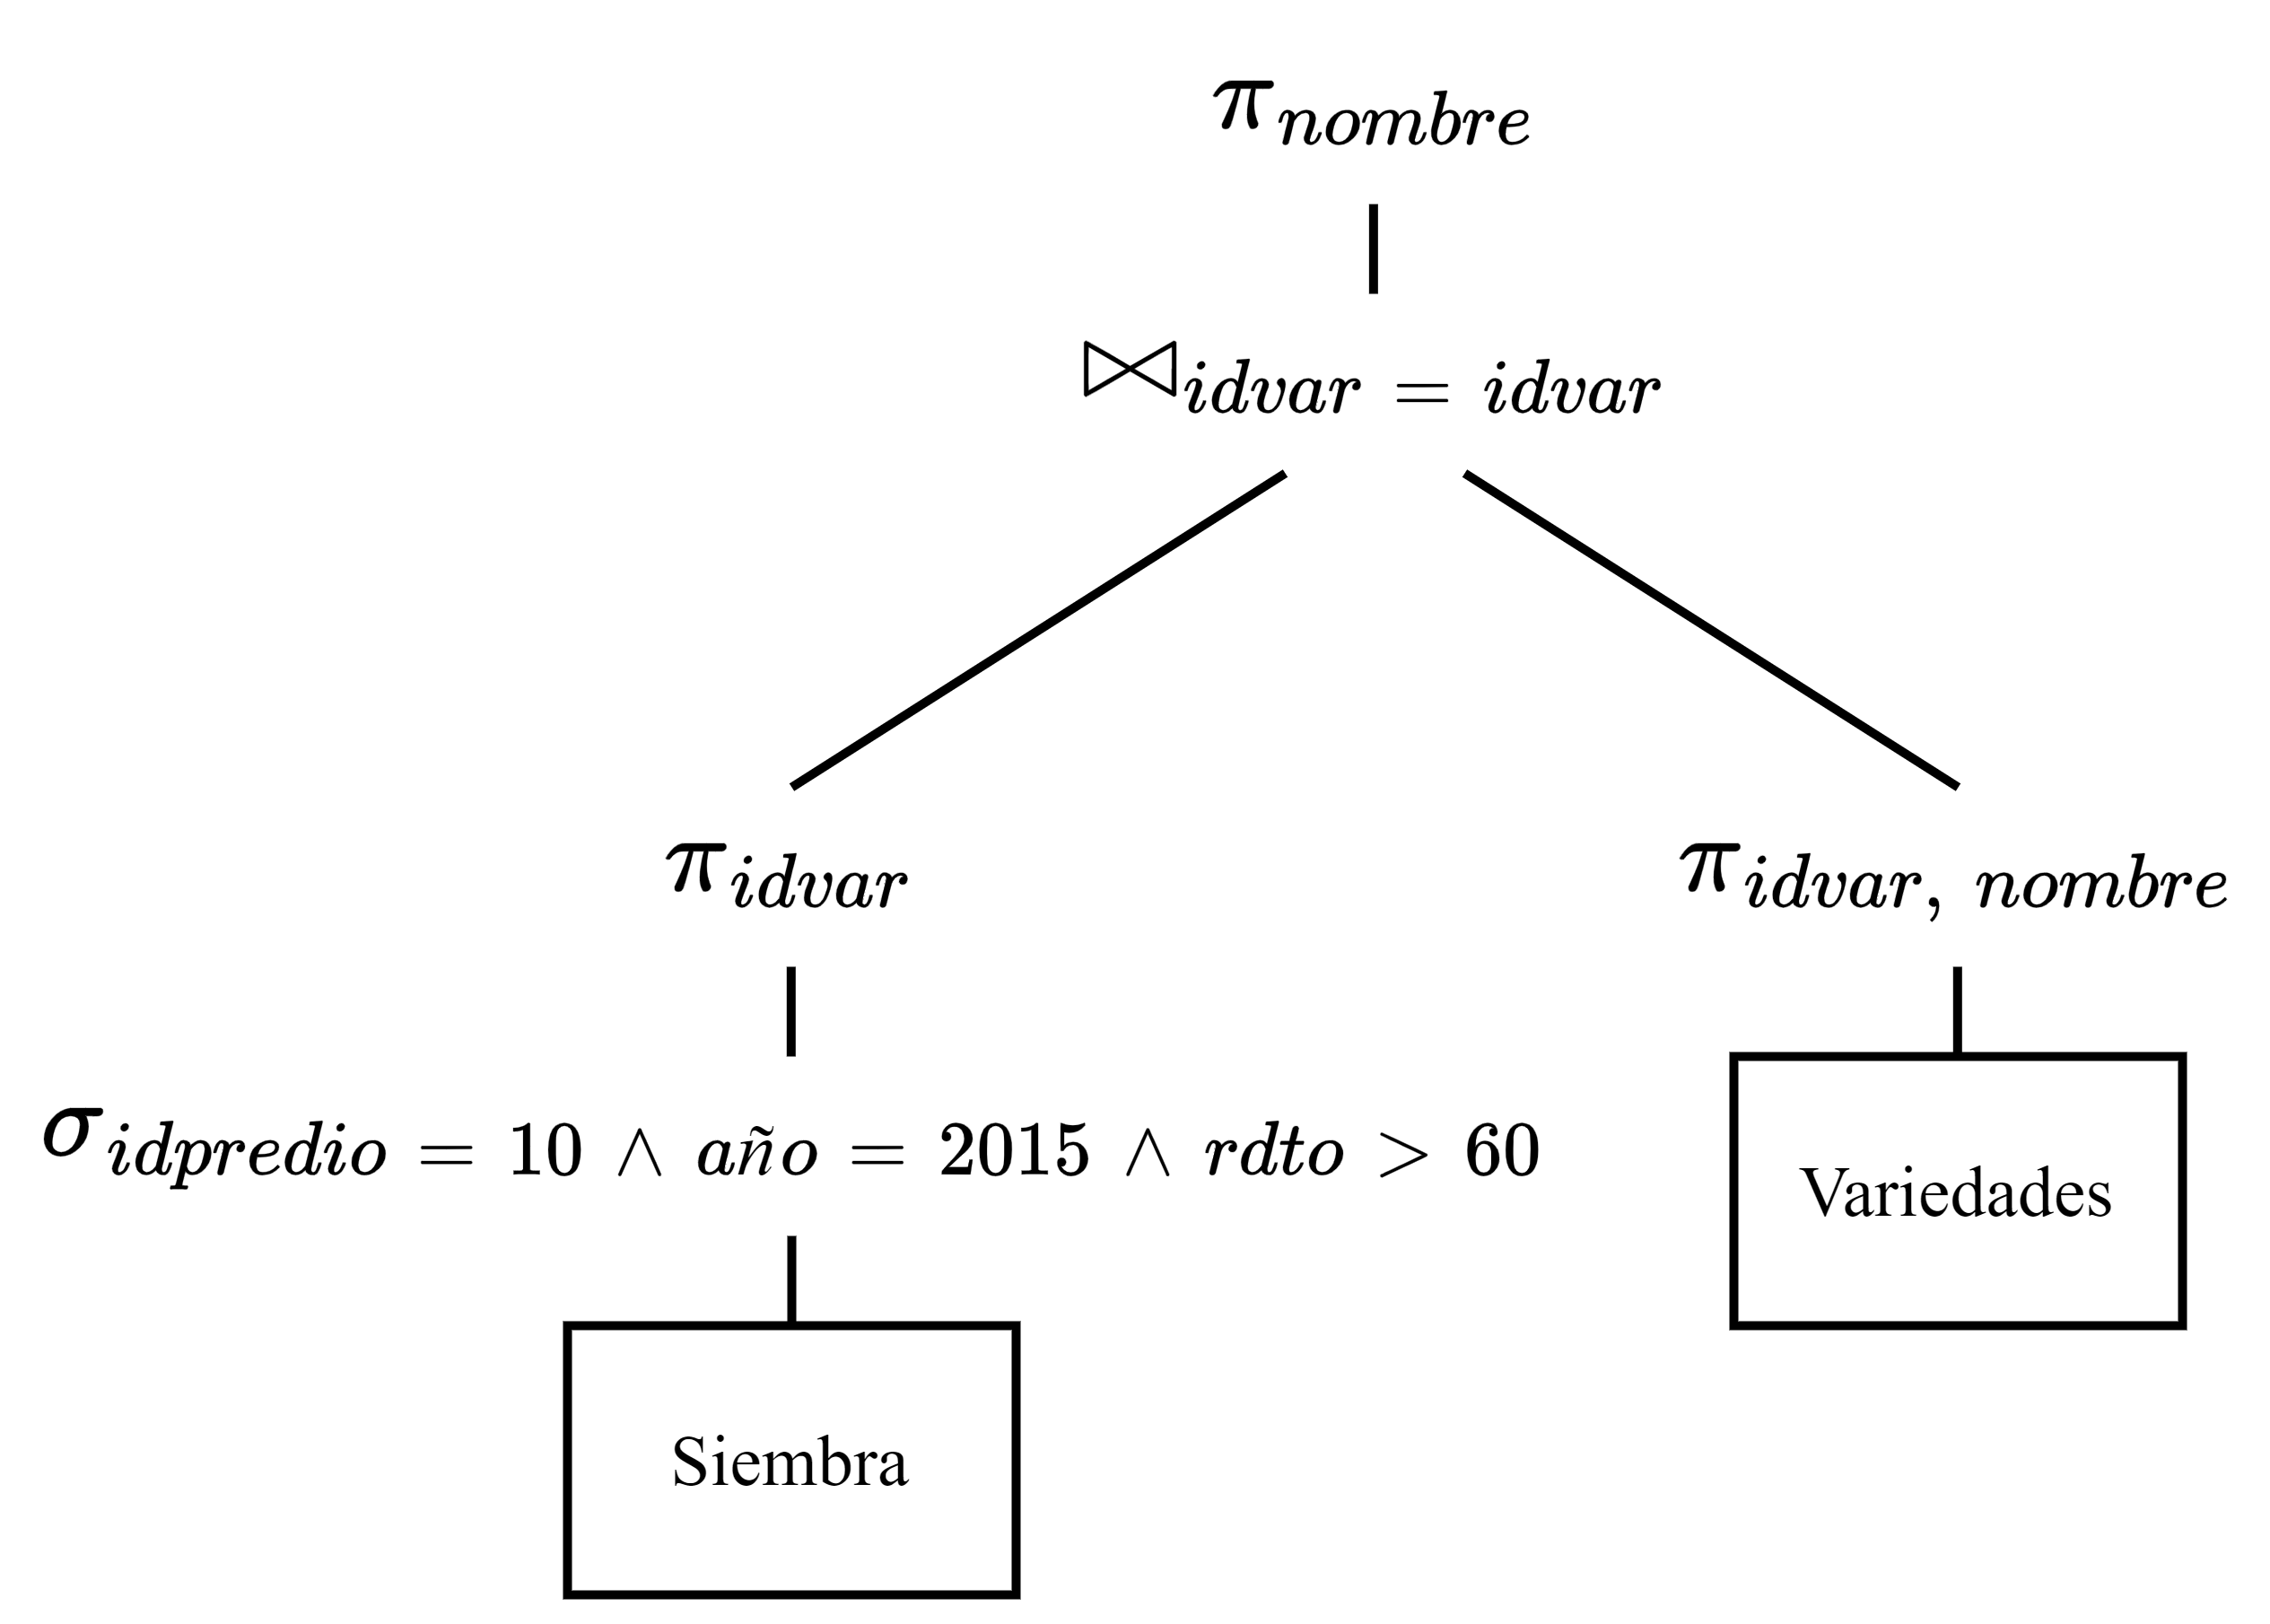
\includegraphics[width=0.65\textwidth]{img/E1-Paso-6.png}
            \end{figure}
        \end{enumerate}
    \end{itemize}

    \item Listar los nombres de los predios que tienen una \hlcolor{Salmon!40}{superficie mayor a $4500m^2$, de la comuna de 'tortel' y que han tenido la variedad 'hibrido'(nombre variedad) durante a\~no 2020}.
    \begin{itemize}
        \item SQL.
        \begin{verbatim}
SELECT P.nombrepredio
FROM Predios P,
     Siembra S,
     Variedades V,
WHERE P.idpredio = S.idpredio 
AND S.idvar = V.idvar 
AND P.superficie > 4500
AND P.comuna = 'tortel'
AND V.nombre = 'hibrido'
AND S.año = 2020;
        \end{verbatim}

        \item Algebra Relacional.
        \begin{align*}
            \scalebox{1.5}{$\pi$}_{\text{nombrepredio}} (
                \scalebox{1.5}{$\sigma$}_{
                    \scalebox{0.8}{
                        $\begin{array}{l}
                            \text{idpredio} = \text{idpredio} \; \wedge \\
                            \text{idvar} = \text{idvar} \; \wedge \\
                            \text{superficie} > 4500 \; \wedge \\
                            \text{comuna} = \text{'tortel'} \; \wedge \\
                            \text{nombre} = \text{'hibrido'} \; \wedge \\
                            \text{a\~no} = 2015
                        \end{array}$
                    }
                } (
                    \text{Predios}_{\scalebox{1.3}{$\Join$}} (
                        \text{Siembra}_{\scalebox{1.3}{$\Join$}} \text{Variedad}
                    )
                )
            )
        \end{align*}
        
        \newpage
        \item Arbol Canonico.
        \begin{figure}[H]
            \centering
            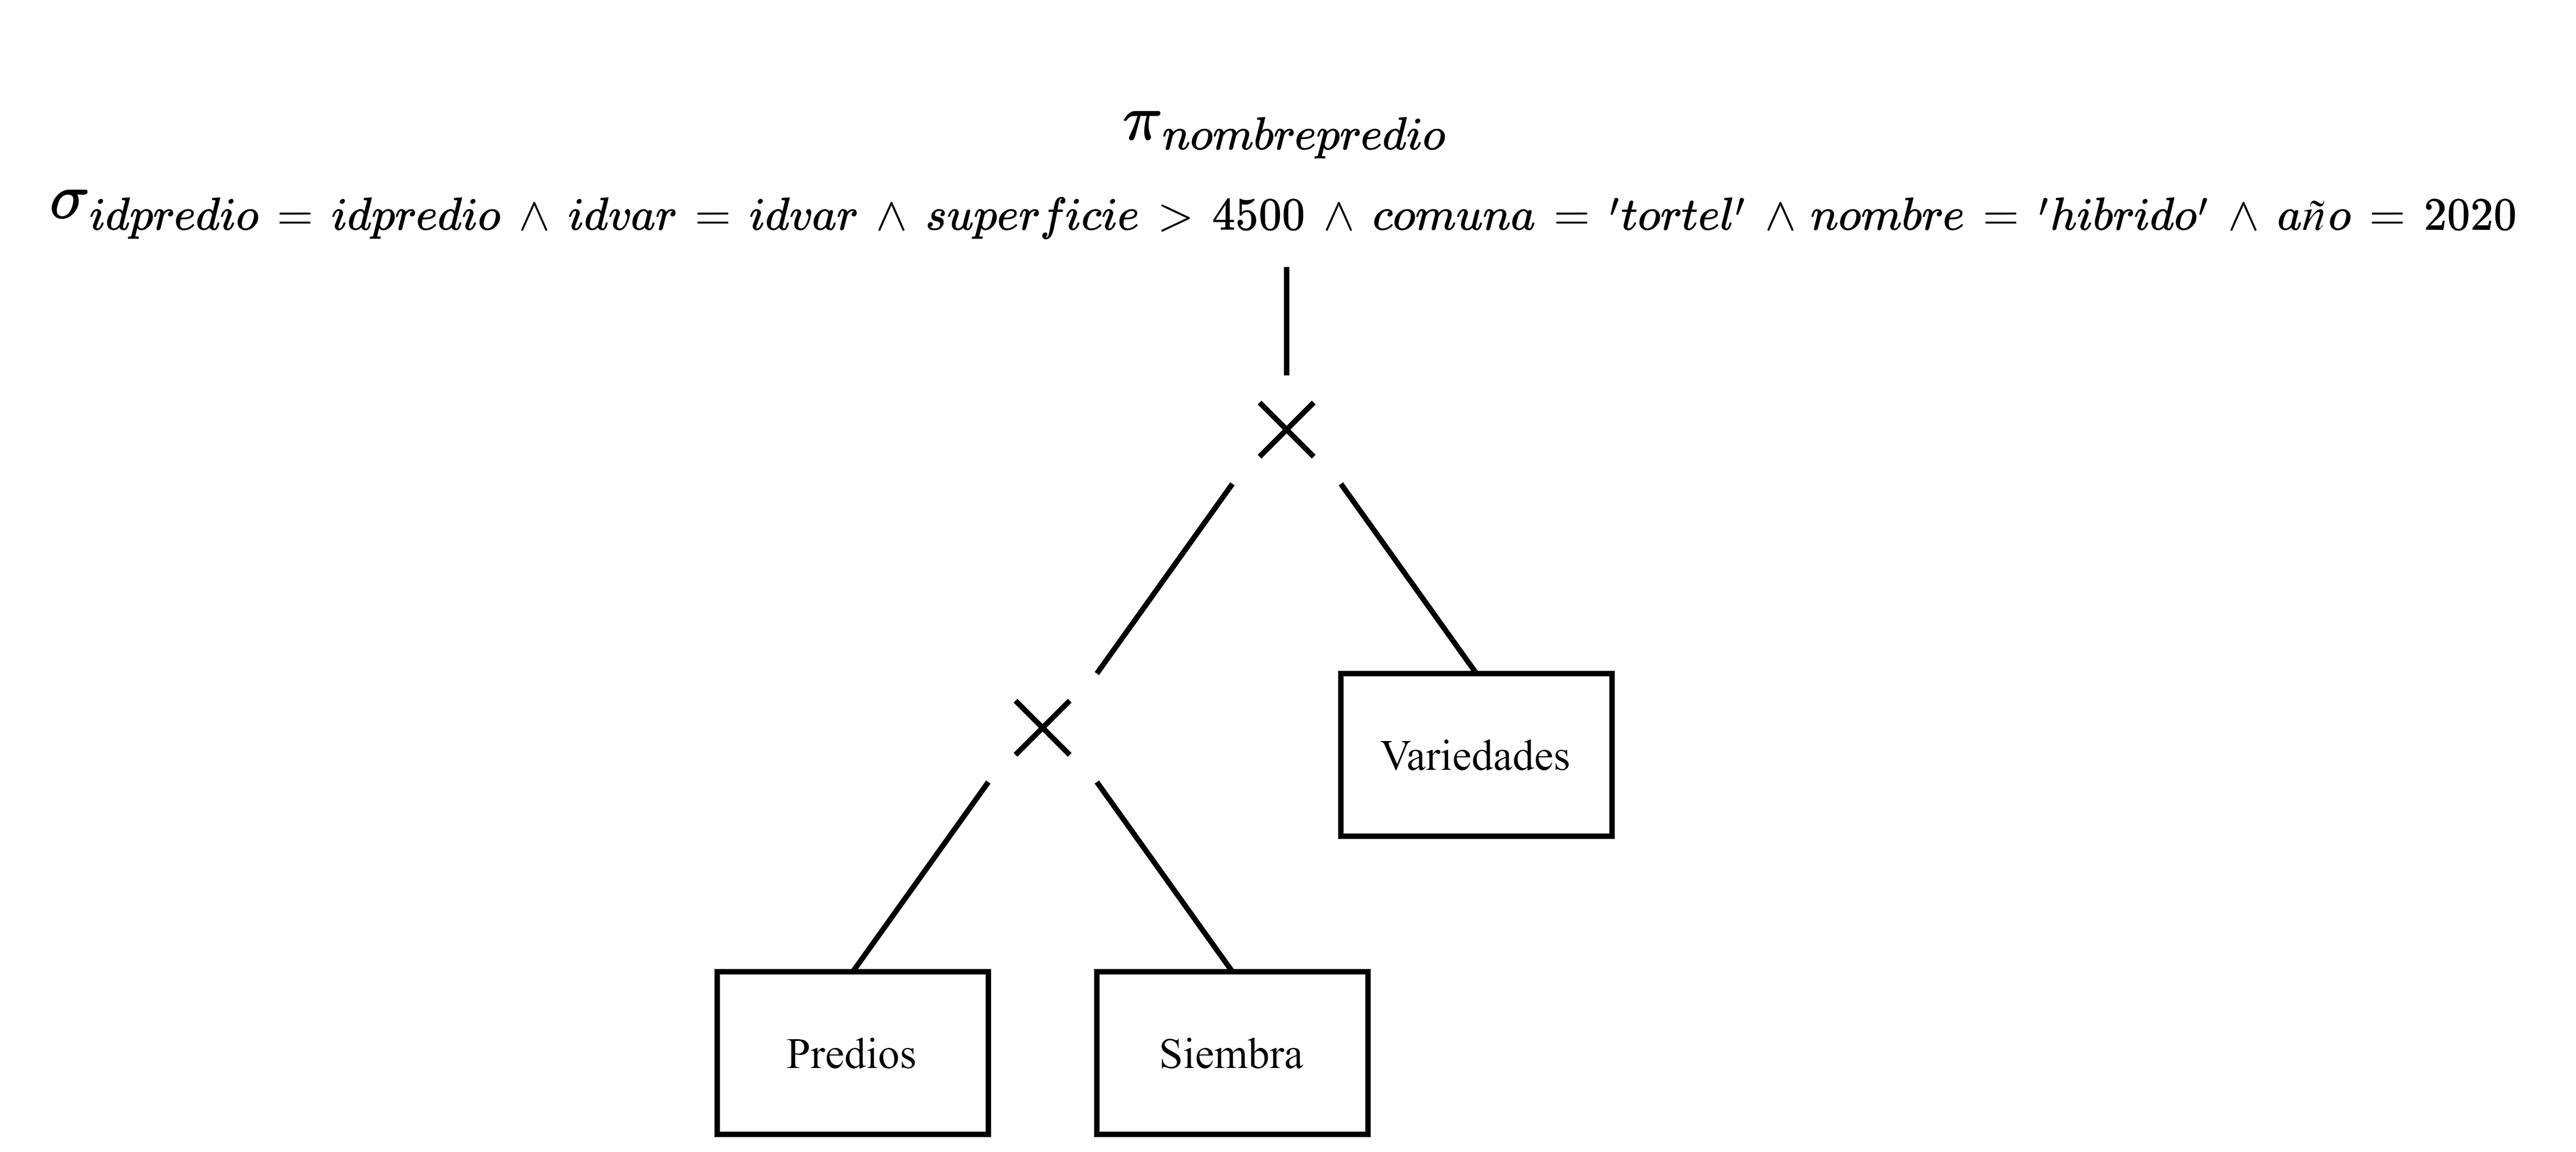
\includegraphics[width=\textwidth]{img/E2-Canonico.png}
        \end{figure}

        \item Optimizaci\'on.
        \begin{enumerate}
            \item Separar las selecciones.
            \begin{figure}[H]
                \centering
                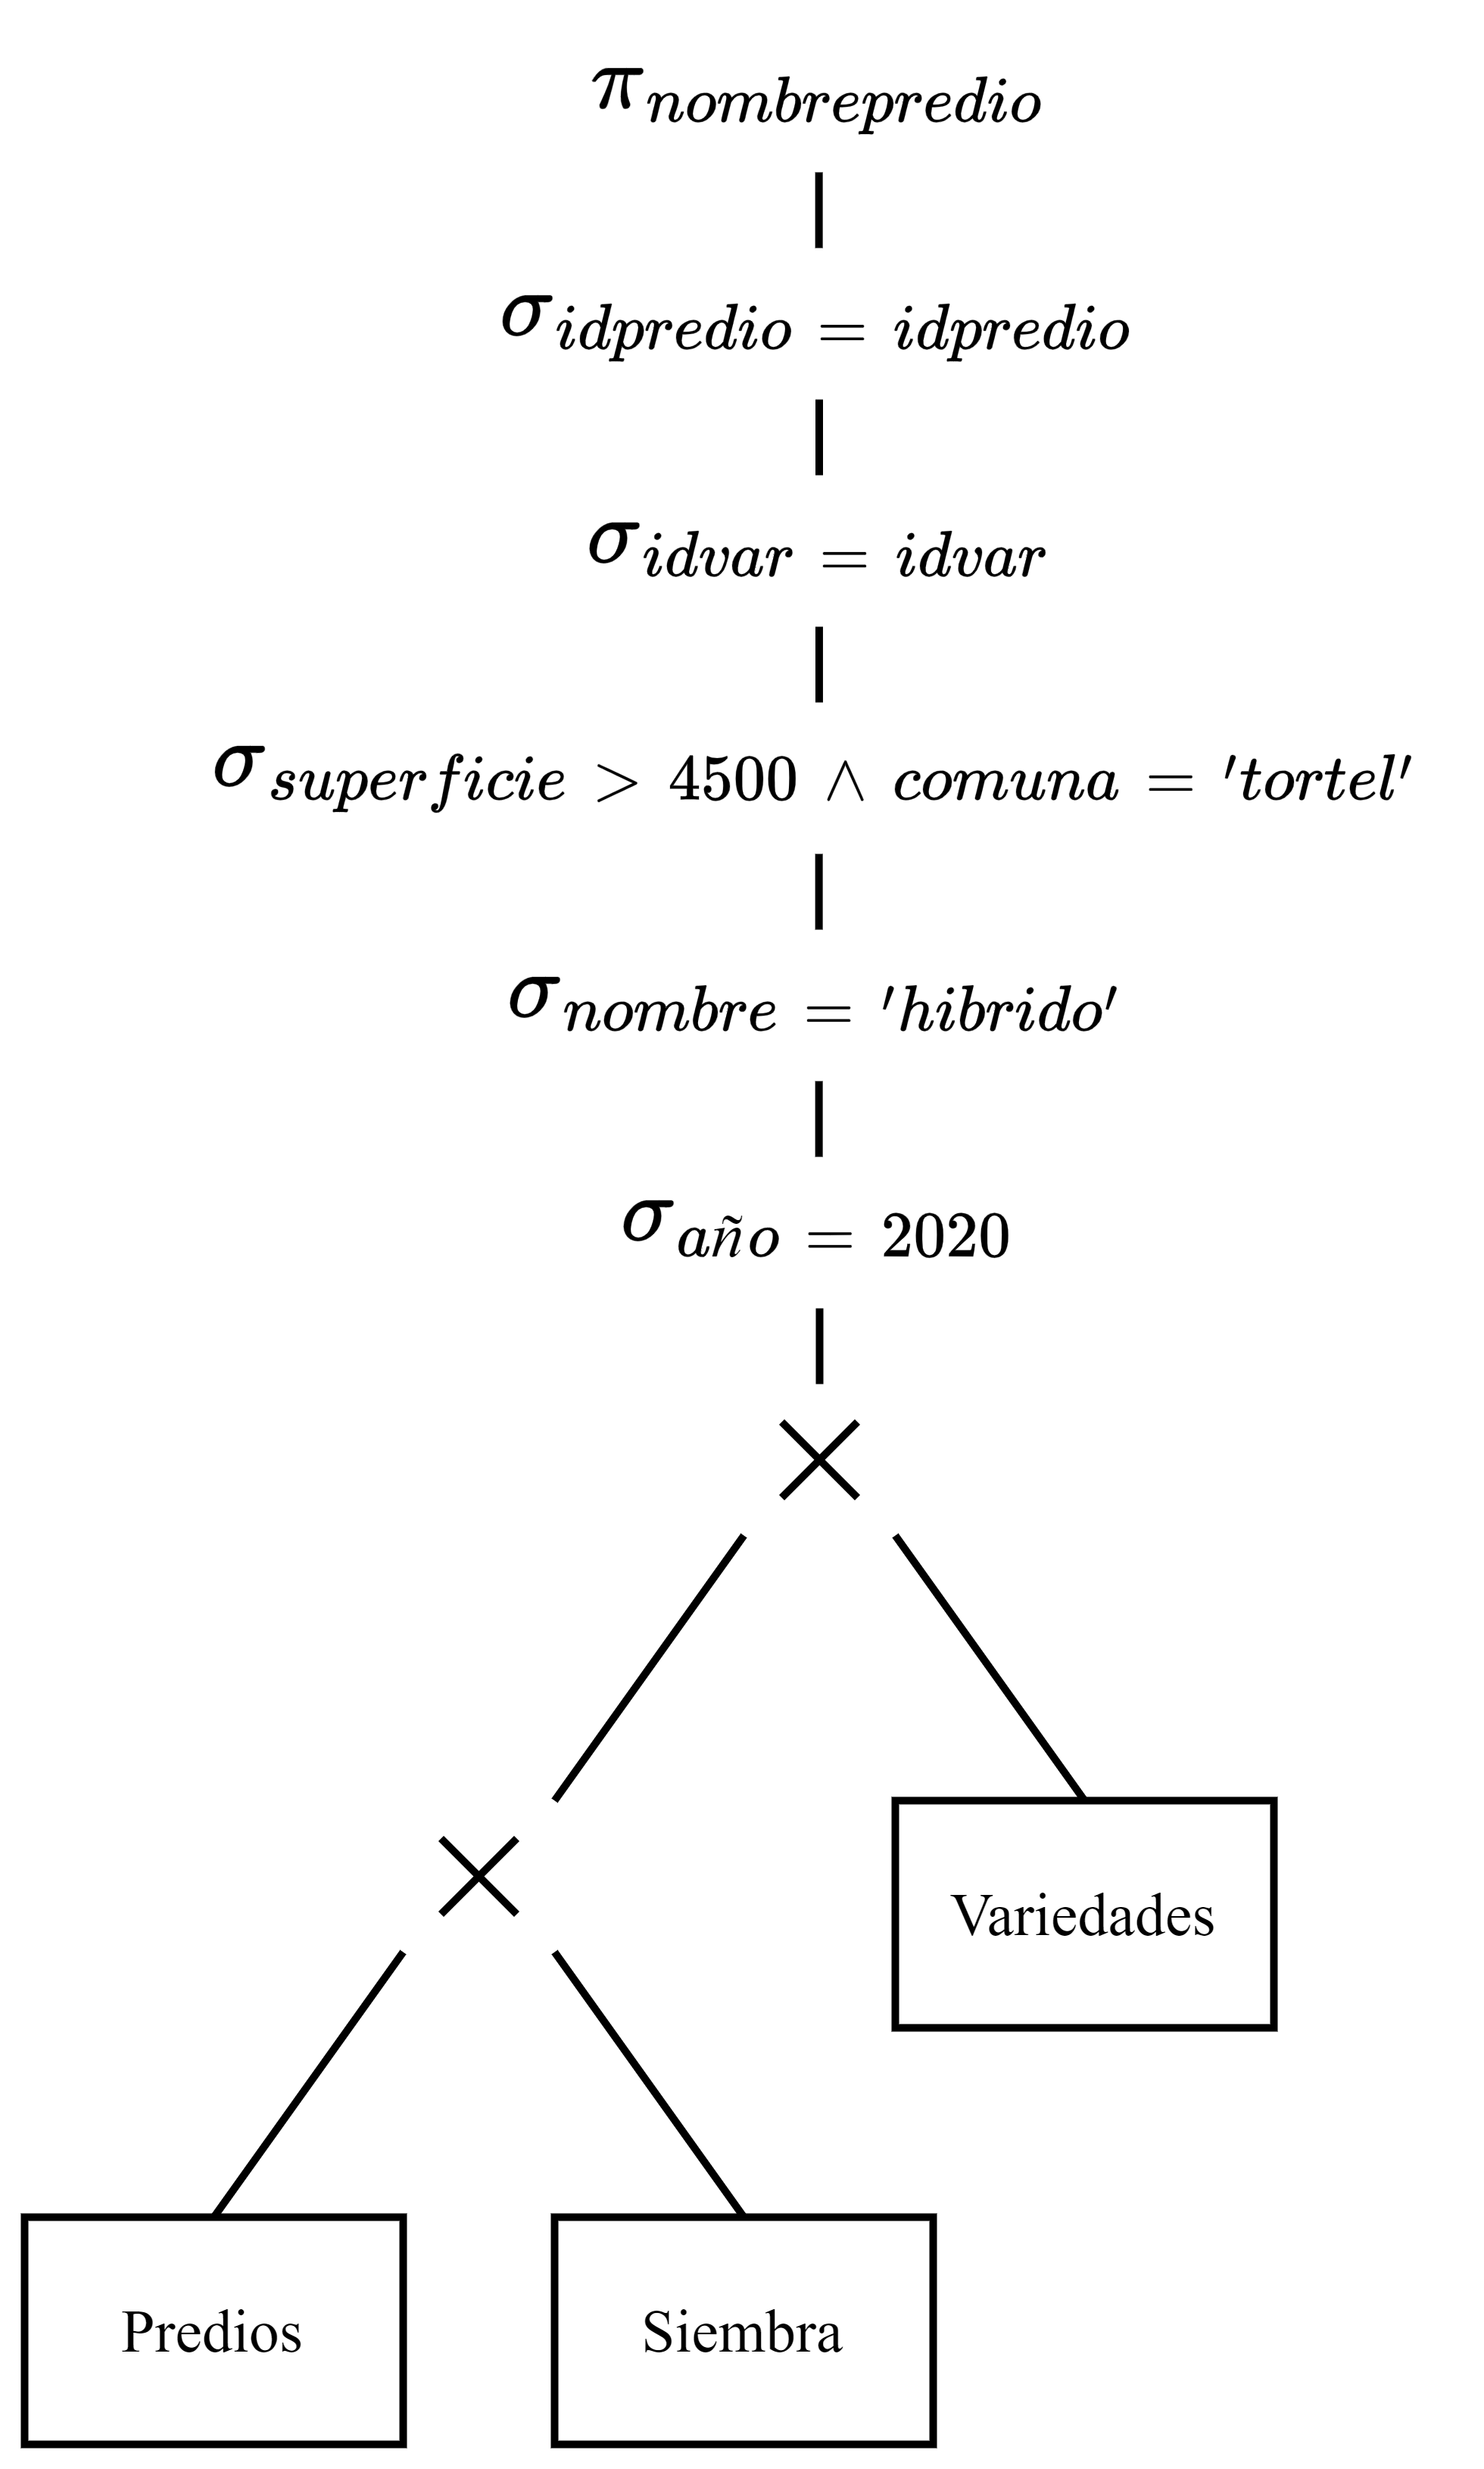
\includegraphics[width=0.5\textwidth]{img/E2-Paso-1.png}
            \end{figure}

            \newpage
            \item Permutar tablas si es necesario.
            \begin{figure}[H]
                \centering
                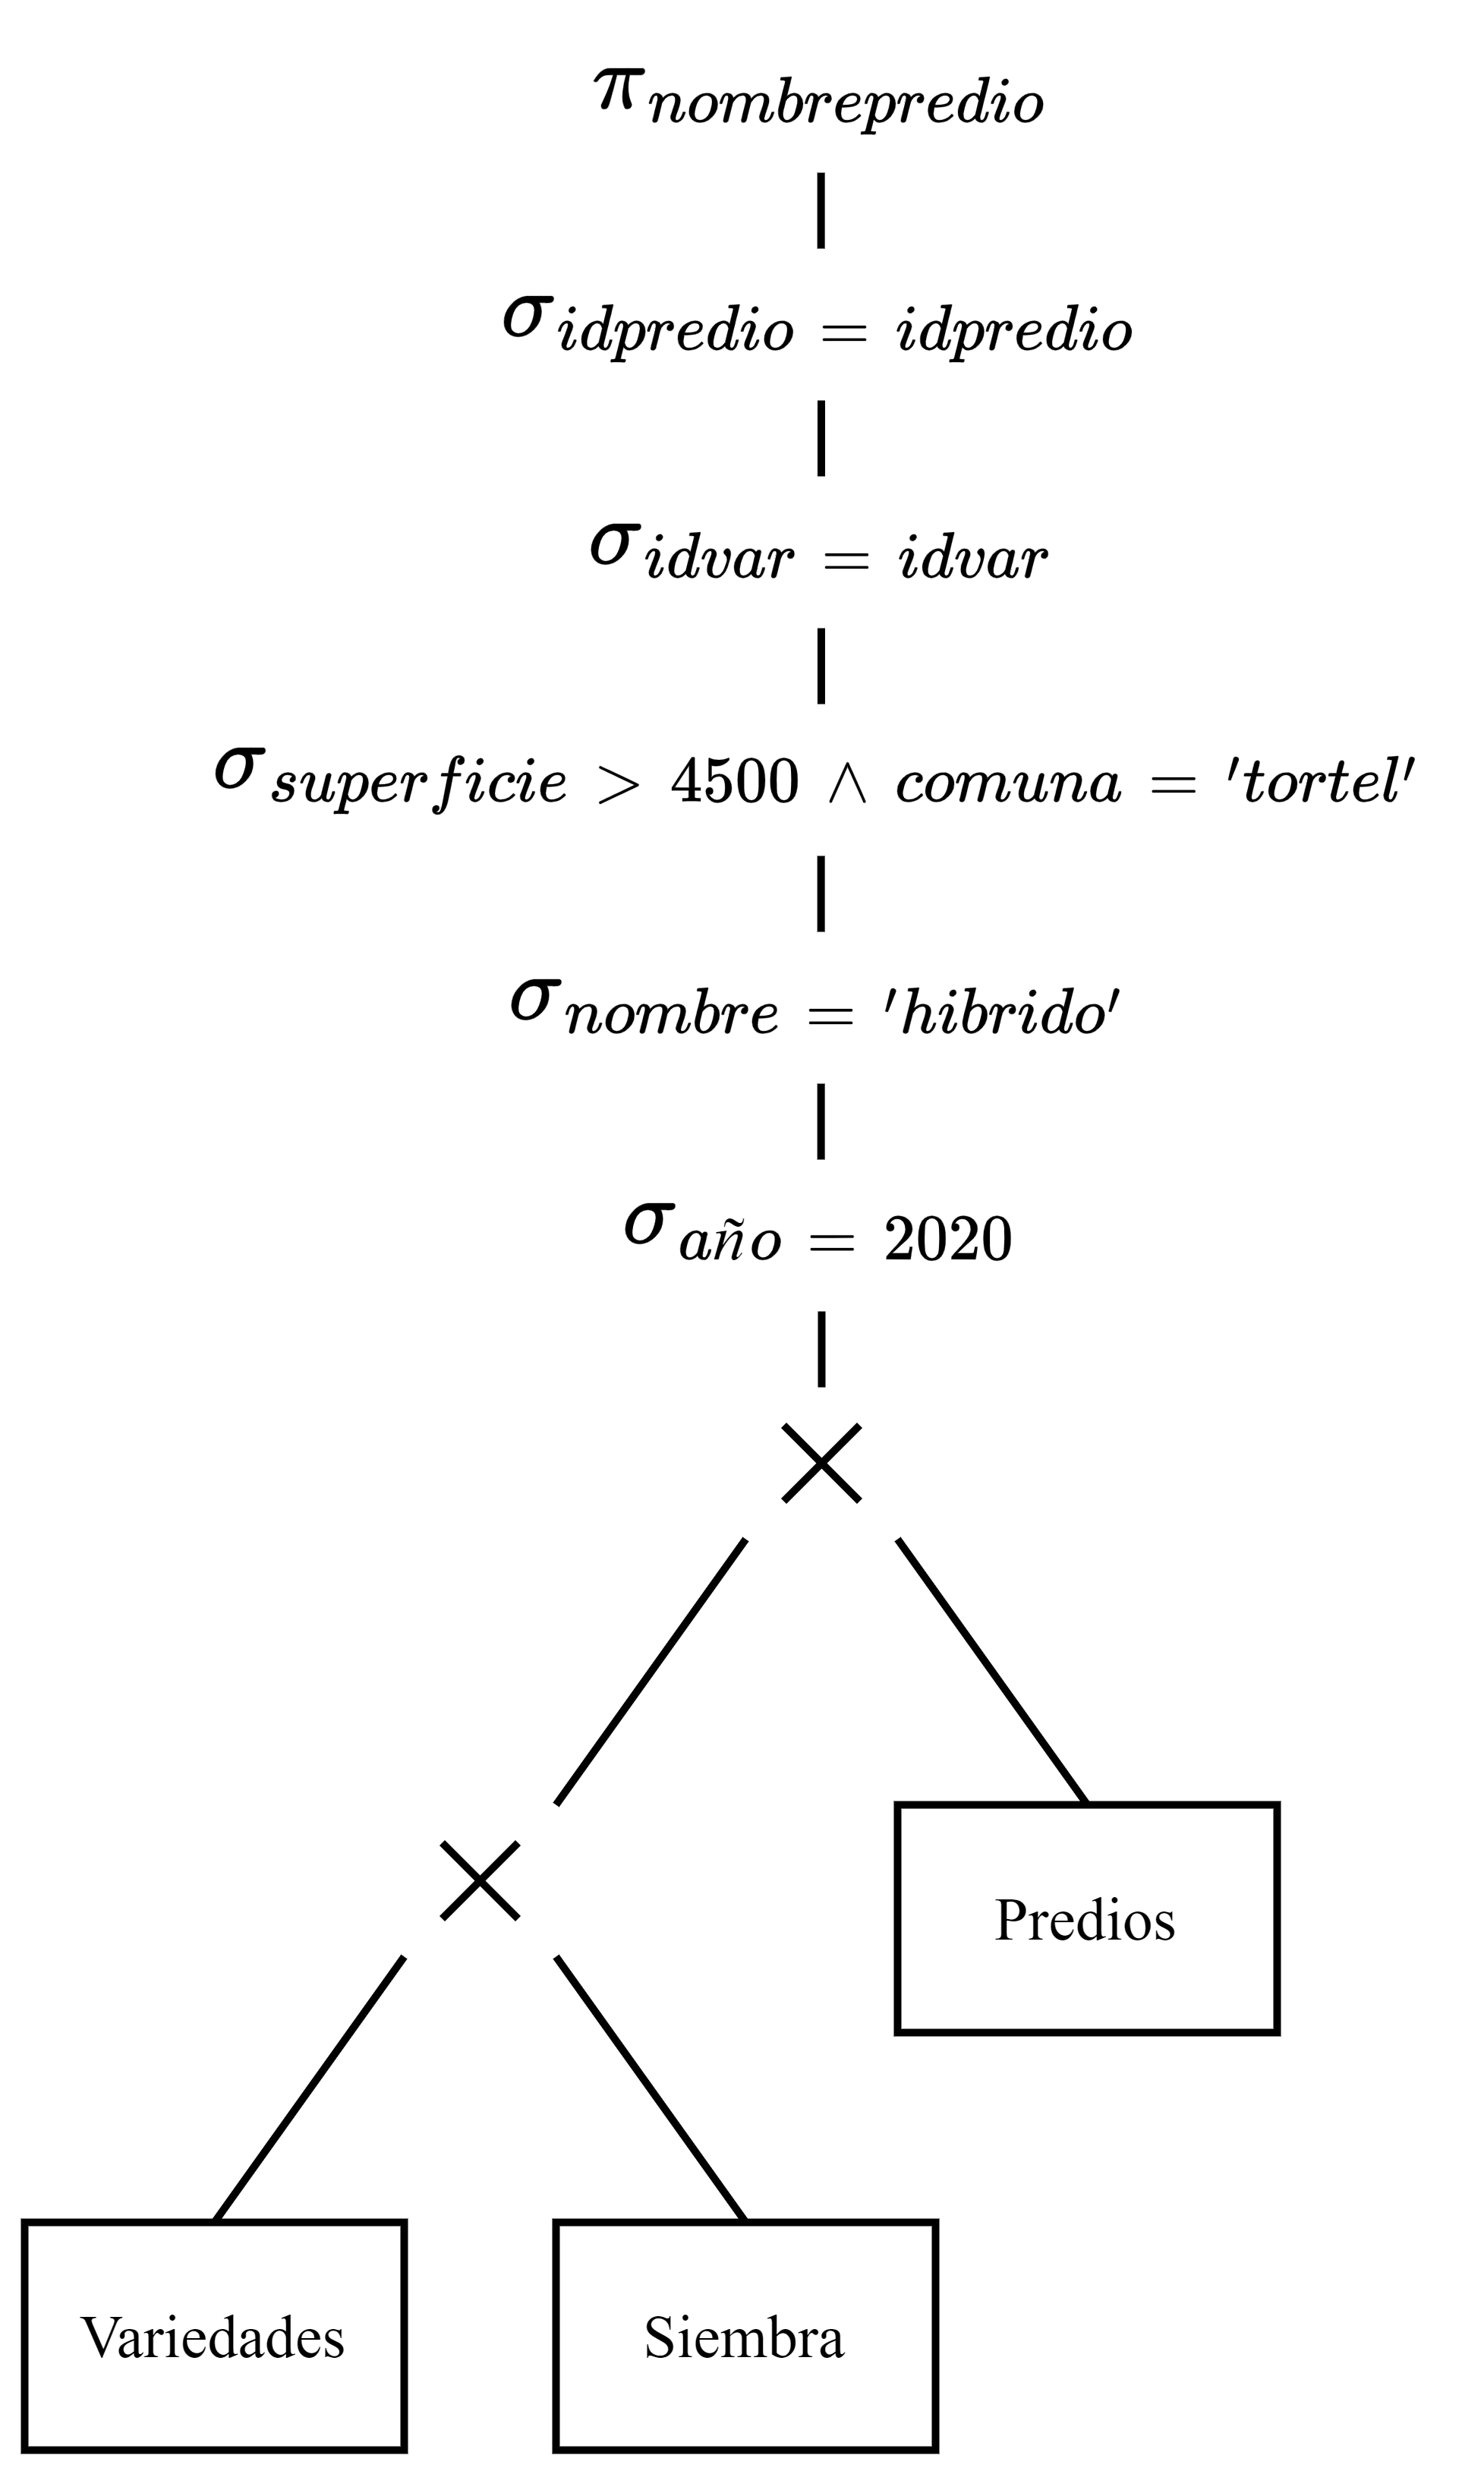
\includegraphics[width=0.4\textwidth]{img/E2-Paso-2.png}
            \end{figure}

            \item Bajar las seleciones que son $\times$ para $\Join$.
            \begin{figure}[H]
                \centering
                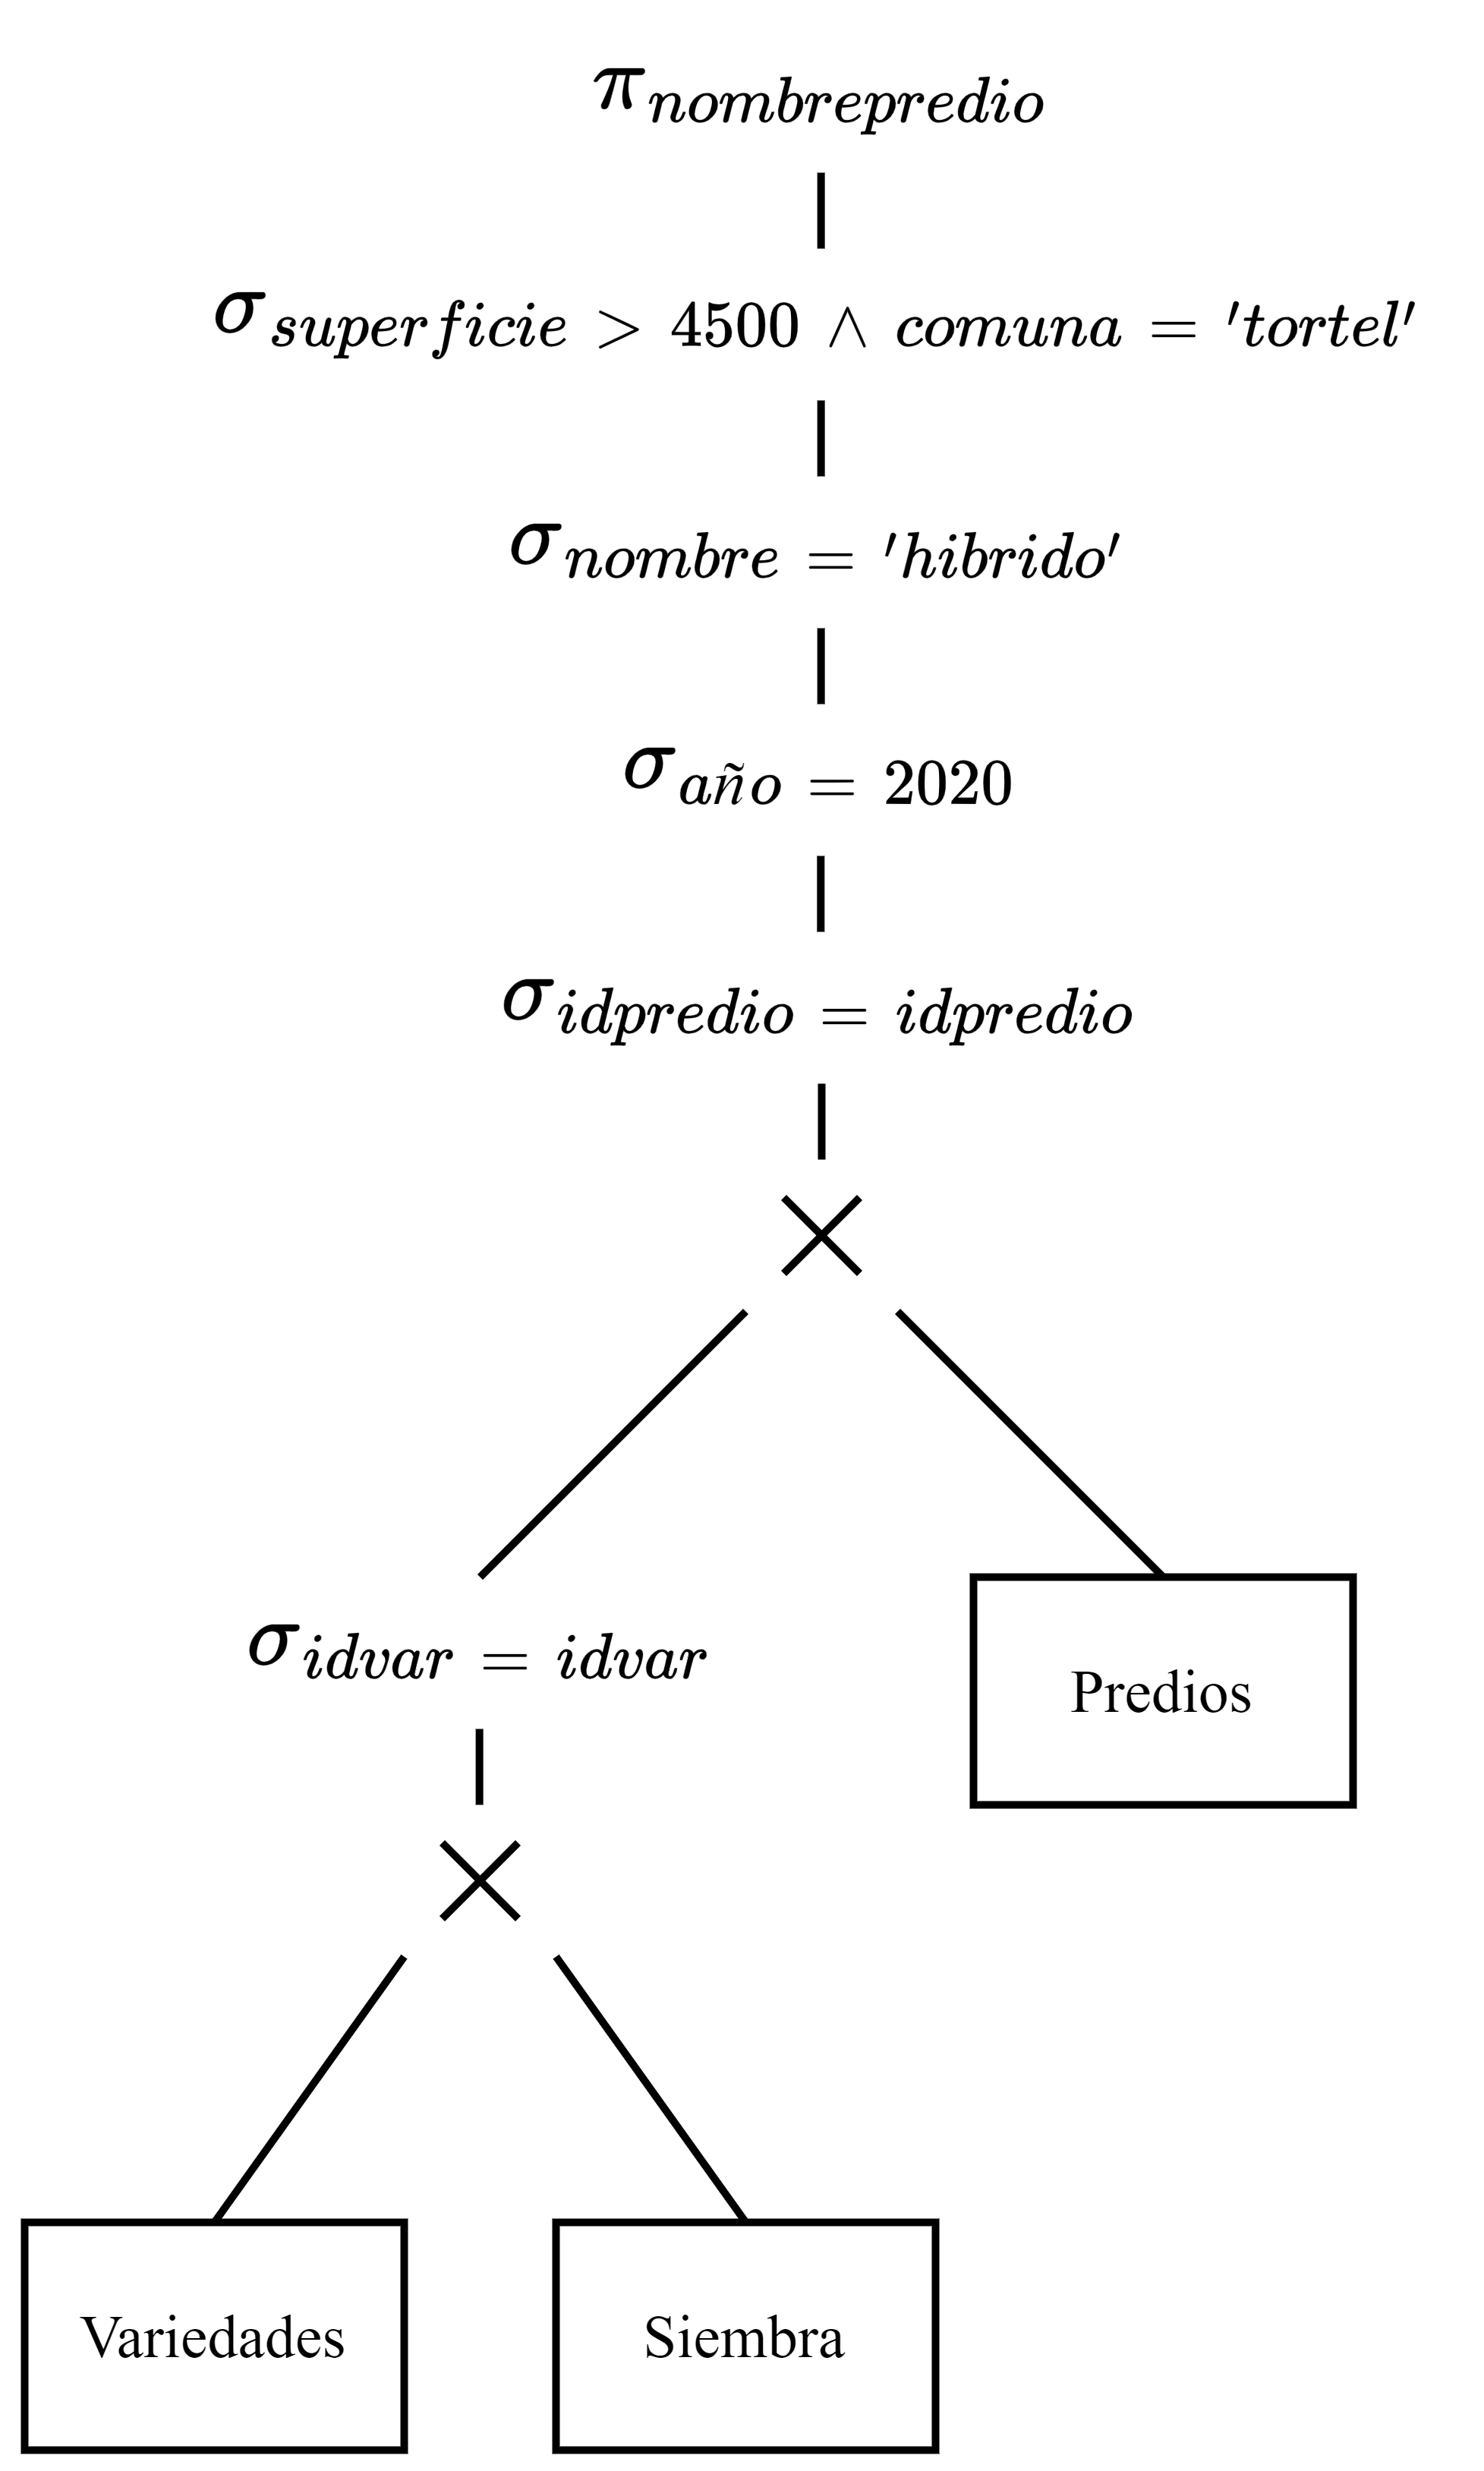
\includegraphics[width=0.4\textwidth]{img/E2-Paso-3.png}
            \end{figure}

            \newpage
            \item Cambio $\times$ por $\Join$.
            \begin{figure}[H]
                \centering
                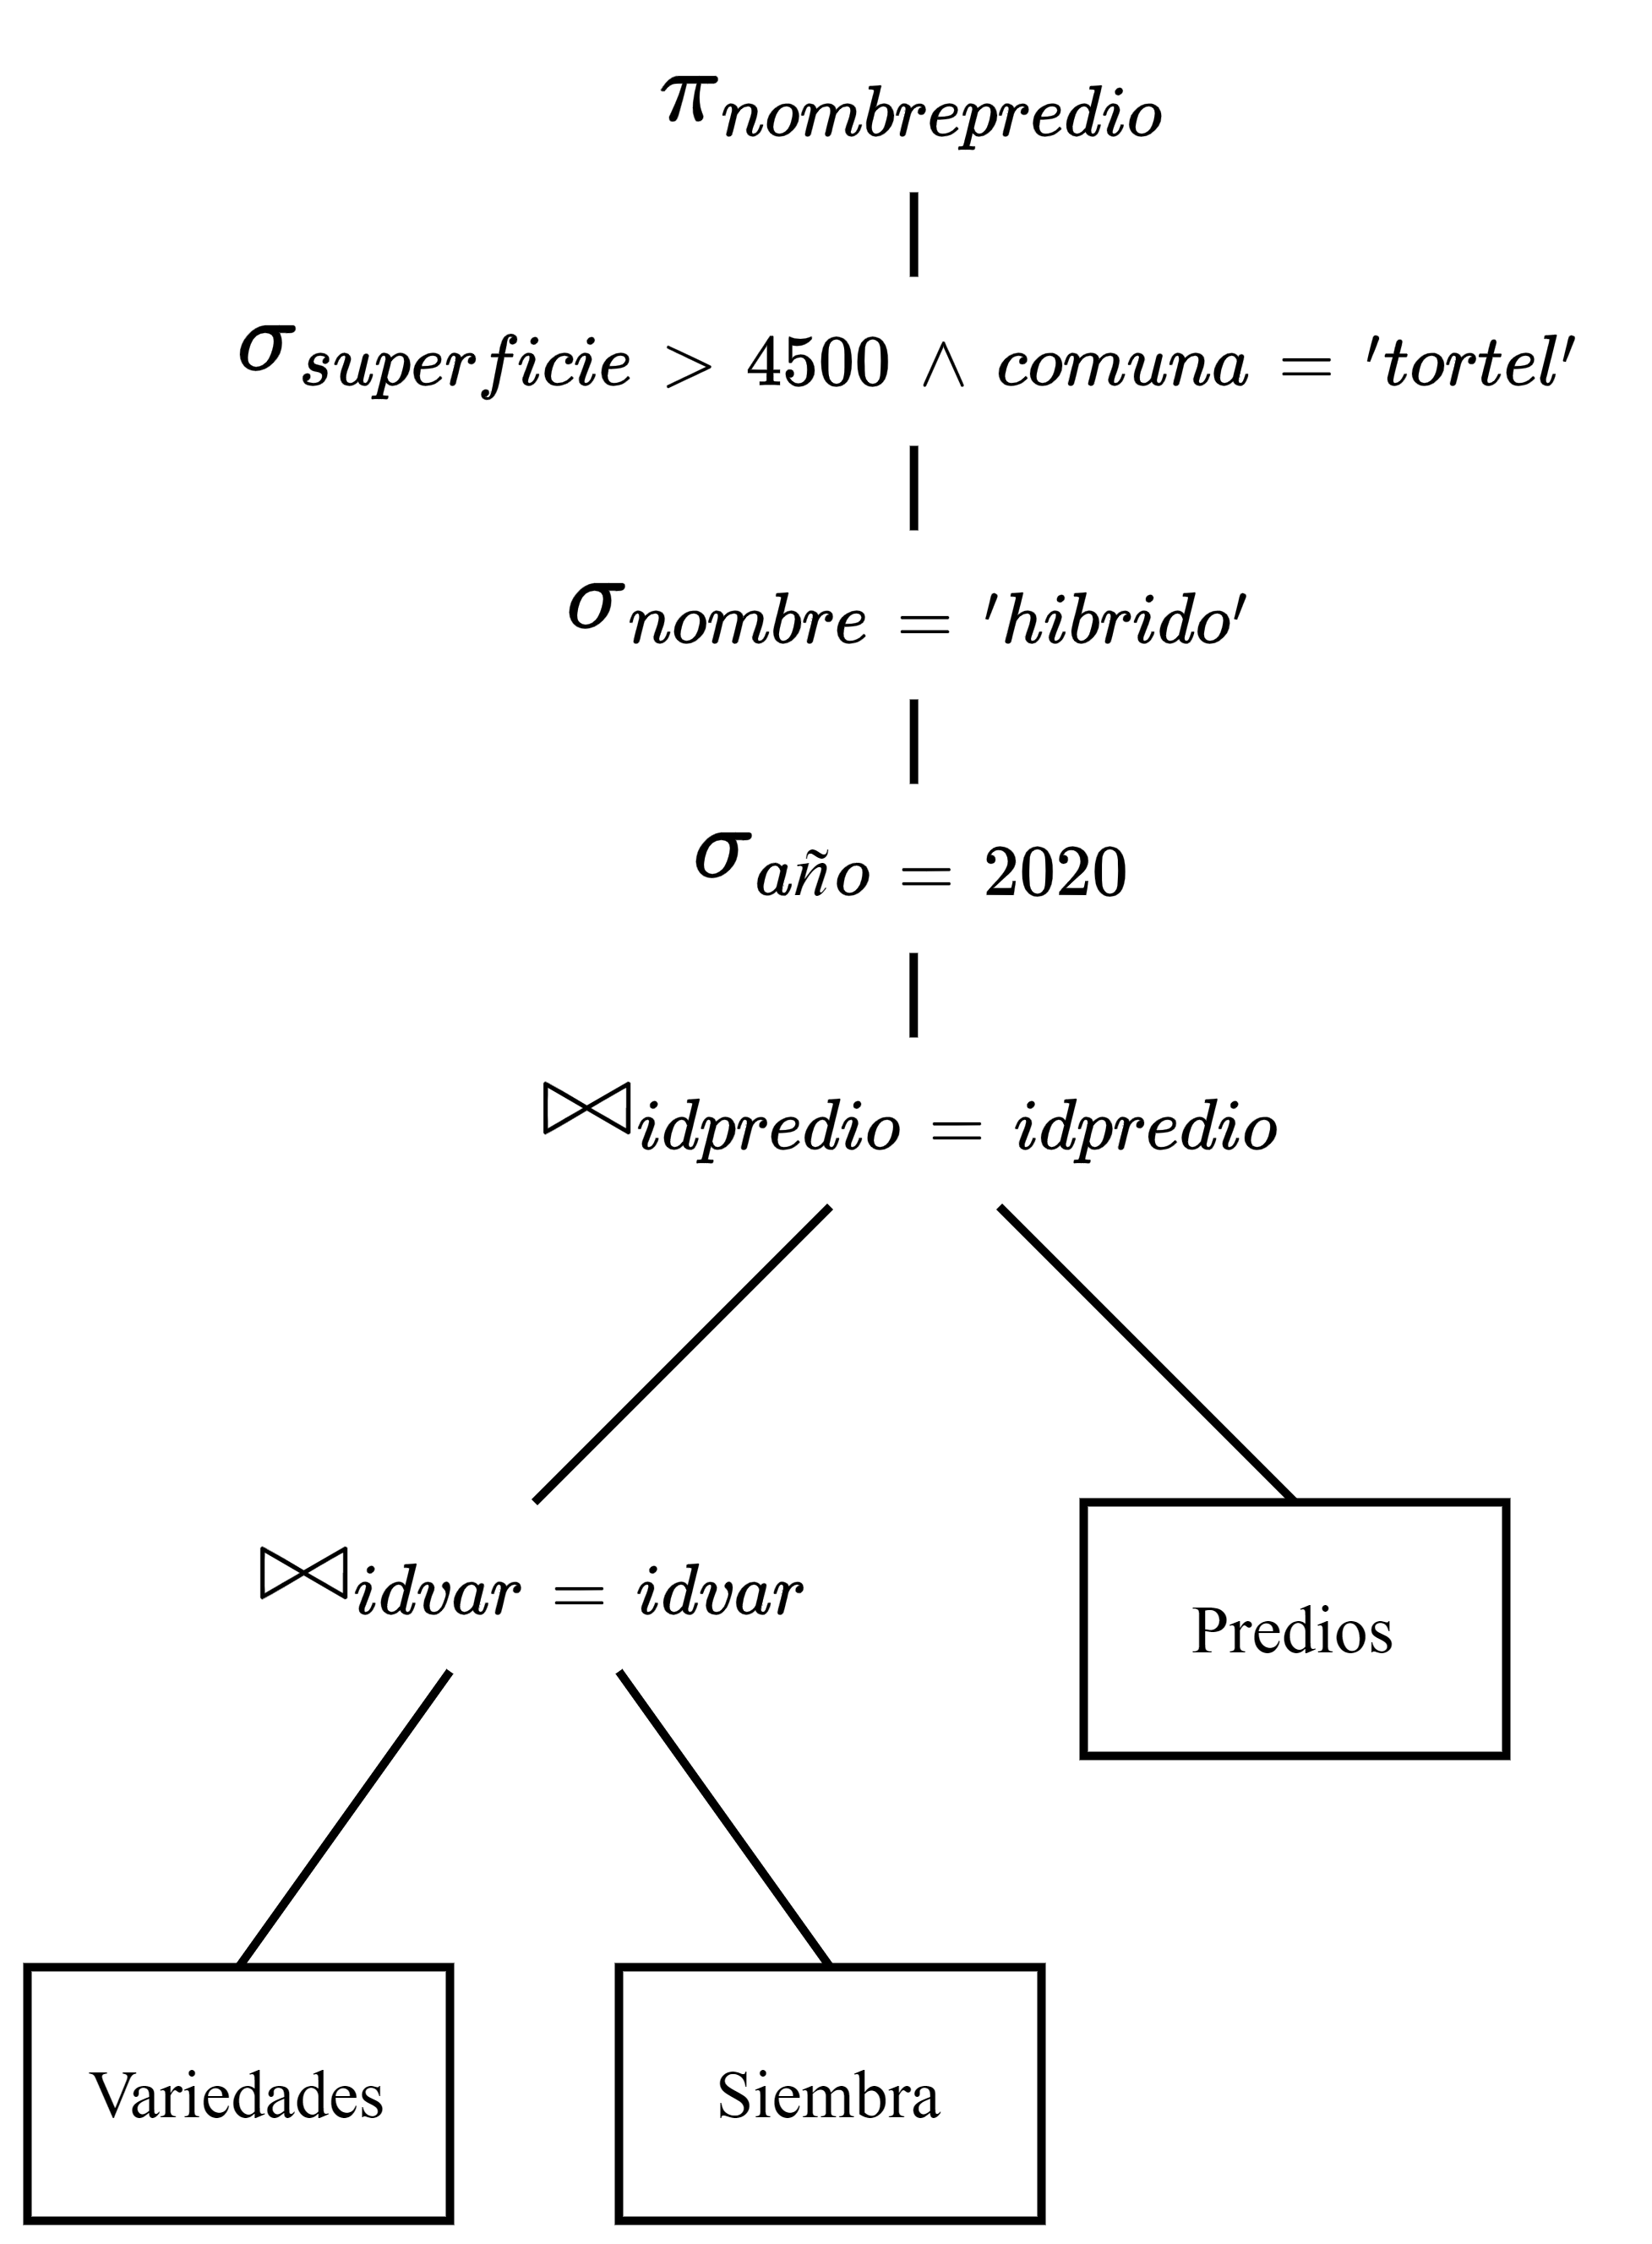
\includegraphics[width=0.5\textwidth]{img/E2-Paso-4.png}
            \end{figure}

            \item Bajar el resto de seleciones a tablas.
            \begin{figure}[H]
                \centering
                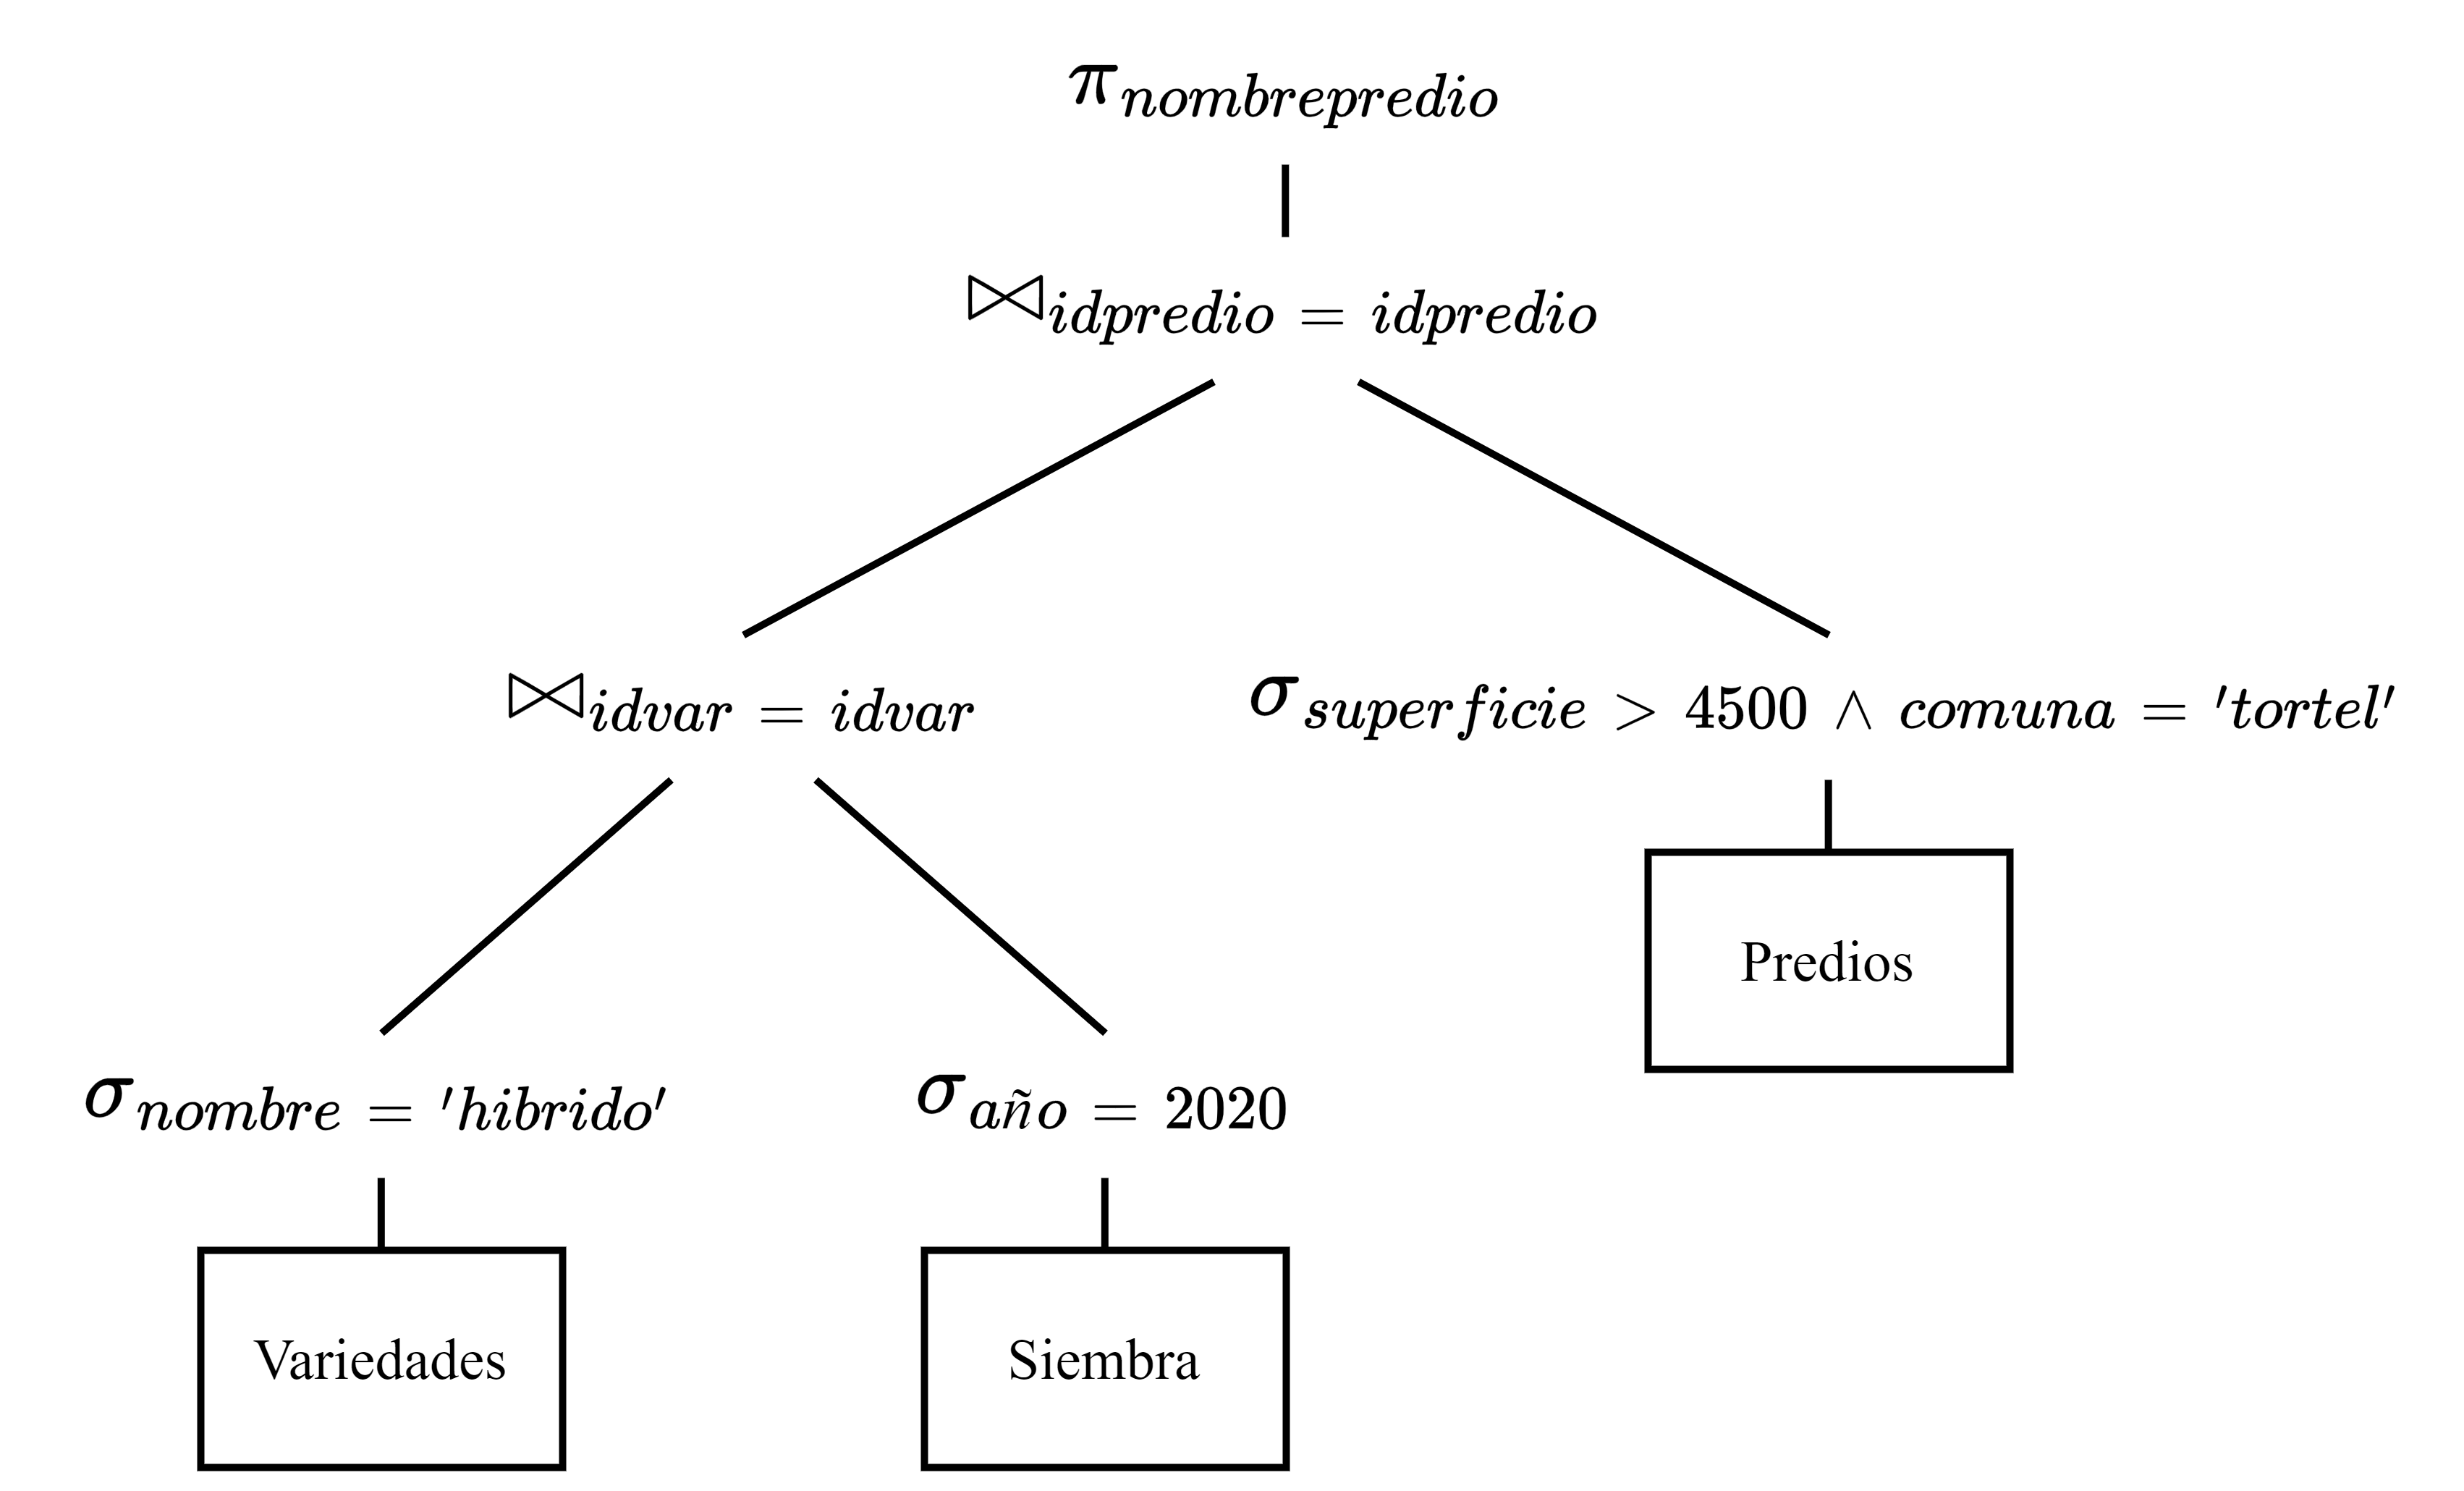
\includegraphics[width=\textwidth]{img/E2-Paso-5.png}
            \end{figure}

            \newpage
            \item Proyectar los atributos necesarios.
            \begin{figure}[H]
                \centering
                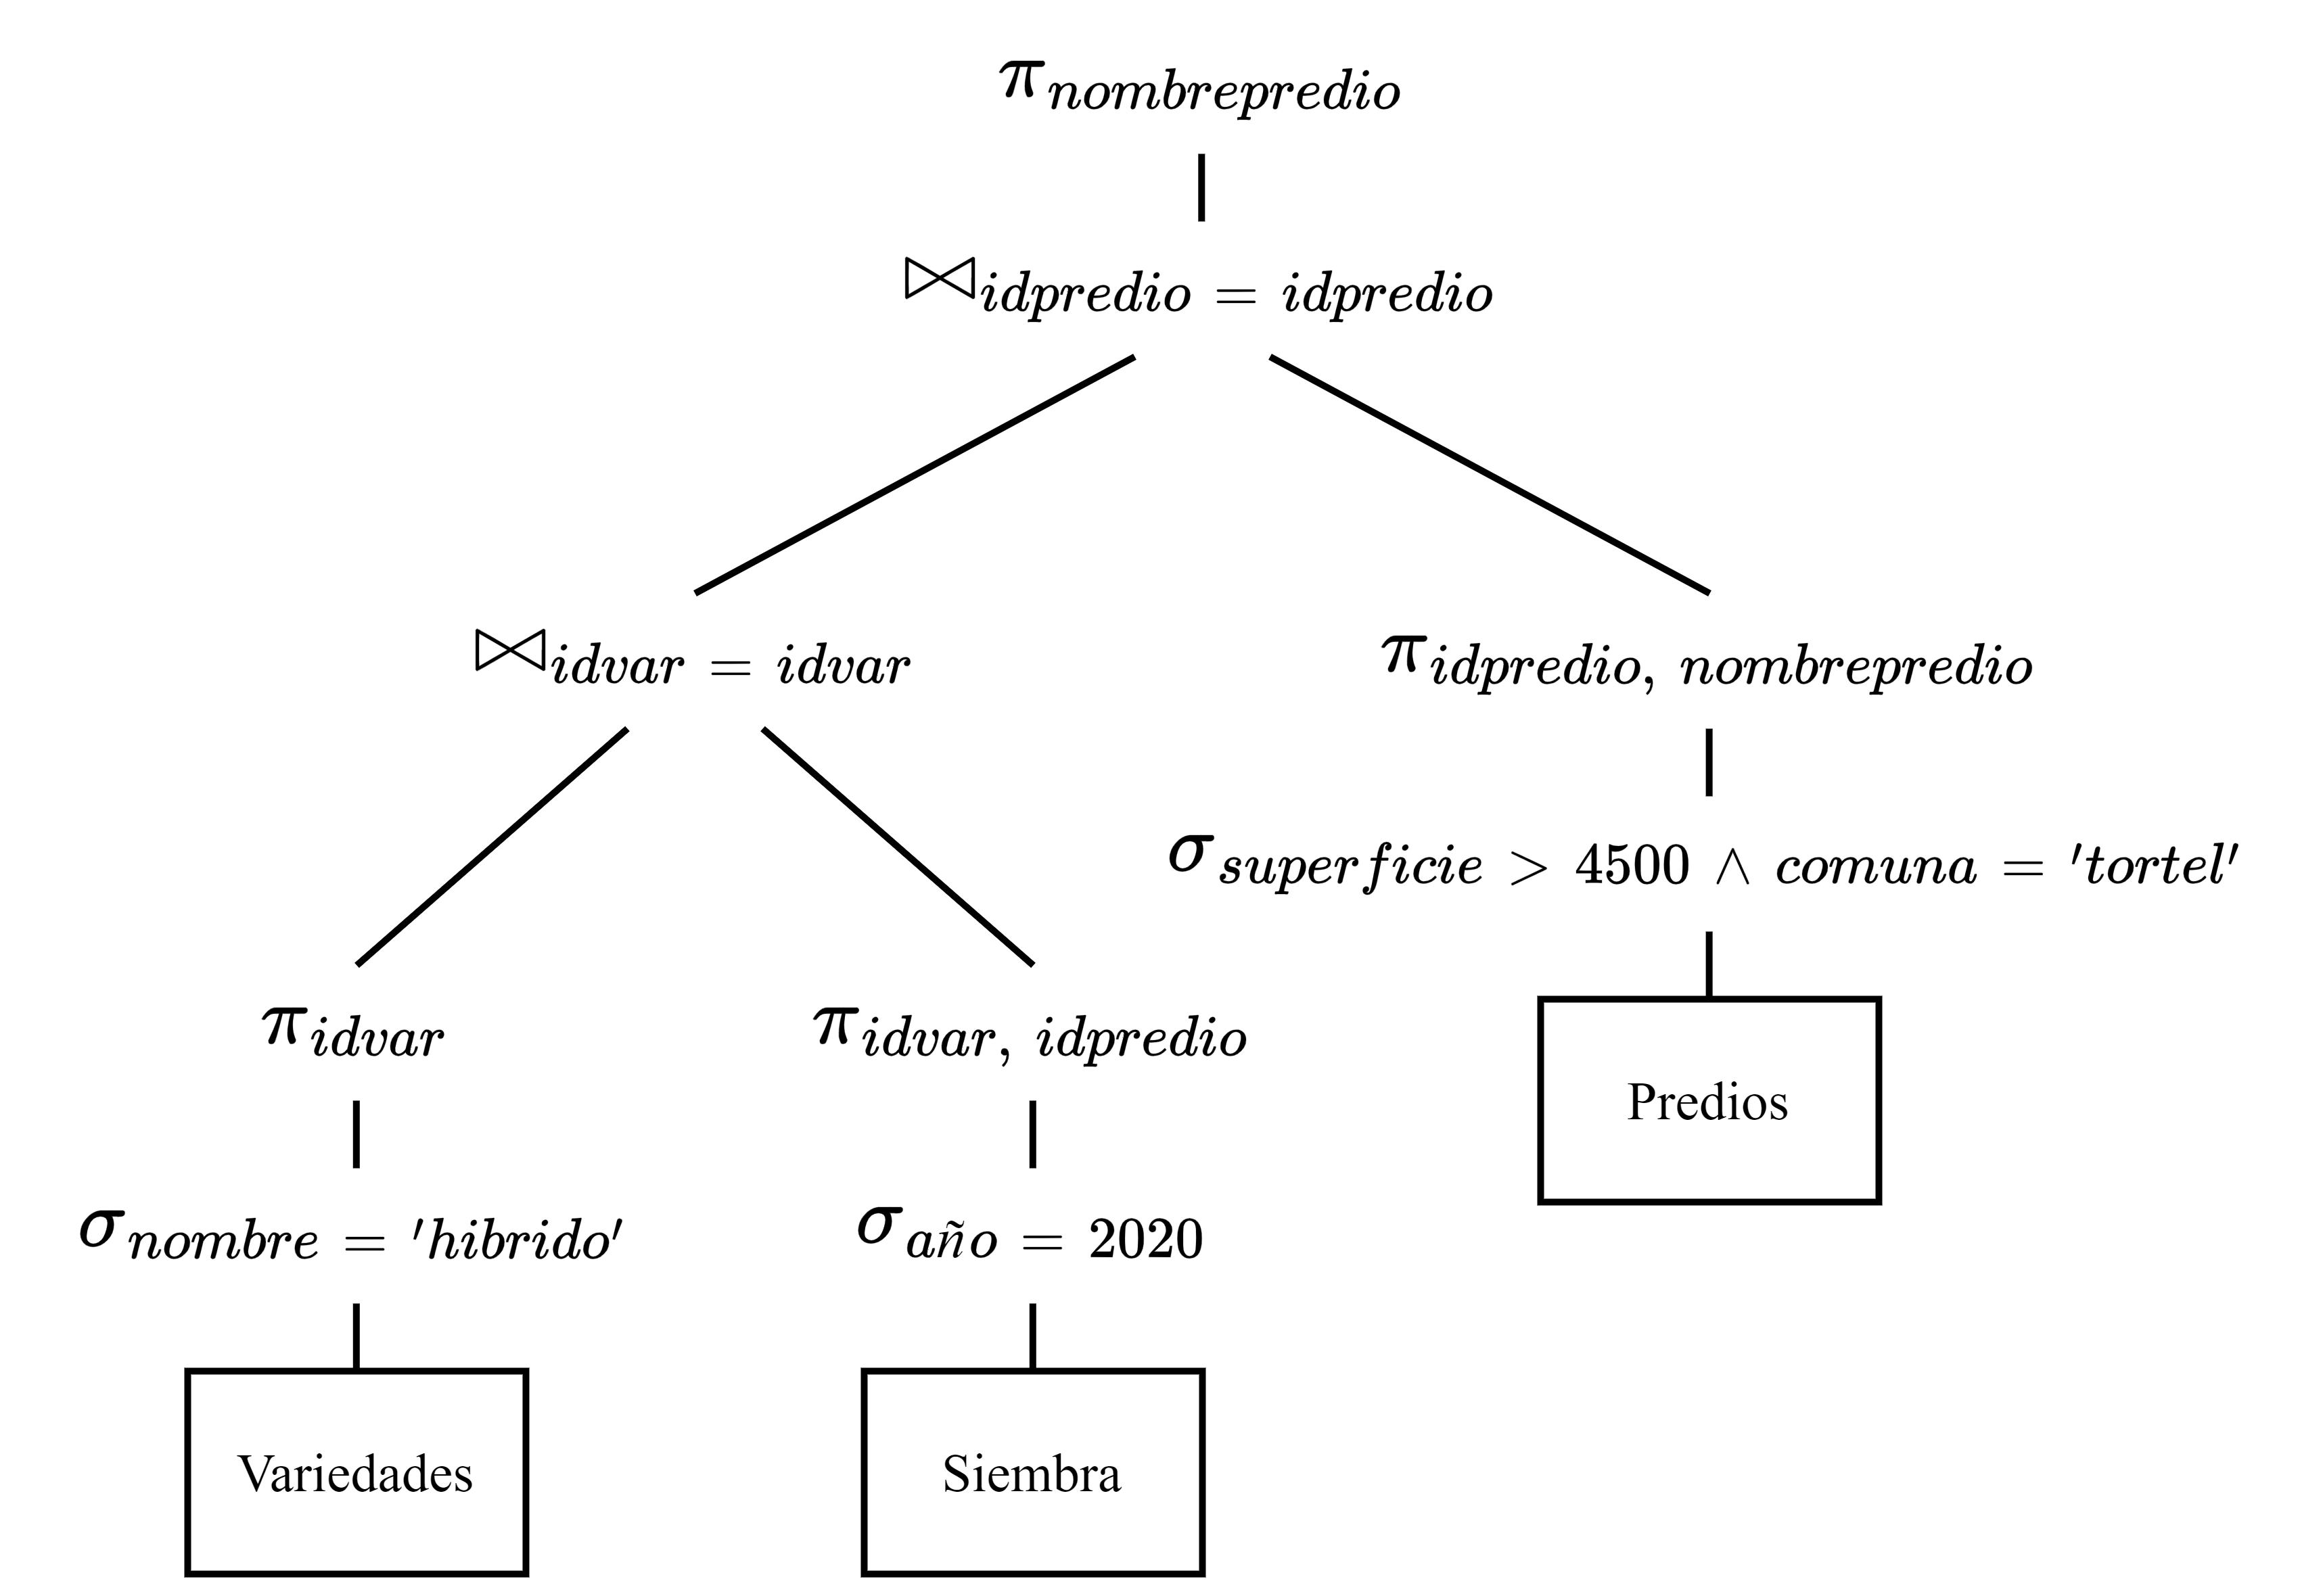
\includegraphics[width=\textwidth]{img/E2-Paso-6.png}
            \end{figure}
        \end{enumerate}
    \end{itemize}

    \newpage
    \item \'Arbol Can\'onico.
    \begin{figure}[H]
        \centering
        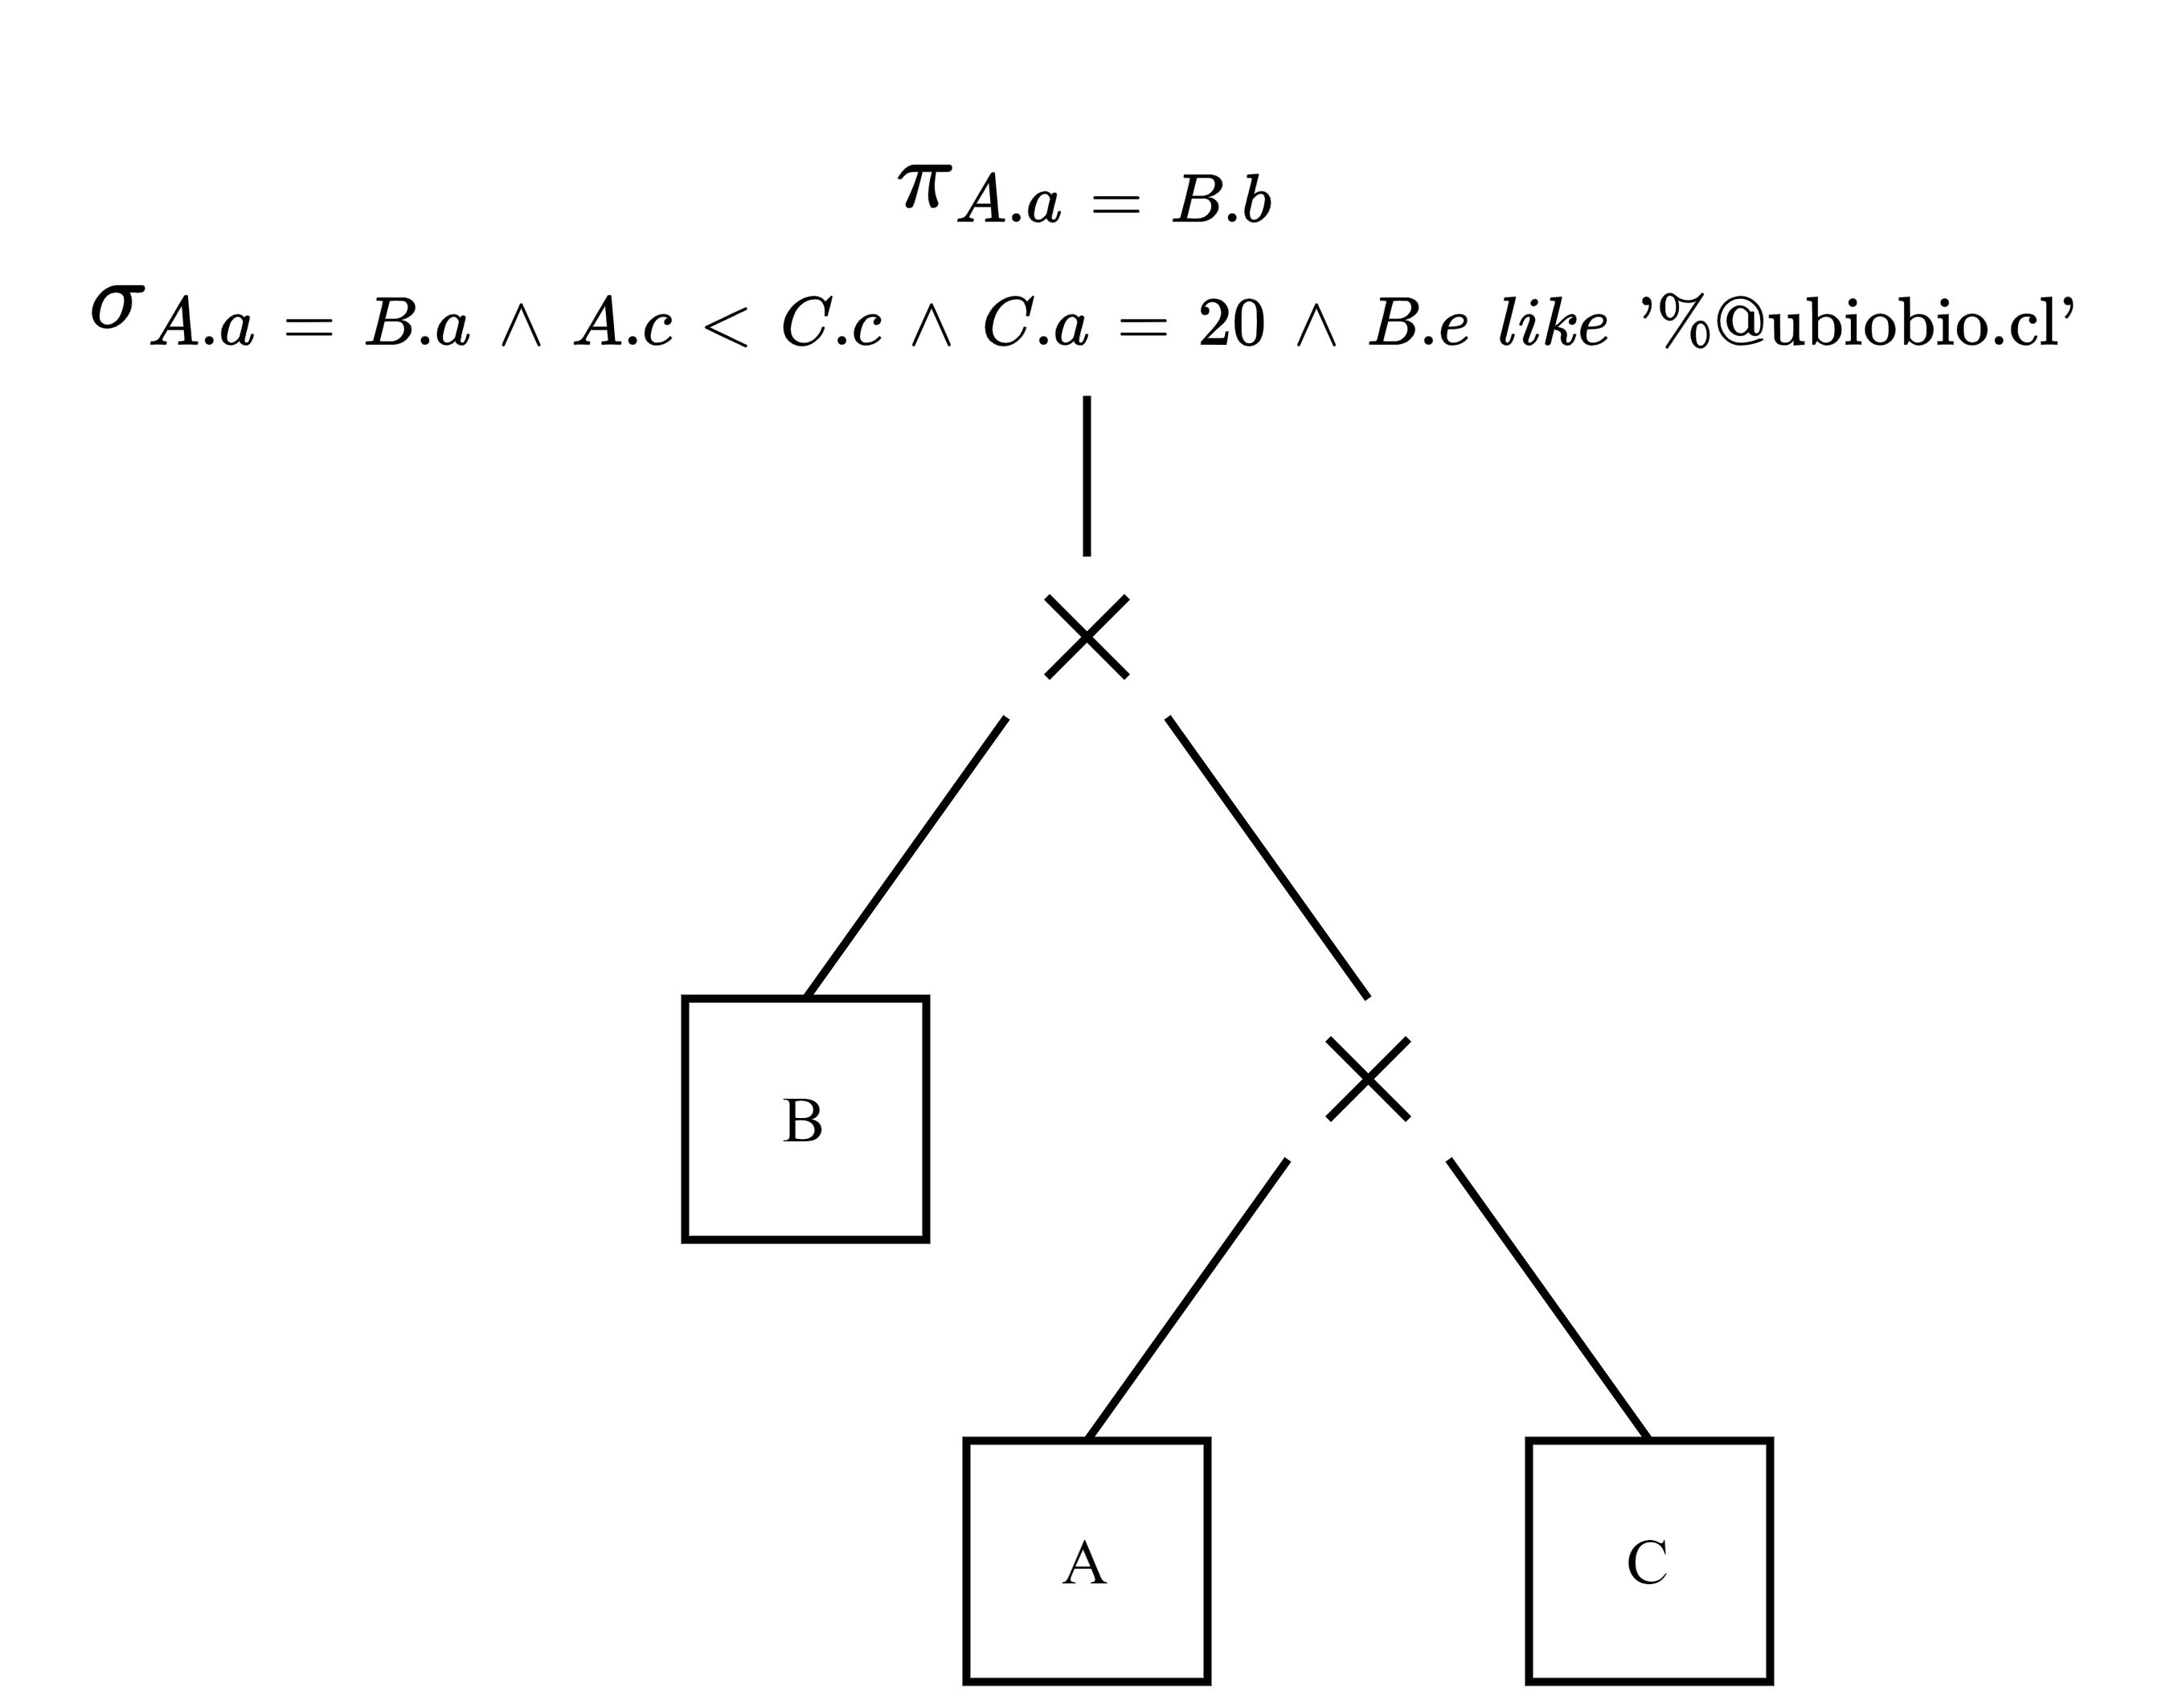
\includegraphics[width=0.65\textwidth]{img/E3-Canonico.png}
    \end{figure}

    \begin{itemize}
        \item Optimizar
        \begin{enumerate}
            \item Separar las selecciones.
            \begin{figure}[H]
                \centering
                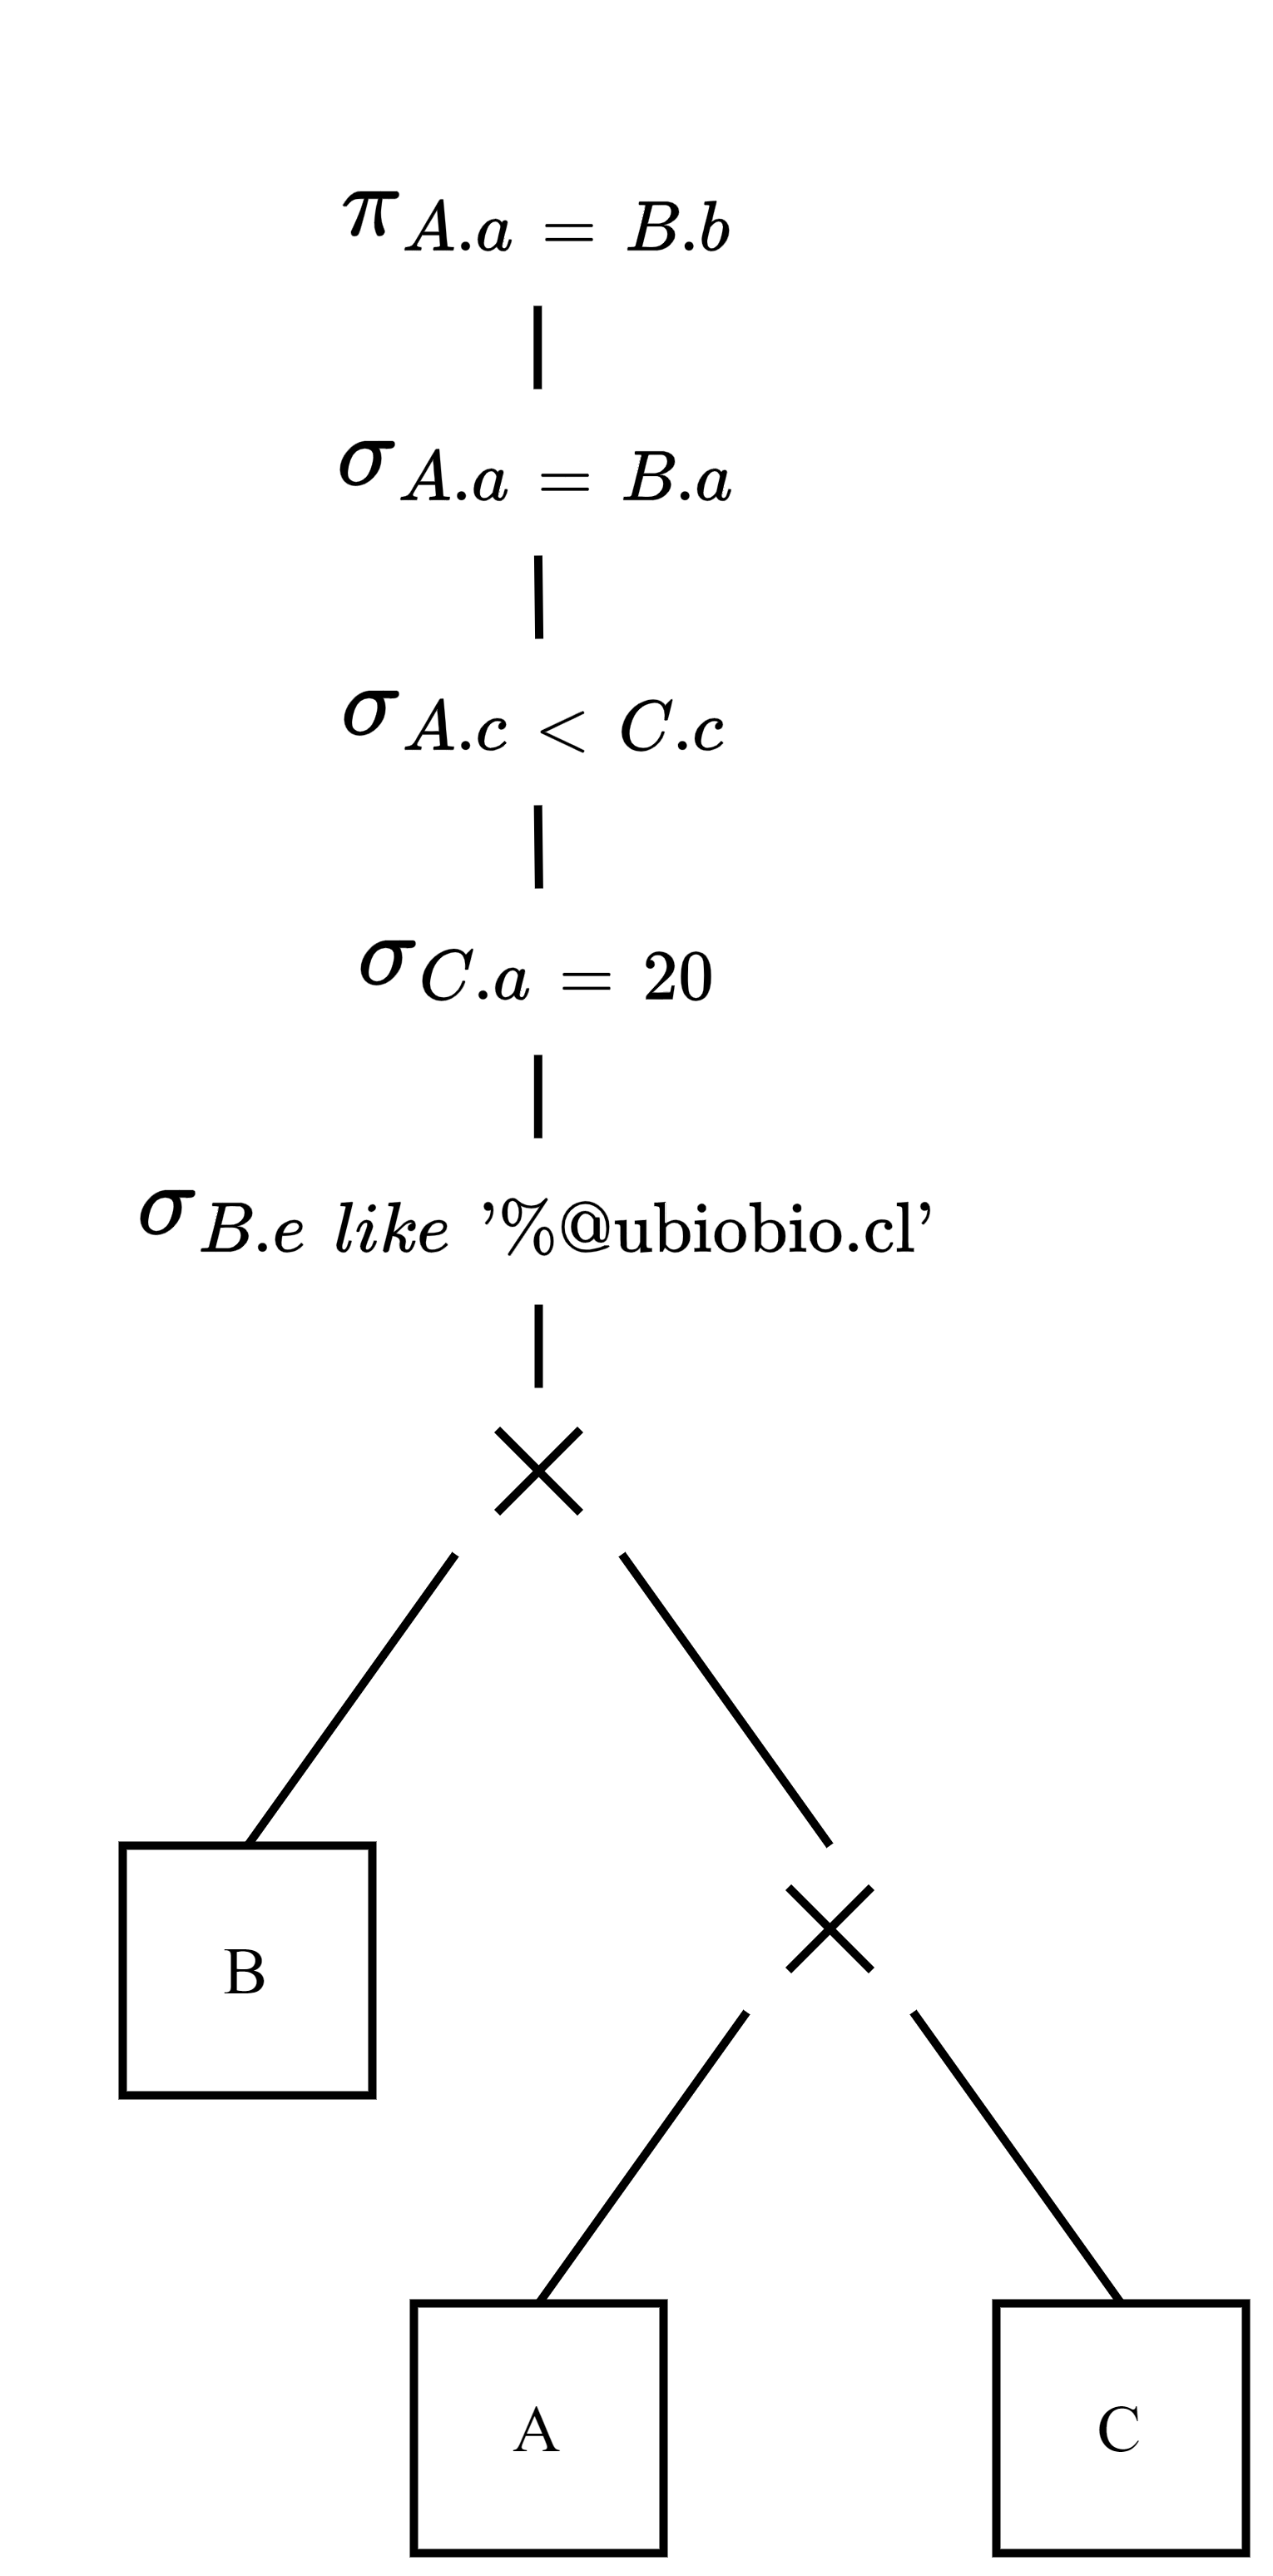
\includegraphics[width=0.4\textwidth]{img/E3-Paso-1.png}
            \end{figure}

            \newpage
            \item Permutar tablas si es necesario.

            \item Bajar las seleciones que son $\times$ para $\Join$.
            \begin{figure}[H]
                \centering
                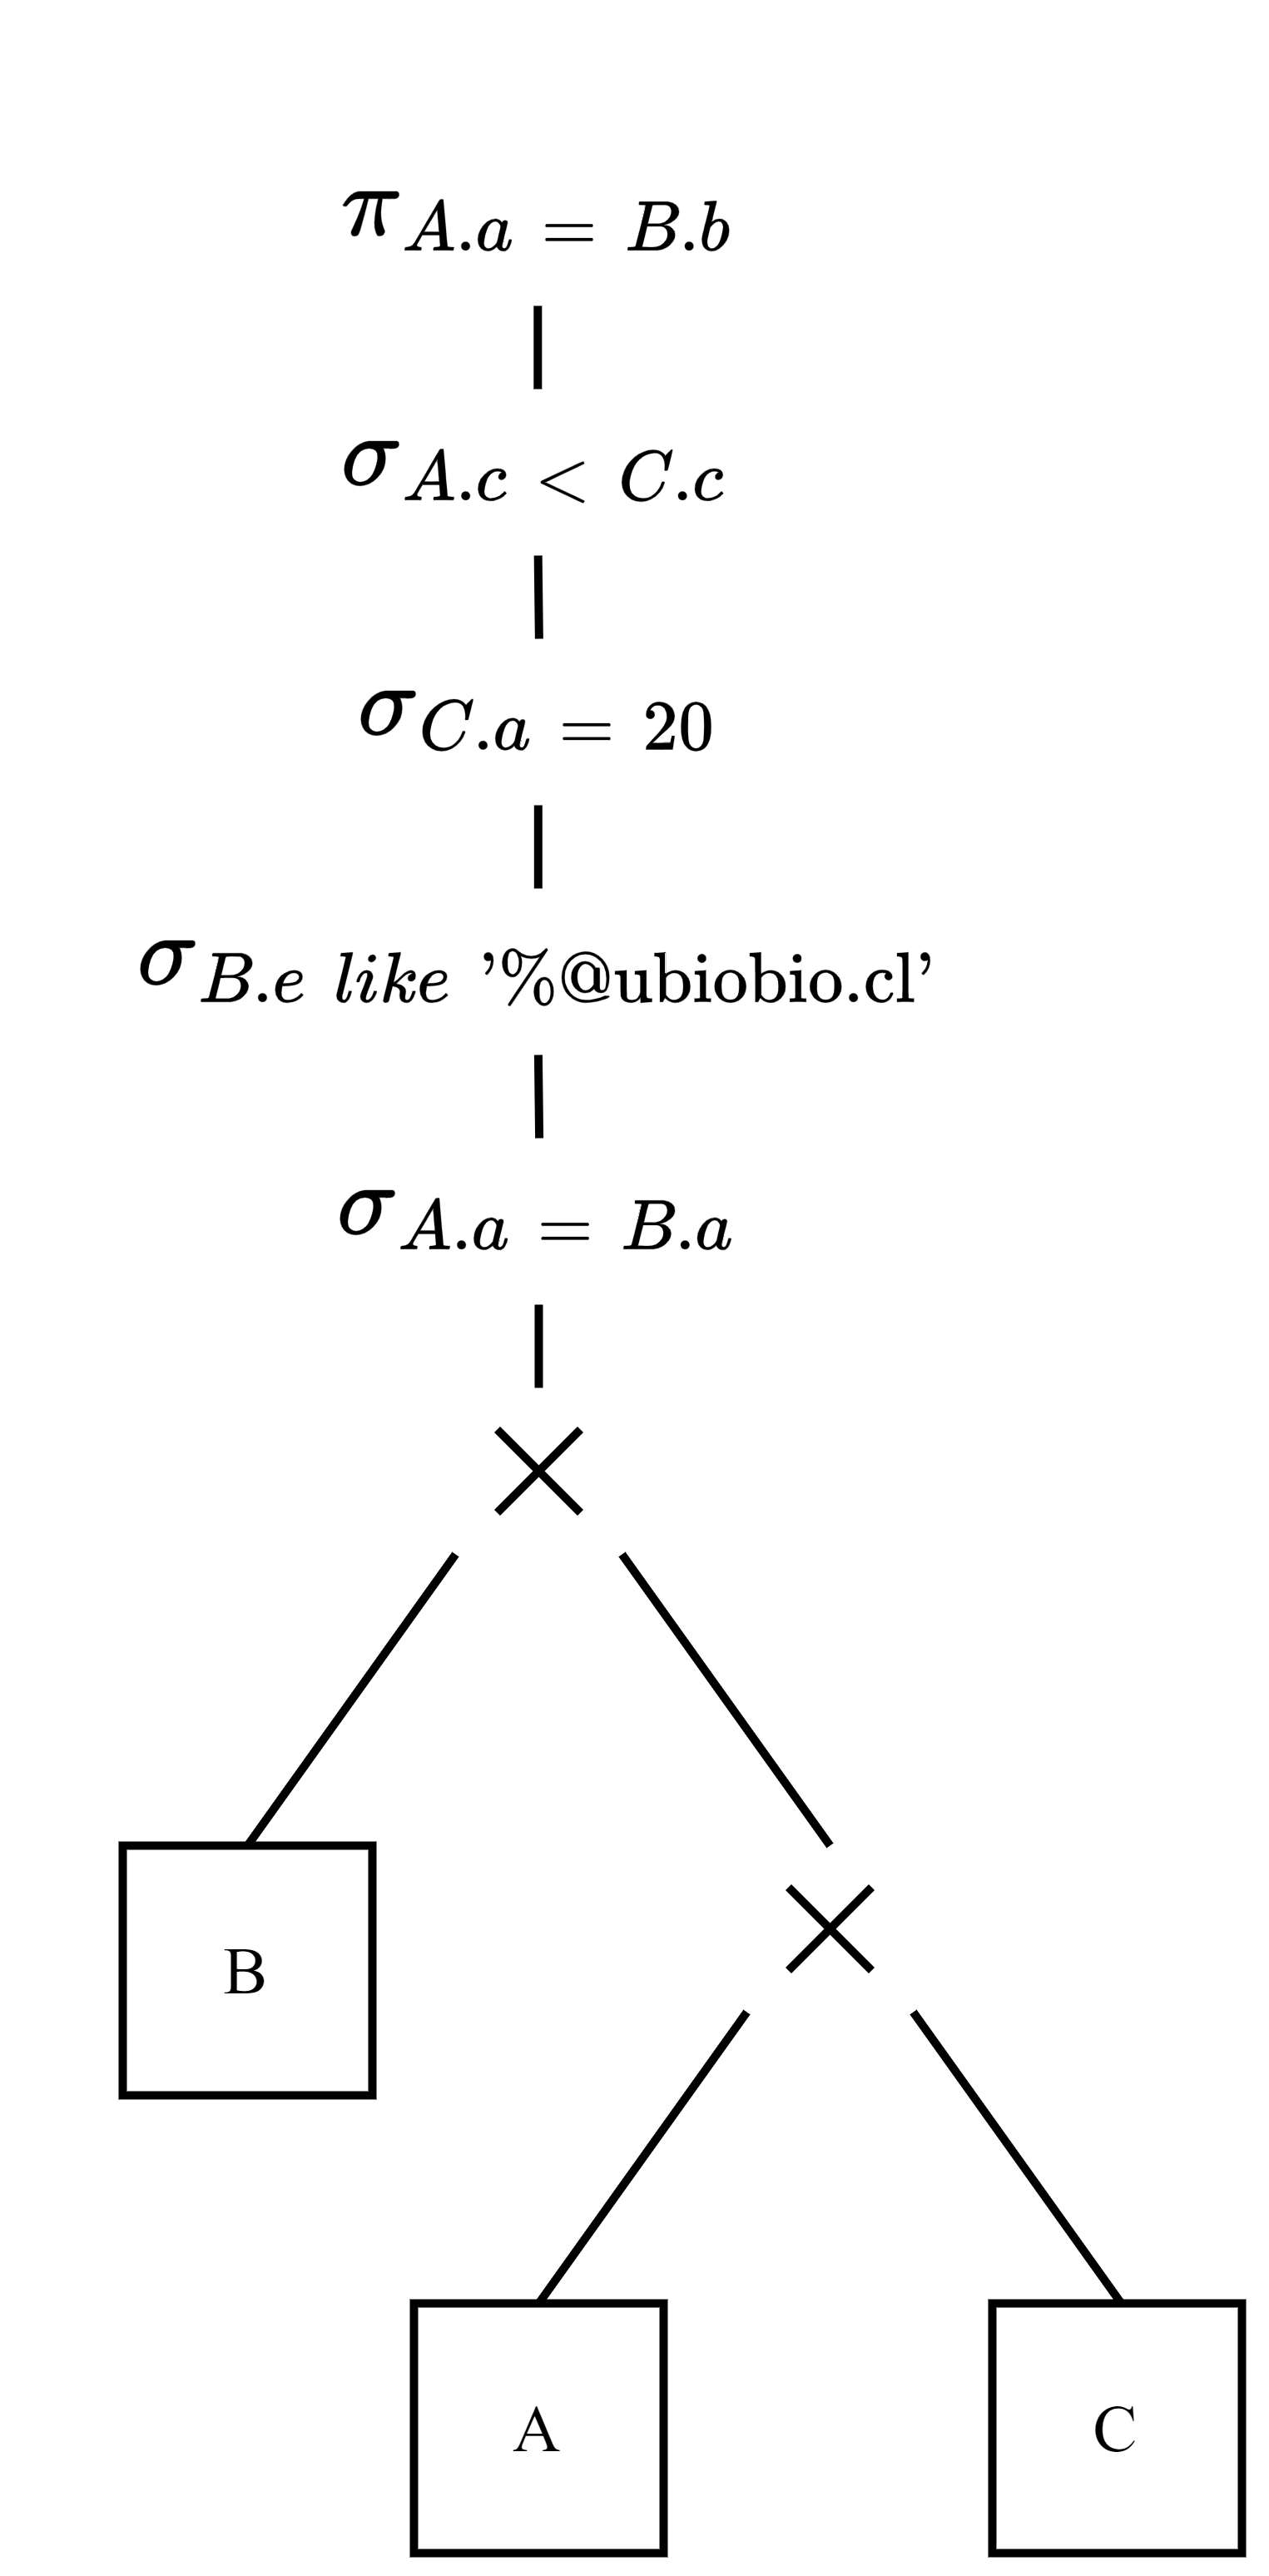
\includegraphics[width=0.345\textwidth]{img/E3-Paso-3.png}
            \end{figure}

            \item Cambio $\times$ por $\Join$.
            \begin{figure}[H]
                \centering
                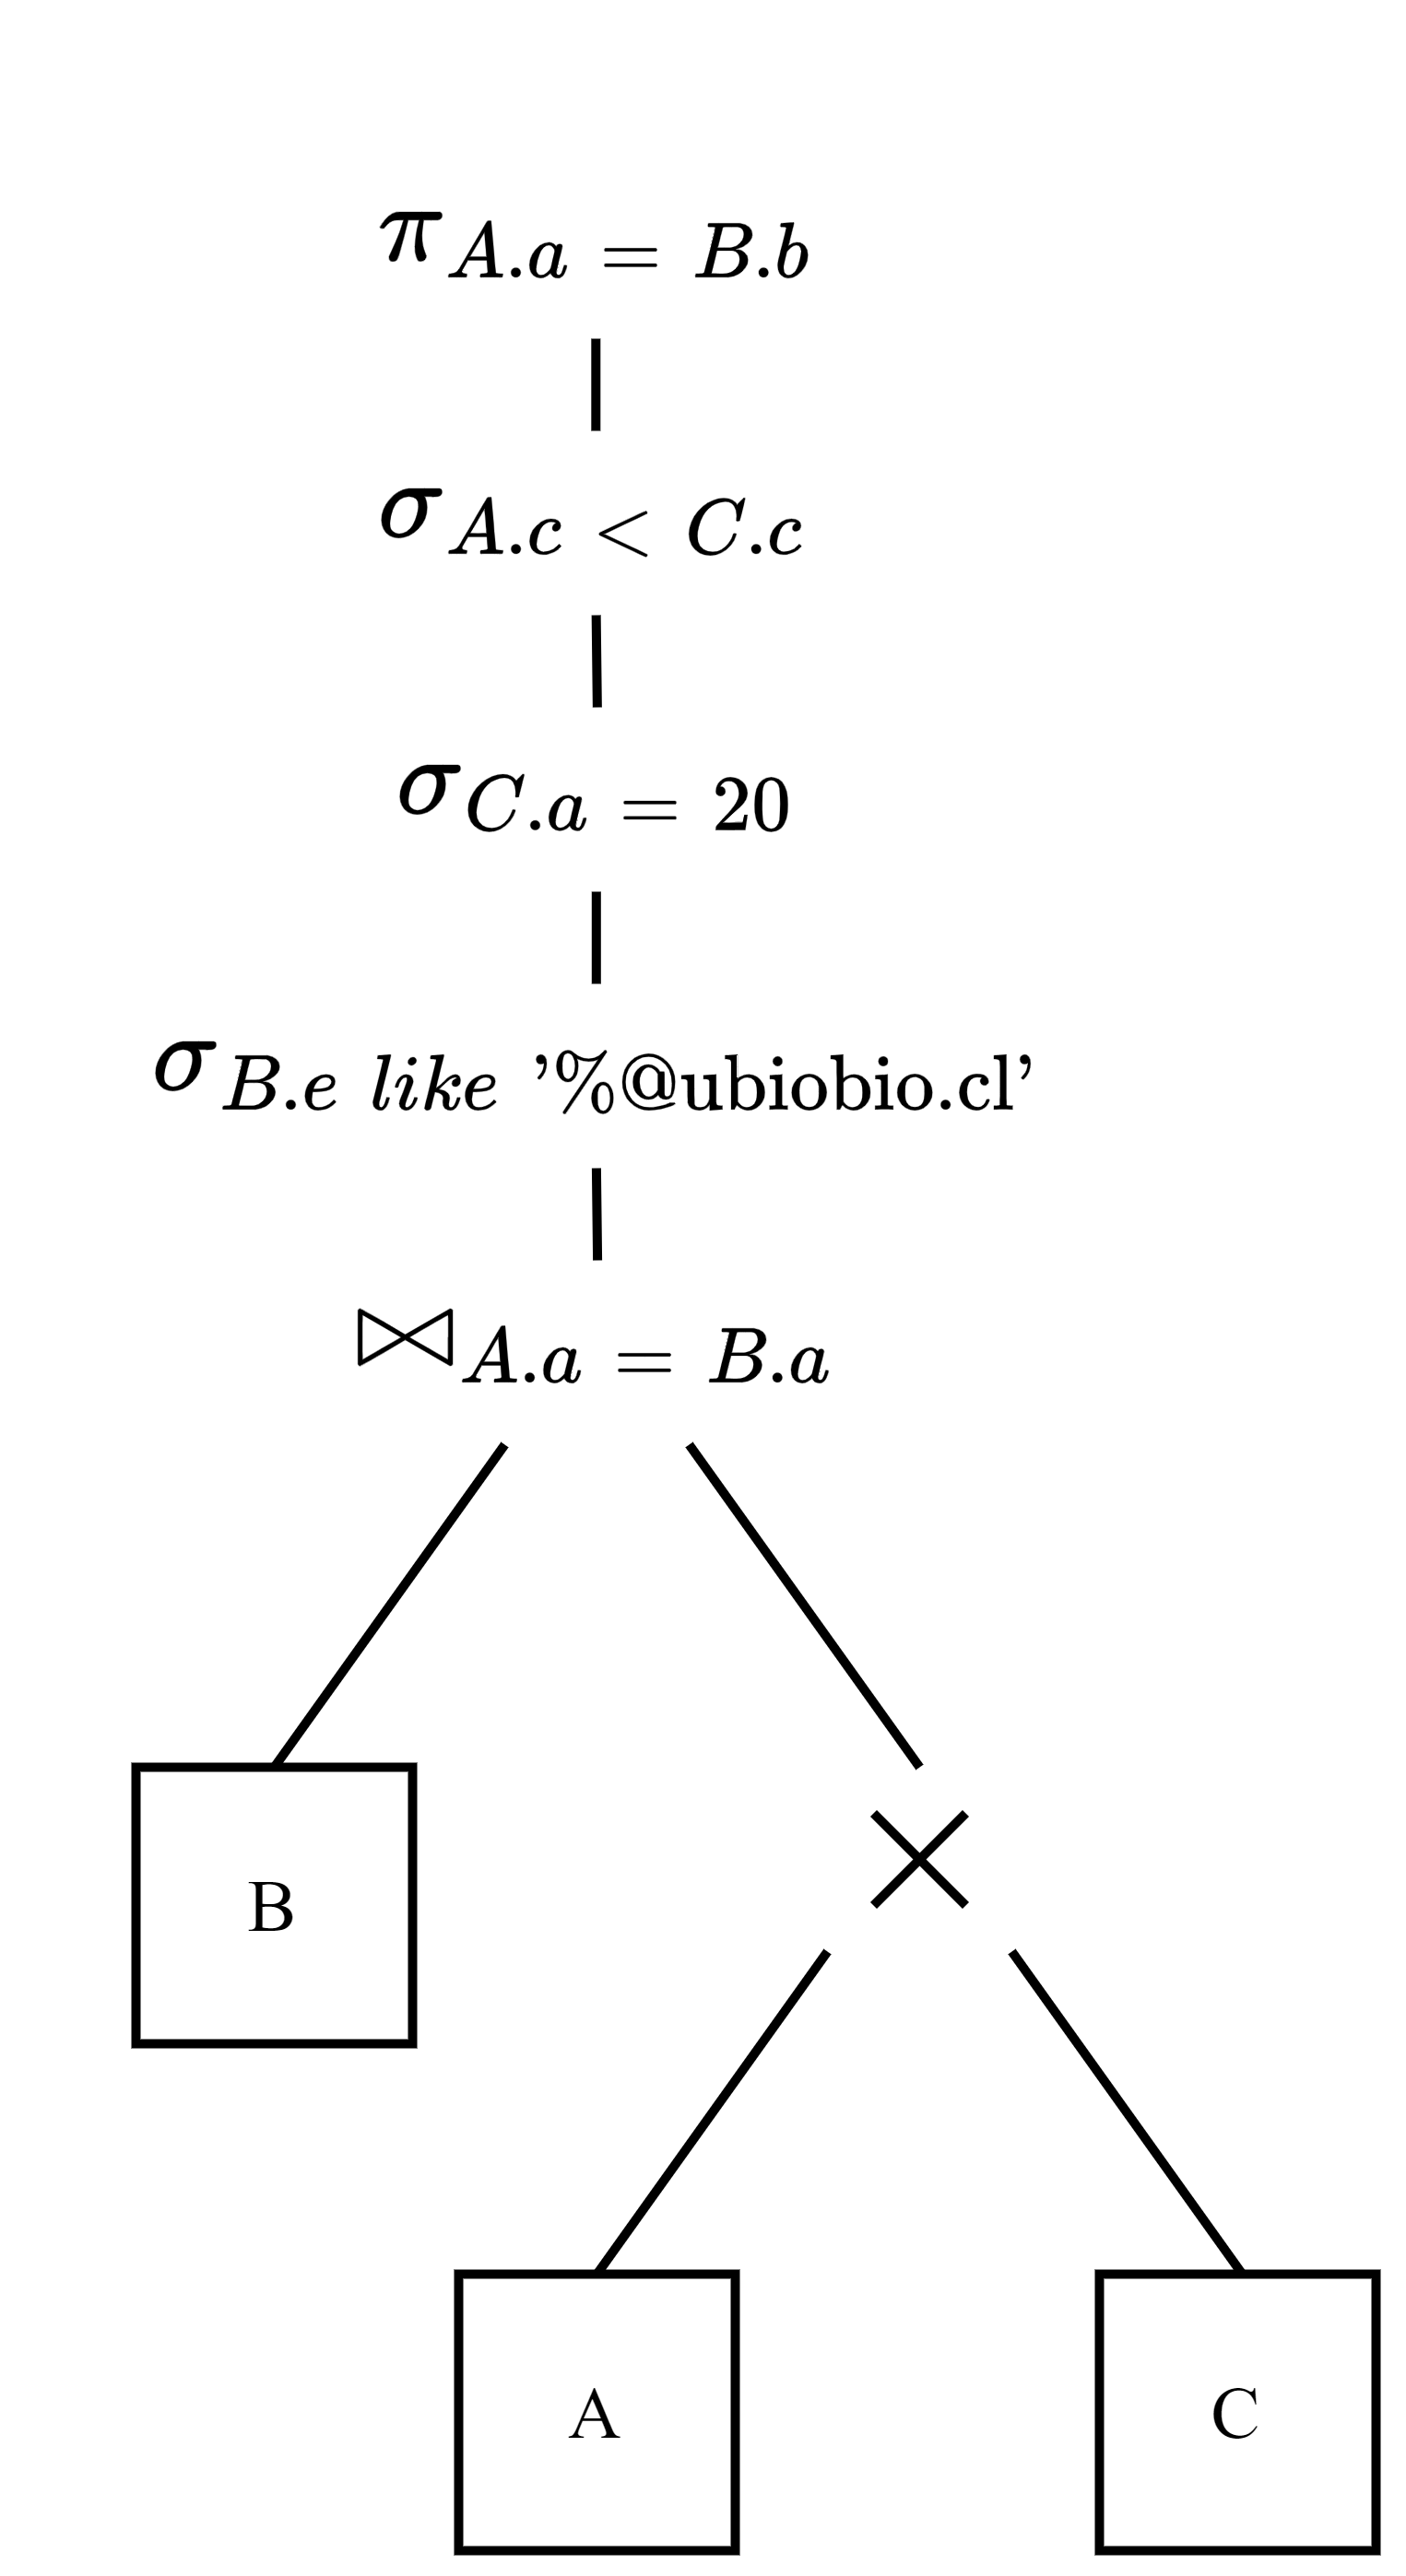
\includegraphics[width=0.345\textwidth]{img/E3-Paso-4.png}
            \end{figure}

            \newpage
            \item Bajar el resto de seleciones a tablas.
            \begin{figure}[H]
                \centering
                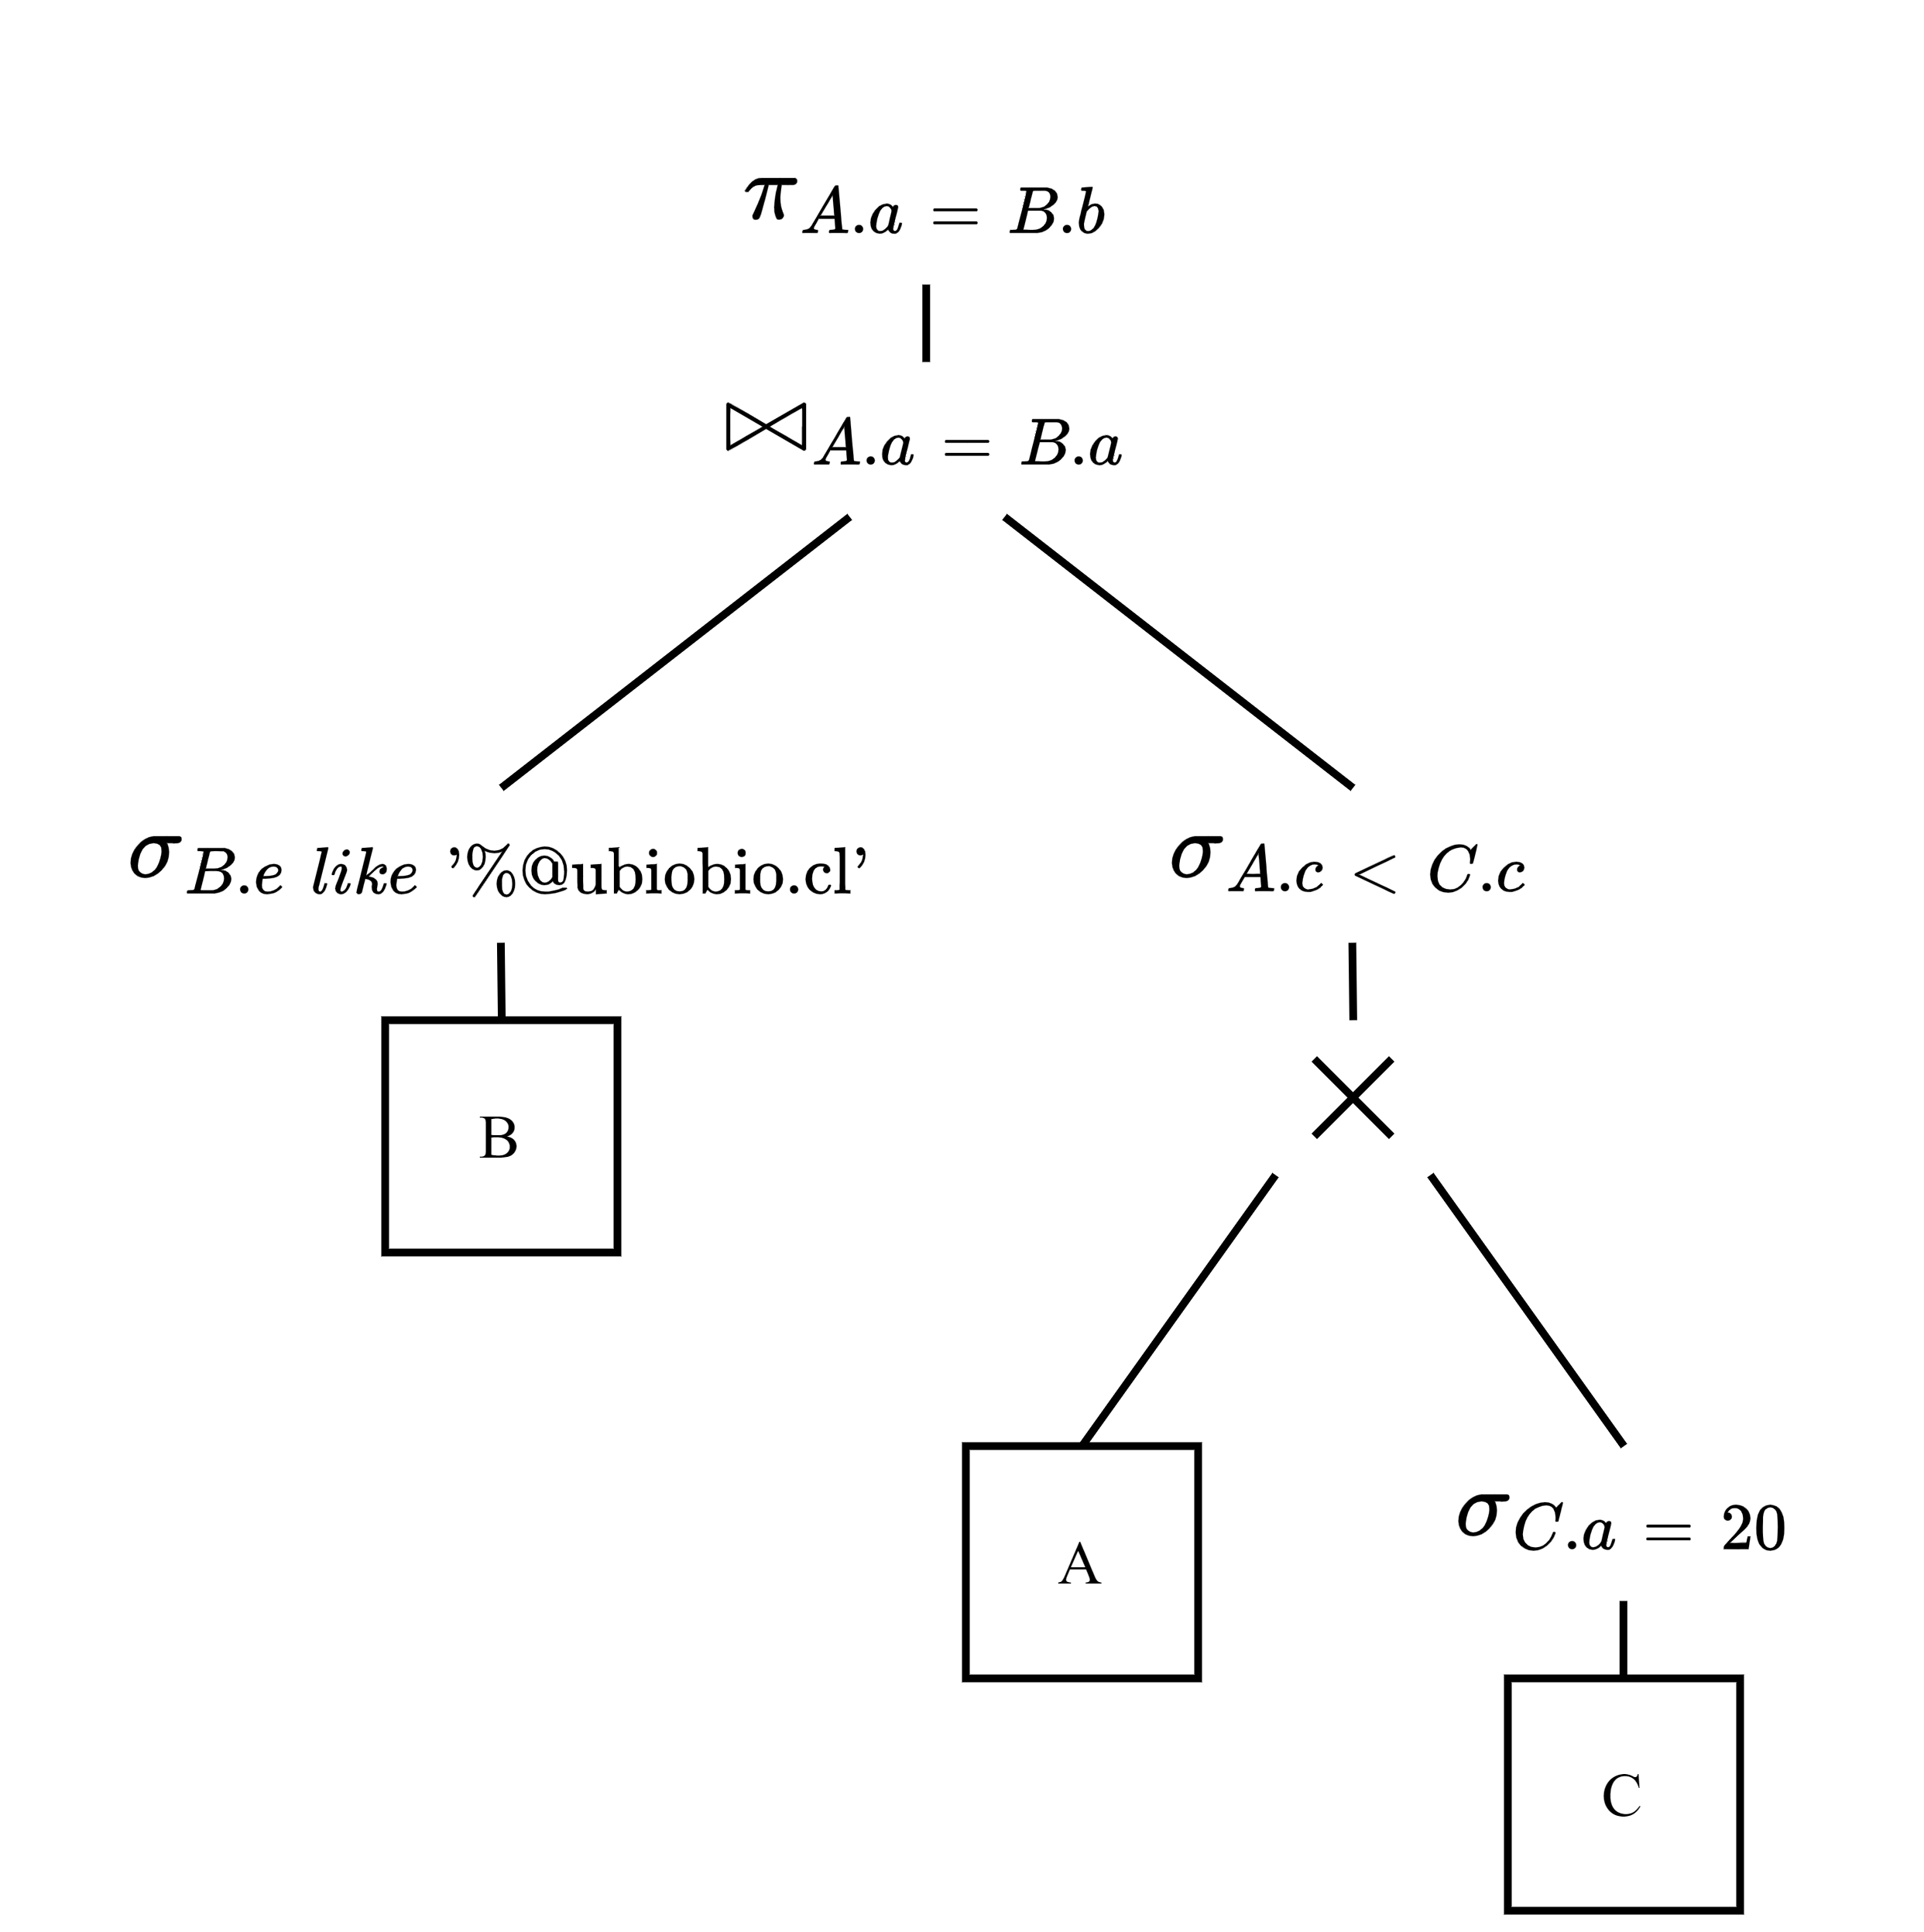
\includegraphics[width=0.55\textwidth]{img/E3-Paso-5.png}
            \end{figure}

            \item Proyectar los atributos necesarios.
            \begin{figure}[H]
                \centering
                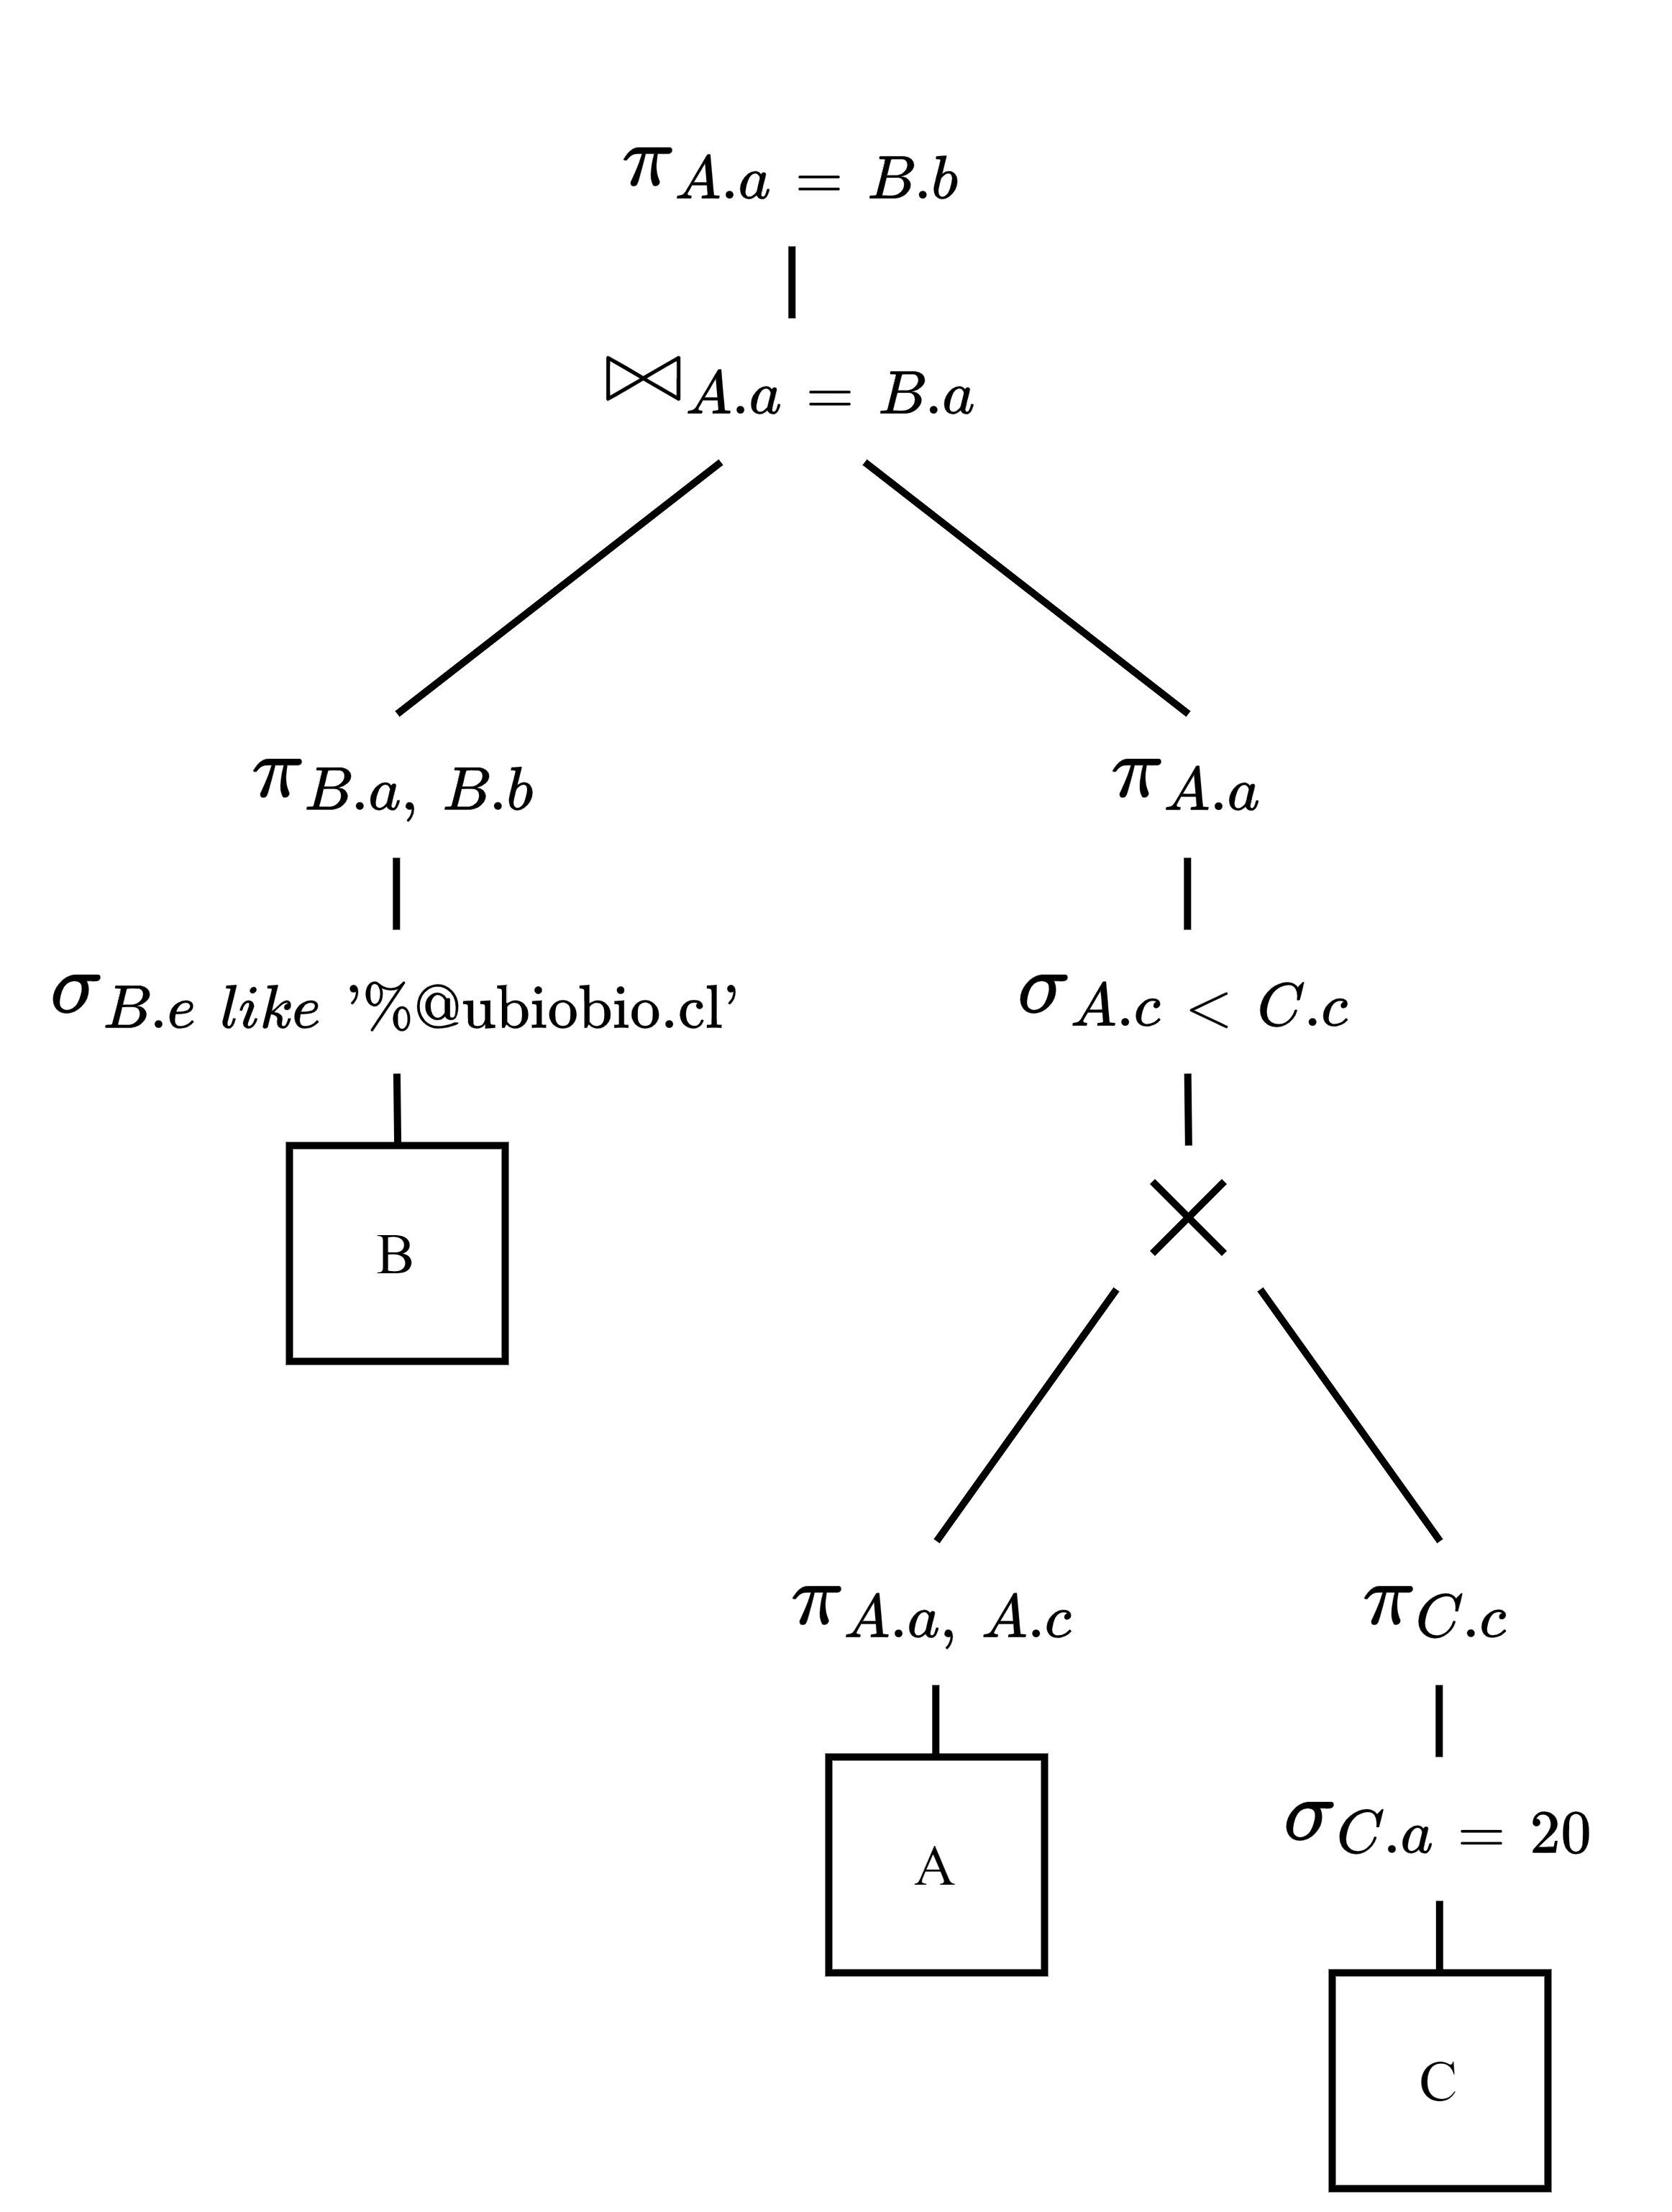
\includegraphics[width=0.55\textwidth]{img/E3-Paso-6.png}
            \end{figure}
        \end{enumerate}
    \end{itemize}

    \newpage
    \item \'Arbol Can\'onico.
    \begin{figure}[H]
        \centering
        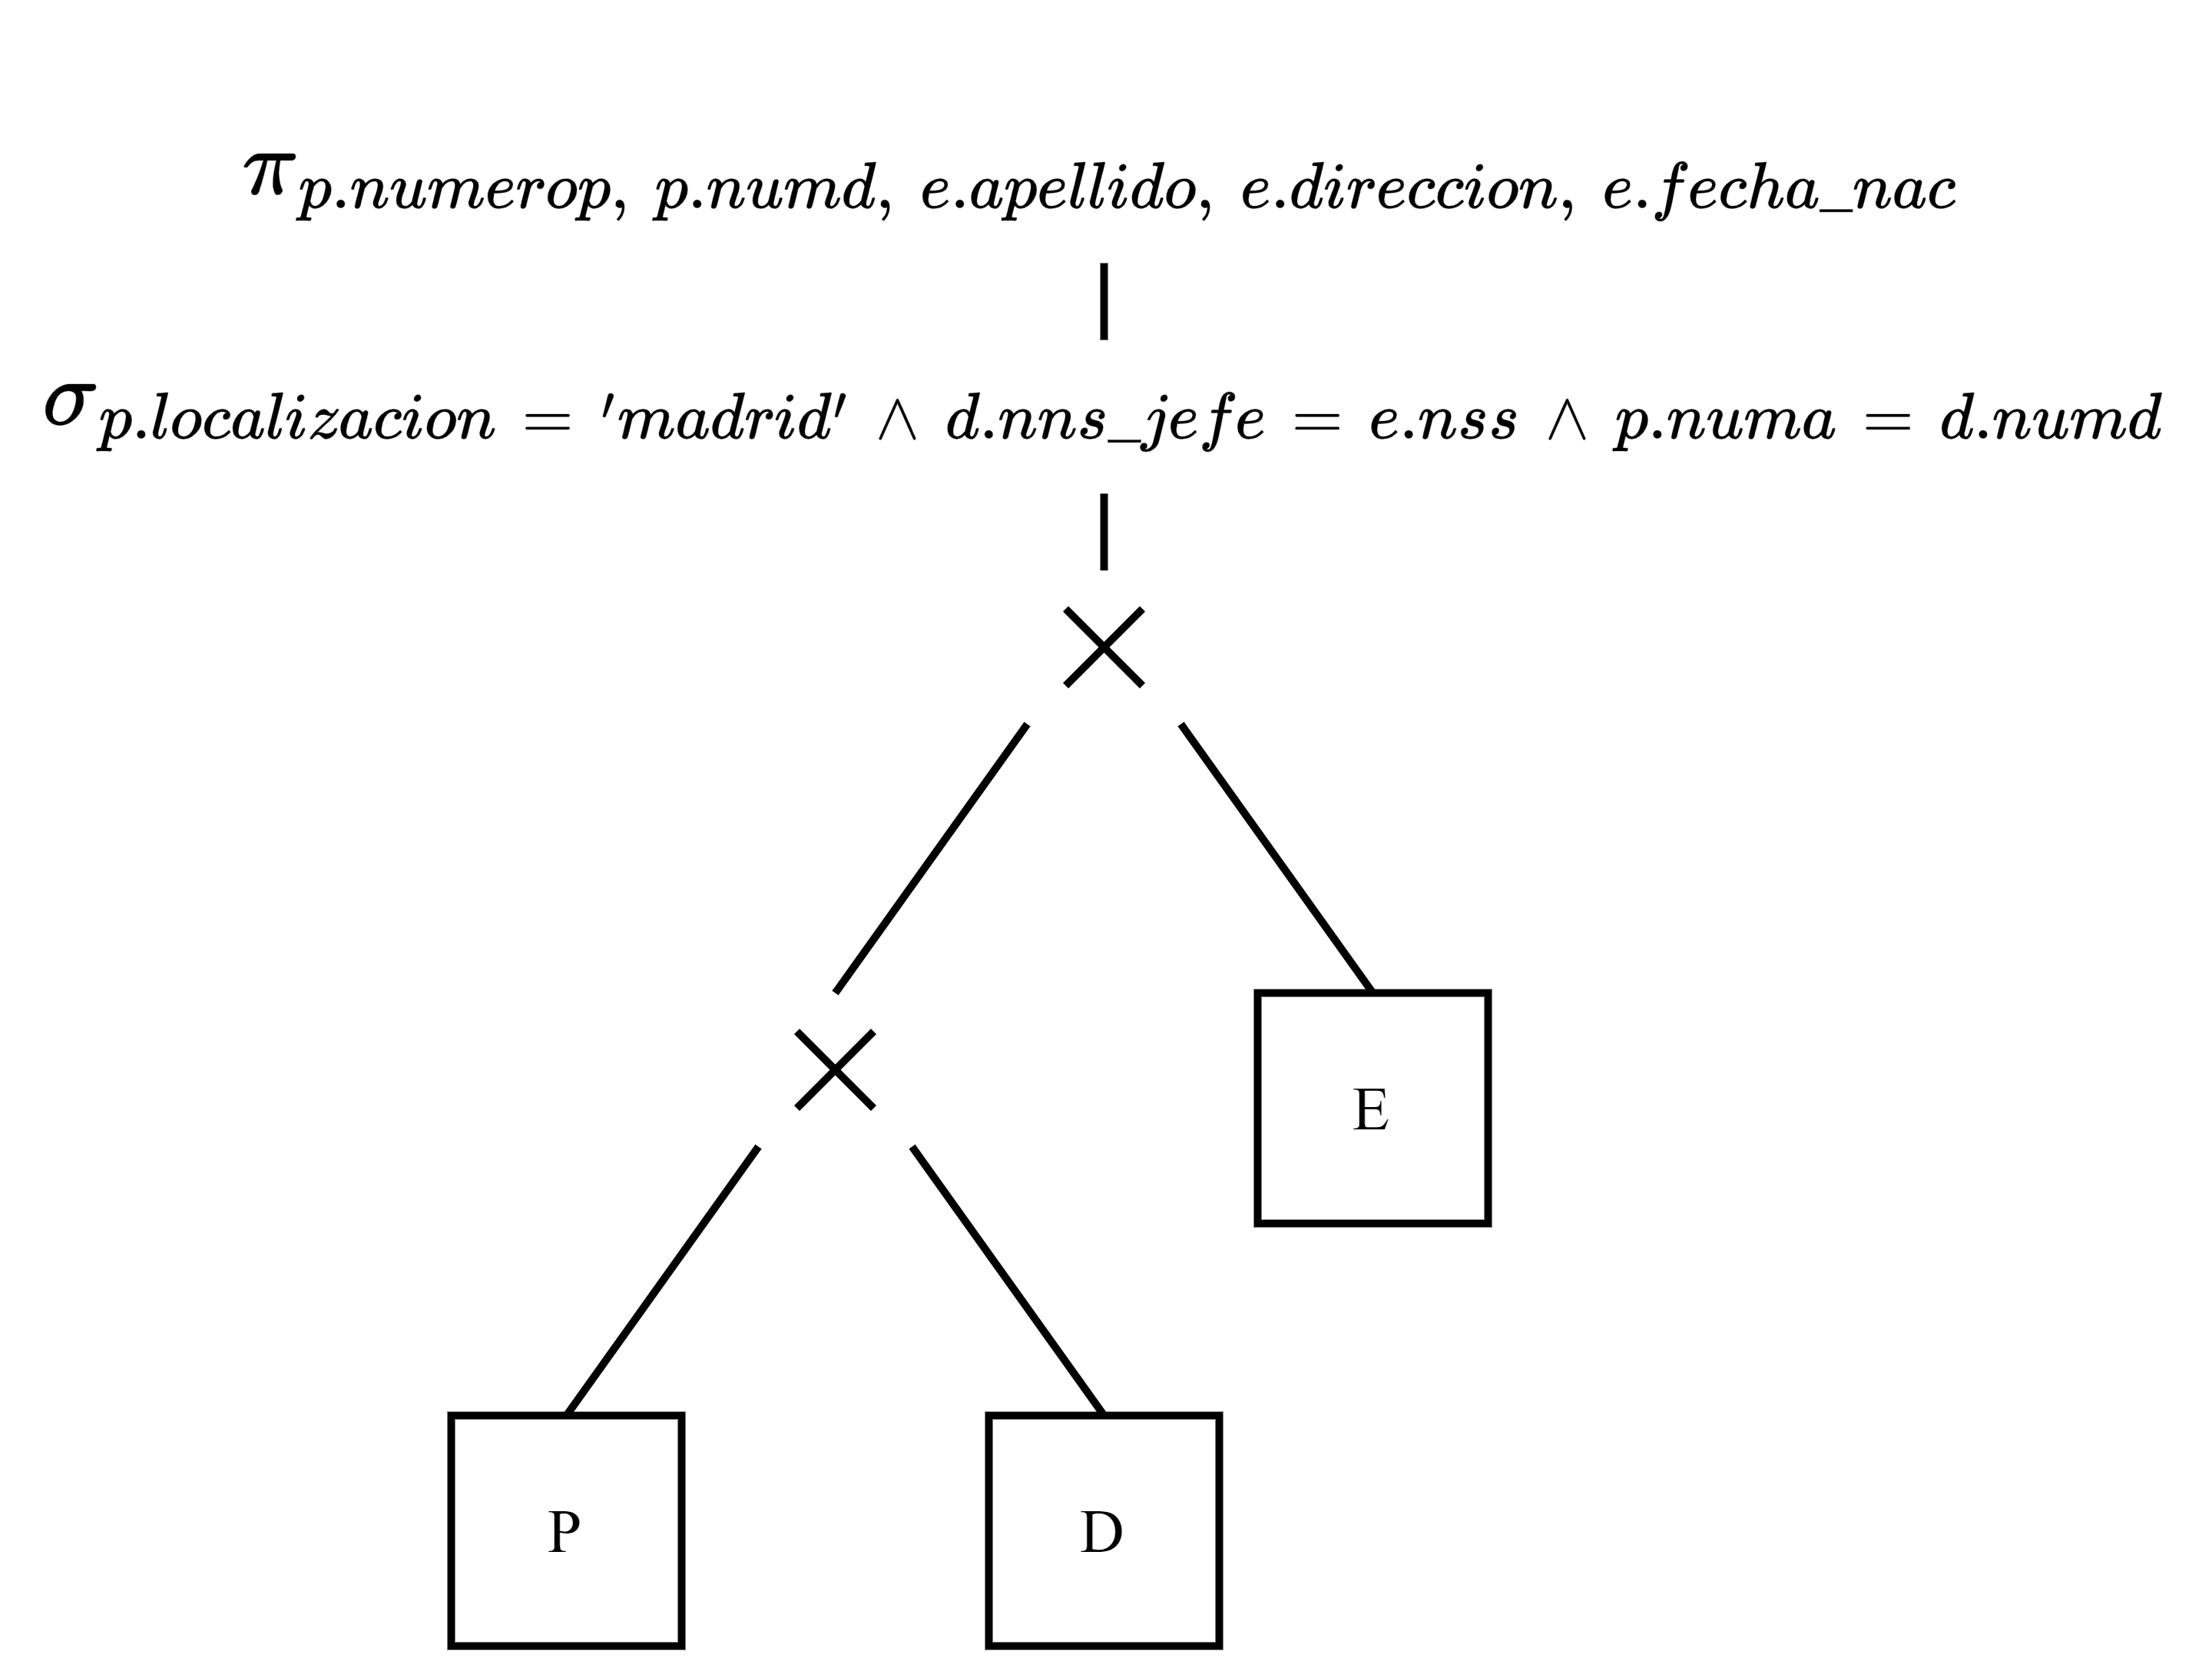
\includegraphics[width=0.8\textwidth]{img/E4-Canonico.png}
    \end{figure}

    \begin{itemize}
        \item Optimizar
        \begin{enumerate}
            \item Separar las selecciones.
            \begin{figure}[H]
                \centering
                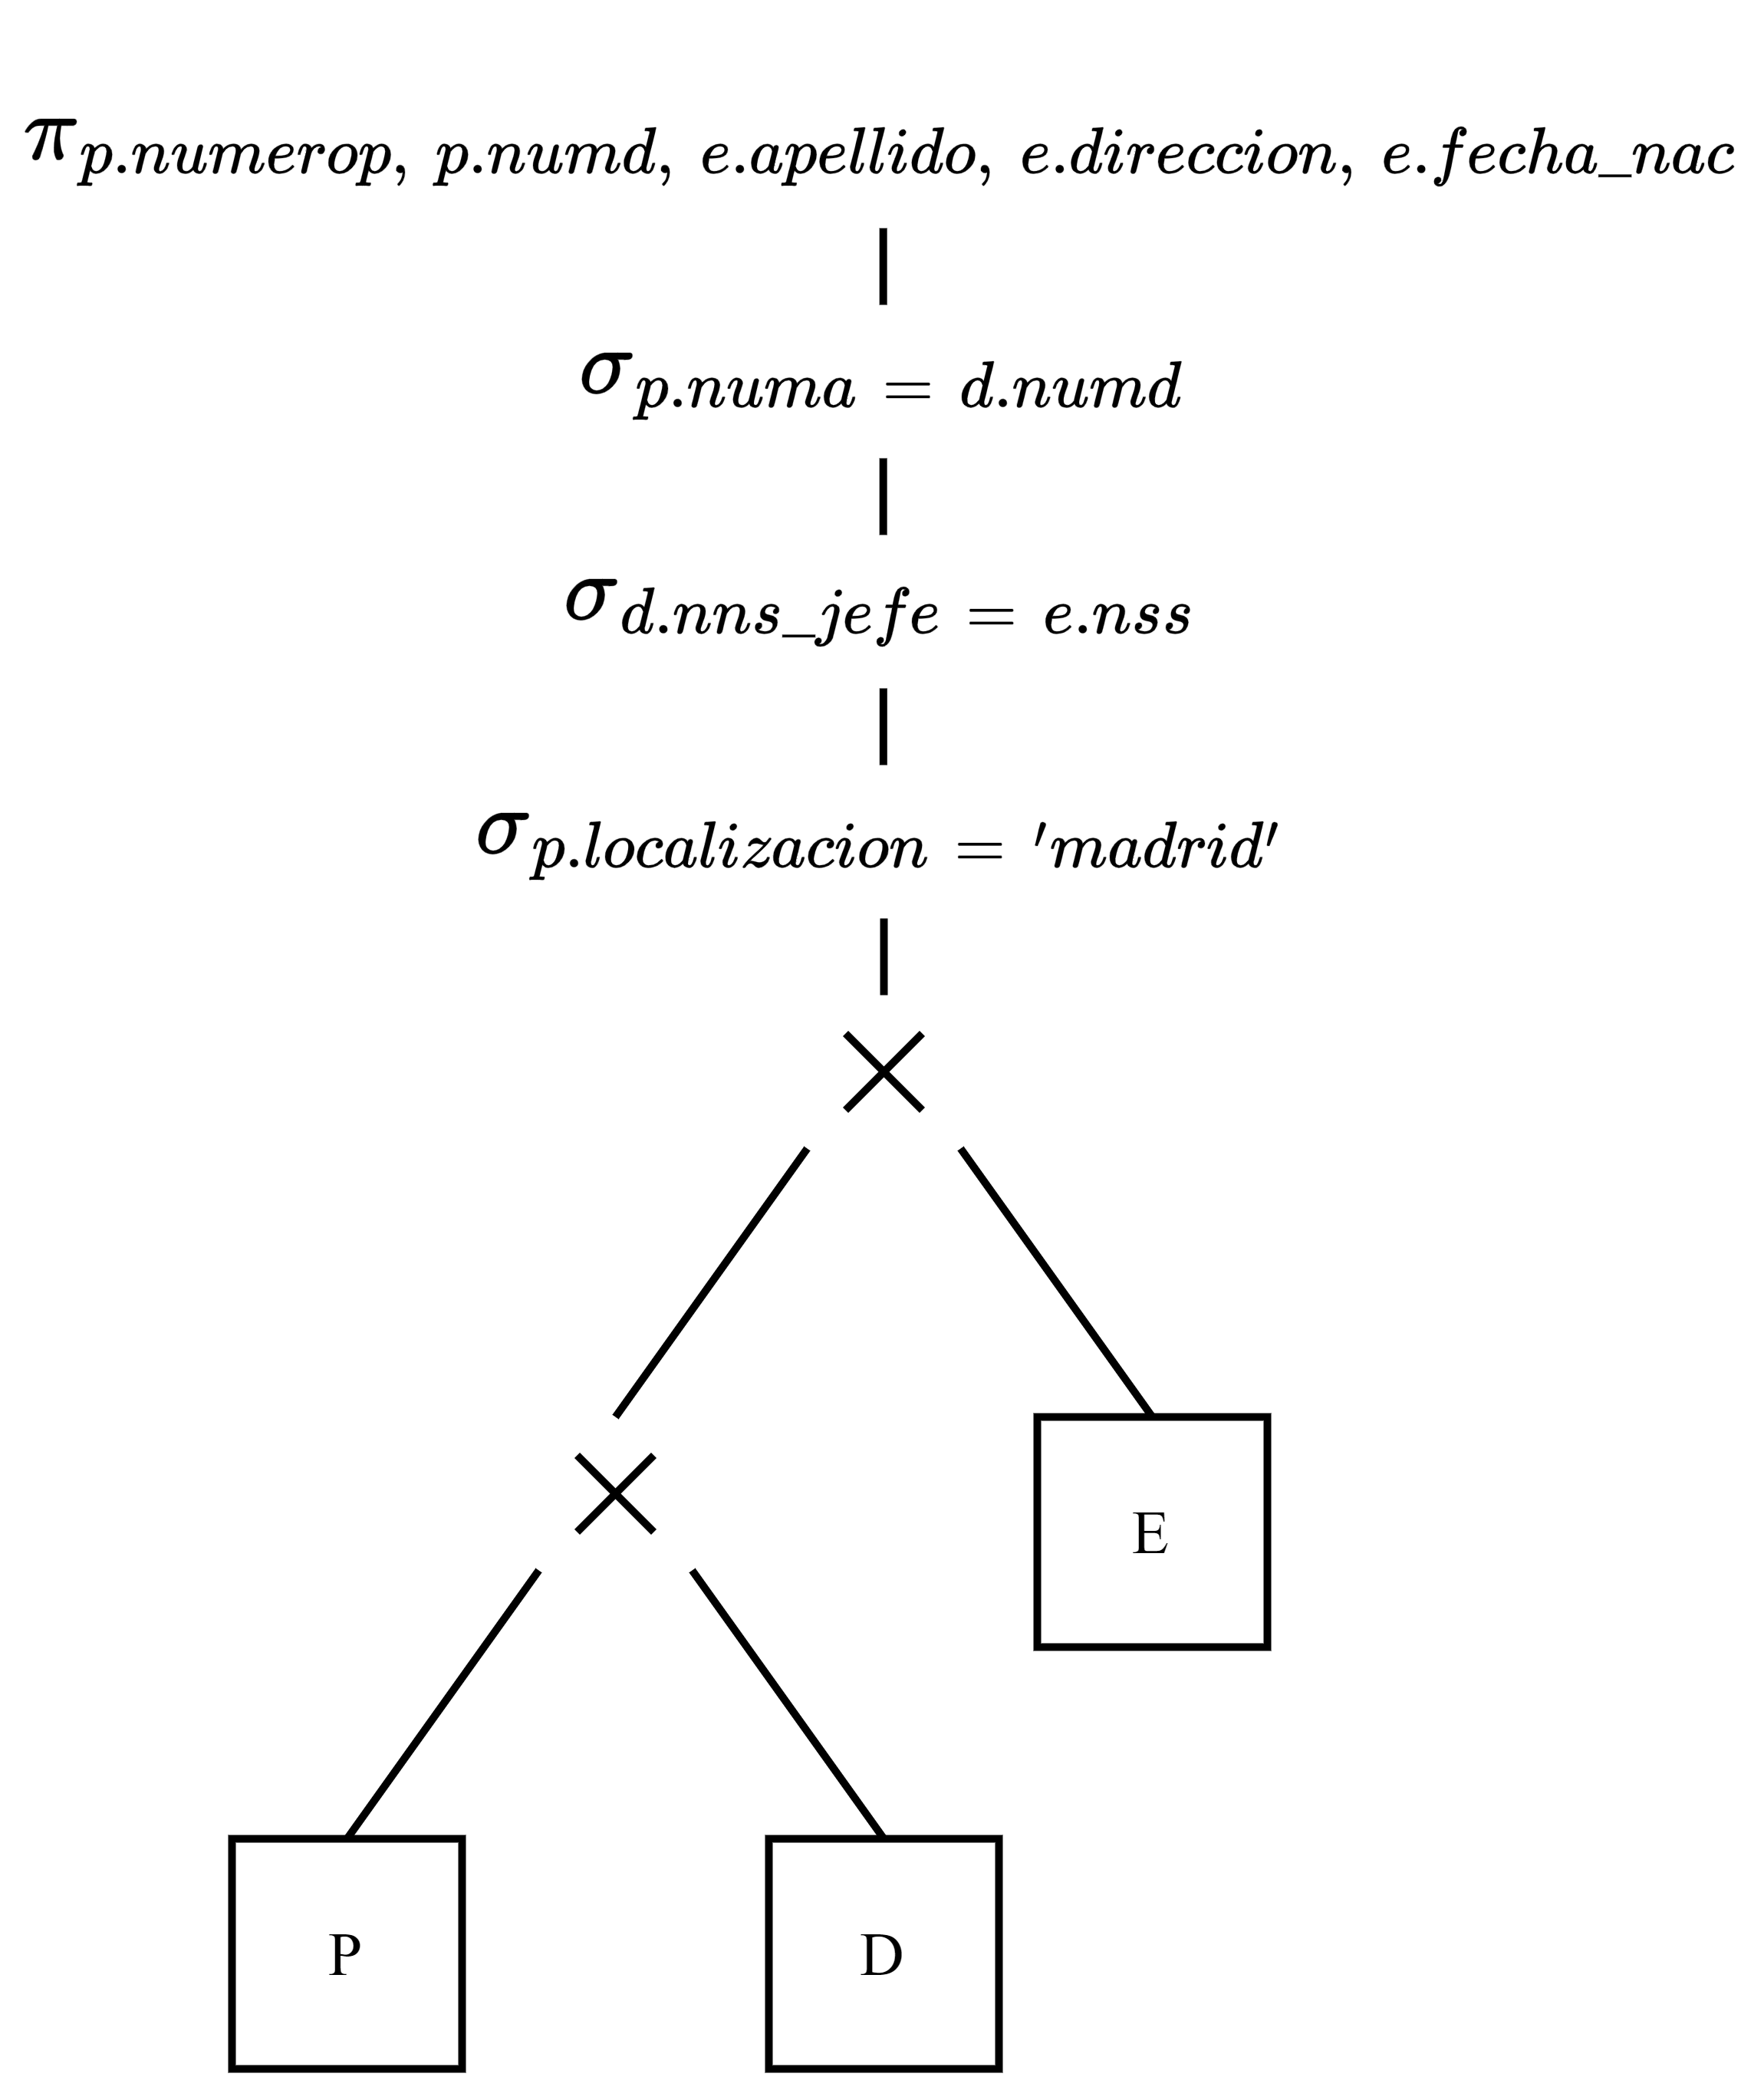
\includegraphics[width=0.6\textwidth]{img/E4-Paso-1.png}
            \end{figure}

            \newpage
            \item Permutar tablas si es necesario.

            \item Bajar las seleciones que son $\times$ para $\Join$.
            \begin{figure}[H]
                \centering
                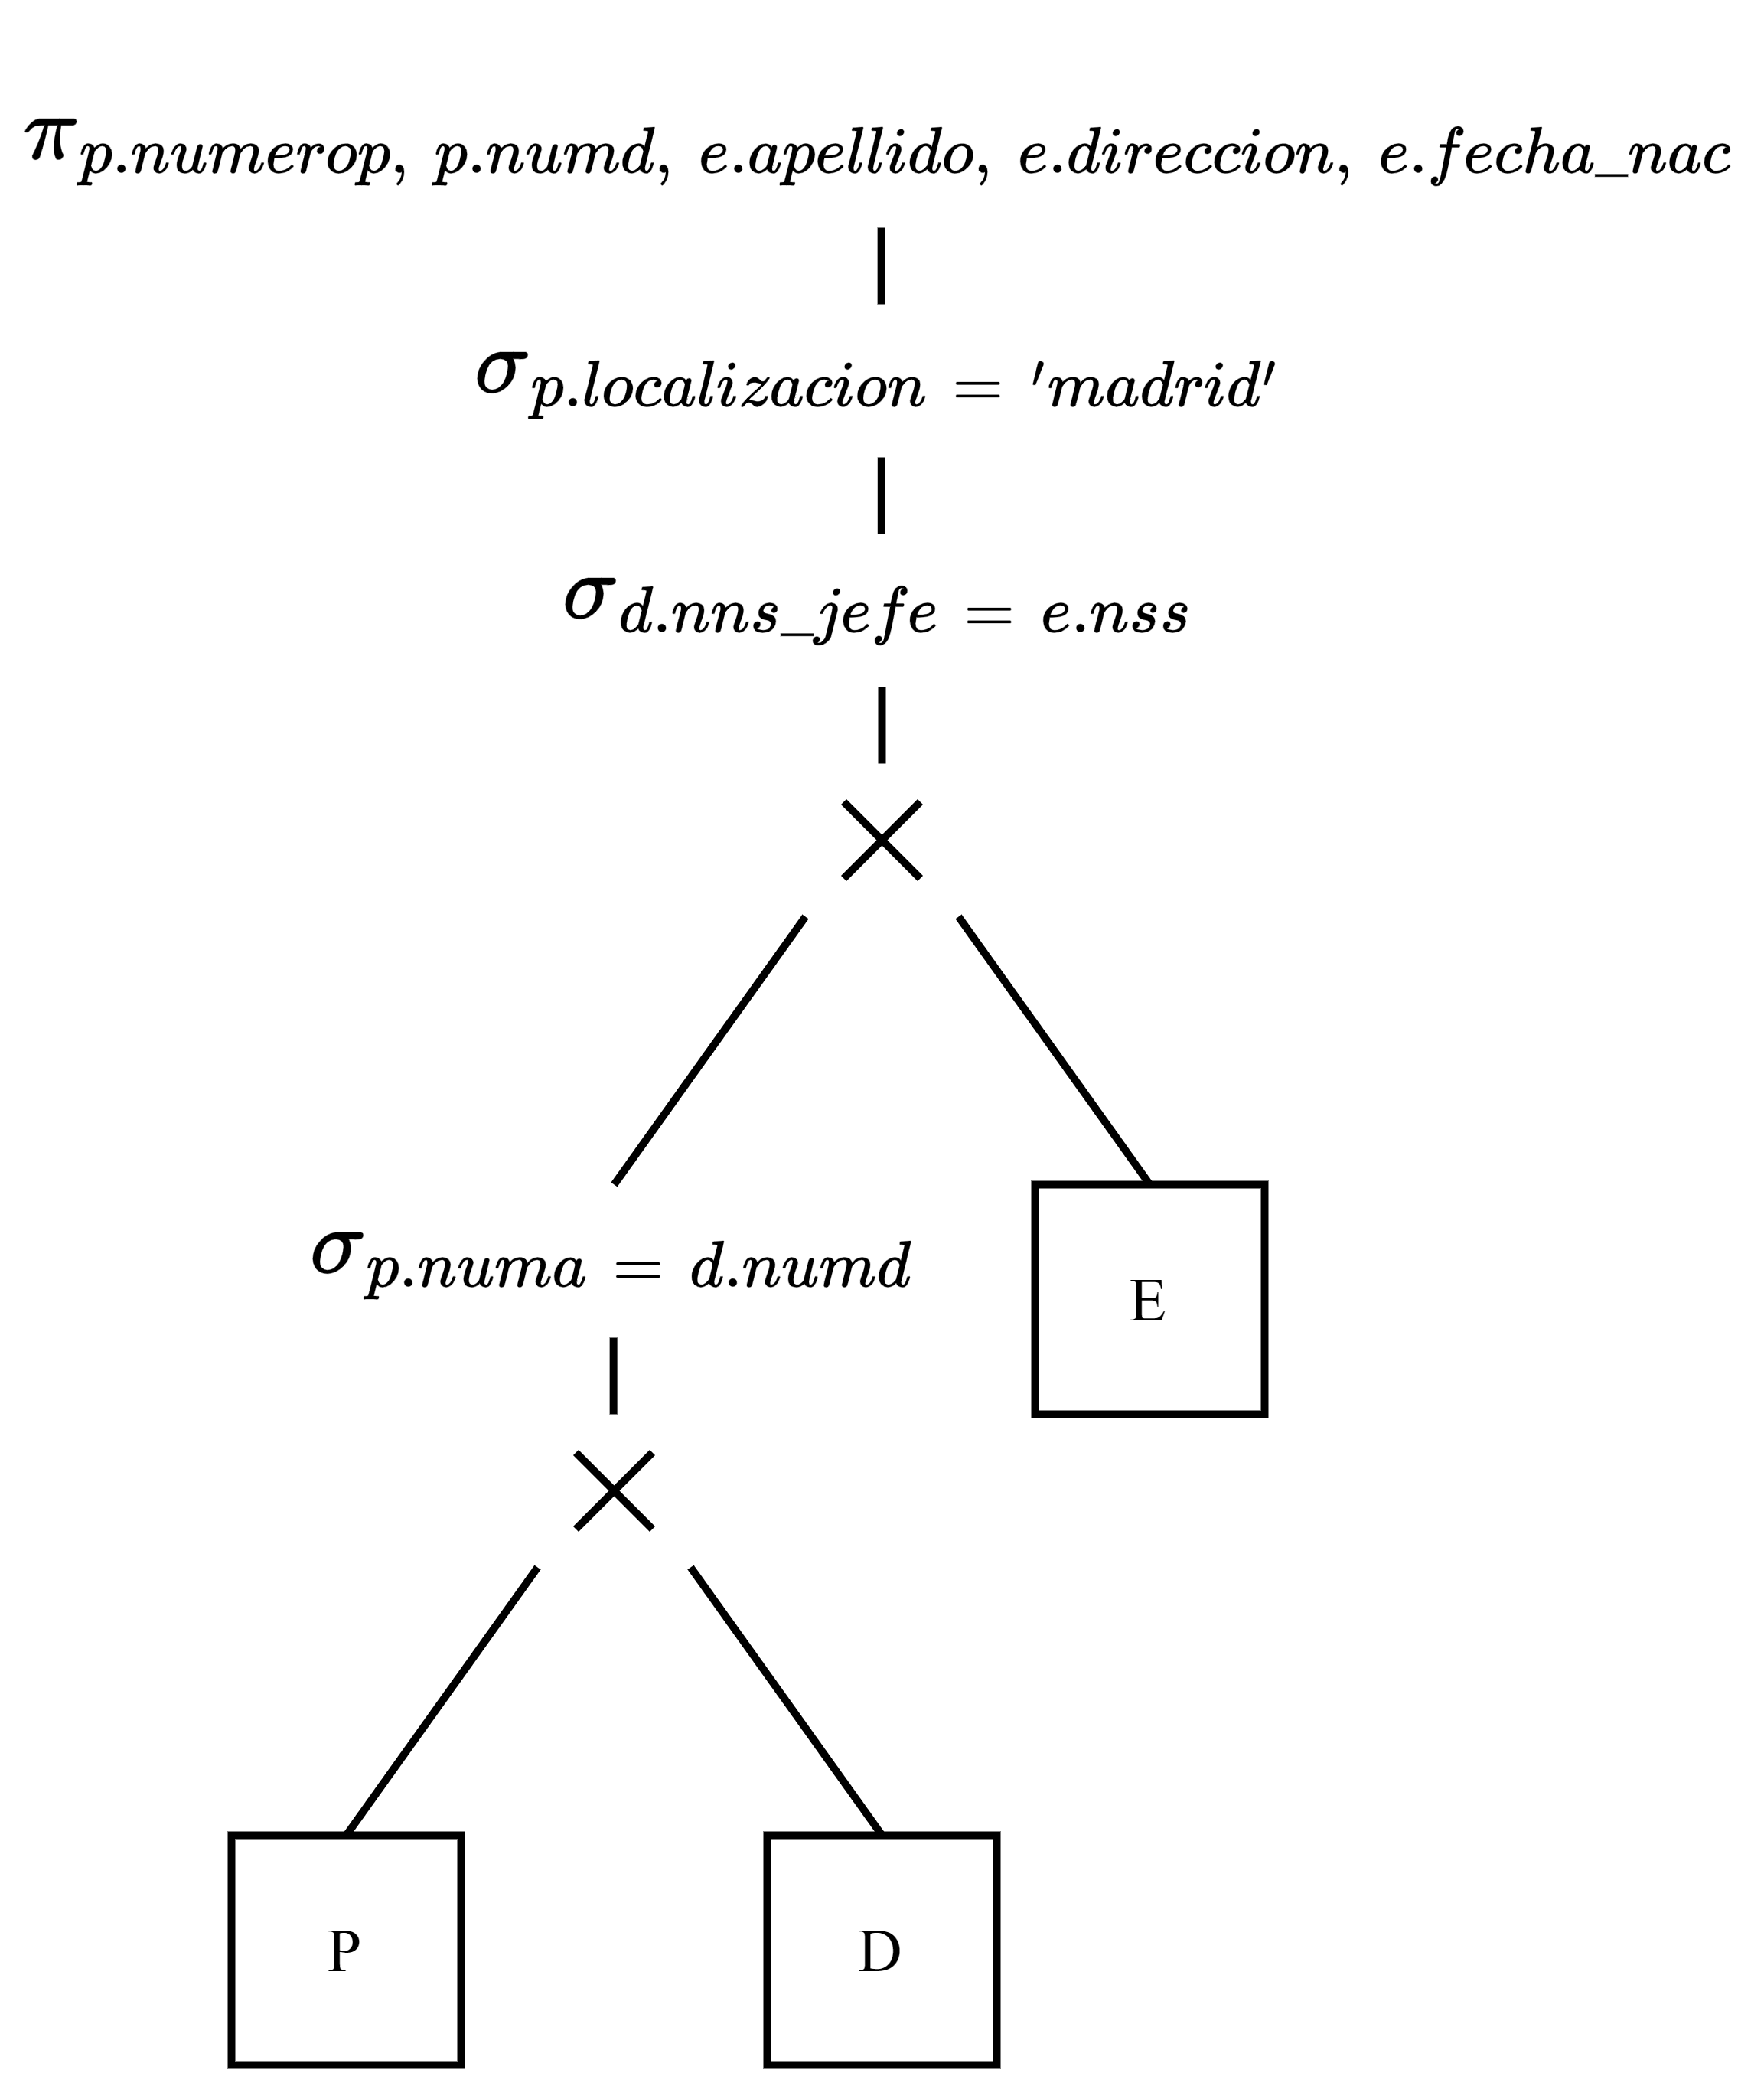
\includegraphics[width=0.6\textwidth]{img/E4-Paso-3.png}
            \end{figure}

            \item Cambio $\times$ por $\Join$.
            \begin{figure}[H]
                \centering
                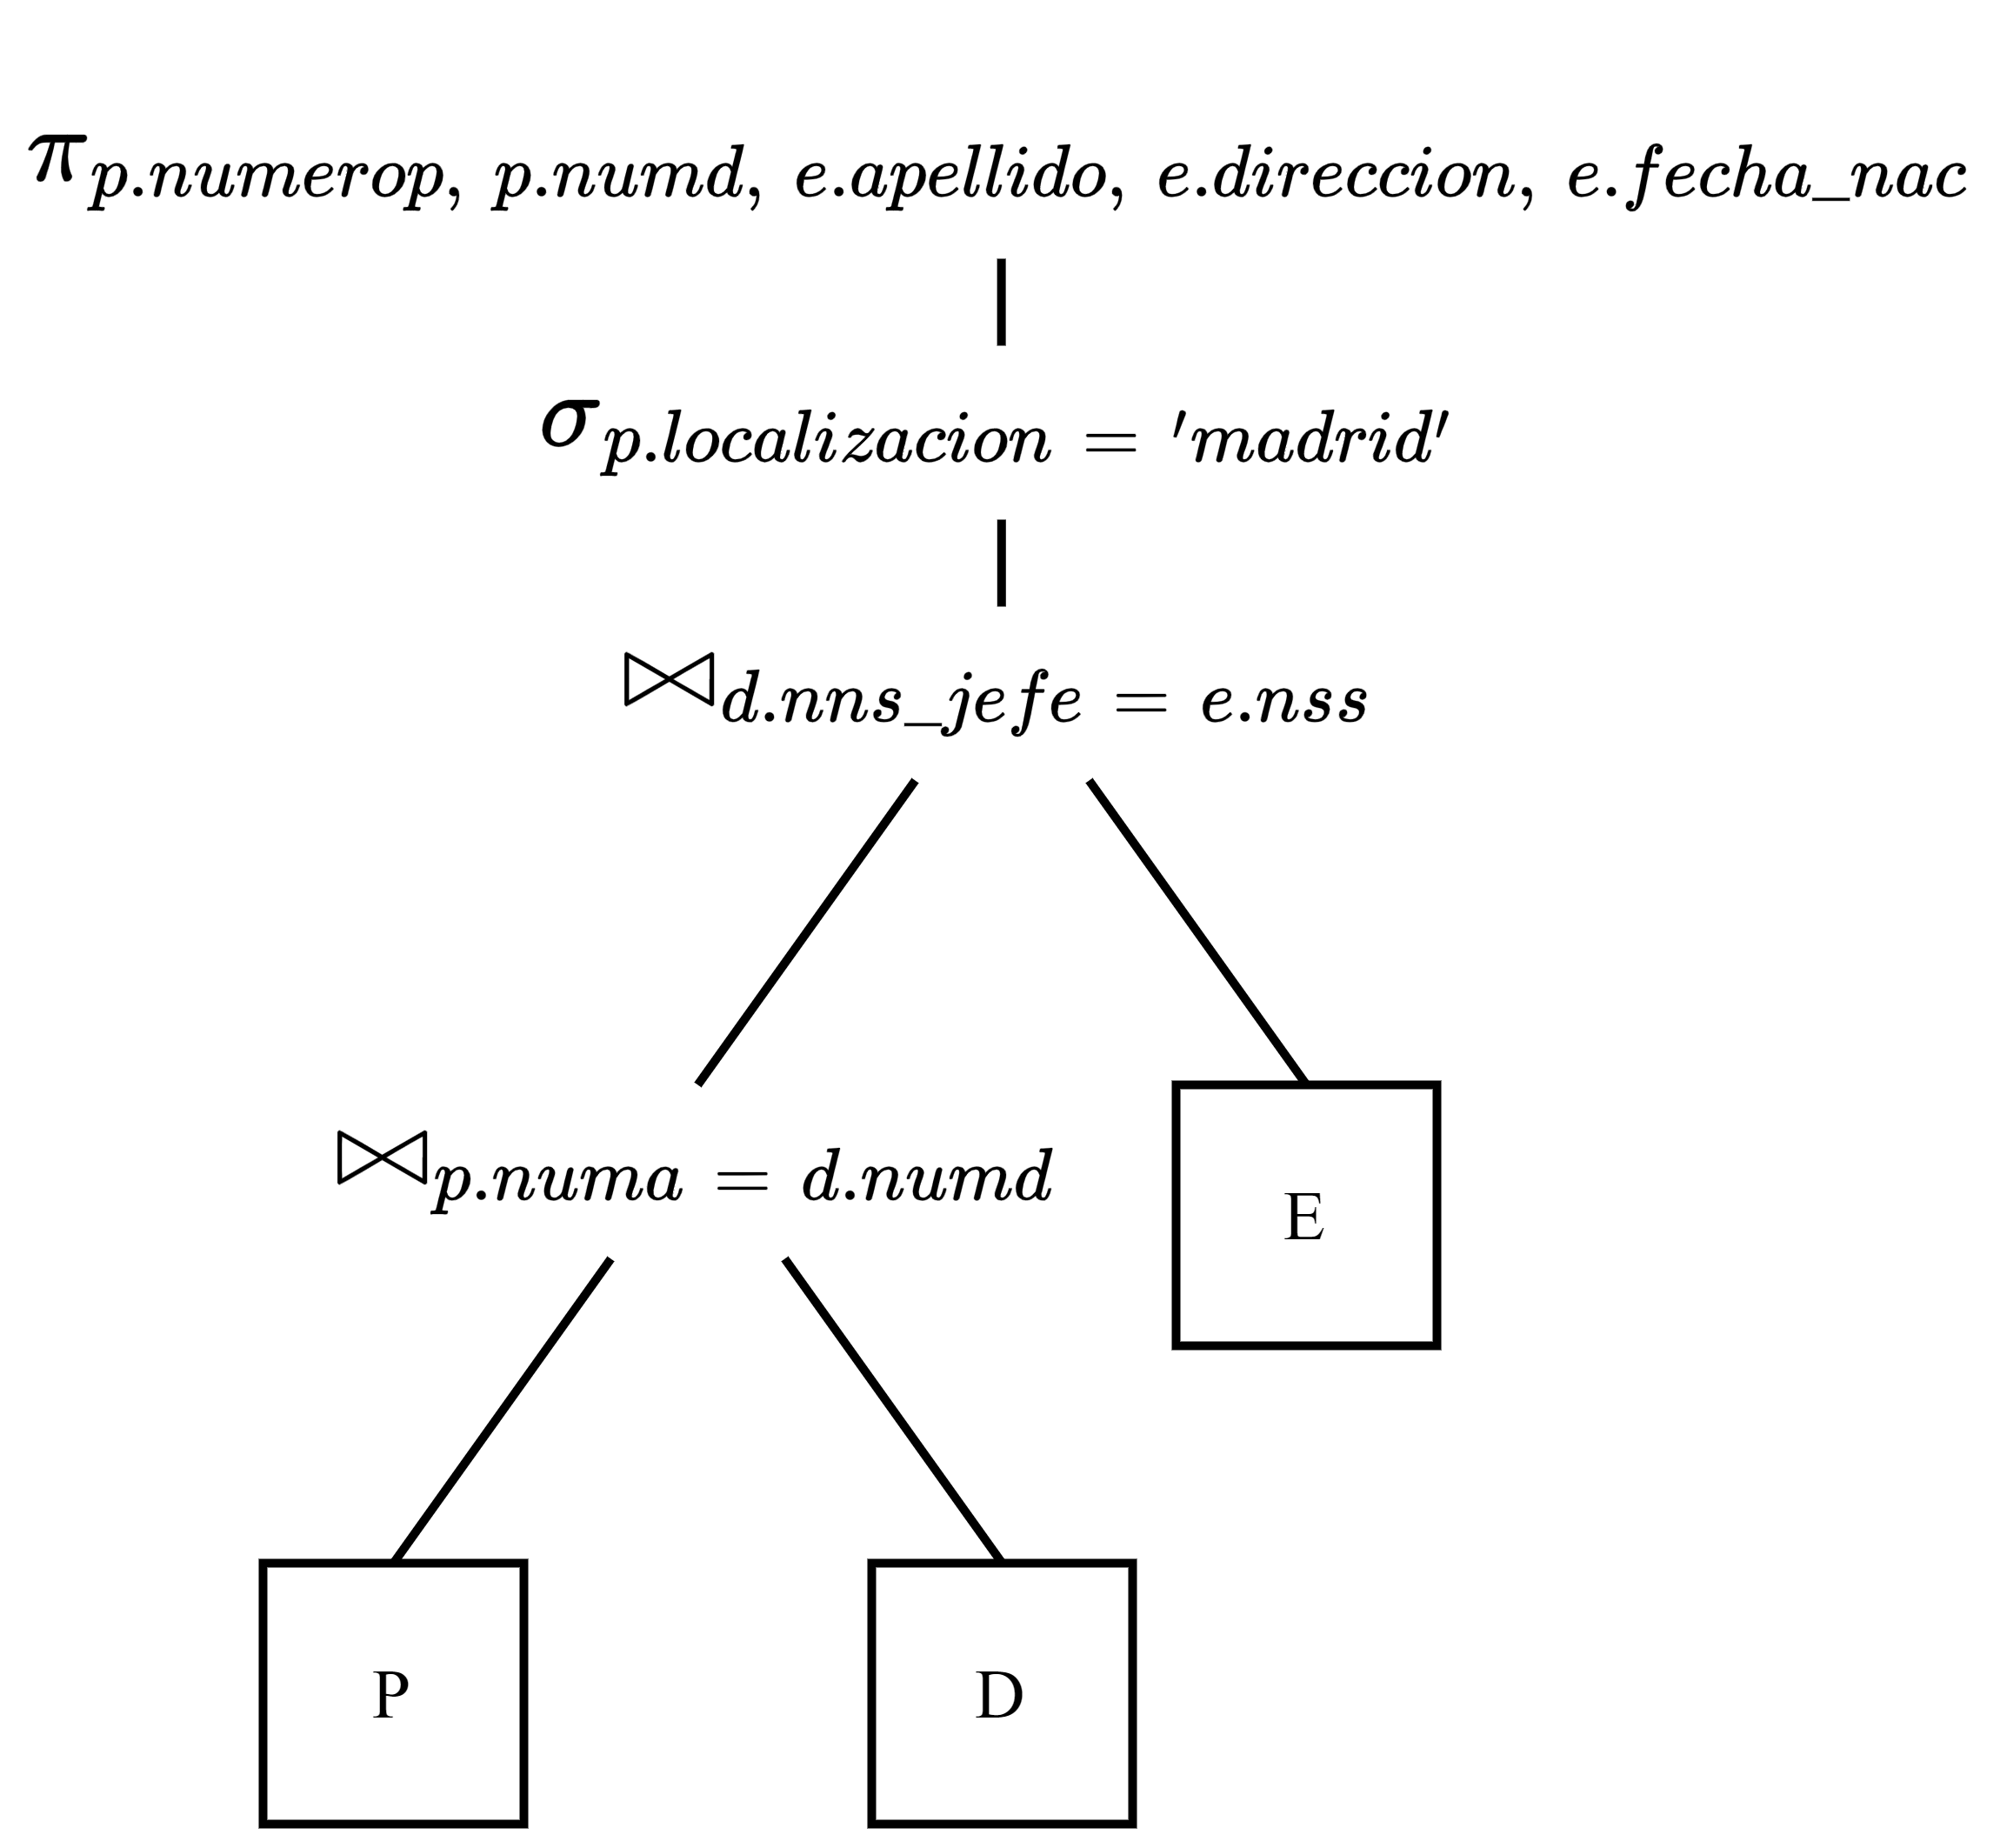
\includegraphics[width=0.6\textwidth]{img/E4-Paso-4.png}
            \end{figure}

            \newpage
            \item Bajar el resto de seleciones a tablas.
            \begin{figure}[H]
                \centering
                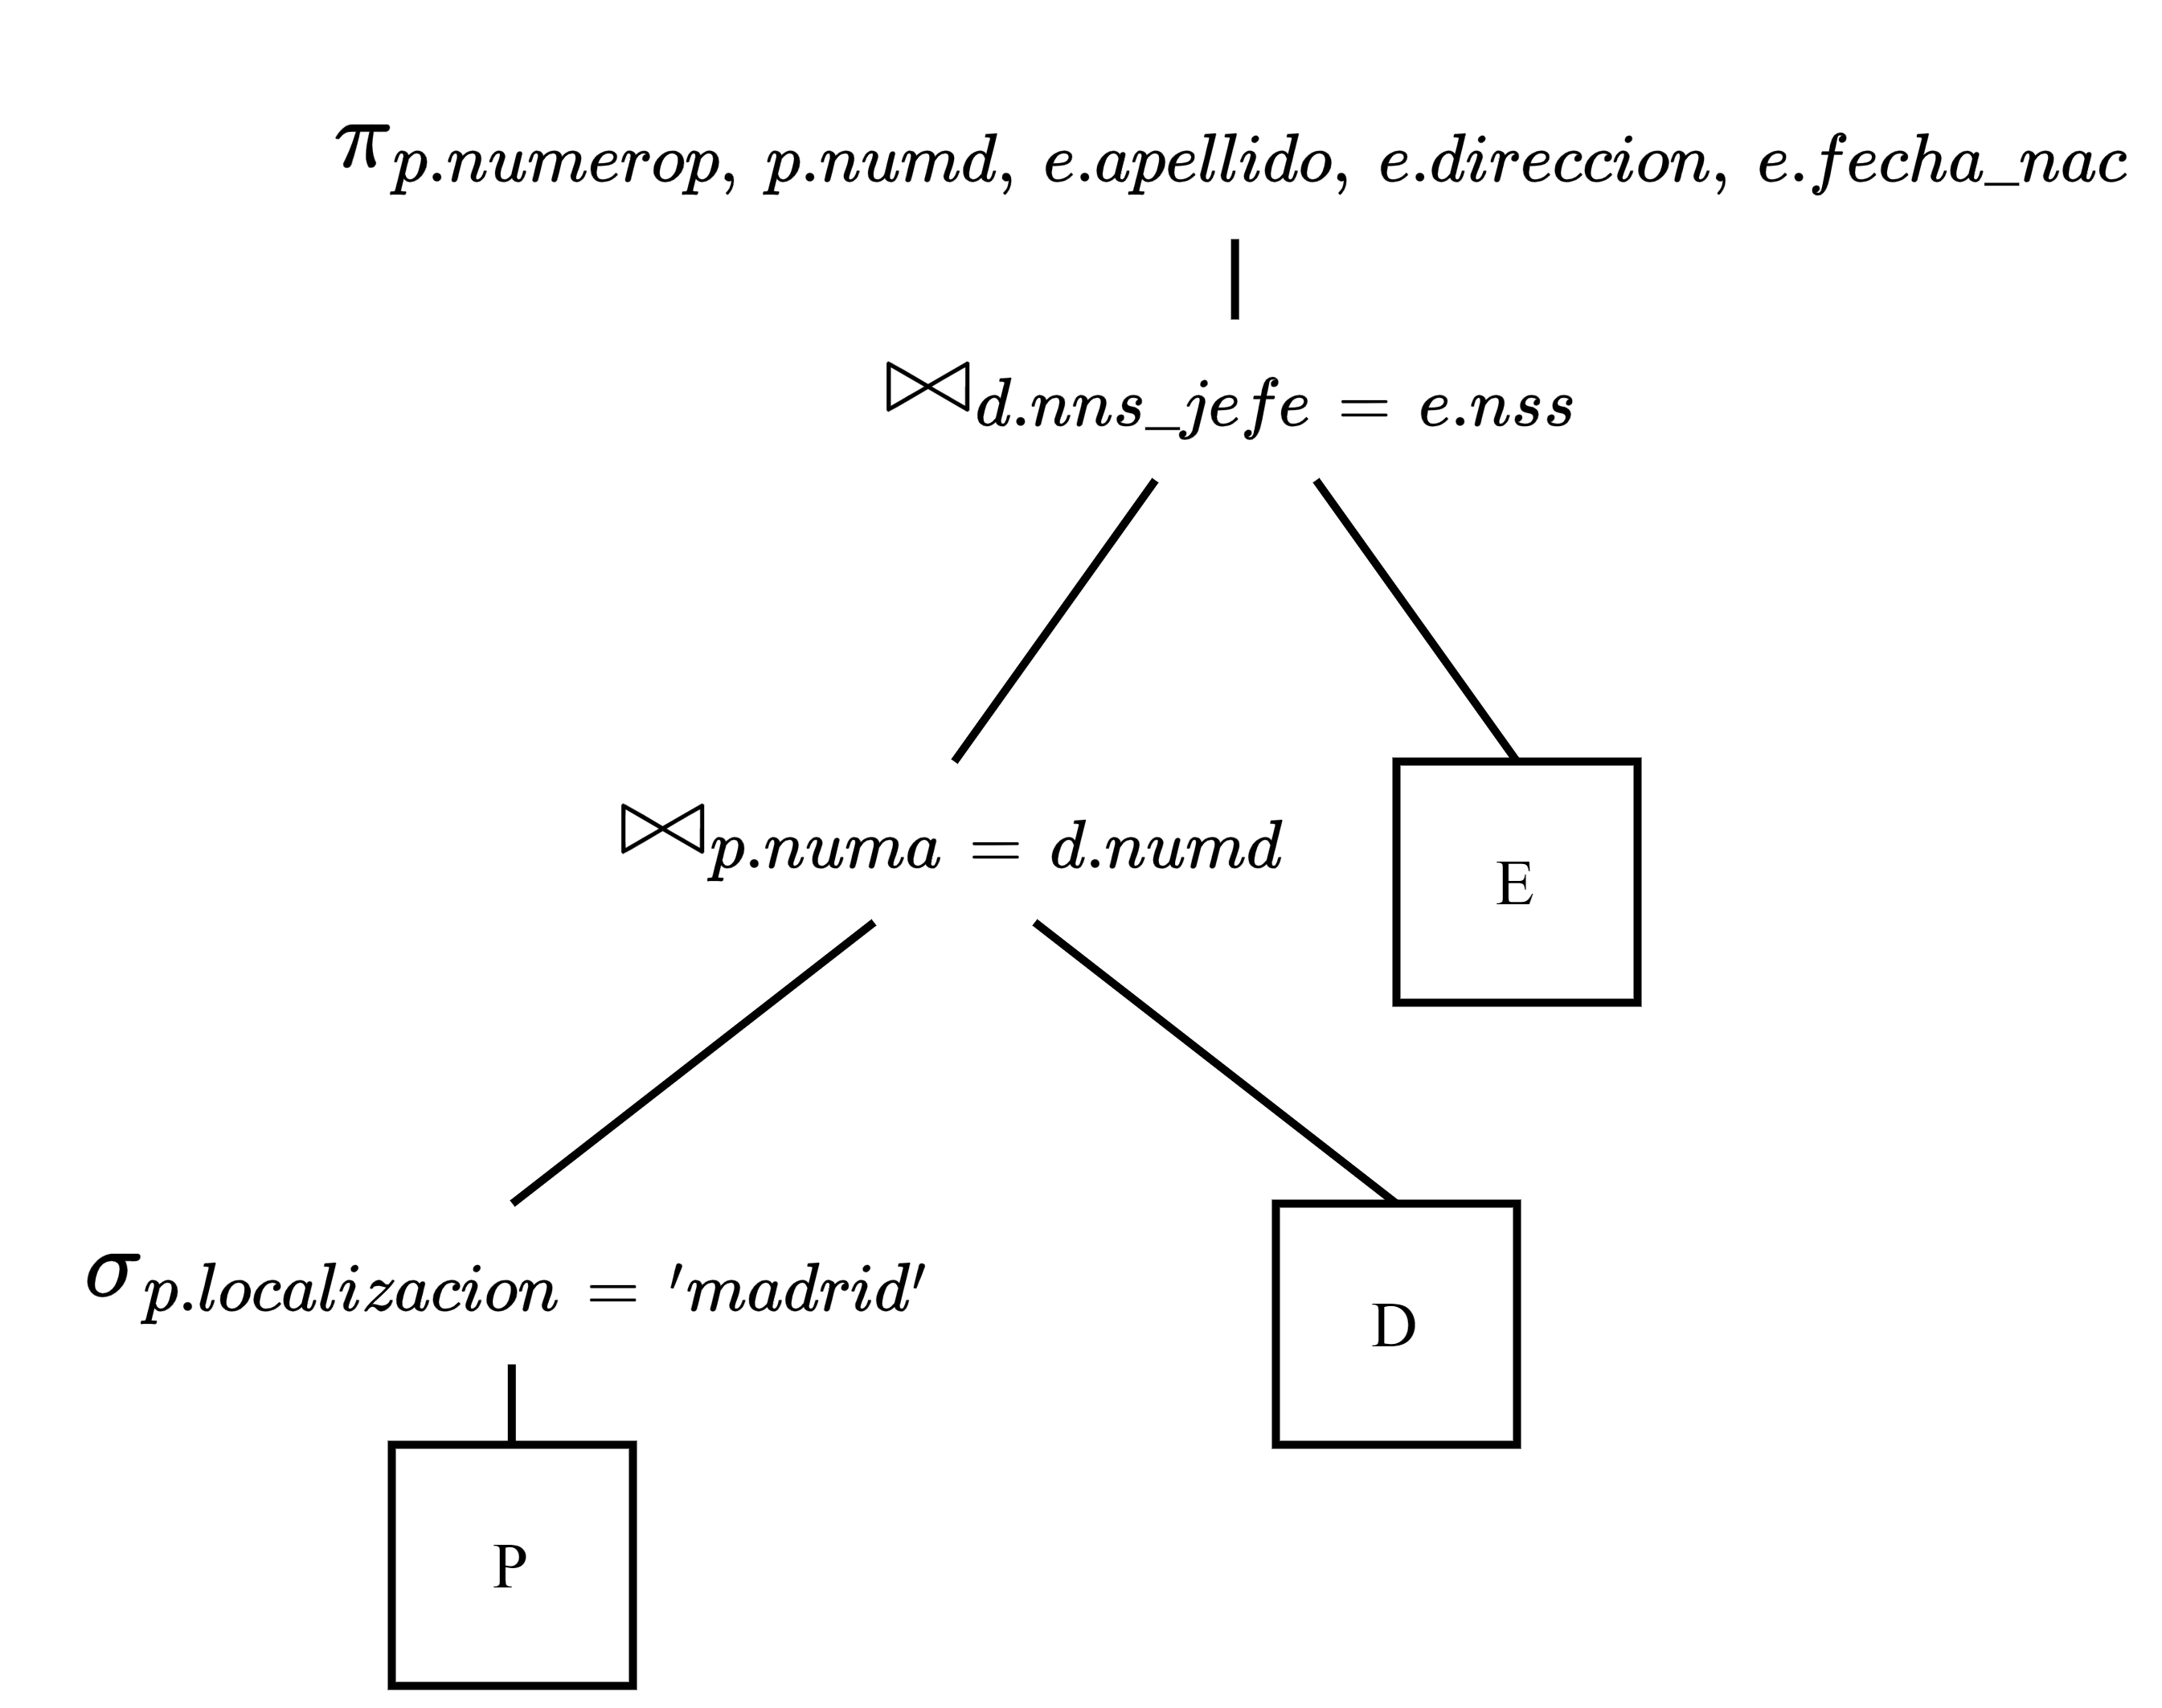
\includegraphics[width=0.7\textwidth]{img/E4-Paso-5.png}
            \end{figure}

            \item Proyectar los atributos necesarios.
            \begin{figure}[H]
                \centering
                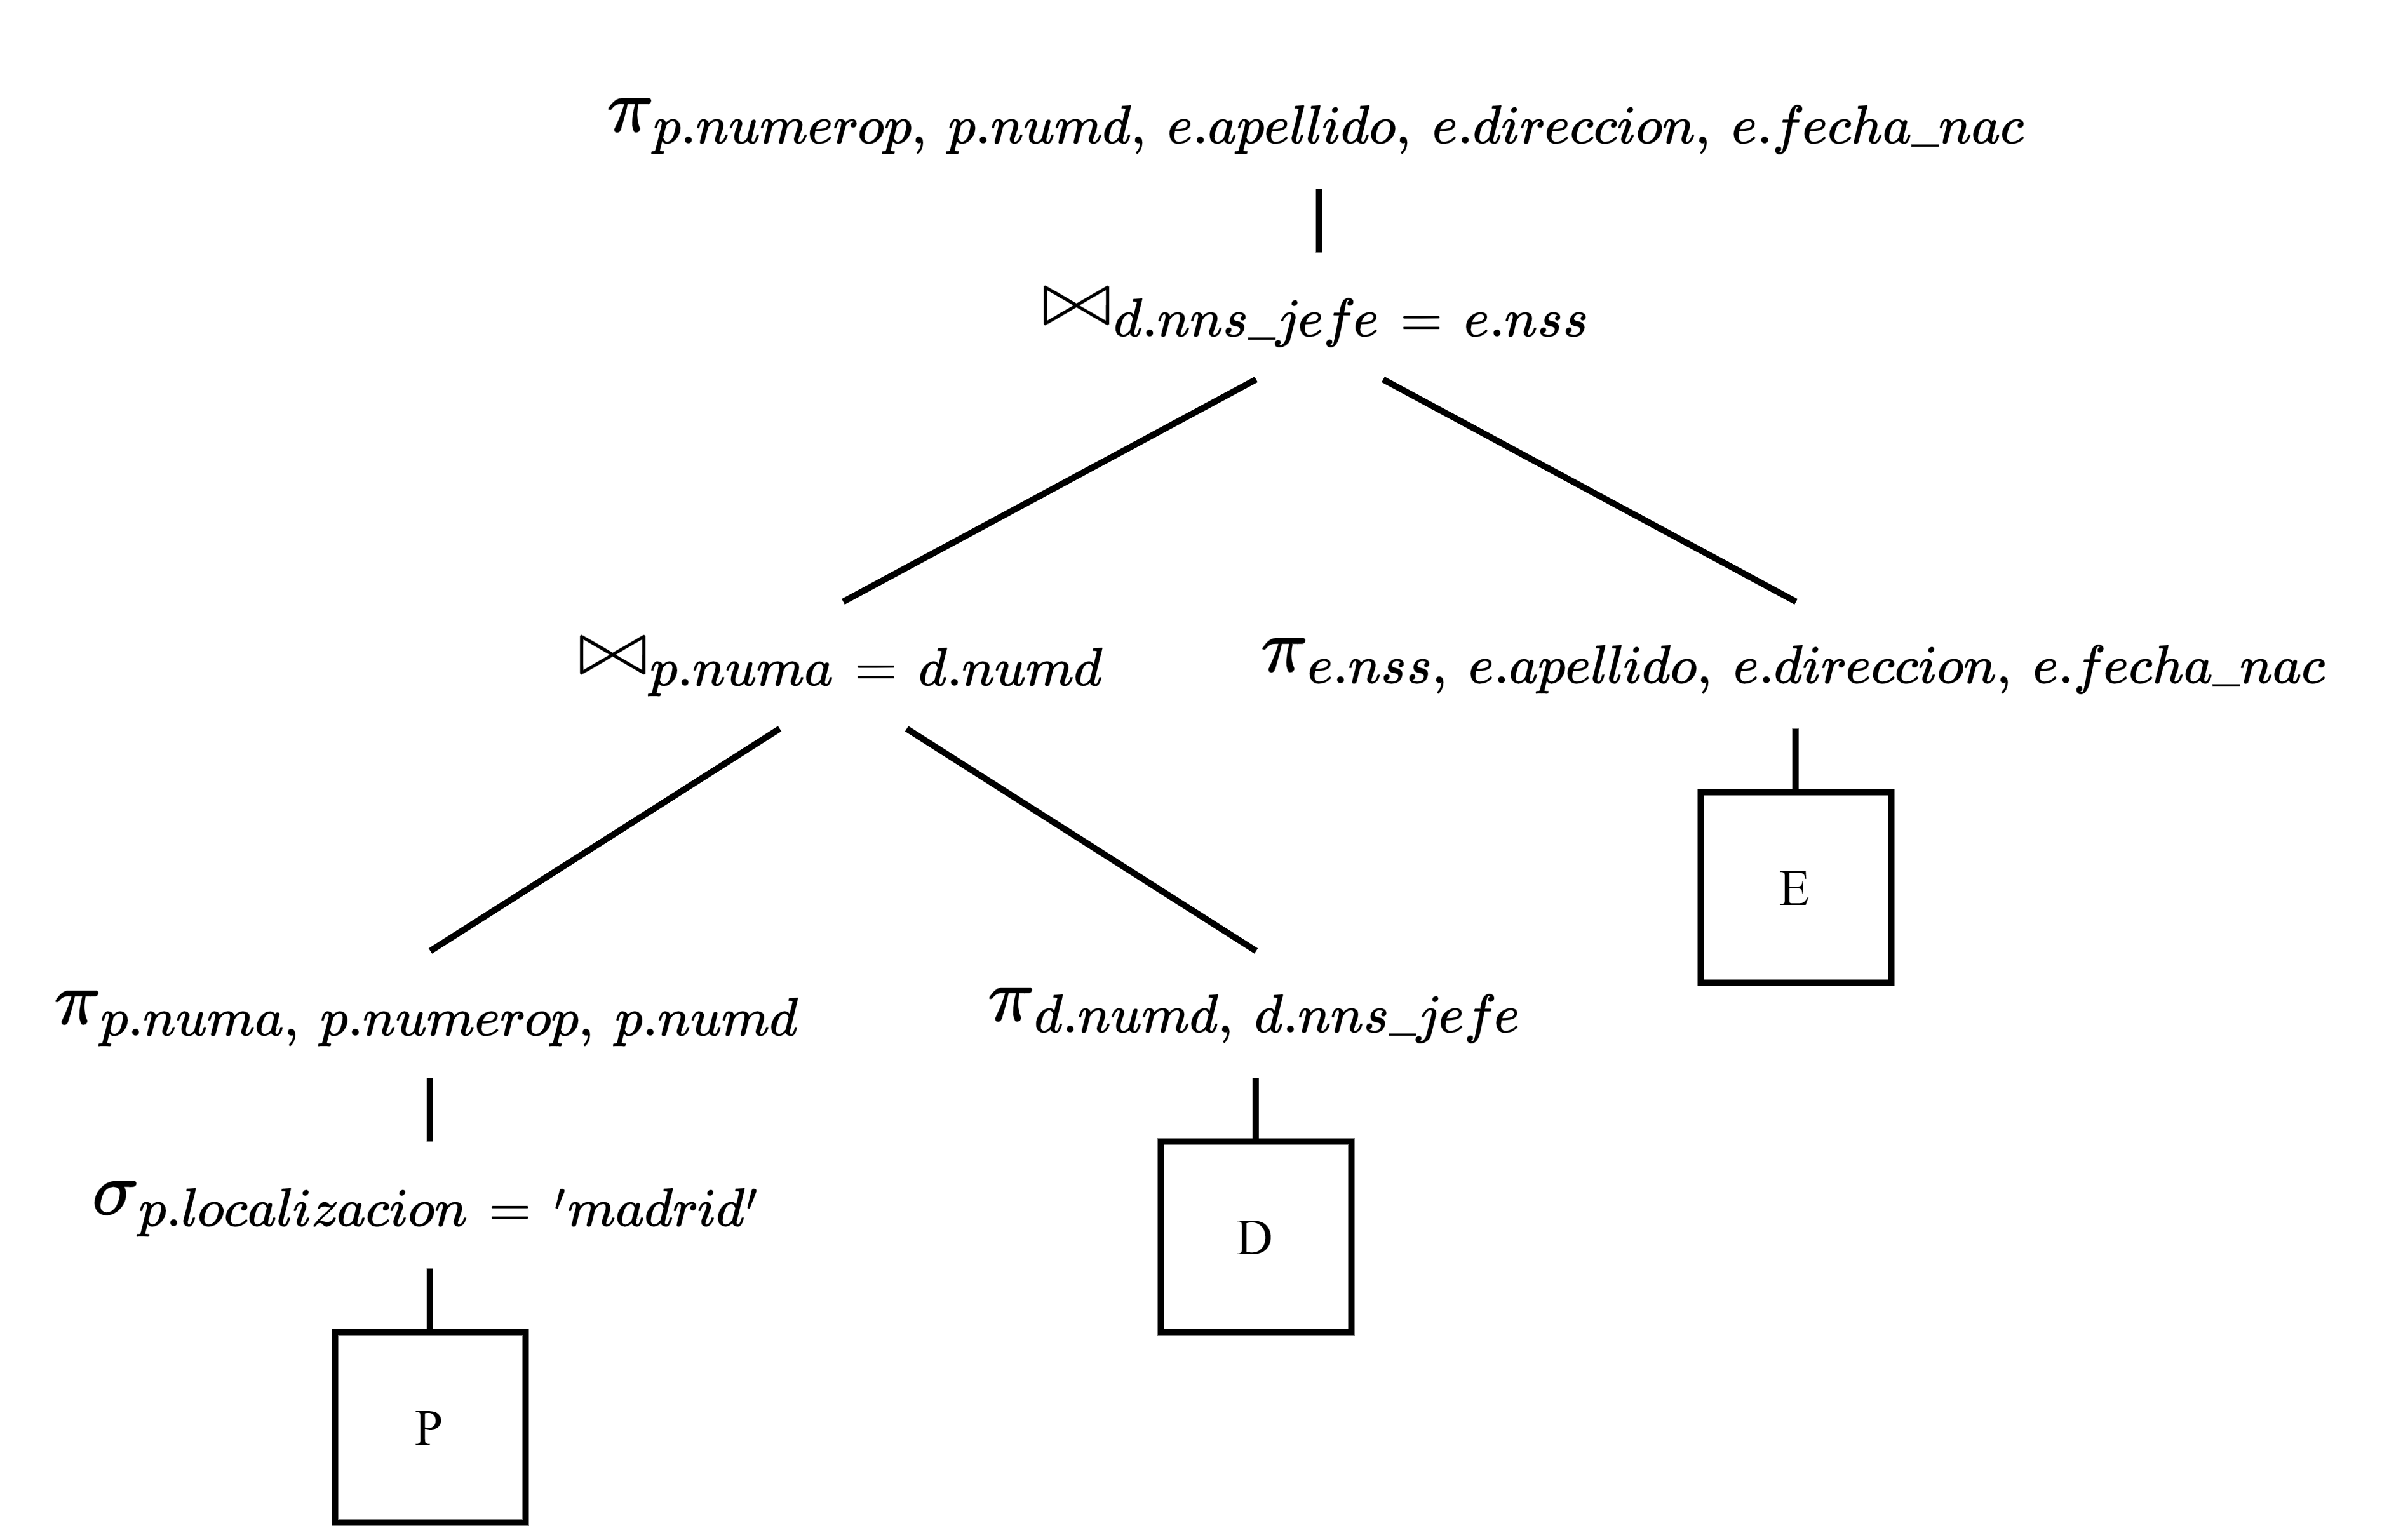
\includegraphics[width=\textwidth]{img/E4-Paso-6.png}
            \end{figure}
        \end{enumerate}
    \end{itemize}
\end{enumerate}
\end{document}